\documentclass[conference]{IEEEtran}
\IEEEoverridecommandlockouts
\usepackage{cite}
\usepackage{caption}
\captionsetup{justification=centering}

\usepackage{tabularx}
\usepackage{adjustbox}
\usepackage{booktabs}

\usepackage{amsmath,amssymb,amsfonts}
\usepackage{algorithmic}
\usepackage{graphicx}
\usepackage{textcomp}
\usepackage{longtable,float}
\usepackage[table]{xcolor}
\usepackage{subcaption}
\usepackage{blindtext}
\usepackage{setspace}
\usepackage{siunitx}
\usepackage{comment}
\usepackage{multirow}
\usepackage{threeparttable} 
\usepackage[font=small,skip=0pt]{caption}
\usepackage{blindtext}
\usepackage[a4paper, total={6in, 8in}]{geometry}


\usepackage[norule,hang]{footmisc}
\setlength{\footnotemargin}{1em}
\setlength{\skip\footins}{3em}

\usepackage{placeins}
\usepackage{afterpage}
\captionsetup[table]{skip=10pt}



\def\BibTeX{{\rm B\kern-.05em{\sc i\kern-.025em b}\kern-.08em
		T\kern-.1667em\lower.7ex\hbox{E}\kern-.125emX}}
\begin{document}	
	
	\onecolumn
	\title{Supplementary material to Robustness in Network Intrusion Detection with Adversarial Training and Ouf-of-Distribution
		%{\footnotesize \textsuperscript{*}Note: Sub-titles are not captured for https://ieeexplore.ieee.org  and
			%	should not be used}
		%\thanks{Identify applicable funding agency here. If none, %delete this.}
	}
	
	\author{Anonymous}
		
	
	
	\maketitle
	
	This document presents supplementary material that supports our main paper. It includes tables displaying the results obtained for the metrics discussed in the paper across the relevant datasets. The data presented here pertains to the ensemble trained on unperturbed samples (EnC) and the adversarial training (EnIDS). The graphs provided primarily correspond to the precision metric, with the exception of the "Out-of-Distribution" section. In this section, the ROC-AUC metric is used for the EnIDS model, which is abbreviated as IDS, and for out-of-distribution (OOD) detection.
	
	The sections in this supplement are organized according to adversarial attacks and out-of-distribution (OOD) scenarios, similar to the experiments section of the main paper. In the tables, blue-shaded cells indicate that the EnIDS model performed equally as well as the EnC model. In contrast, yellow-shaded cells signify that the EnIDS model outperformed the EnC model.	
	
	
	
	\section{Projected Gradient Descent (PGD-100)}
	
	\subsection{CIC IDS2017}
	
	\begin{table}[h]
		\caption{PGD-100 attack against EnC and EnIDS for binary classification on the CIC IDS2017 dataset.}
		\small
		\setlength{\tabcolsep}{1.6pt}
		\centering
		\label{tab:cic_bin_pgd}
		\begin{tabular}{|c|c|c|c|c|c|c|c|c|c|c|c|c|}
			\hline
			\multirow{3}{*}{\textbf{Type}} & \multirow{3}{*}{\textbf{Norm}} & \multirow{3}{*}{\textbf{Metric}} & \multicolumn{10}{c|}{\textbf{\textsl{Epsilon} ($\epsilon$)}} \\
			\cline{4-13}
			& & & \multicolumn{2}{c|}{\textbf{0.008}} & \multicolumn{2}{c|}{\textbf{0.01}} & \multicolumn{2}{c|}{\textbf{0.03}} & \multicolumn{2}{c|}{\textbf{0.05}} & \multicolumn{2}{c|}{\textbf{0.08}} \\
			\cline{4-13}
			& & & \textbf{\textsl{Benign}} & \textbf{\textsl{Attacks}} & \textbf{\textsl{Benign}} & \textbf{\textsl{Attacks}} & \textbf{\textsl{Benign}} & \textbf{\textsl{Attacks}} & \textbf{\textsl{Benign}} & \textbf{\textsl{Attacks}} & \textbf{\textsl{Benign}} & \textbf{\textsl{Attacks}} \\
			\hline
			\multirow{9}{*}{EnC} 
			& \multirow{3}{*}{\( \ell_1 \)} & Precision & 99.99 & 98.85 & 99.99 & 98.84 & 99.99 & 98.78 & 99.99 & 98.73 & 99.99 & 98.67 \\
			& & Recall & 99.76 & 99.95 & 99.76 & 99.94 & 99.75 & 99.94 & 99.74 & 99.94 & 99.73 & 99.94 \\
			& & ROC-AUC & 100.00 & 100.00 & 100.00 & 100.00 & 100.00 & 100.00 & 99.99 & 100.00 & 99.99 & 100.00 \\
			\cline{2-13}
			& \multirow{3}{*}{\( \ell_2 \)} & Precision & 99.99 & 98.77 & 99.99 & 98.74 & 99.99 & 98.51 & 99.97 & 98.05 & 99.83 & 96.23 \\
			& & Recall & 99.75 & 99.94 & 99.74 & 99.94 & 99.69 & 99.93 & 99.59 & 99.83 & 99.21 & 99.16 \\
			& & ROC-AUC & 100.00 & 100.00 & 99.99 & 100.00 & 99.99 & 99.99 & 99.99 & 99.99 & 99.95 & 99.95 \\
			\cline{2-13}
			& \multirow{3}{*}{\( \ell_\infty \)} & Precision & 99.98 & 98.34 & 99.98 & 98.12 & 99.37 & 86.50 & 92.39 & 48.56 & 77.24 & 1.22 \\
			& & Recall & 99.66 & 99.92 & 99.61 & 99.89 & 96.92 & 96.97 & 85.90 & 65.28 & 67.83 & 1.95 \\
			& & ROC-AUC & 99.99 & 99.99 & 99.99 & 99.99 & 99.44 & 99.47 & 87.17 & 87.17 & 22.53 & 22.45 \\
			\hline
			\multirow{9}{*}{EnIDS} 
			& \multirow{3}{*}{\( \ell_1 \)} & Precision & 99.98 & 99.11 & 99.98 & 99.10 & 99.96 & \cellcolor{yellow!50}98.83 & 99.83 & \cellcolor{yellow!50}98.79 & 99.83 & \cellcolor{yellow!50}98.72 \\
			& & Recall & \cellcolor{yellow!50}99.82 & 99.89 & \cellcolor{yellow!50}99.82 & 99.89 & \cellcolor{yellow!50}99.76 & 99.82 & \cellcolor{yellow!50}99.75 & 99.17 & \cellcolor{yellow!50}99.74 & 99.16 \\
			& & ROC-AUC & 99.98 & 99.99 & 99.98 & 99.99 & 99.98 & 99.99 & 99.98 & 99.99 & 99.98 & 99.98 \\
			\cline{2-13}
			& \multirow{3}{*}{\( \ell_2 \)} & Precision & 99.98 & \cellcolor{yellow!50}99.04 & 99.97 & \cellcolor{yellow!50}99.01 & 99.83 & \cellcolor{yellow!50}98.77 & 99.82 & \cellcolor{yellow!50}98.62 & 99.80 & \cellcolor{yellow!50}98.11 \\
			& & Recall & \cellcolor{yellow!50}99.80 & 99.88 & \cellcolor{yellow!50}99.80 & 99.87 & \cellcolor{yellow!50}99.75 & 99.16 & \cellcolor{yellow!50}99.72 & 99.13 & \cellcolor{yellow!50}99.61 & 99.04 \\
			& & ROC-AUC & 99.98 & 99.99 & 99.98 & 99.99 & 99.98 & 99.98 & 99.98 & 99.98 & \cellcolor{yellow!50}99.97 & \cellcolor{yellow!50}99.98 \\
			\cline{2-13}
			& \multirow{3}{*}{\( \ell_\infty \)} & Precision & 99.93 & \cellcolor{yellow!50}98.79 & 99.88 & \cellcolor{yellow!50}98.38 & \cellcolor{yellow!50}99.80 & \cellcolor{yellow!50}98.04 & \cellcolor{yellow!50}99.80 & \cellcolor{yellow!50}98.09 & \cellcolor{yellow!50}99.79 & \cellcolor{yellow!50}98.01 \\
			& & Recall & \cellcolor{yellow!50}99.75 & 99.65 & \cellcolor{yellow!50}99.67 & 99.41 & \cellcolor{yellow!50}99.60 & \cellcolor{yellow!50}99.02 & \cellcolor{yellow!50}99.61 & \cellcolor{yellow!50}99.00 & \cellcolor{yellow!50}99.59 & \cellcolor{yellow!50}98.97 \\
			& & ROC-AUC & 99.98 & \cellcolor{blue!20}99.99 & 99.98 & 99.98 & \cellcolor{yellow!50}99.97 & \cellcolor{yellow!50}99.98 & \cellcolor{yellow!50}99.97 & \cellcolor{yellow!50}99.98 & \cellcolor{yellow!50}99.97 & \cellcolor{yellow!50}99.97 \\
			\hline
		\end{tabular}
	\end{table}
	
	
	\begin{figure}[H]
		\centering
		\begin{subfigure}[b]{0.45\textwidth}
			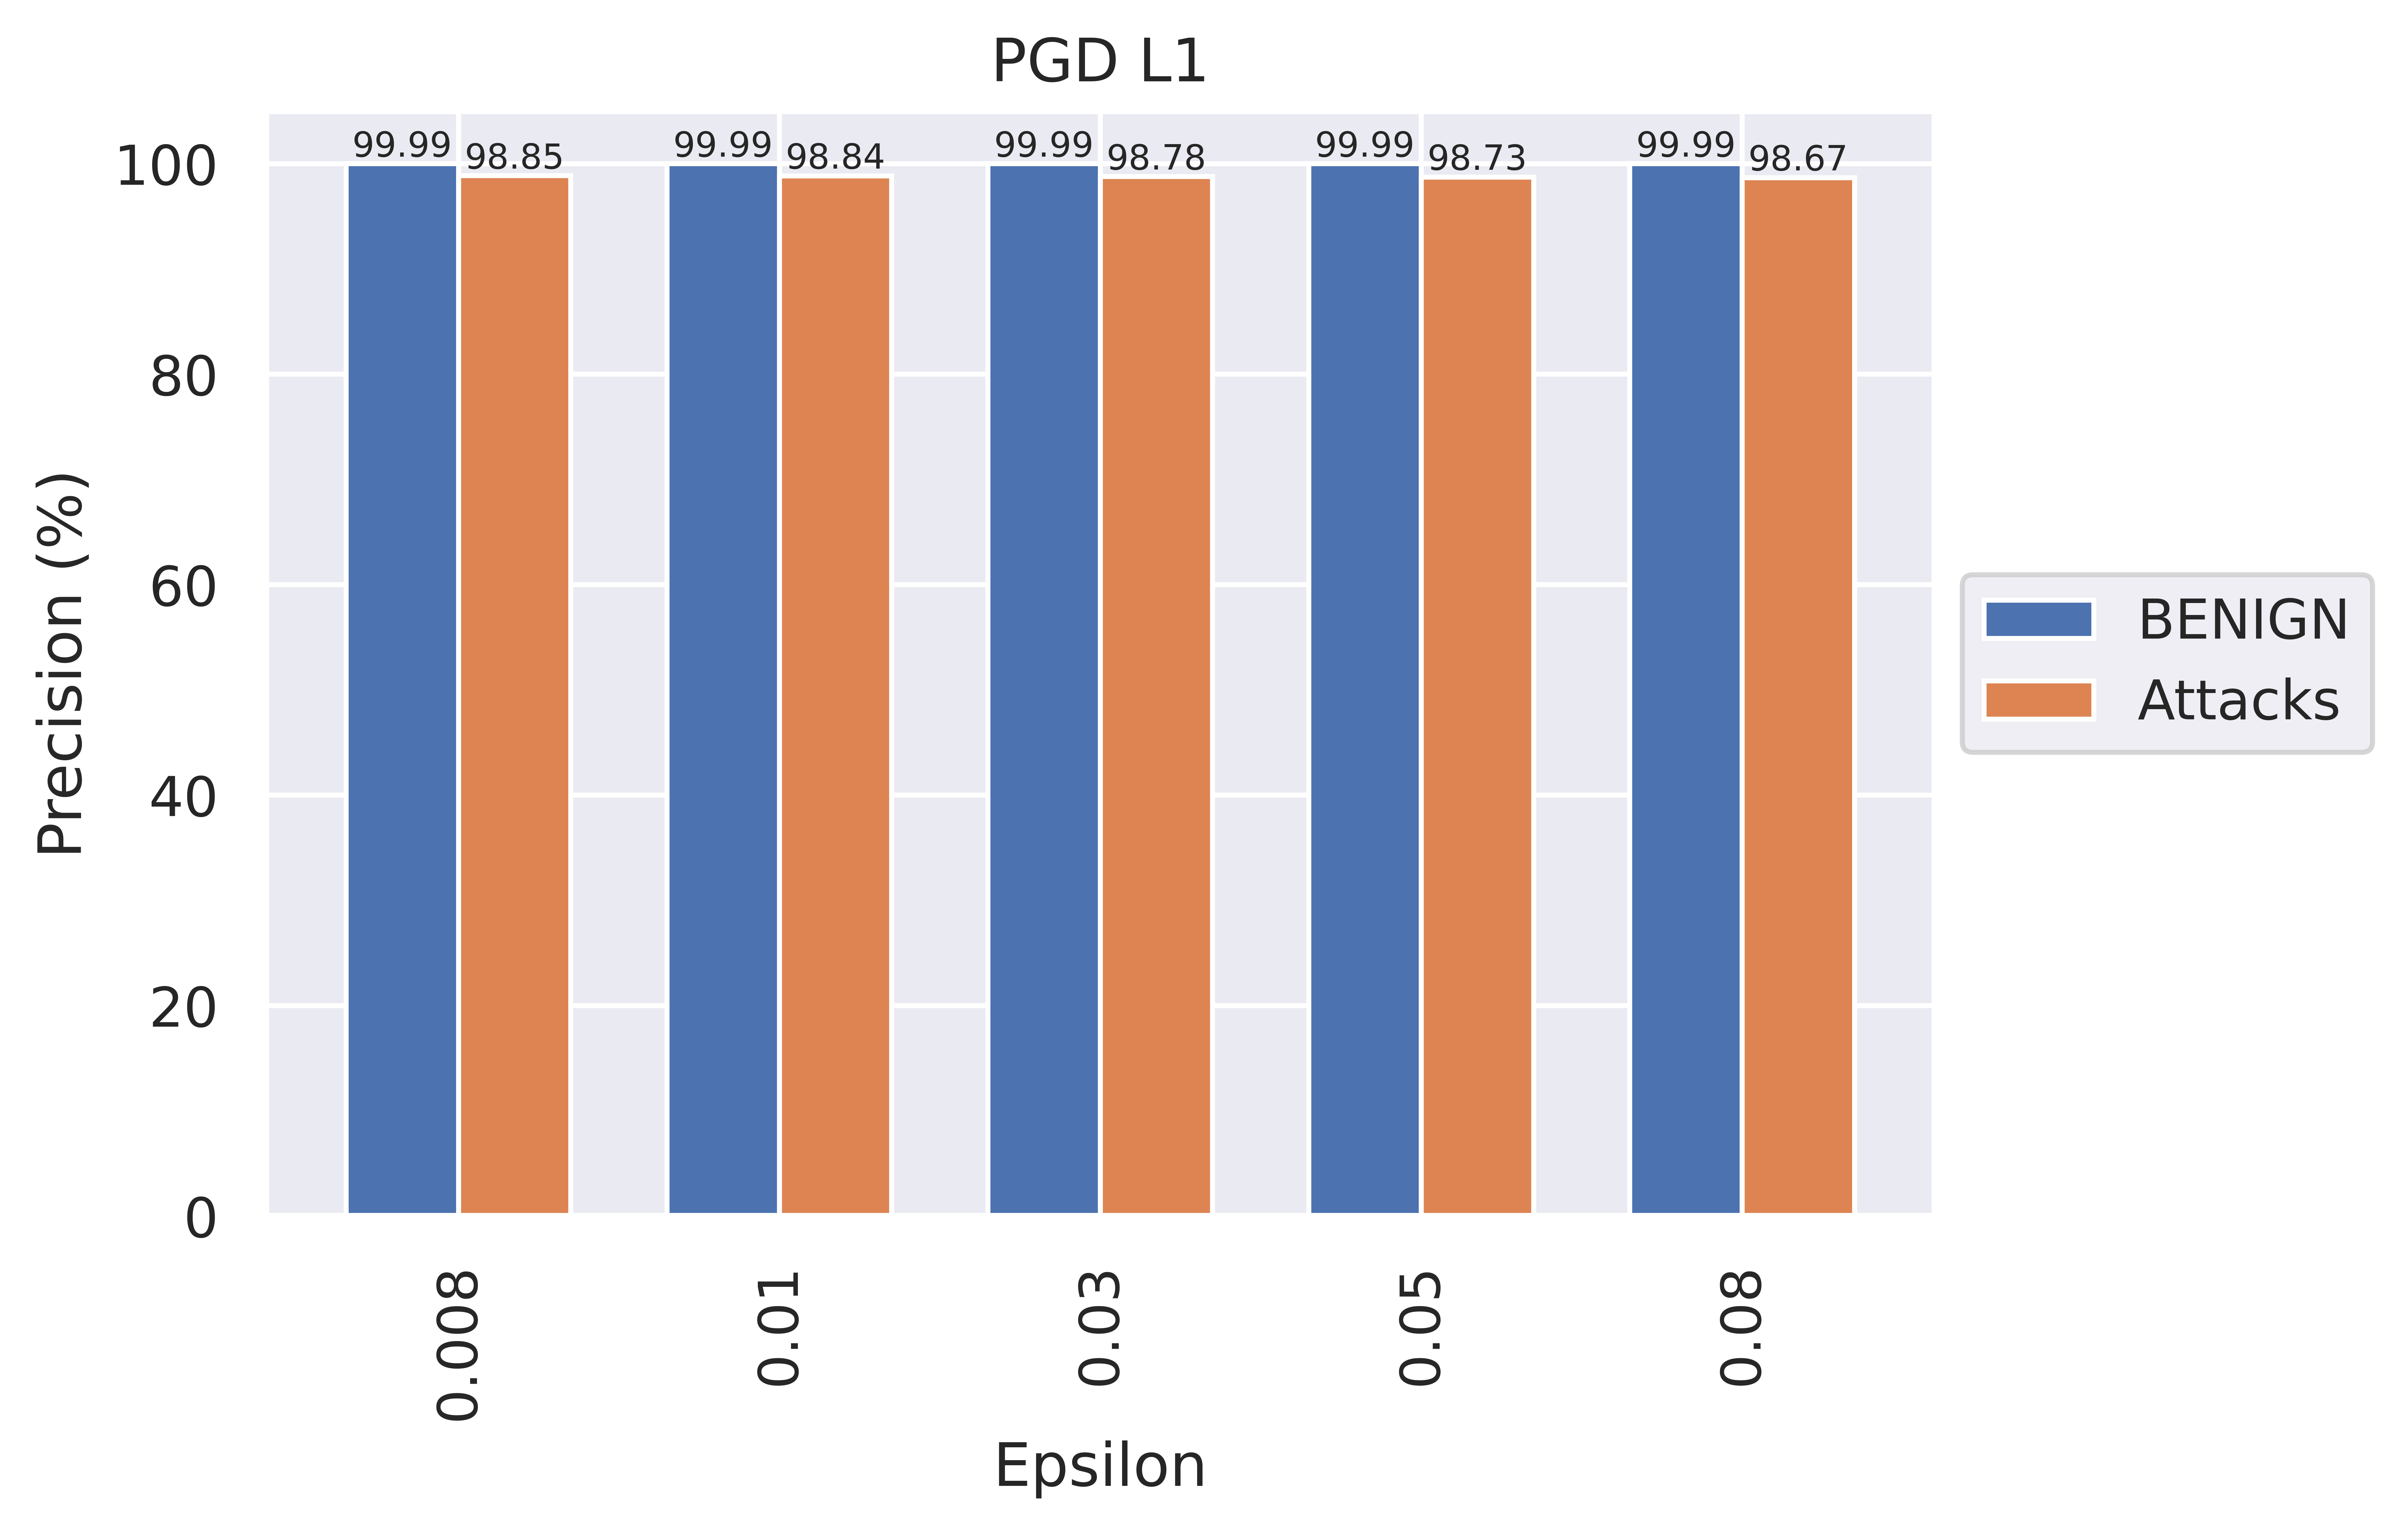
\includegraphics[width=\textwidth]{/home/wojtyla/Documentos/Artigo_2023/IJCNN_Suplementary/Figures//CIC_Clean_PGD L1_bin_paper.png}
			%caption{Figure}
			\label{fig:1}
		\end{subfigure}
		\hfill
		\begin{subfigure}[b]{0.45\textwidth}
			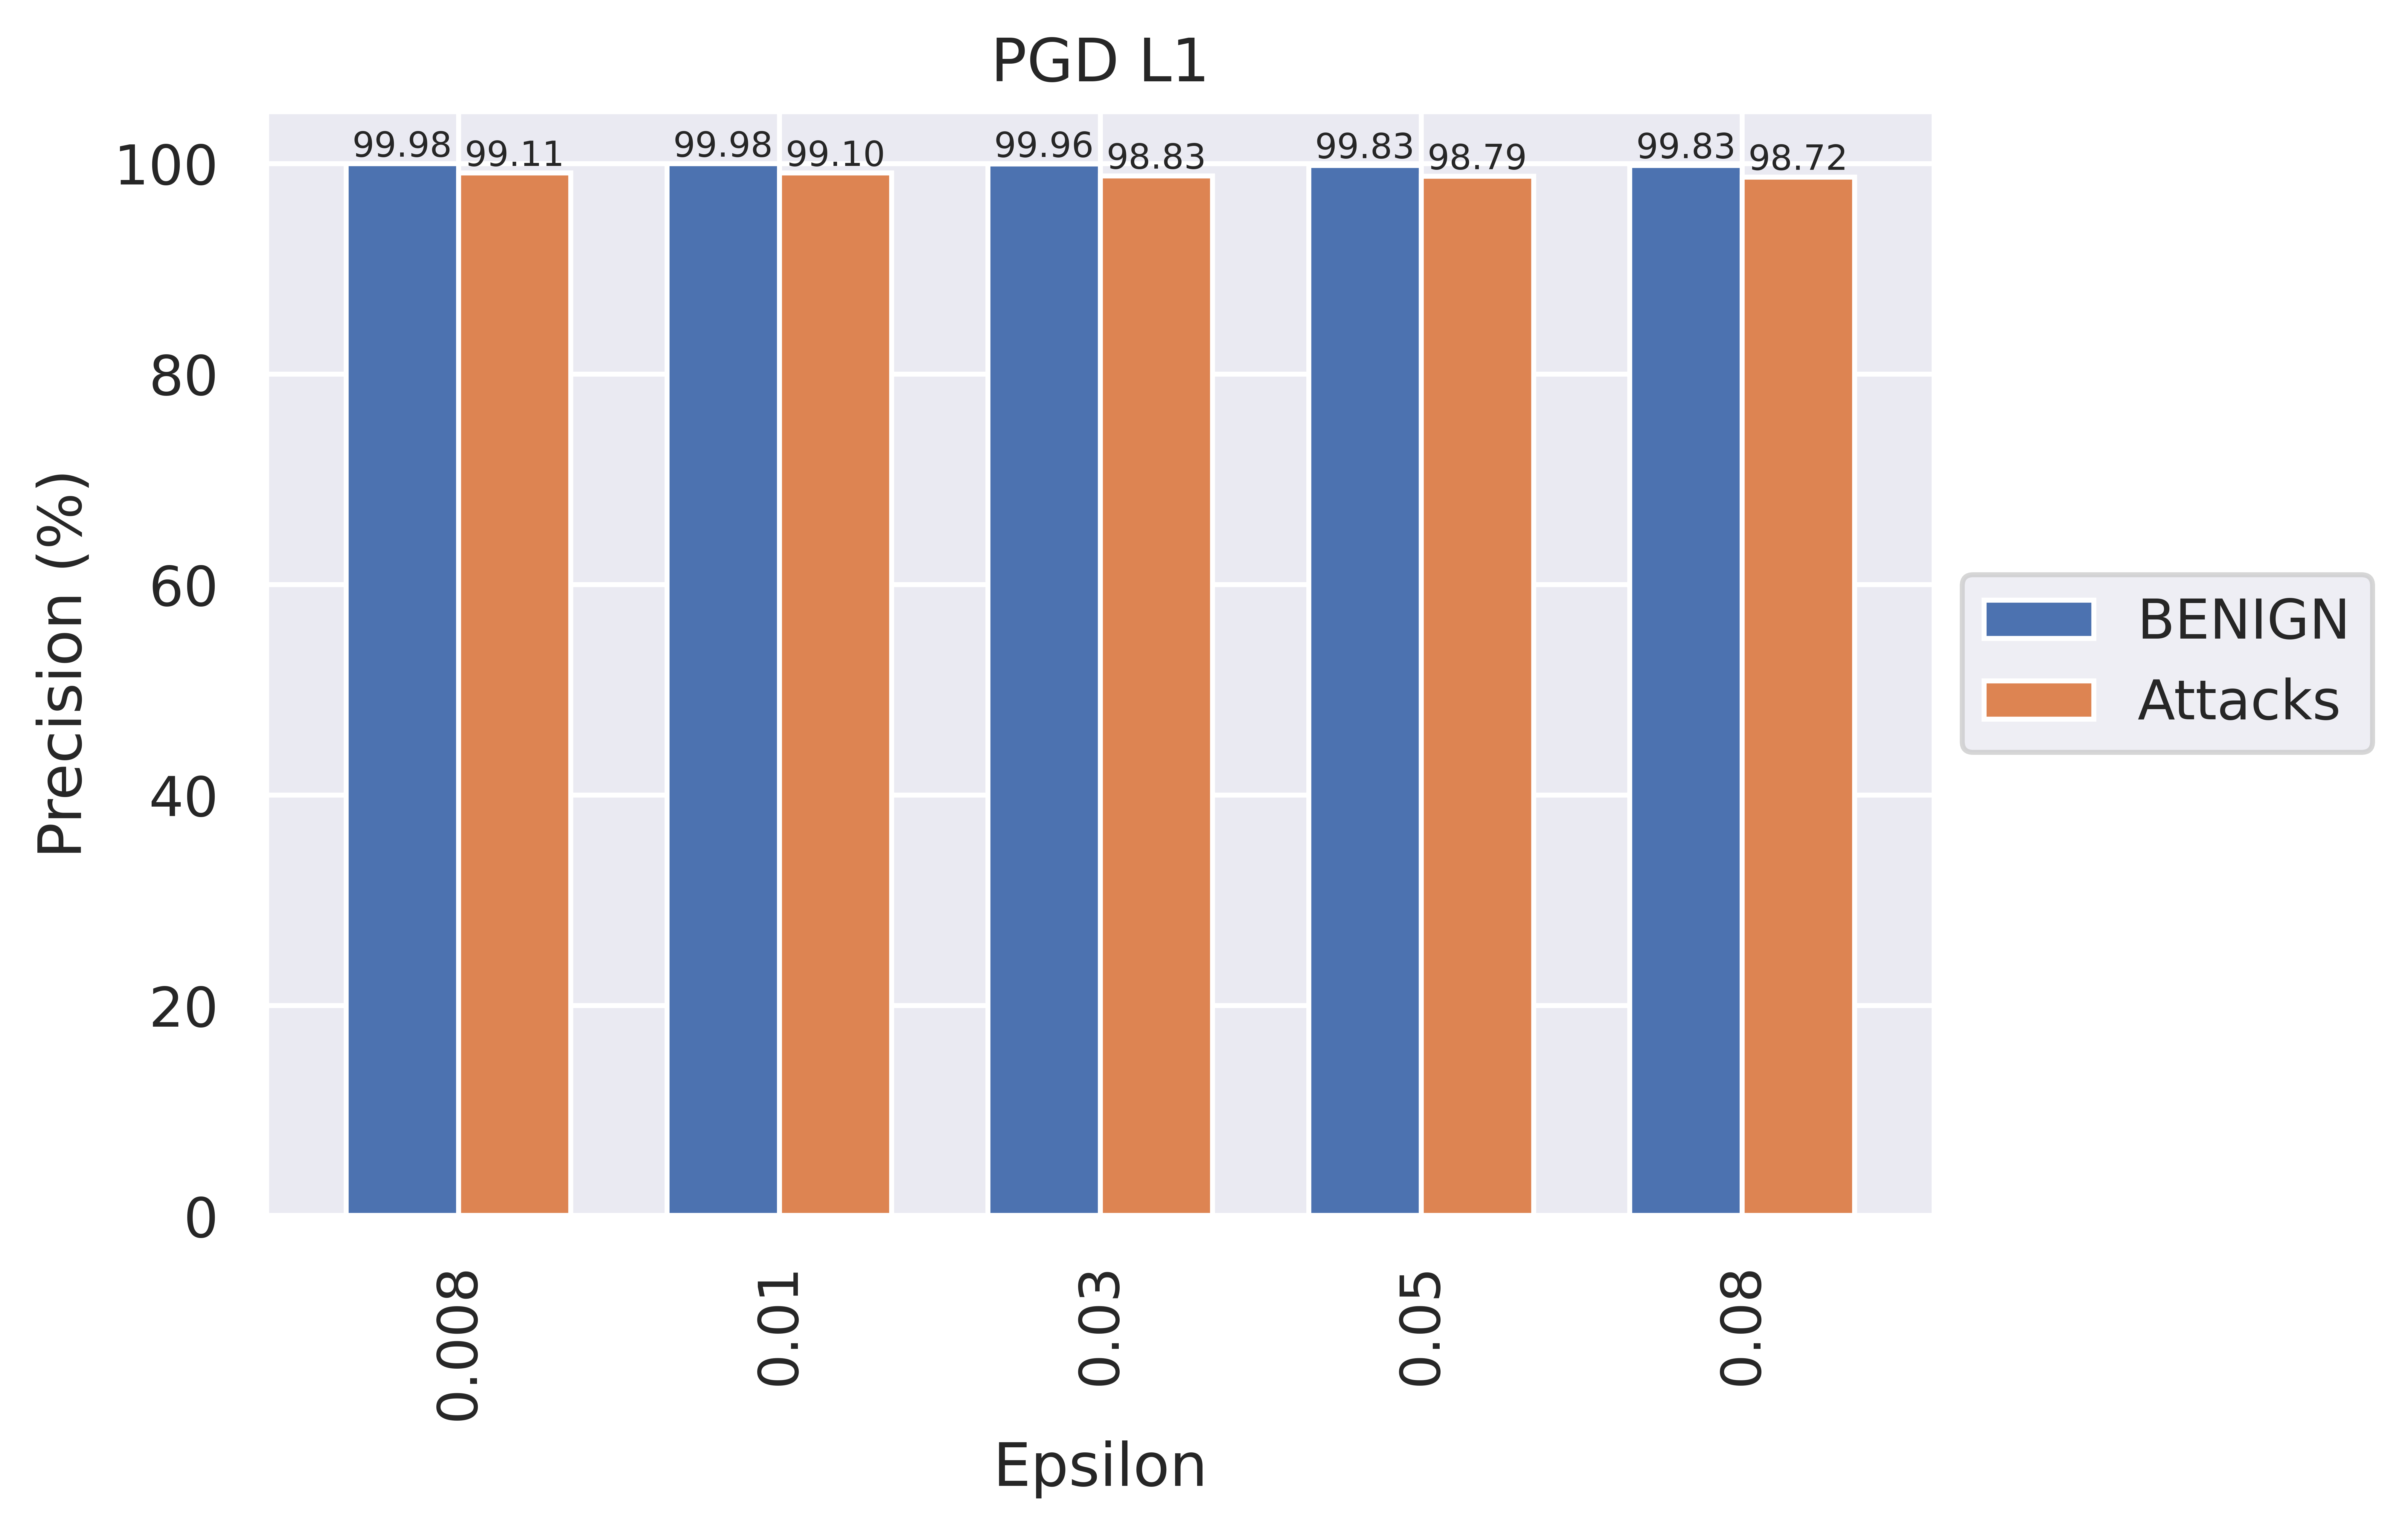
\includegraphics[width=\textwidth]{/home/wojtyla/Documentos/Artigo_2023/IJCNN_Suplementary/Figures//CIC_IDS_PGD L1_bin_paper.png}
			%caption{Figure}
			\label{fig:4}
		\end{subfigure}
		\vskip\baselineskip
		\begin{subfigure}[b]{0.45\textwidth}
			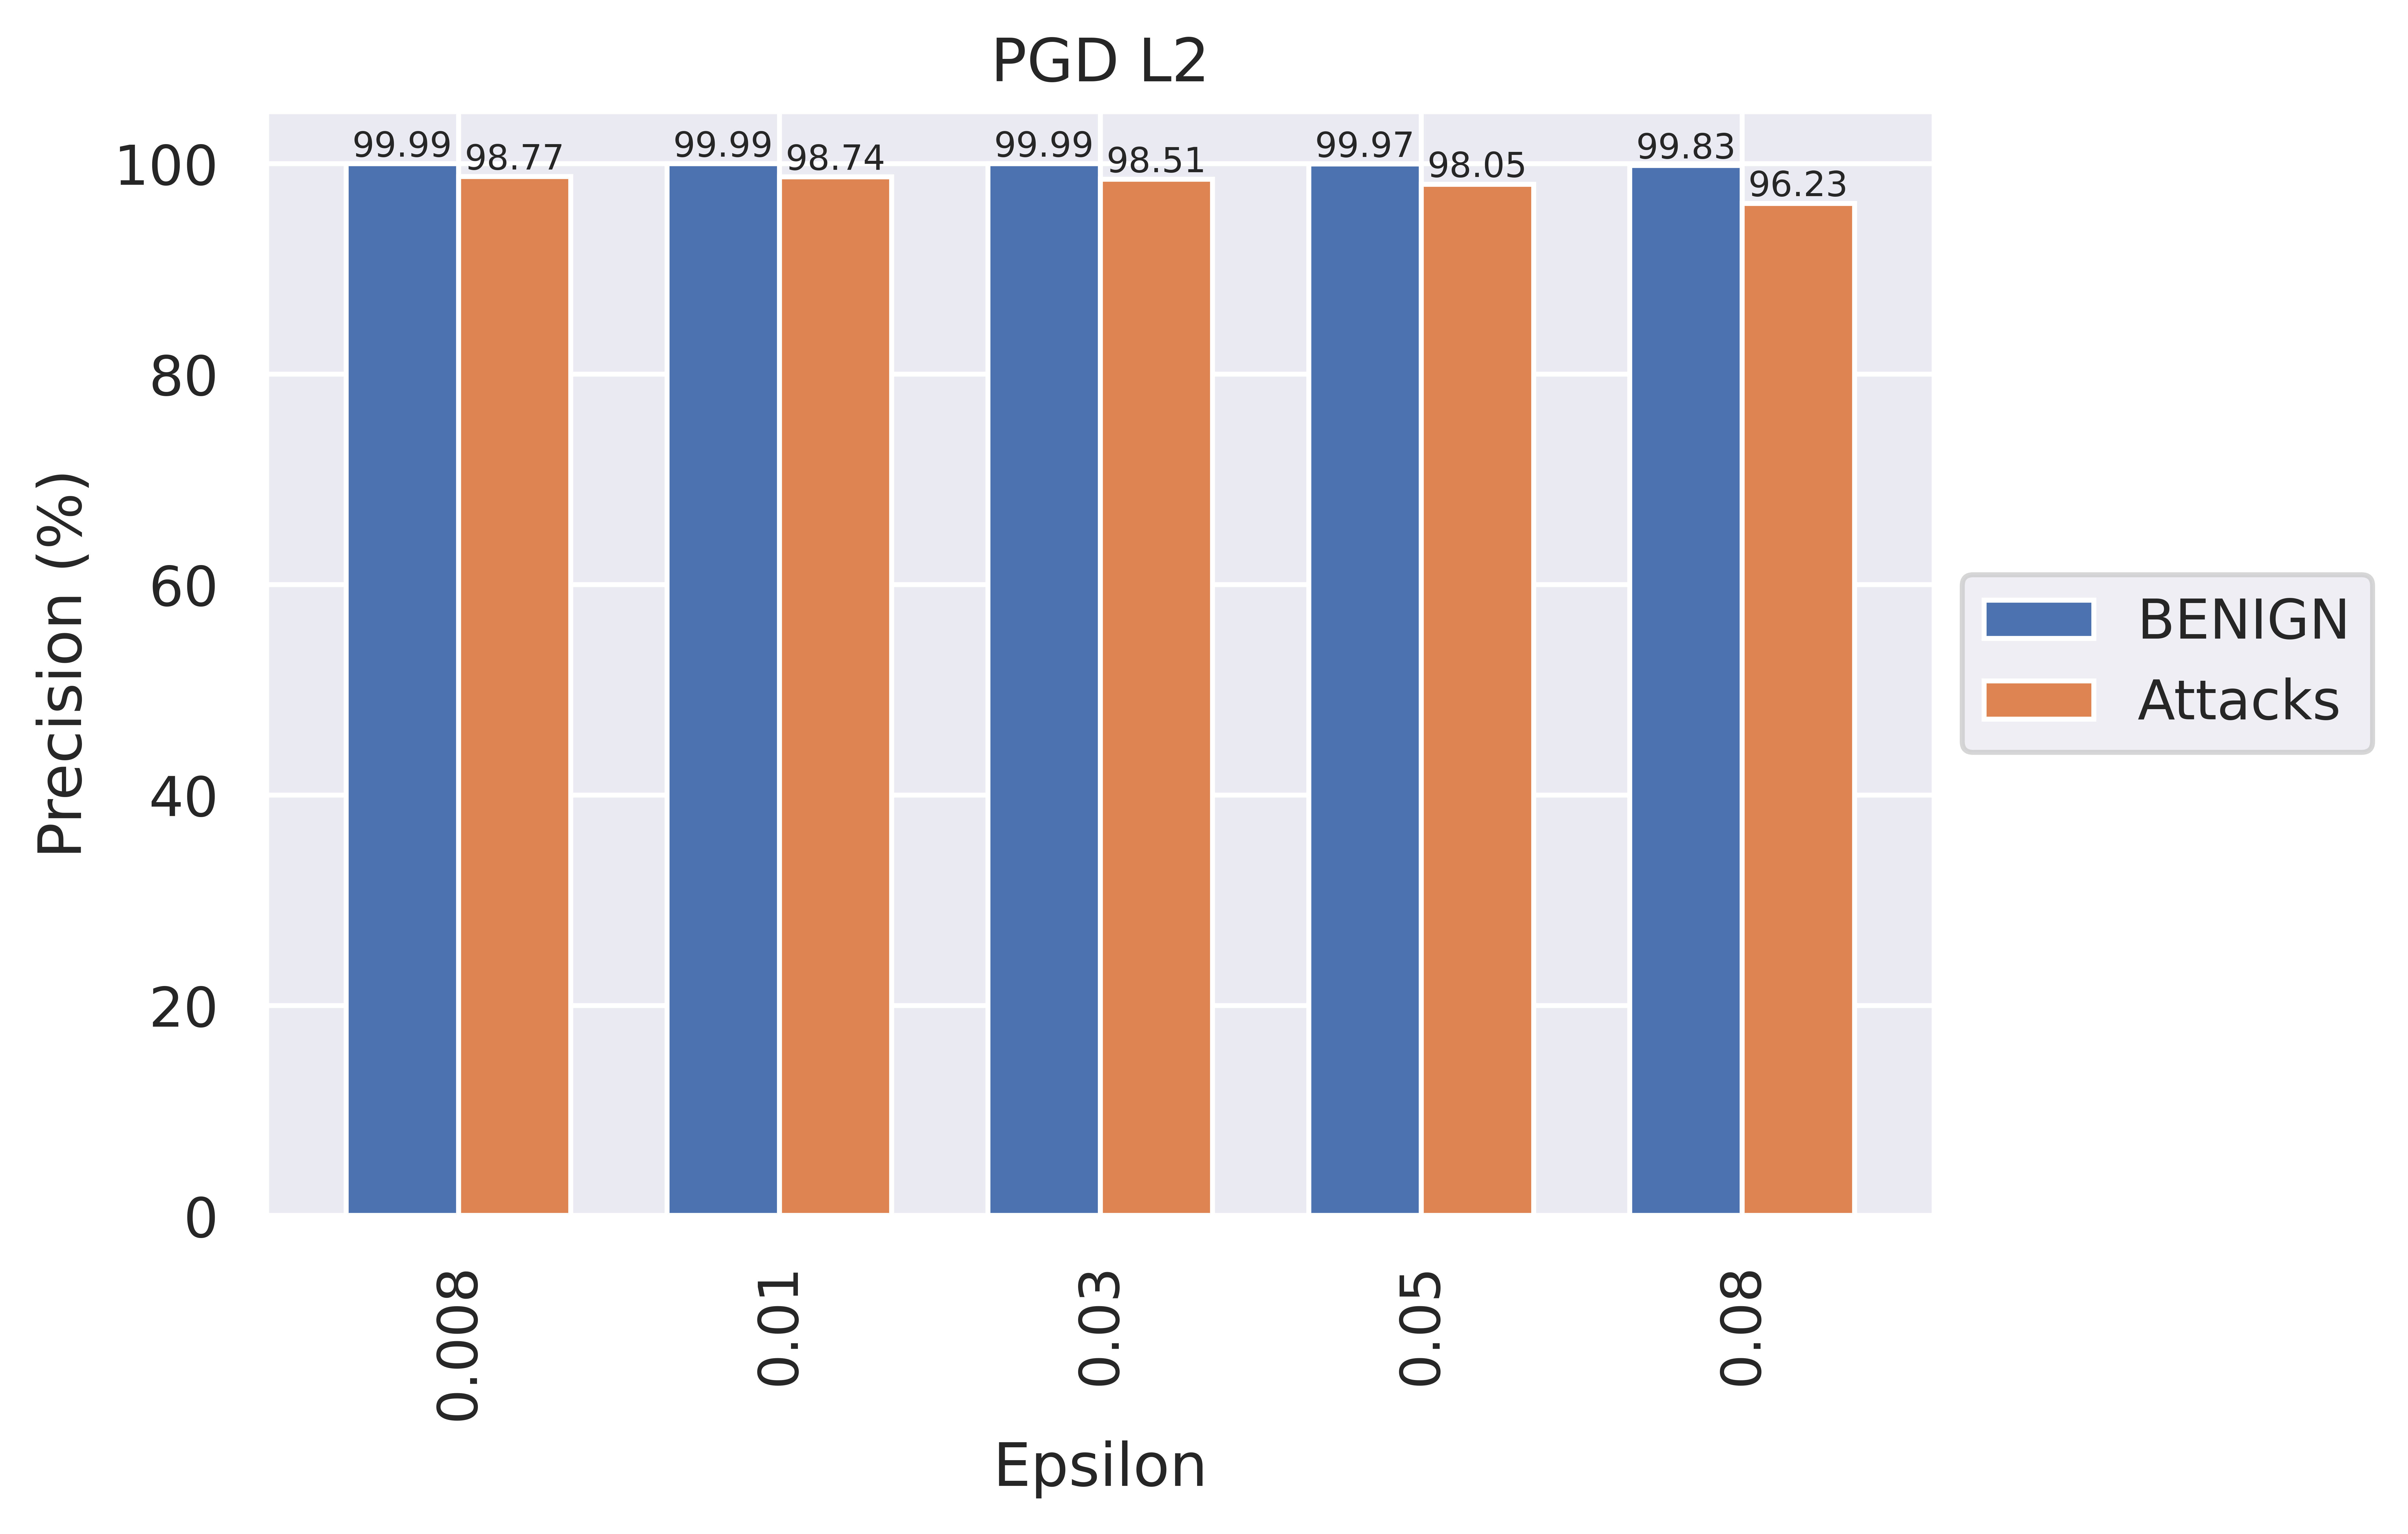
\includegraphics[width=\textwidth]{/home/wojtyla/Documentos/Artigo_2023/IJCNN_Suplementary/Figures//CIC_Clean_PGD L2_bin_paper.png}
			%caption{Figure}
			\label{fig:2}
		\end{subfigure}
		\hfill
		\begin{subfigure}[b]{0.45\textwidth}
			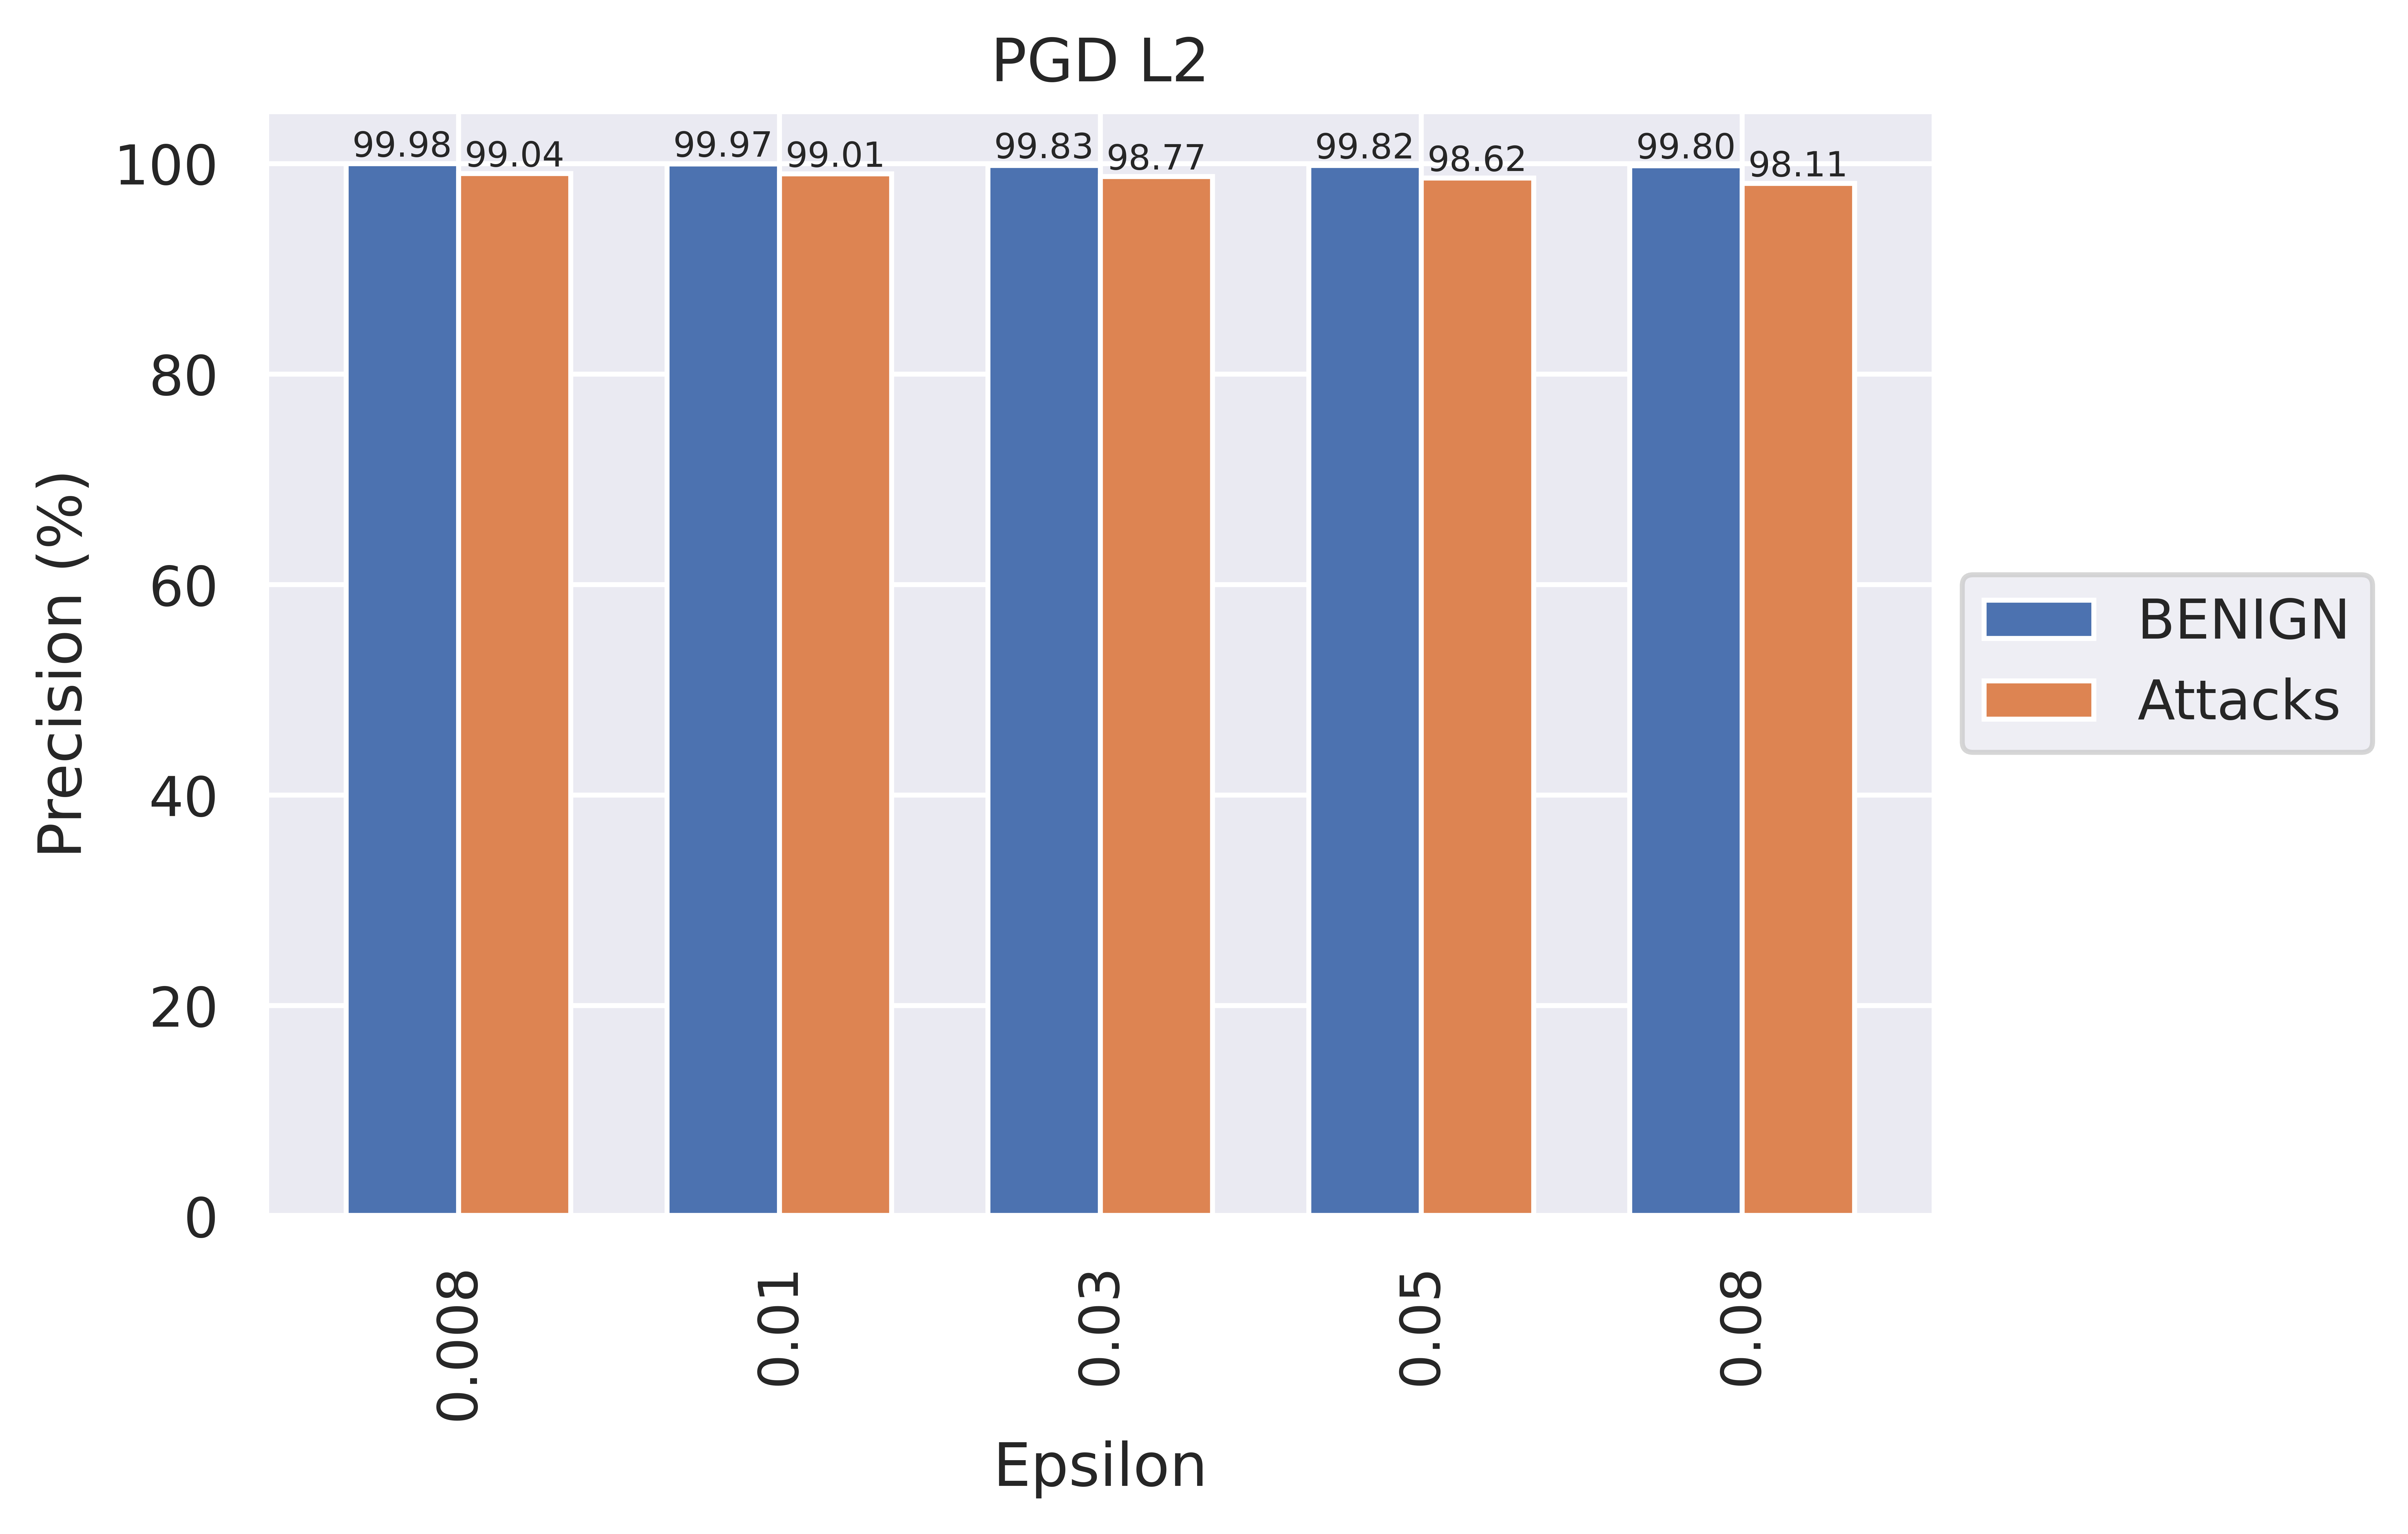
\includegraphics[width=\textwidth]{/home/wojtyla/Documentos/Artigo_2023/IJCNN_Suplementary/Figures///CIC_IDS_PGD L2_bin_paper.png}
			%caption{Figure}
			\label{fig:5}
		\end{subfigure}
		
		\vskip\baselineskip
		
		\begin{subfigure}[b]{0.45\textwidth}
			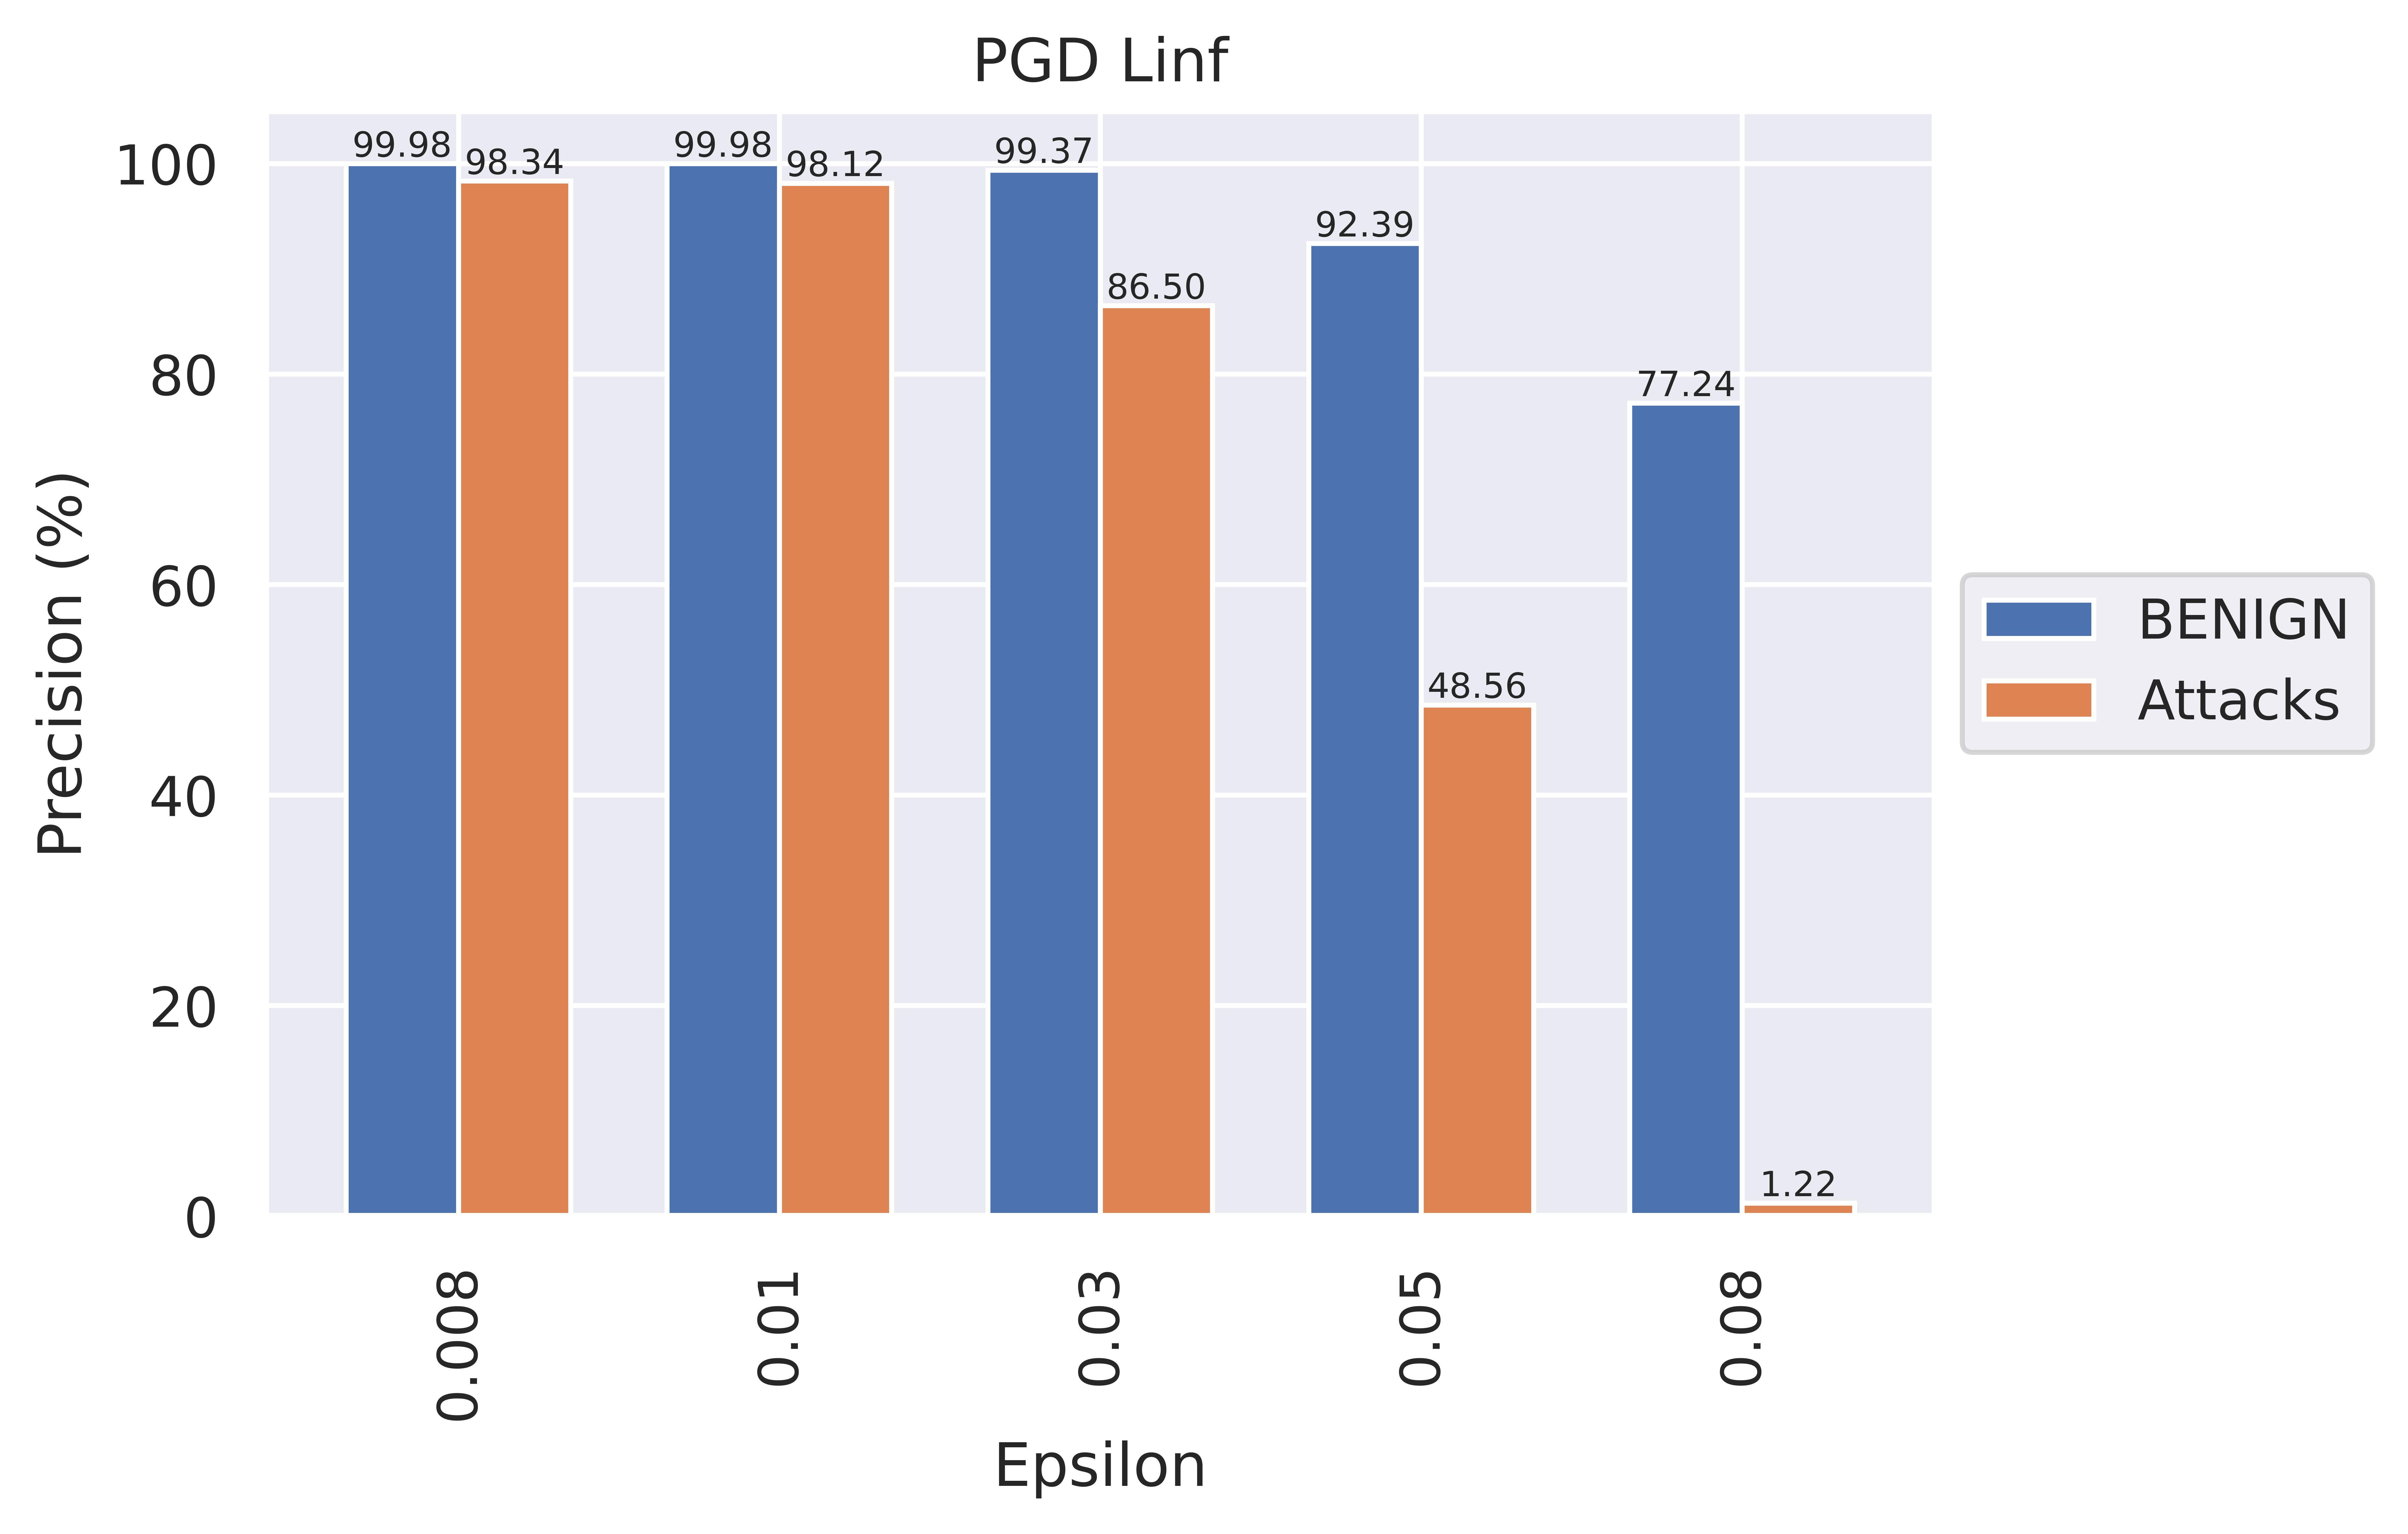
\includegraphics[width=\textwidth]{/home/wojtyla/Documentos/Artigo_2023/IJCNN_Suplementary/Figures//CIC_Clean_PGD Linf_bin_paper.png}
			%caption{Figure}
			\label{fig:3}
		\end{subfigure}			
		\hfill
		\begin{subfigure}[b]{0.45\textwidth}
			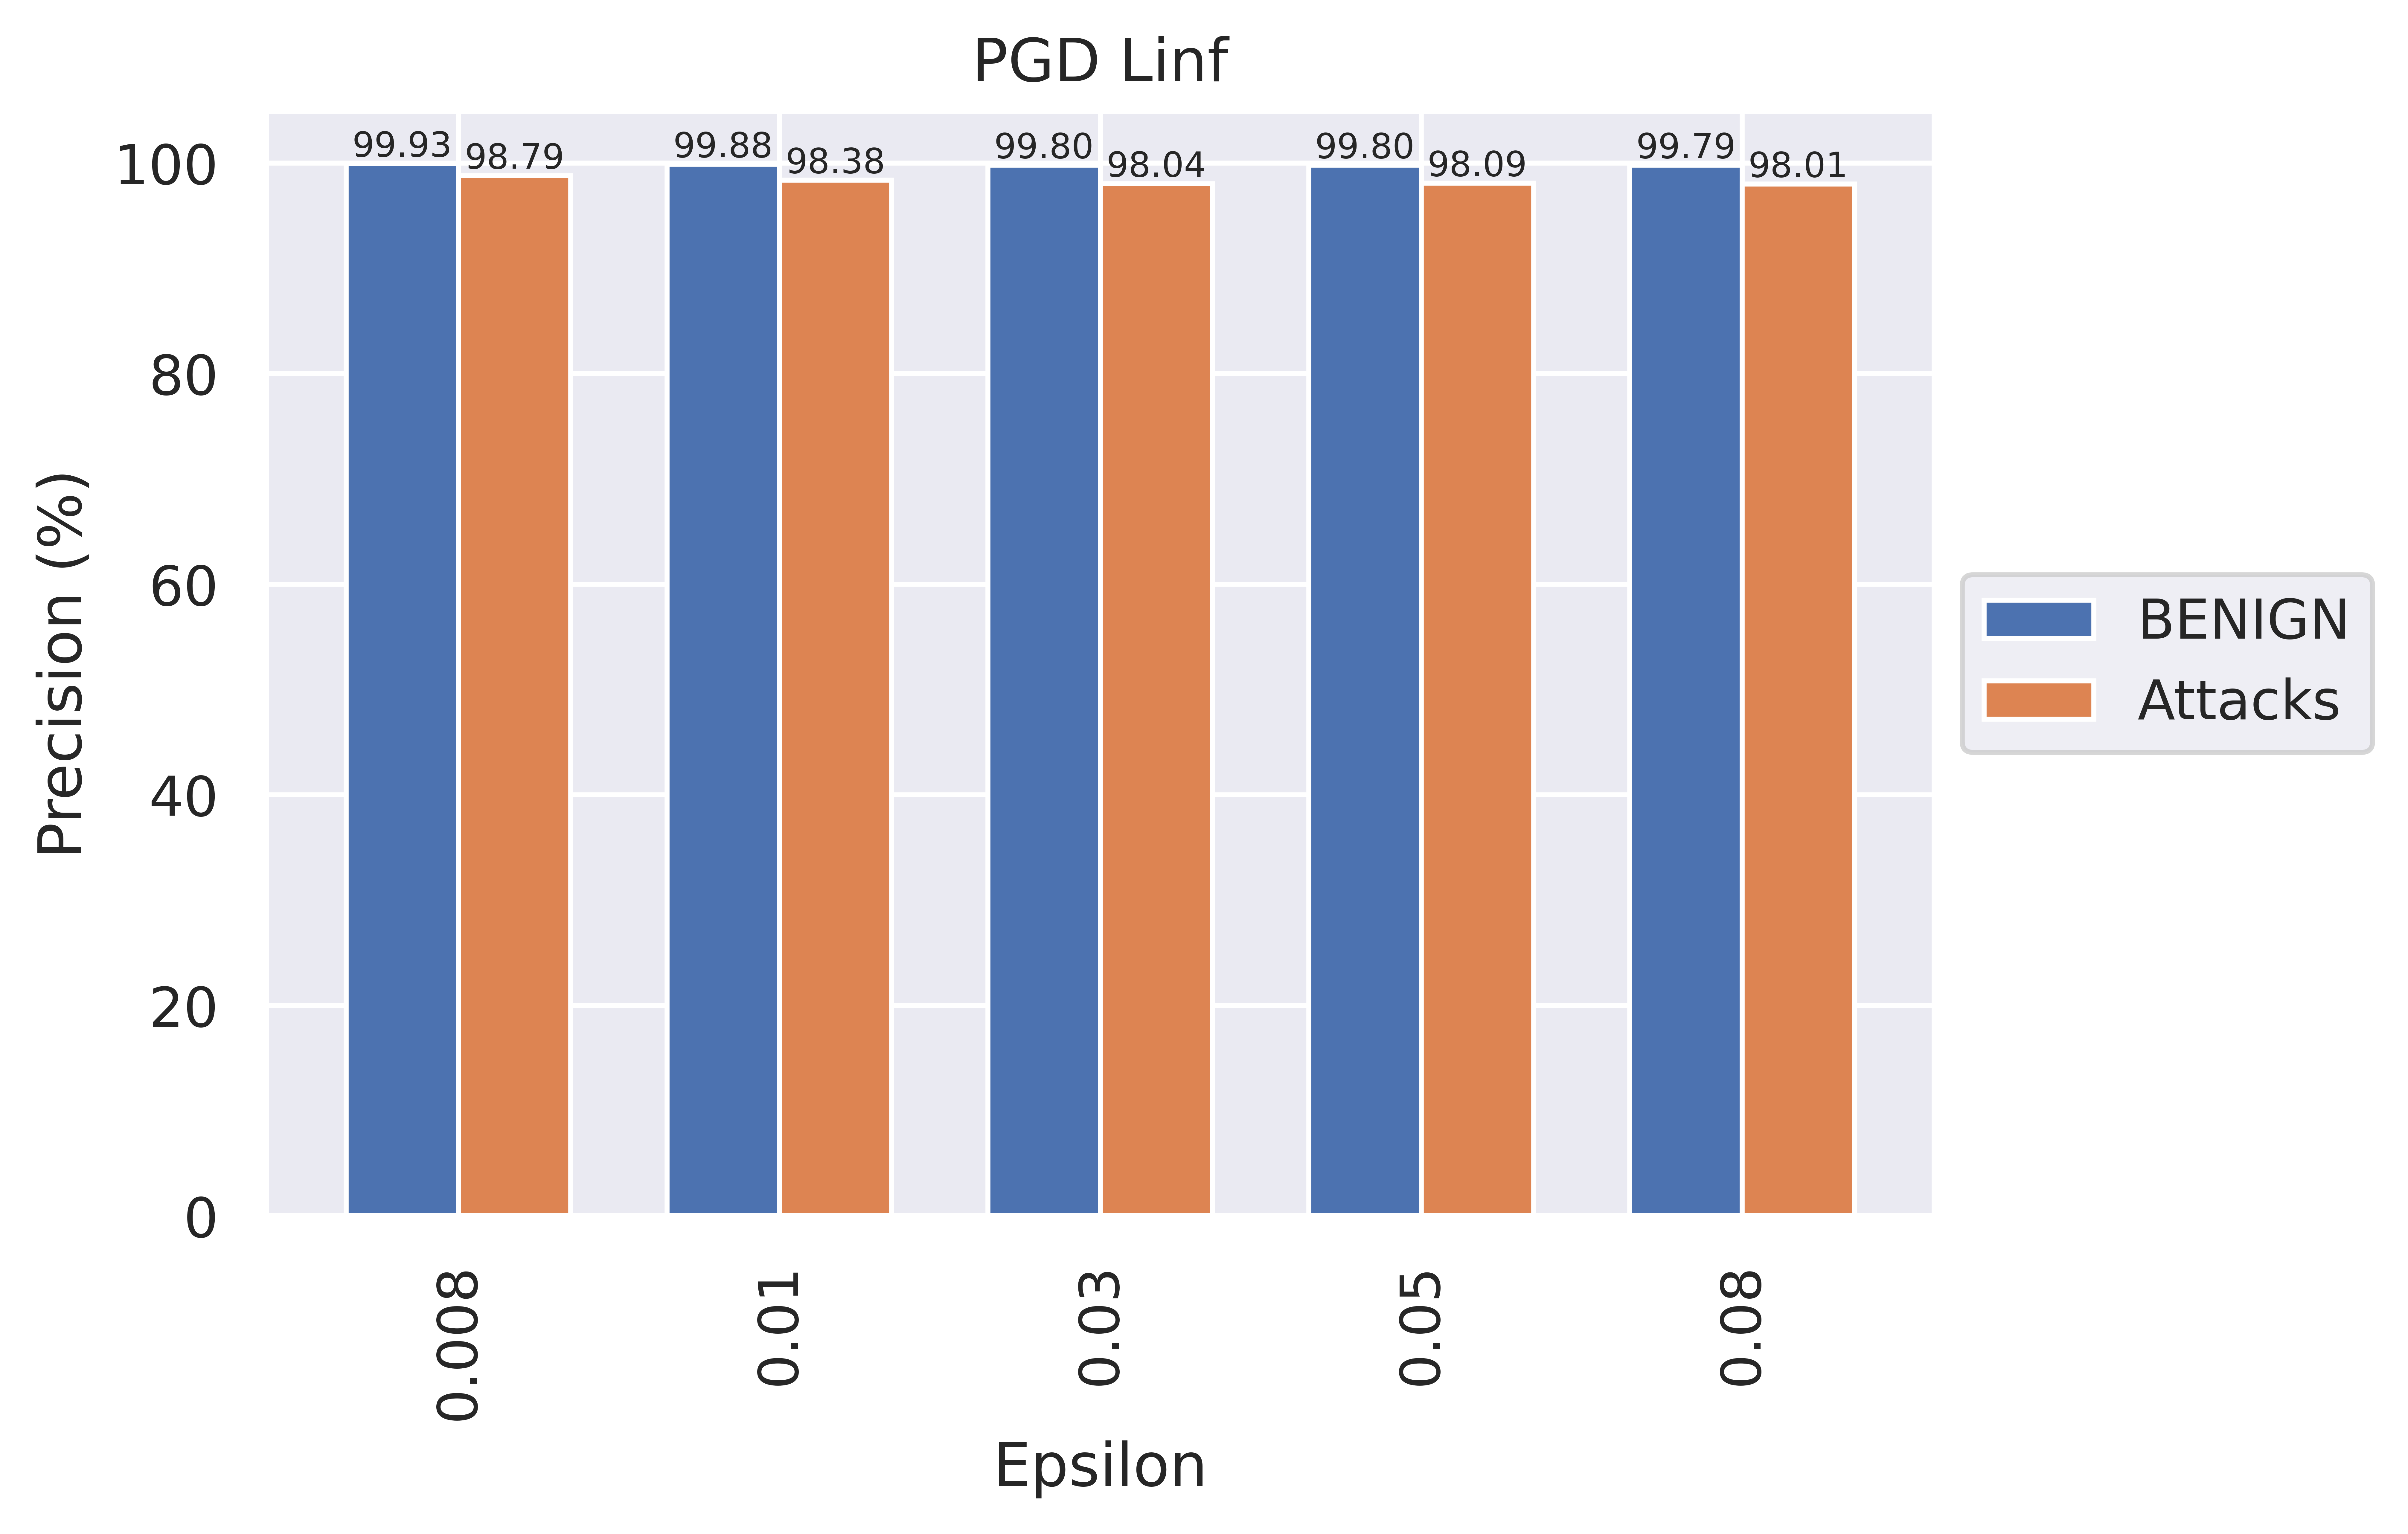
\includegraphics[width=\textwidth]{/home/wojtyla/Documentos/Artigo_2023/IJCNN_Suplementary/Figures///CIC_IDS_PGD Linf_bin_paper.png}
			%caption{Figure}
			\label{fig:6}
		\end{subfigure}
		\caption{Plots for PGD-100 attack on binary models with CIC IDS2017.Left:EnC model; Right:EnIDS model.}
		\label{fig:cic_pgd_bin}
	\end{figure}
	
	
	\begin{table}[h]
		\caption{PGD-100 attack against EnC and EnIDS for multiclass classification on the CIC IDS2017 dataset.}
		\small
		\setlength{\tabcolsep}{1pt}
		\centering
		\label{tab:cic_multi_pgd}
		\hspace*{-1.3cm}
		\begin{tabular}{|c|c|c|c|c|c|c|c|c|c|c|c|c|c|c|c|c|c|}
			\hline
			\multirow{3}{*}{\textbf{Type}} & \multirow{3}{*}{\textbf{Norm}} & \multirow{3}{*}{\textbf{Metrics}} & \multicolumn{15}{c|}{\textbf{Epsilon ($\epsilon$)}
			} \\
			\cline{4-18}
			&  &  & \multicolumn{3}{c|}{\textbf{0.008}} & \multicolumn{3}{c|}{\textbf{0.01}} & \multicolumn{3}{c|}{\textbf{0.03}} & \multicolumn{3}{c|}{\textbf{0.05}} & \multicolumn{3}{c|}{\textbf{0.08}}
			\\
			\cline{4-18}
			&  &  & \textbf{\textsl{Benign}} & \textbf{\textsl{DOS}} & \textbf{\textsl{DDOS}} & \textbf{\textsl{Benign}} & \textbf{\textsl{DOS}} & \textbf{\textsl{DDOS}} & \textbf{\textsl{Benign}} & \textbf{\textsl{DOS}} & \textbf{\textsl{DDOS}} & \textbf{\textsl{Benign}} & \textbf{\textsl{DOS}} & \textbf{\textsl{DDOS}} & \textbf{\textsl{Benign}} & \textbf{\textsl{DOS}} & \textbf{\textsl{DDOS}}
			\\
			\hline
			\multirow{9}{*}
			{EnC} & \multirow{3}{*}{\( \ell_1 \)} & Precision & 99.98 & 99.30 & 99.99 & 99.97 & 99.30 & 99.99 & 99.97 & 99.26 & 99.99 & 99.97 & 99.24 & 99.99 & 99.97 & 99.21 & 99.99
			\\
			
			&  & Recall & 99.44 & 99.75 & 99.99 & 99.44 & 99.75 & 99.99 & 99.41 & 99.75 & 99.99 & 99.38 & 99.75 & 99.99 & 99.30 & 99.75 & 99.99
			\\
			
			&  & ROC-AUC & 99.98 & 100.00 & 100.00 & 99.98 & 100.00 & 100.00 & 99.98 & 100.00 & 100.00 & 99.98 & 100.00 & 100.00 & 99.98 & 100.00 & 100.00
			\\
			\cline{2-18}
			& \multirow{3}{*}{\( \ell_2 \)} & Precision & 99.97 & 99.24 & 99.99 & 99.97 & 99.24 & 99.99 & 99.96 & 99.07 & 99.99 & 99.95 & 98.83 & 99.99 & 99.81 & 98.17 & 99.99
			\\
			
			&  & Recall & 99.41 & 99.75 & 99.99 & 99.39 & 99.75 & 99.99 & 99.17 & 99.72 & 99.97 & 98.83 & 99.64 & 99.94 & 98.23 & 99.40 & 99.83
			\\
			
			&  & ROC-AUC & 99.98 & 100.00 & 100.00 & 99.98 & 100.00 & 100.00 & 99.97 & 100.00 & 100.00 & 99.95 & 99.99 & 100.00 & 99.87 & 99.94 & 100.00
			\\
			\cline{2-18}
			& \multirow{3}{*}{\( \ell_\infty \)} & Precision & 99.96 & 98.94 & 99.99 & 99.95 & 98.74 & 99.99 & 99.55 & 90.49 & 99.96 & 97.21 & 63.13 & 99.80 & 85.39 & 15.56 & 94.45
			\\
			
			&  & Recall & 99.05 & 99.69 & 99.94 & 98.92 & 99.64 & 99.93 & 95.67 & 96.84 & 93.84 & 84.83 & 80.39 & 81.14 & 62.34 & 21.91 & 76.96
			\\
			
			&  & ROC-AUC & 99.96 & 99.99 & 100.00 & 99.95 & 99.99 & 100.00 & 99.38 & 99.00 & 99.99 & 94.16 & 96.12 & 99.37 & 59.82 & 63.23 & 90.39
			\\
			\hline
			\multirow{9}{*}
			{EnIDS} & \multirow{3}{*}{\( \ell_1 \)} & Precision & \cellcolor{yellow!50}99.99 & 98.95 & 99.94 & \cellcolor{yellow!50}99.99 & 98.95 & 99.94 & \cellcolor{yellow!50}99.99 & 98.94 & 99.94 & \cellcolor{yellow!50}99.99 & 98.91 & 99.94 & \cellcolor{yellow!50}99.99 & 98.87 & 99.93
			\\
			
			&  & Recall & \cellcolor{yellow!50}97.81 & \cellcolor{yellow!50}99.93 & \cellcolor{yellow!50}100.00 & 97.79 & \cellcolor{yellow!50}99.93 & \cellcolor{yellow!50}100.00 & 97.56 & \cellcolor{yellow!50}99.91 & \cellcolor{yellow!50}100.00 & 97.30 & \cellcolor{yellow!50}99.91 & 99.99 & 97.06 & \cellcolor{yellow!50}99.90 & 99.95
			\\
			
			&  & ROC-AUC & 99.97 & \cellcolor{blue!20}100.00 & \cellcolor{blue!20}100.00 & 99.97 & \cellcolor{blue!20}100.00 & \cellcolor{blue!20}100.00 & 99.96 & \cellcolor{blue!20}100.00 & \cellcolor{blue!20}100.00 & 99.95 & \cellcolor{blue!20}100.00 & \cellcolor{blue!20}100.00 & 99.92 & \cellcolor{blue!20}100.00 & \cellcolor{blue!20}100.00
			\\
			\cline{2-18}
			& \multirow{3}{*}{\( \ell_2 \)} & Precision & \cellcolor{yellow!50}99.99 & 98.94 & 99.94 & \cellcolor{yellow!50}99.99 & 98.93 & 99.93 & \cellcolor{yellow!50}99.99 & 98.75 & 99.93 & \cellcolor{yellow!50}99.99 & 98.57 & 99.93 & \cellcolor{yellow!50}99.98 & \cellcolor{yellow!50}98.29 & 99.93
			\\
			
			&  & Recall & 97.62 & \cellcolor{yellow!50}99.92 & \cellcolor{yellow!50}100.00 & 97.55 & \cellcolor{yellow!50}99.91 & \cellcolor{yellow!50}100.00 & 96.72 & \cellcolor{yellow!50}99.89 & 99.96 & 96.04 & \cellcolor{yellow!50}99.86 & \cellcolor{yellow!50}99.98 & 96.06 & \cellcolor{yellow!50}99.85 & \cellcolor{yellow!50}99.99
			\\
			
			&  & ROC-AUC & 99.96 & \cellcolor{blue!20}100.00 & \cellcolor{blue!20}100.00 & 99.95 & \cellcolor{blue!20}100.00 & \cellcolor{blue!20}100.00 & 99.64 & 99.99 & \cellcolor{blue!20}100.00 & 99.22 & 99.98 & \cellcolor{blue!20}100.00 & 99.76 & 99.98 & \cellcolor{blue!20}100.00
			\\
			\cline{2-18}
			& \multirow{3}{*}{\( \ell_\infty \)} & Precision & \cellcolor{yellow!50}99.99 & 98.66 & 99.92 & \cellcolor{yellow!50}99.99 & 98.60 & 99.93 & \cellcolor{yellow!50}99.97 & \cellcolor{yellow!50}97.49 & \cellcolor{yellow!50}99.92 & \cellcolor{yellow!50}99.94 & \cellcolor{yellow!50}94.87 & \cellcolor{yellow!50}99.91 & \cellcolor{yellow!50}99.73 & \cellcolor{yellow!50}83.52 & \cellcolor{yellow!50}99.91
			\\
			
			&  & Recall & 96.49 & \cellcolor{yellow!50}99.85 & \cellcolor{yellow!50}99.95 & 96.25 & \cellcolor{yellow!50}99.84 & 99.97 & \cellcolor{yellow!50}96.20 & \cellcolor{yellow!50}99.75 & \cellcolor{yellow!50}100.00 & \cellcolor{yellow!50}95.53 & \cellcolor{yellow!50}99.45 & \cellcolor{yellow!50}99.98 & \cellcolor{yellow!50}92.63 & \cellcolor{yellow!50}97.73 & \cellcolor{yellow!50}99.97
			\\
			
			&  & ROC-AUC & 99.75 & 99.99 & 100.00 & 99.47 & 99.99 & 100.00 & 99.68 & \cellcolor{yellow!50}99.98 & \cellcolor{yellow!50}100.00 & \cellcolor{yellow!50}99.59 & \cellcolor{yellow!50}99.93 & \cellcolor{yellow!50}100.00 & \cellcolor{yellow!50}99.03 & \cellcolor{yellow!50}99.63 & \cellcolor{yellow!50}100.00
			\\
			\hline
		\end{tabular}
	\end{table}
	
	
	\begin{figure}[H]
		\centering
		\begin{subfigure}[b]{0.45\textwidth}
			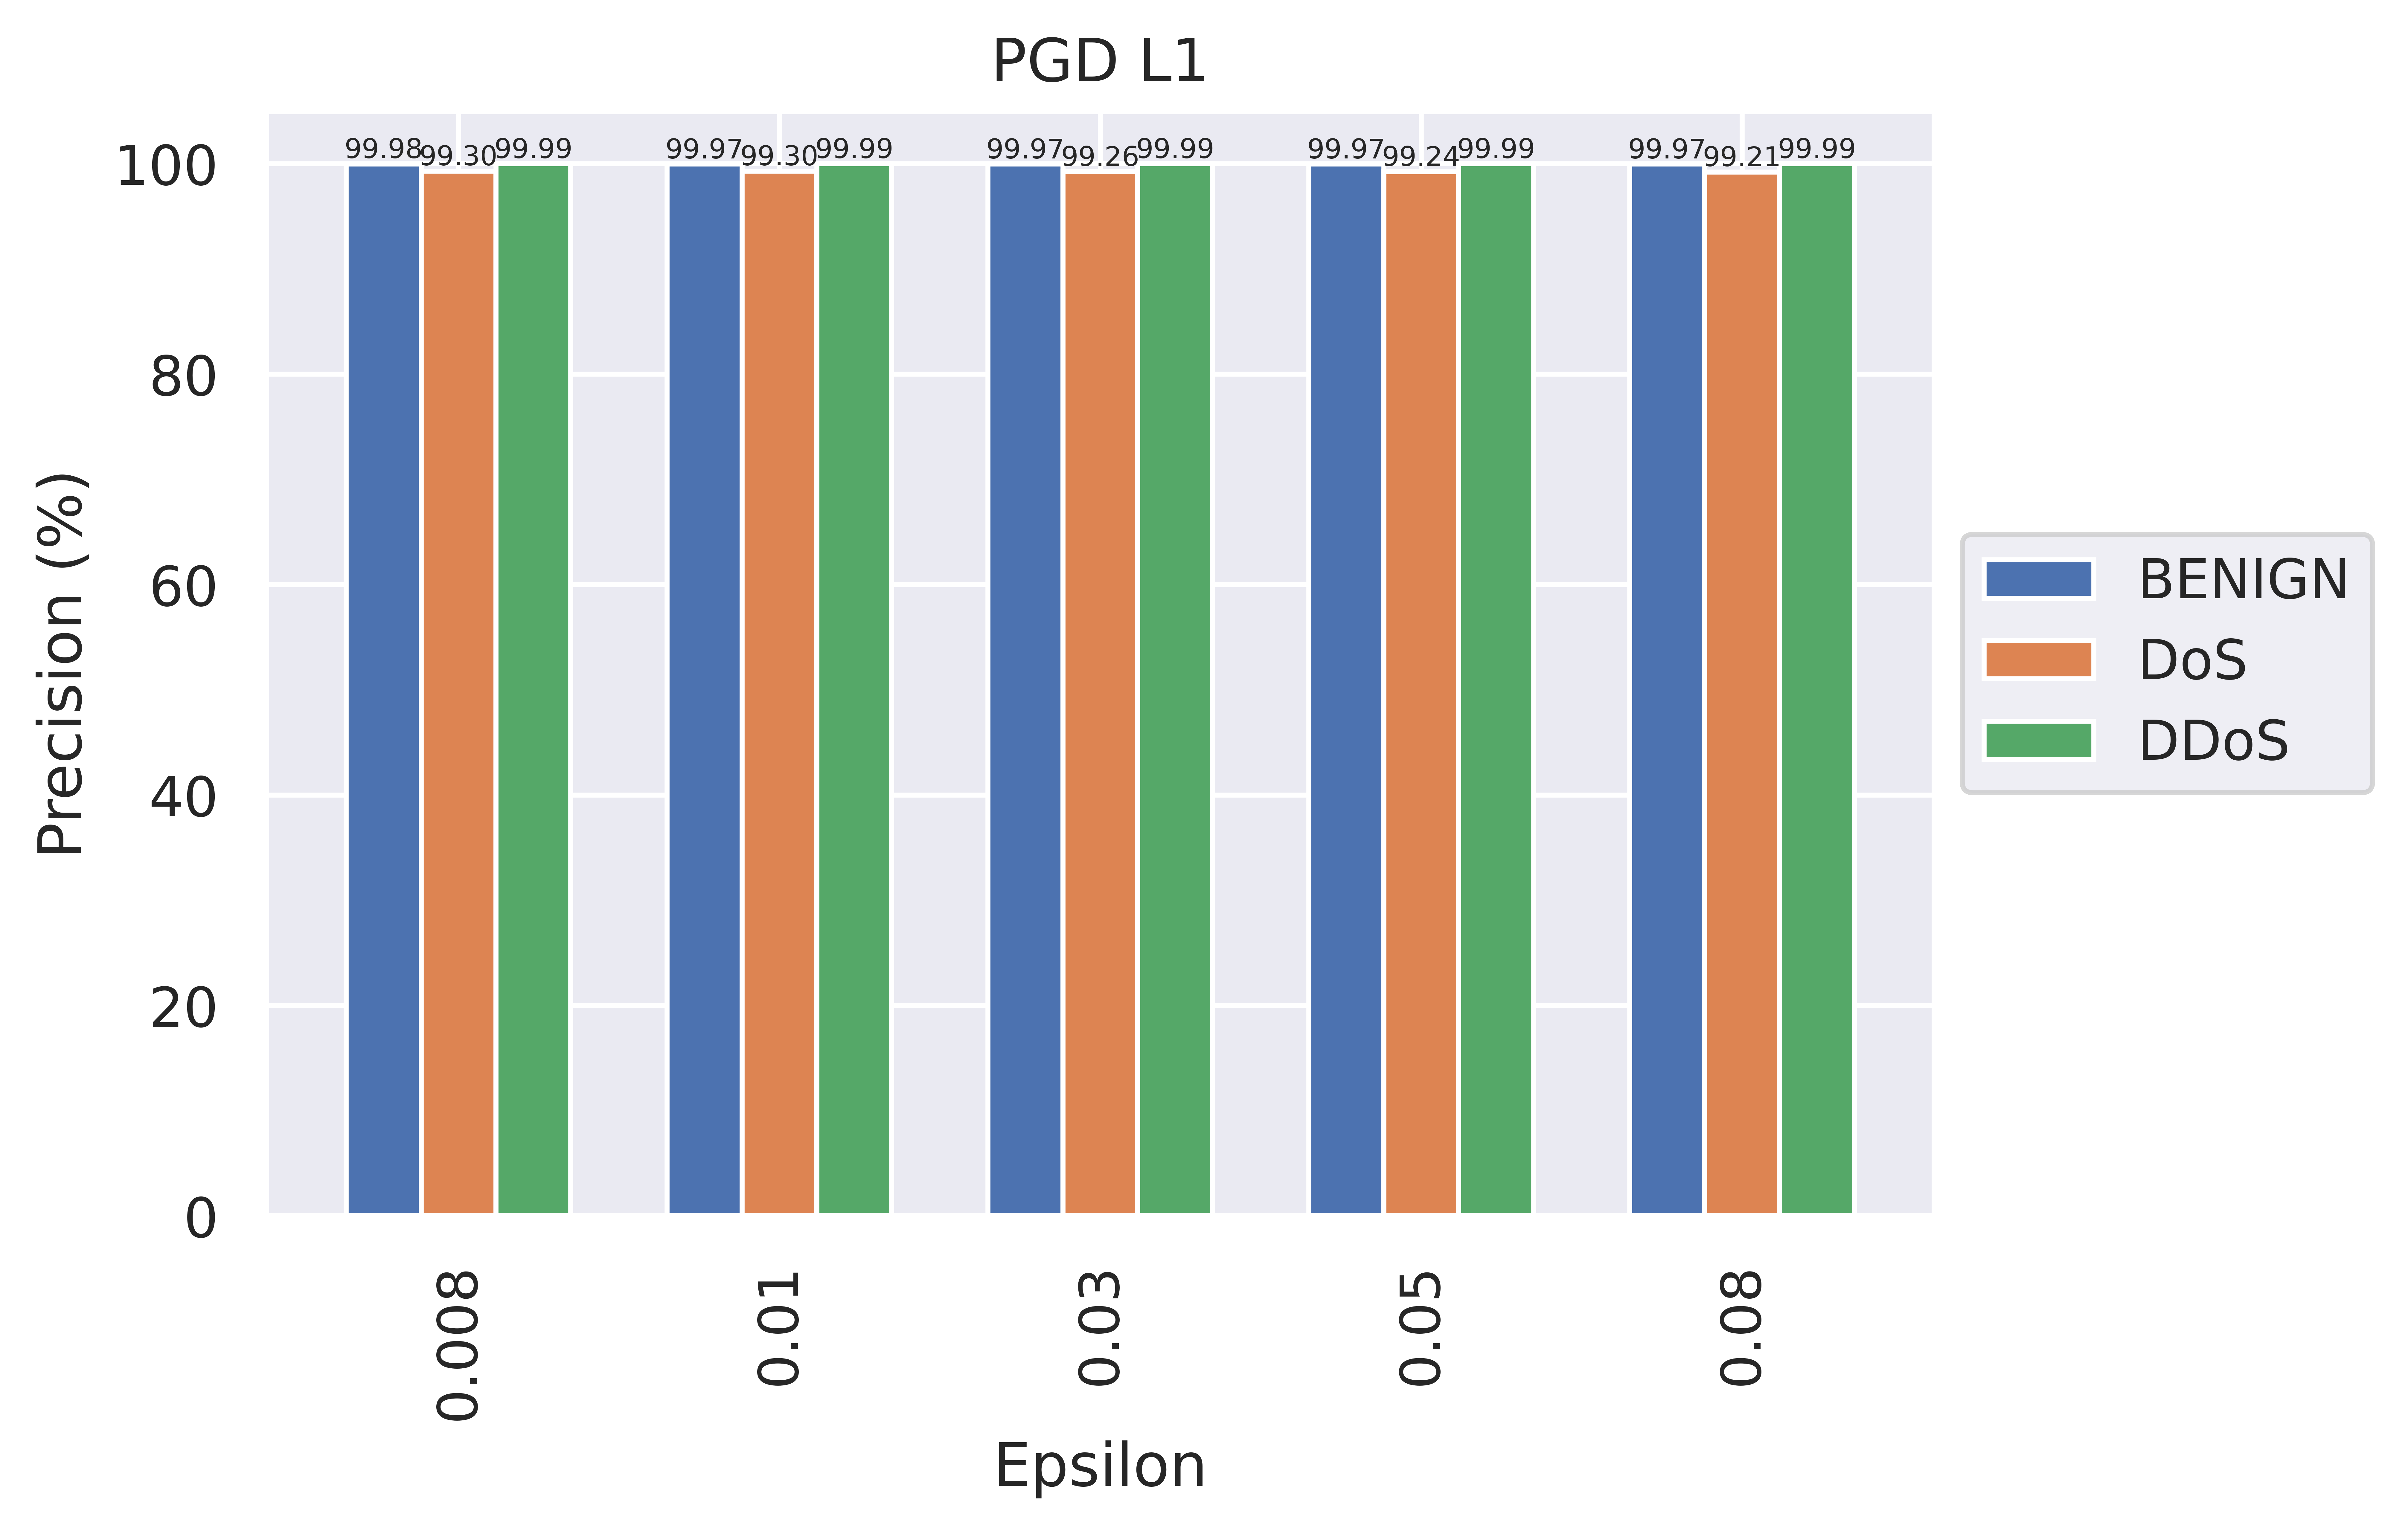
\includegraphics[width=\textwidth]{/home/wojtyla/Documentos/Artigo_2023/IJCNN_Suplementary/Figures//CIC_Clean_PGD L1_multi_paper.png}
			%caption{Figure}
			\label{fig:1}
		\end{subfigure}
		\hfill
		\begin{subfigure}[b]{0.45\textwidth}
			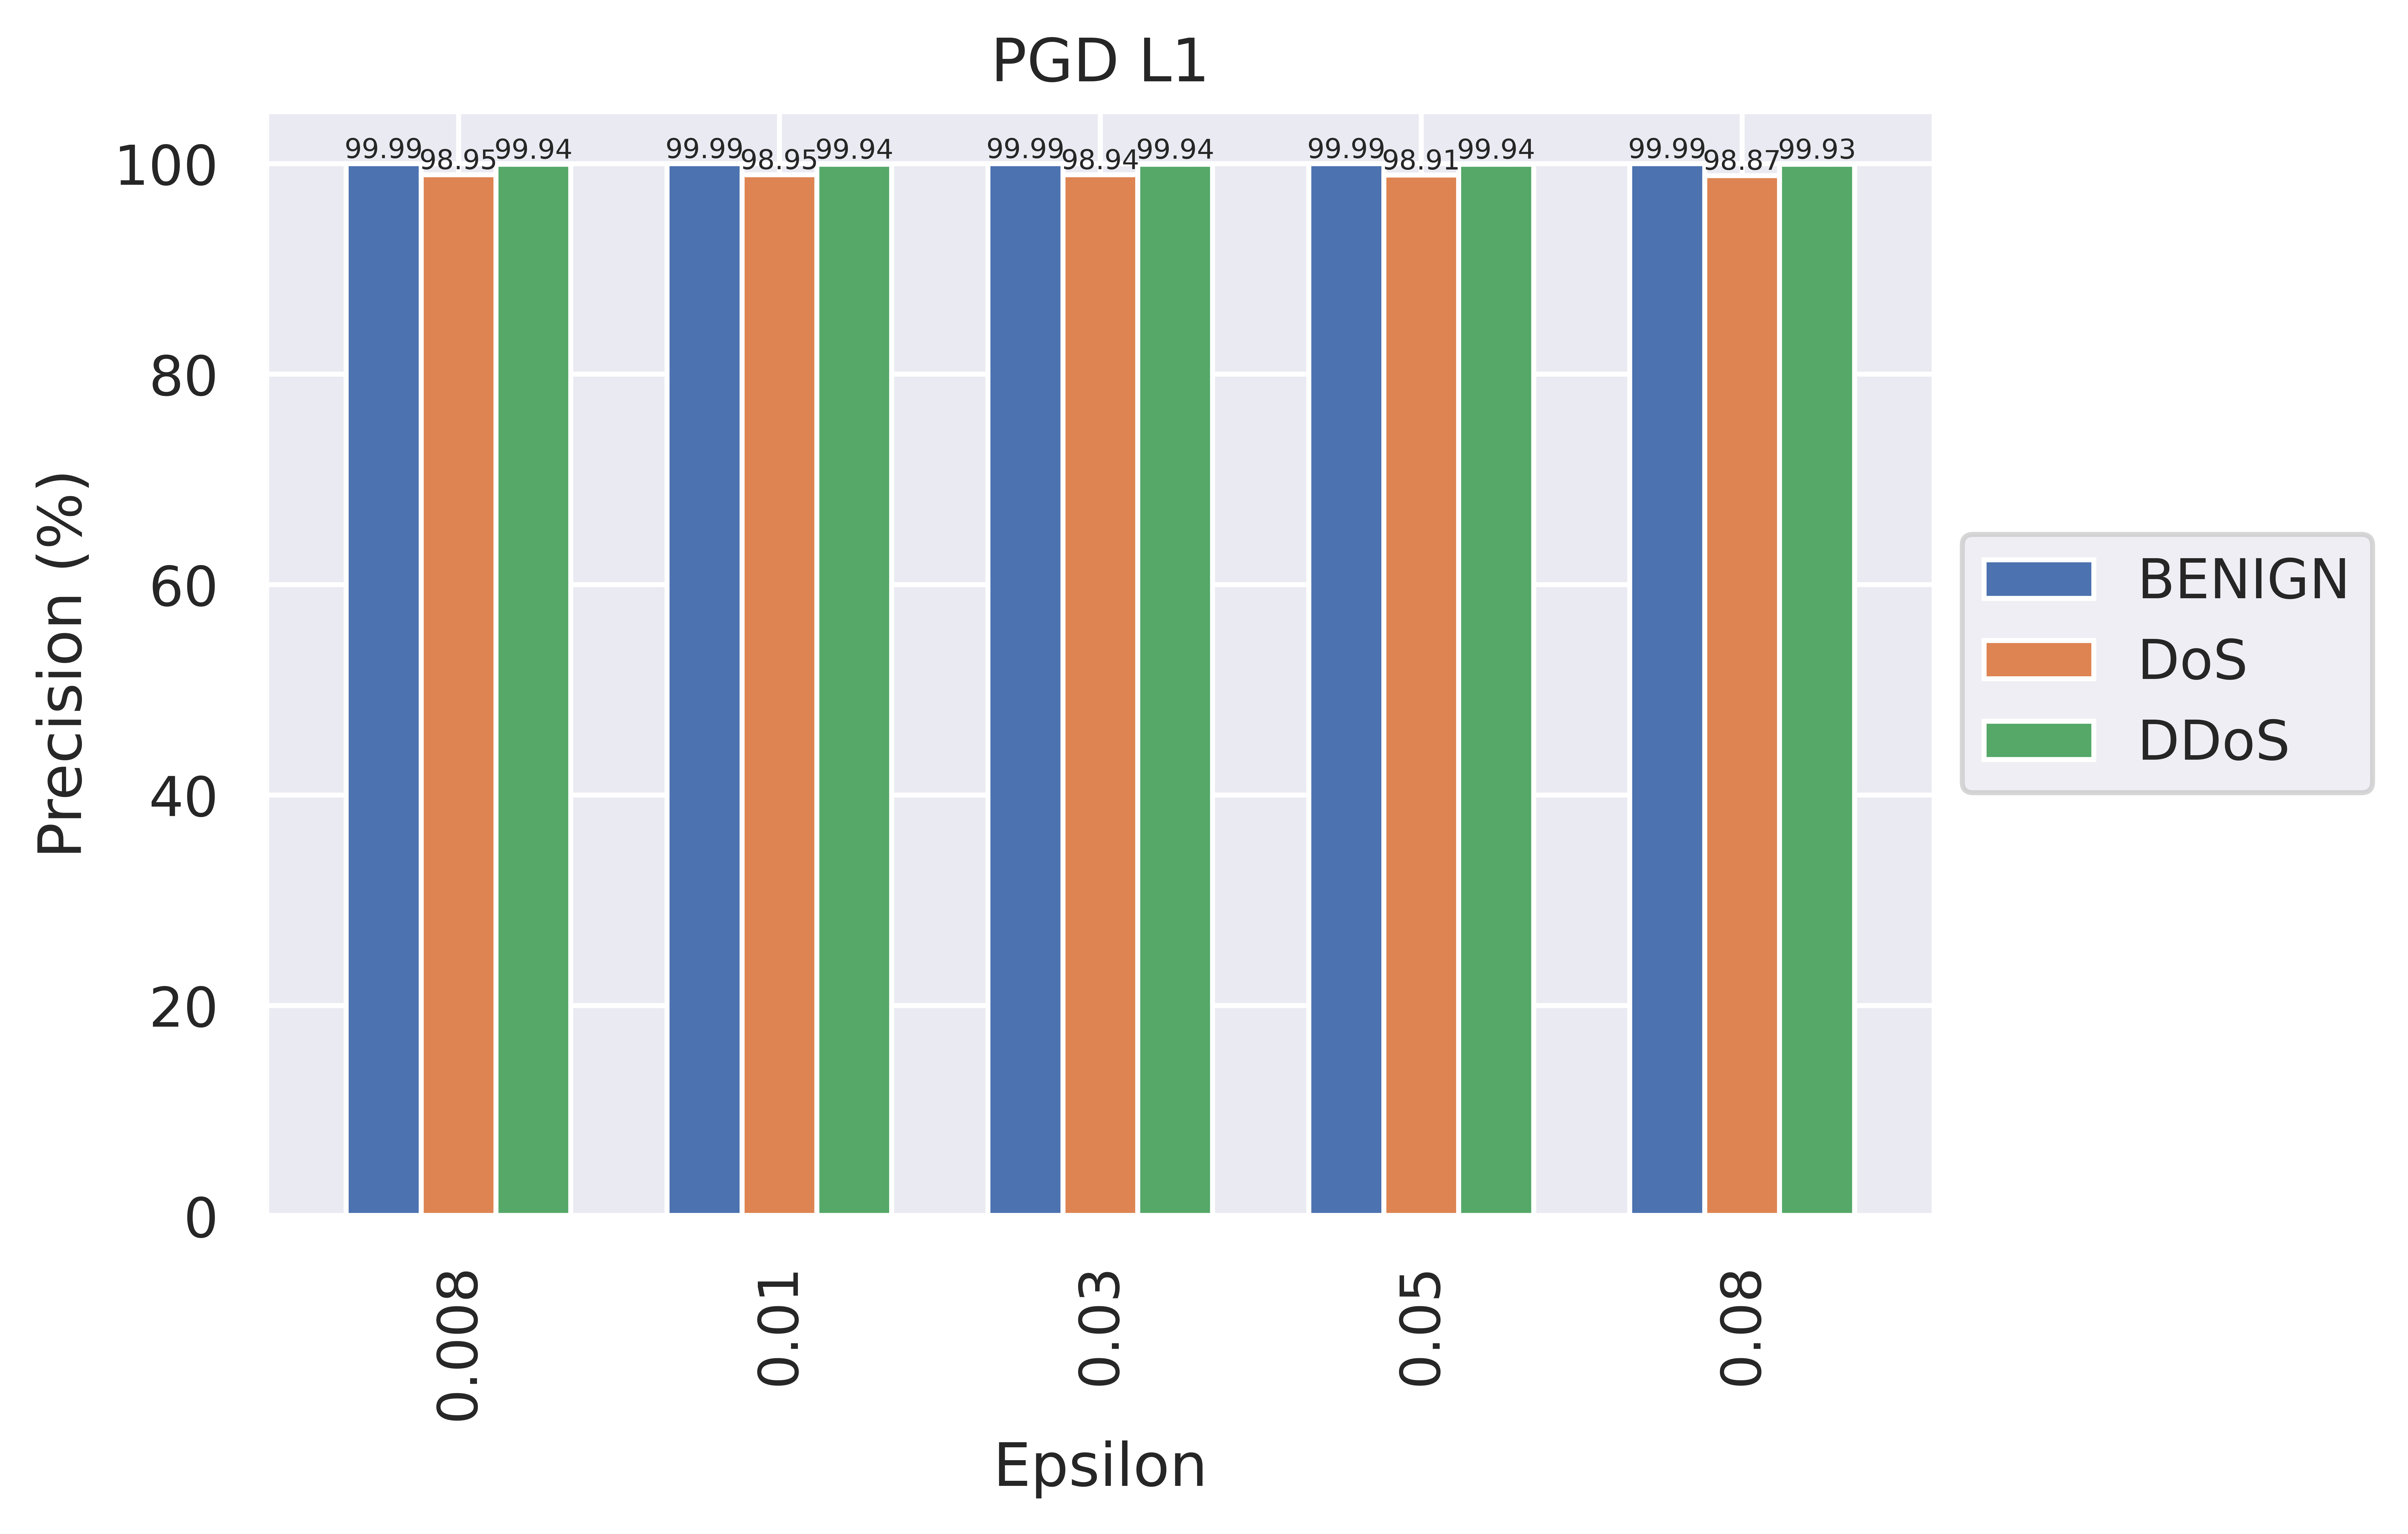
\includegraphics[width=\textwidth]{/home/wojtyla/Documentos/Artigo_2023/IJCNN_Suplementary/Figures///CIC_IDS_PGD L1_multi_paper.png}
			%caption{Figure}
			\label{fig:4}
		\end{subfigure}
		\vskip\baselineskip
		\begin{subfigure}[b]{0.45\textwidth}
			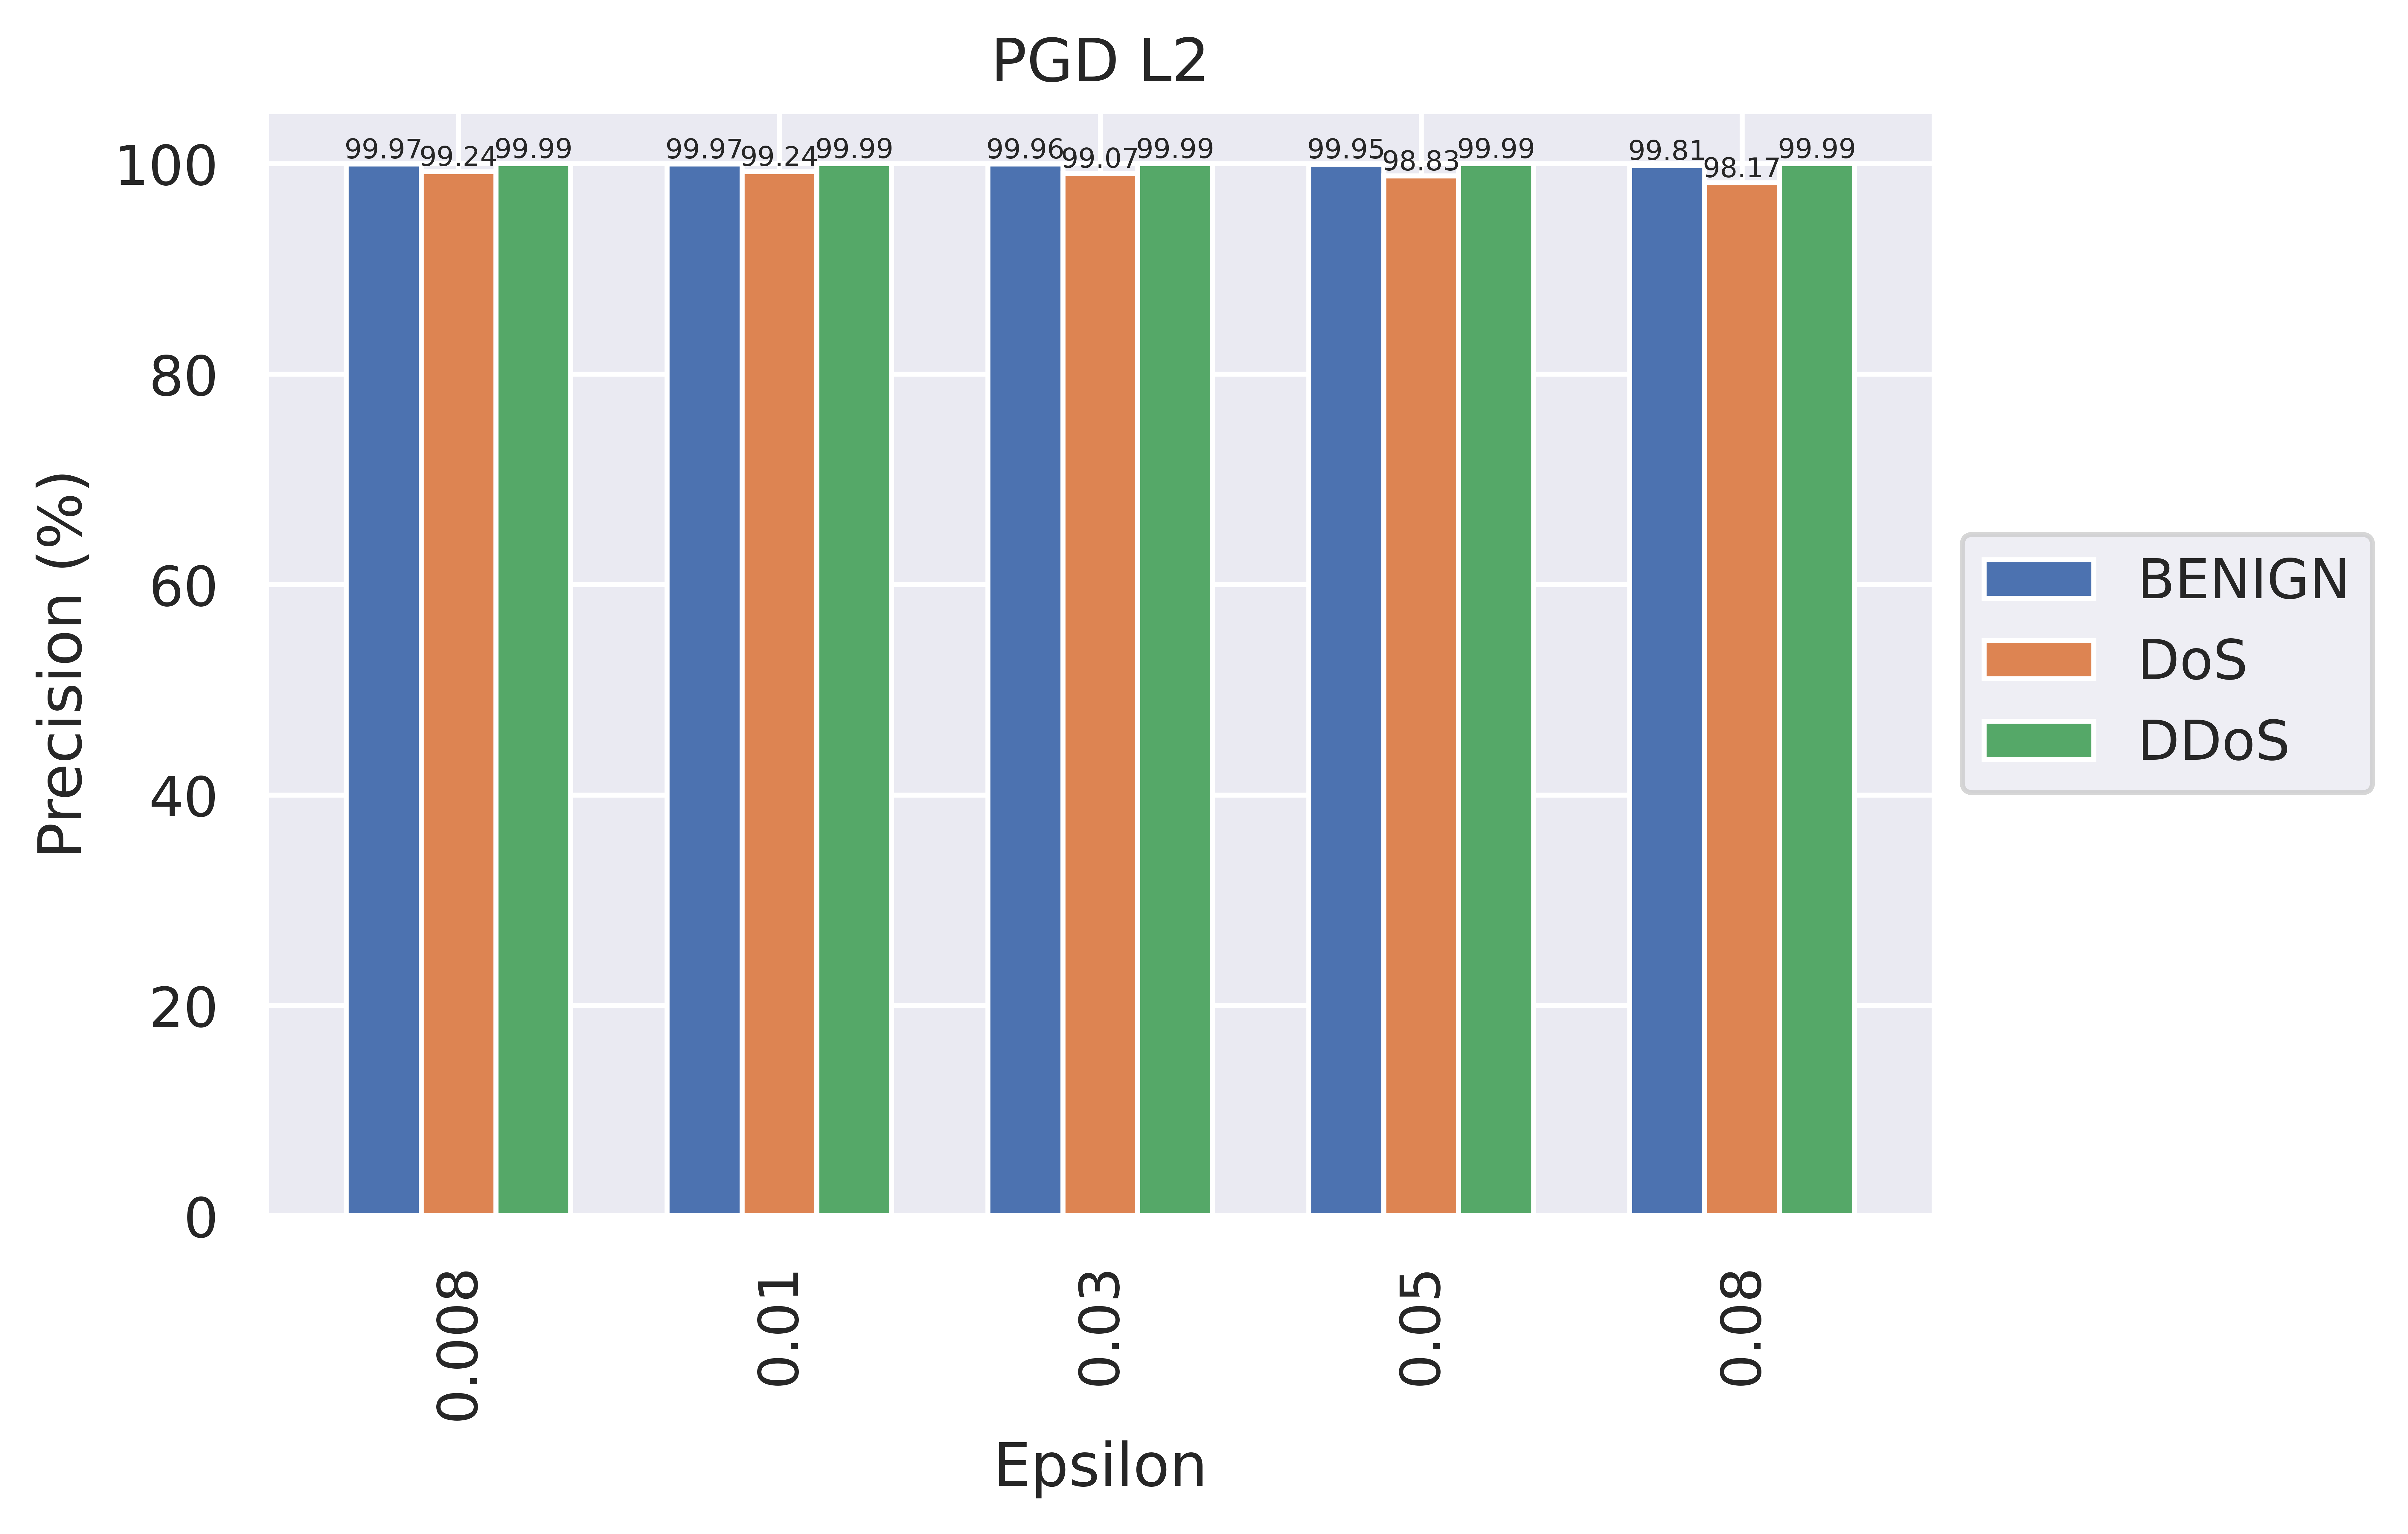
\includegraphics[width=\textwidth]{/home/wojtyla/Documentos/Artigo_2023/IJCNN_Suplementary/Figures//CIC_Clean_PGD L2_multi_paper.png}
			%caption{Figure}
			\label{fig:2}
		\end{subfigure}
		\hfill
		\begin{subfigure}[b]{0.45\textwidth}
			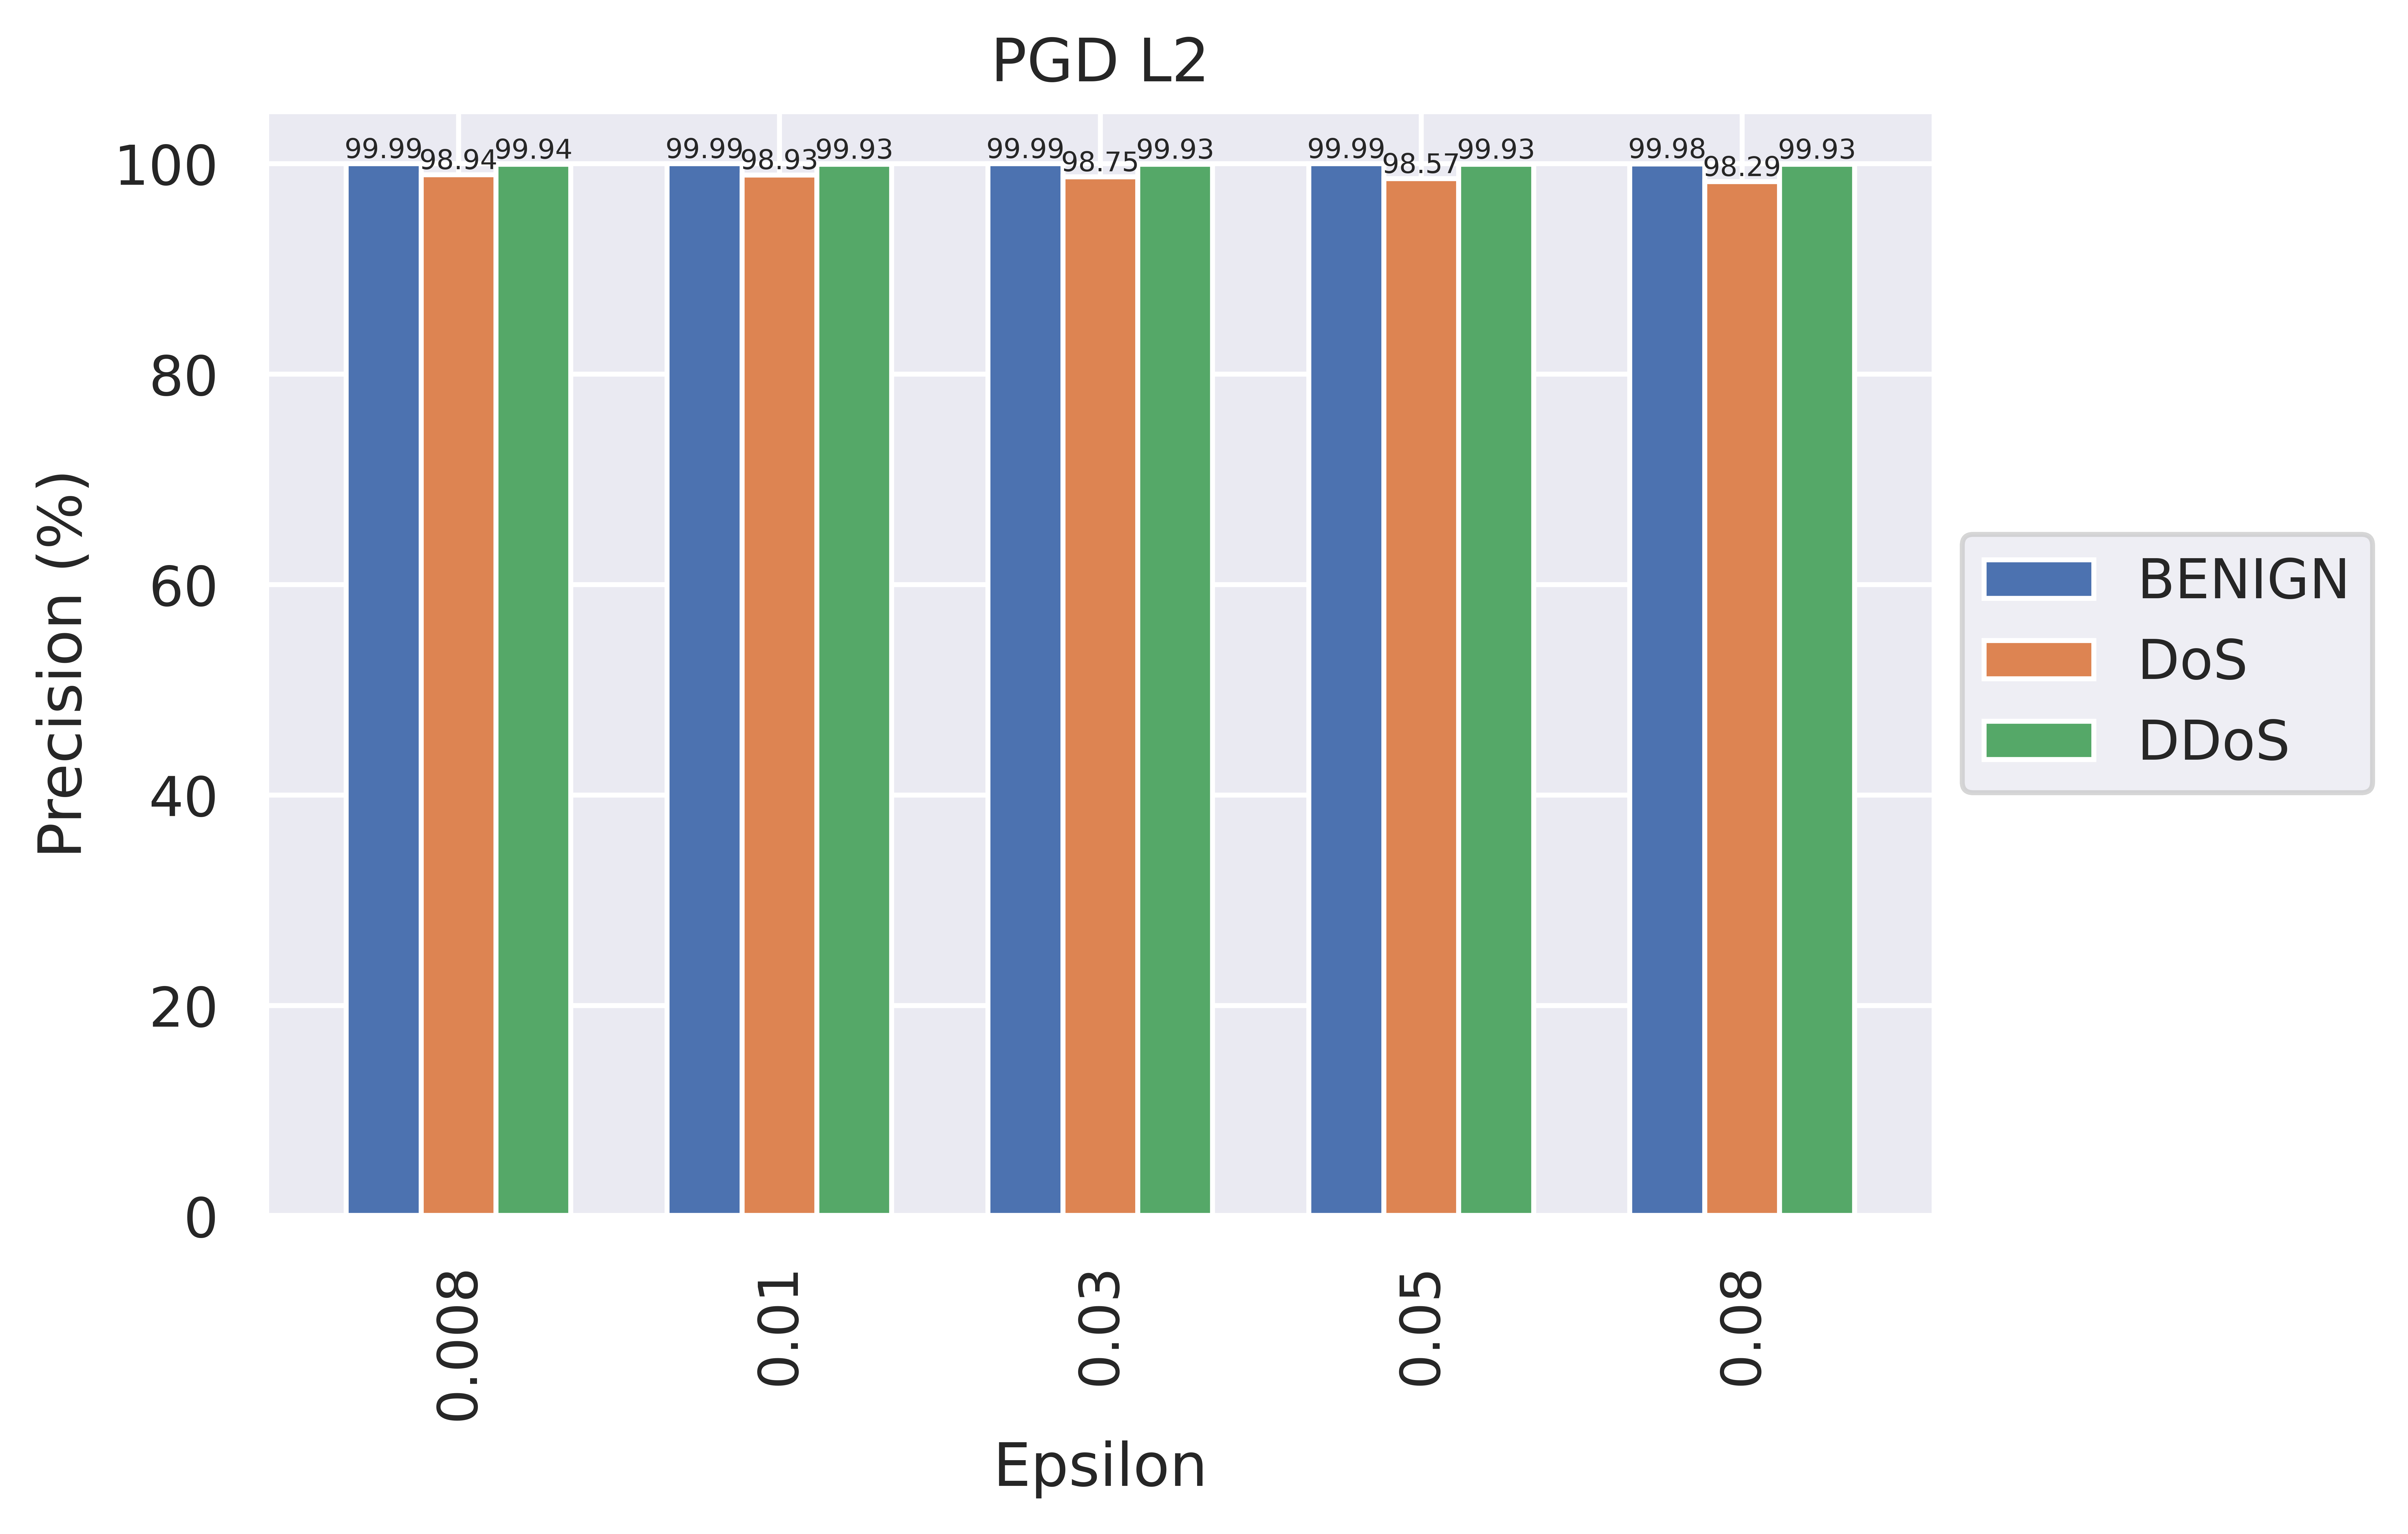
\includegraphics[width=\textwidth]{/home/wojtyla/Documentos/Artigo_2023/IJCNN_Suplementary/Figures//CIC_IDS_PGD L2_multi_paper.png}
			%caption{Figure}
			\label{fig:5}
		\end{subfigure}
		
		\vskip\baselineskip
		
		\begin{subfigure}[b]{0.45\textwidth}
			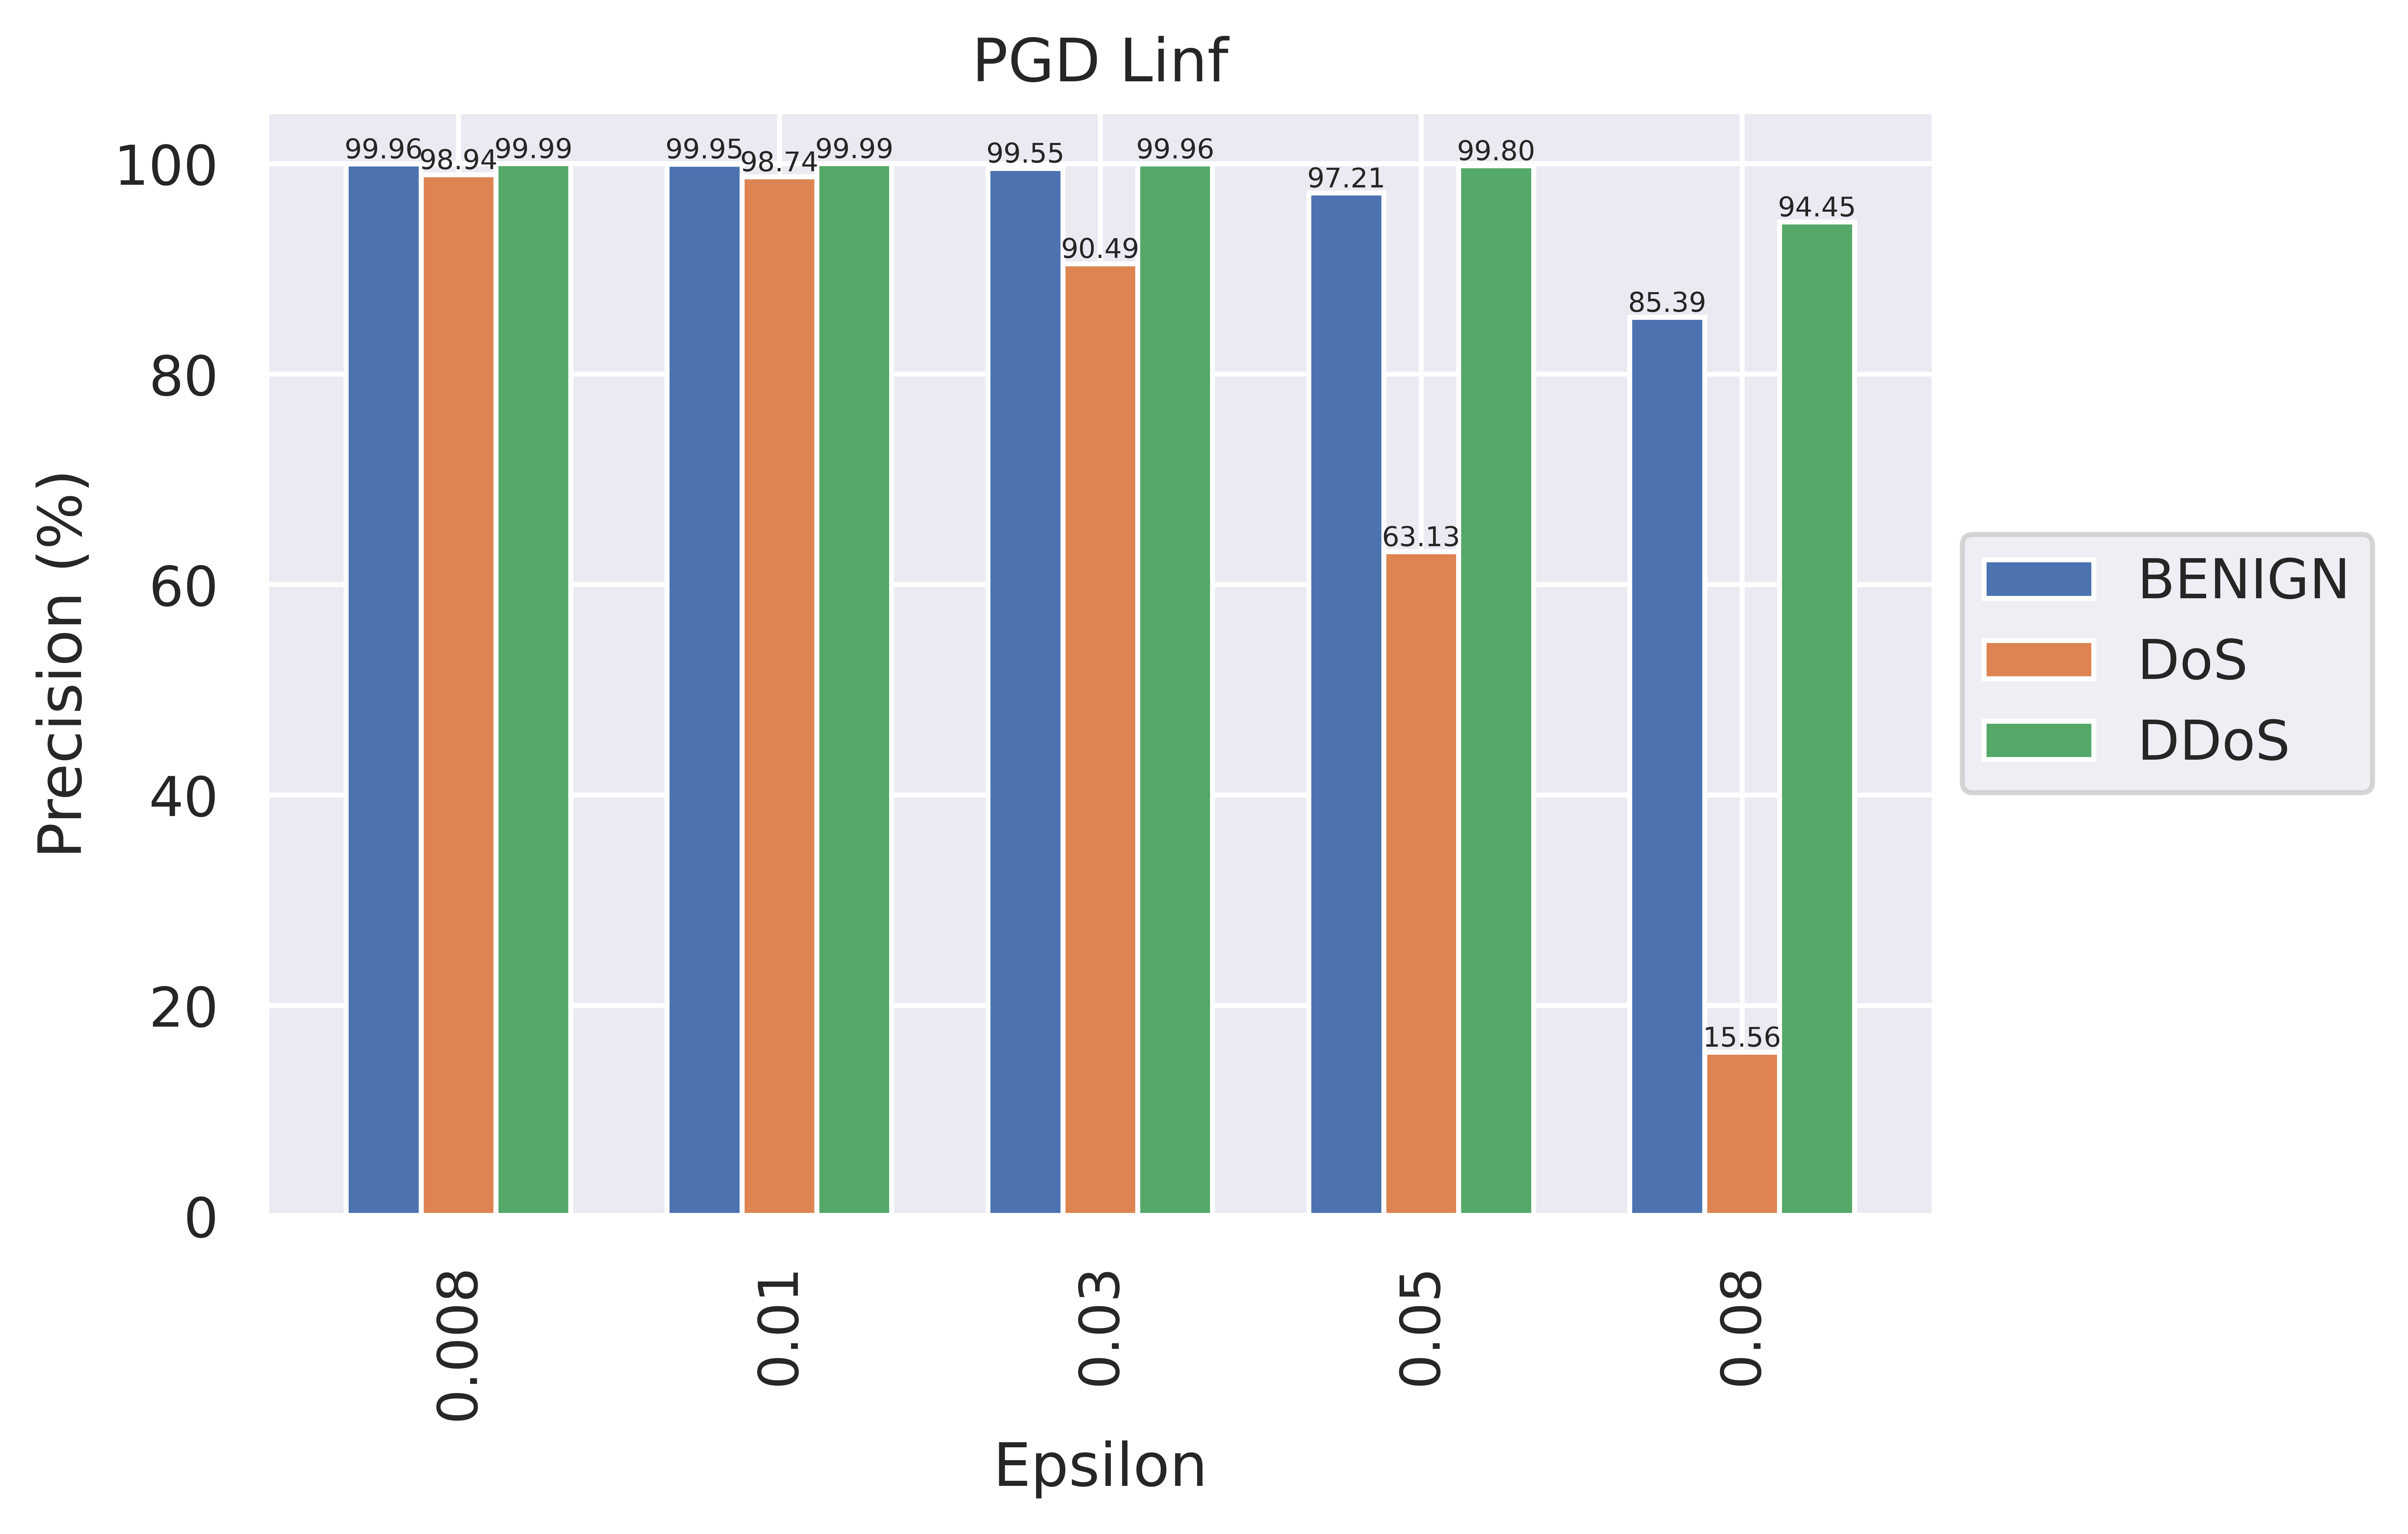
\includegraphics[width=\textwidth]{/home/wojtyla/Documentos/Artigo_2023/IJCNN_Suplementary/Figures//CIC_Clean_PGD Linf_multi_paper.png}
			%caption{Figure}
			\label{fig:3}
		\end{subfigure}			
		\hfill
		\begin{subfigure}[b]{0.45\textwidth}
			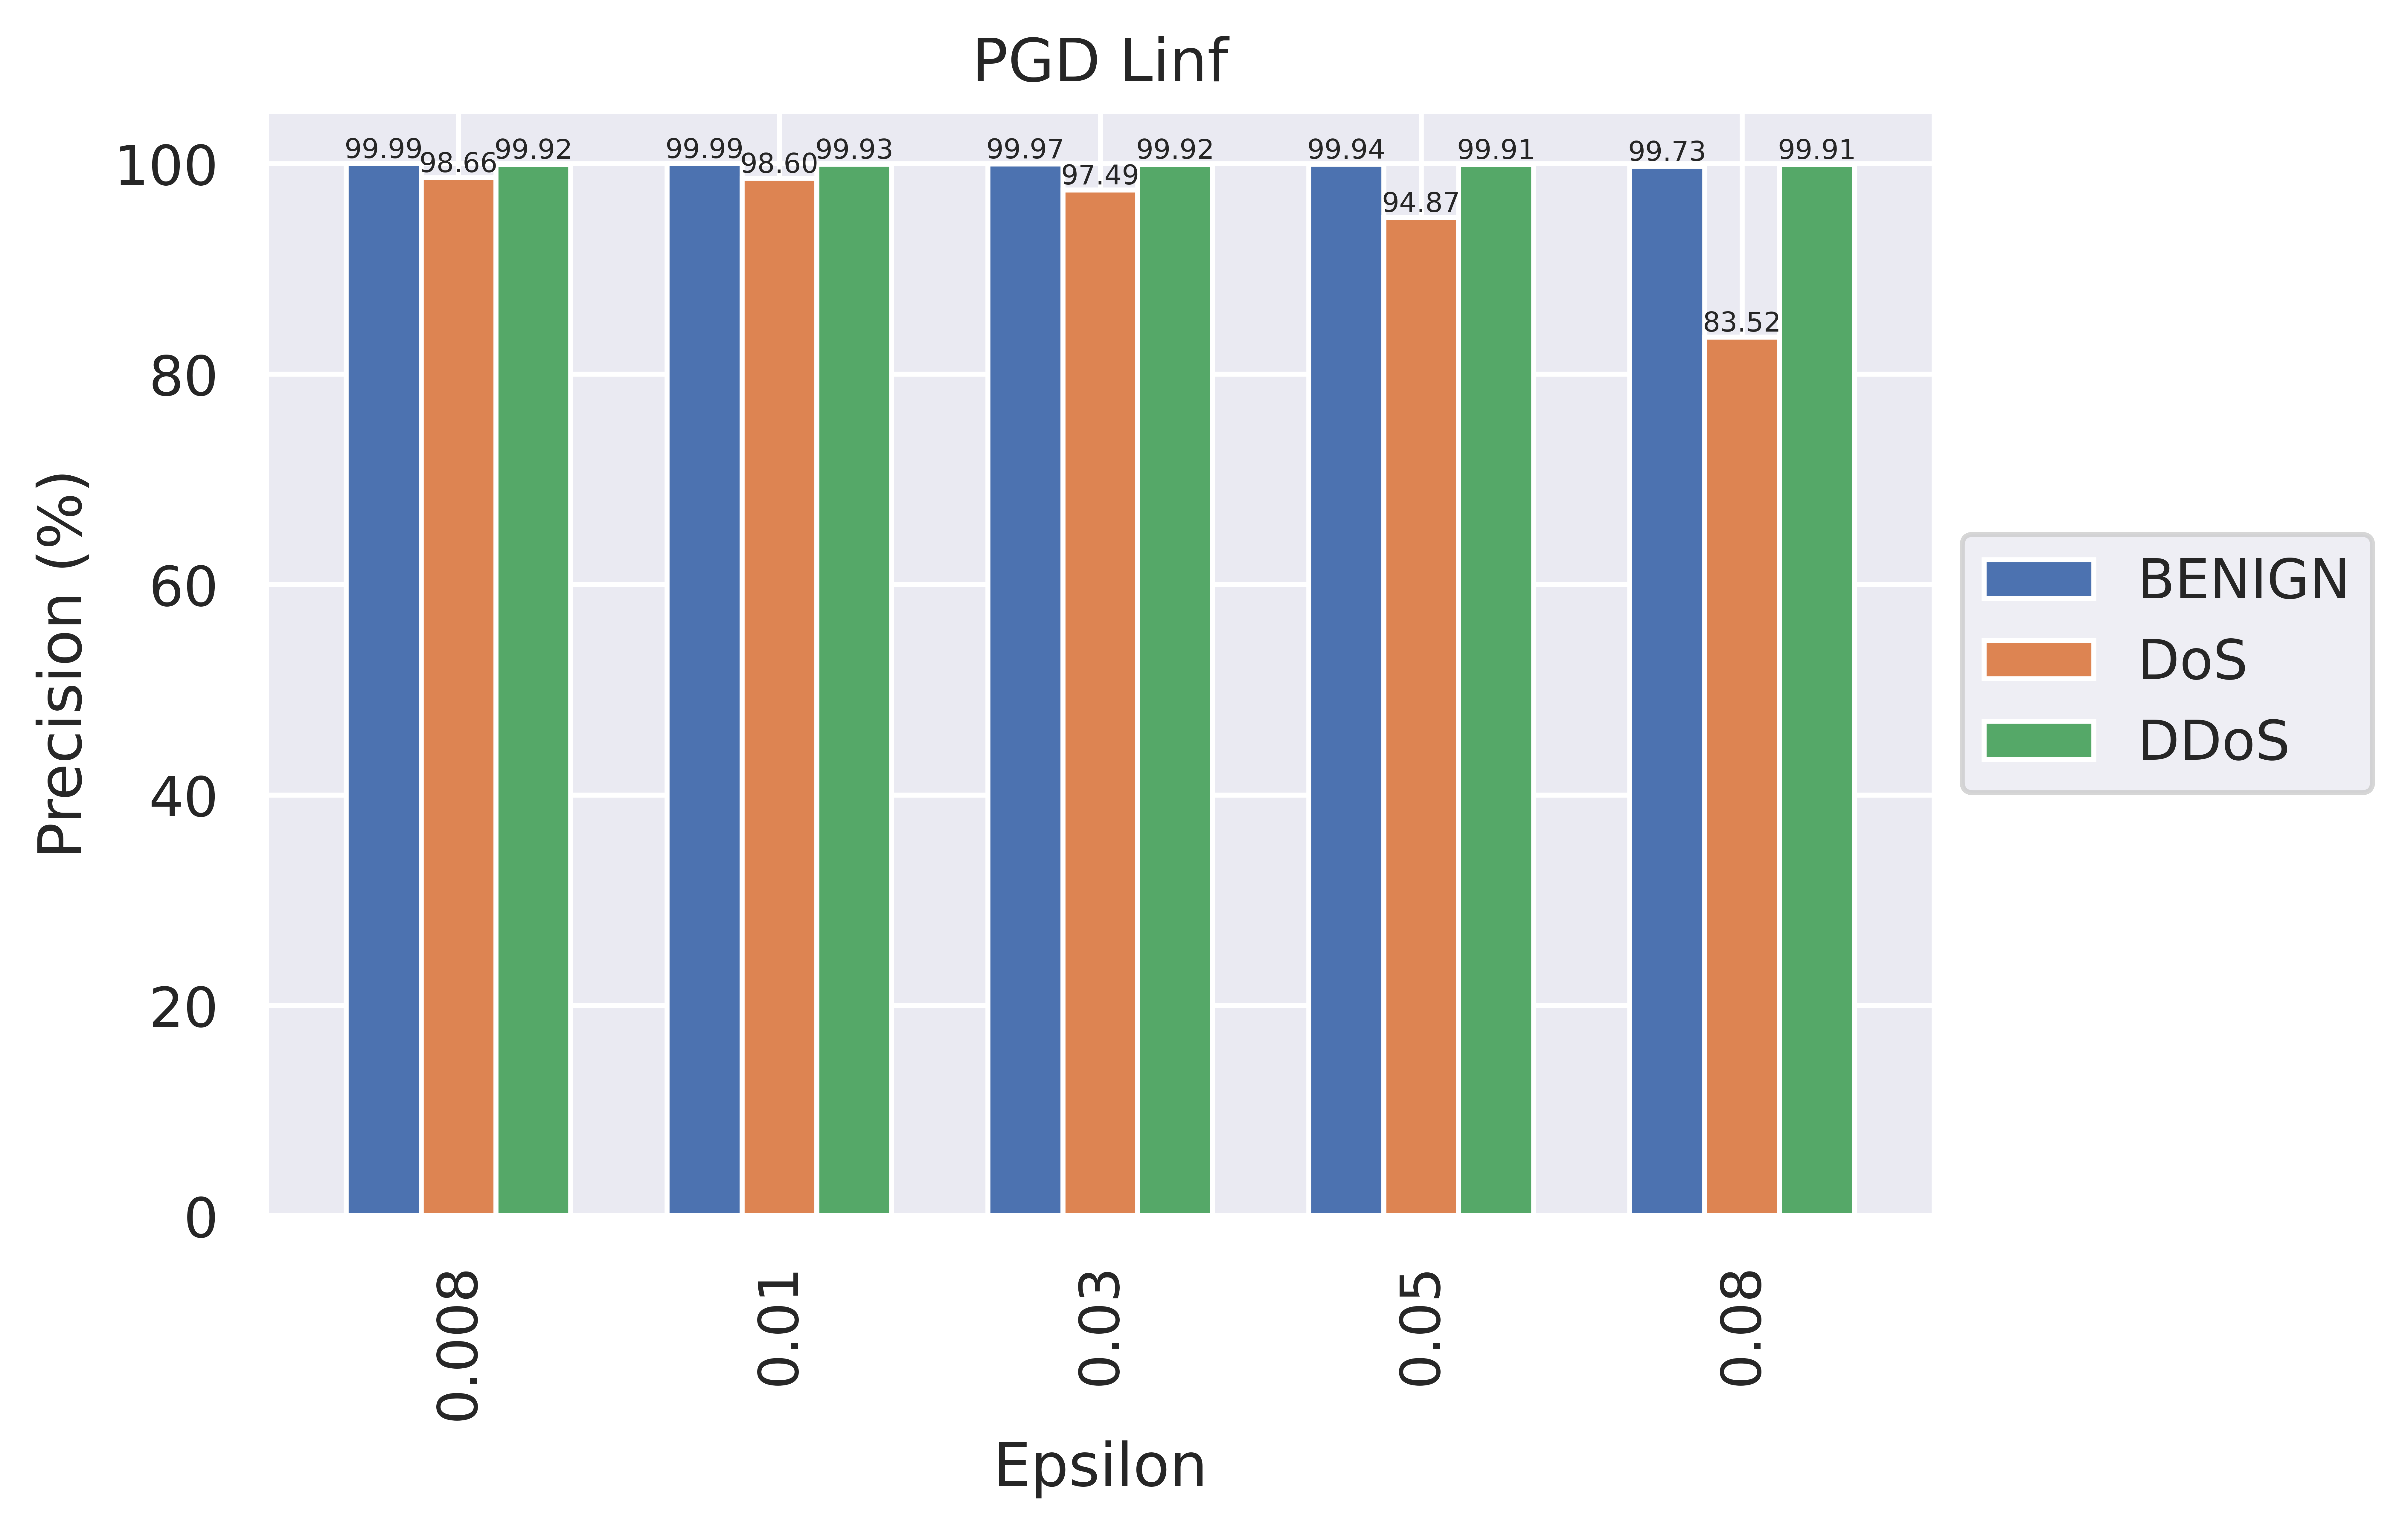
\includegraphics[width=\textwidth]{/home/wojtyla/Documentos/Artigo_2023/IJCNN_Suplementary/Figures//CIC_IDS_PGD Linf_multi_paper.png}
			%caption{Figure}
			\label{fig:6}
		\end{subfigure}
		\caption{Plots for PGD-100 attack on multiclass models with CIC IDS2017.Left:EnC model; Right:EnIDS model.}
		\label{fig:cic_pgd_multi}
	\end{figure}
	
	
	\subsection{UNSW-NB15}
	\FloatBarrier
	
	%\vspace*{-4cm}
	
	\begin{table}
		\caption{PGD-100 attack against EnC and EnIDS for binary classification on the UNSW-NB15 dataset.}
		\small
		\setlength{\tabcolsep}{3pt}
		\centering
		\label{tab:unsw_bin_pgd}

		\begin{tabular}{|c|c|c|c|c|c|c|c|c|c|c|c|c|}
			\hline
			\multirow{3}{*}{\textbf{Type}} & \multirow{3}{*}{\textbf{Norm}} & \multirow{3}{*}{\textbf{Metric}} & \multicolumn{10}{c|}{\textbf{\textsl{Epsilon} ($\epsilon$)}} \\
			\cline{4-13}
			& & & \multicolumn{2}{c|}{\textbf{0.008}} & \multicolumn{2}{c|}{\textbf{0.01}} & \multicolumn{2}{c|}{\textbf{0.03}} & \multicolumn{2}{c|}{\textbf{0.05}} & \multicolumn{2}{c|}{\textbf{0.08}} \\
			\cline{4-13}
			& & & \textbf{\textsl{Benign}} & \textbf{\textsl{Attacks}} & \textbf{\textsl{Benign}} & \textbf{\textsl{Attacks}} & \textbf{\textsl{Benign}} & \textbf{\textsl{Attacks}} & \textbf{\textsl{Benign}} & \textbf{\textsl{Attacks}} & \textbf{\textsl{Benign}} & \textbf{\textsl{Attacks}} \\
			\hline
			\multirow{9}{*}{EnC} 
			& \multirow{3}{*}{\( \ell_1 \)} & Precision & 100.00 & 85.99 & 100.00 & 85.99 & 100.00 & 85.94 & 100.00 & 85.92 & 100.00 & 85.90
			\\
			
			&  & Recall & 99.66 & 100.00 & 99.66 & 100.00 & 99.66 & 100.00 & 99.66 & 100.00 & 99.66 & 99.98
			\\
			
			&  & ROC-AUC & 99.98 & 99.98 & 99.98 & 99.98 & 99.98 & 99.98 & 99.98 & 99.98 & 99.97 & 99.97
			\\
			\cline{2-13}
			& \multirow{3}{*}{\( \ell_2 \)} & Precision & 100.00 & 85.94 & 100.00 & 85.92 & 100.00 & 85.90 & 100.00 & 85.85 & 99.99 & 85.77
			\\
			
			&  & Recall & 99.66 & 100.00 & 99.66 & 100.00 & 99.66 & 99.98 & 99.66 & 99.98 & 99.65 & 99.71
			\\
			
			&  & ROC-AUC & 99.98 & 99.98 & 99.98 & 99.98 & 99.97 & 99.97 & 99.95 & 99.95 & 99.93 & 99.93
			\\
			\cline{2-13}
			& \multirow{3}{*}{\( \ell_\infty \)} & Precision & 100.00 & 85.90 & 100.00 & 85.89 & 99.98 & 85.66 & 99.93 & 84.82 & 99.73 & 78.78
			\\
			
			&  & Recall & 99.66 & 99.98 & 99.66 & 99.98 & 99.65 & 99.05 & 99.64 & 96.49 & 99.51 & 87.24
			\\
			
			&  & ROC-AUC & 99.97 & 99.97 & 99.96 & 99.96 & 99.90 & 99.90 & 99.76 & 99.76 & 99.49 & 99.59
			\\
			\hline
			\multirow{9}{*}{EnIDS} & \multirow{3}{*}{\( \ell_1 \)} & Precision & 99.94 & 60.59 & 99.94 & 60.47 & 99.93 & 59.71 & 99.92 & 59.45 & 99.91 & 59.24
			\\
			
			&  & Recall & 98.68 & 97.12 & 98.68 & 97.10 & 98.64 & 96.53 & 98.63 & 96.35 & 98.62 & 95.97
			\\
			
			&  & ROC-AUC & 99.87 & 99.87 & 99.87 & 99.87 & 99.85 & 99.84 & 99.83 & 99.83 & 99.79 & 99.79
			\\
			\cline{2-13}
			& \multirow{3}{*}{\( \ell_2 \)} & Precision & 99.94 & 60.34 & 99.93 & 60.27 & 99.92 & 59.23 & 99.91 & 59.12 & 99.92 & 58.91
			\\
			
			&  & Recall & 98.67 & 96.96 & 98.67 & 96.89 & 98.62 & 96.02 & 98.62 & 95.79 & 98.60 & 96.02
			\\
			
			&  & ROC-AUC & 99.86 & 99.86 & 99.85 & 99.85 & 99.82 & 99.82 & 99.78 & 99.78 & 99.73 & 99.73
			\\
			\cline{2-13}
			& \multirow{3}{*}{\( \ell_\infty \)} & Precision & 99.92 & 56.82 & 99.92 & 56.97 & 99.91 & 58.58 & 99.90 & 47.59 & 99.88 & 51.82
			\\
			
			&  & Recall & 98.47 & 96.24 & 98.49 & 96.04 & 98.59 & 95.66 & 97.81 & 95.41 & 98.17 & \cellcolor{yellow!50}\textbf{94.42}
			\\
			
			&  & ROC-AUC & 99.79 & 99.79 & 99.72 & 99.72 & 99.67 & 99.66 & 99.59 & 99.59 & 99.58 & 99.58
			\\
			\hline
		\end{tabular}

	\end{table}

	
	
	\begin{figure}[H]
		\centering
		\begin{subfigure}[b]{0.45\textwidth}
			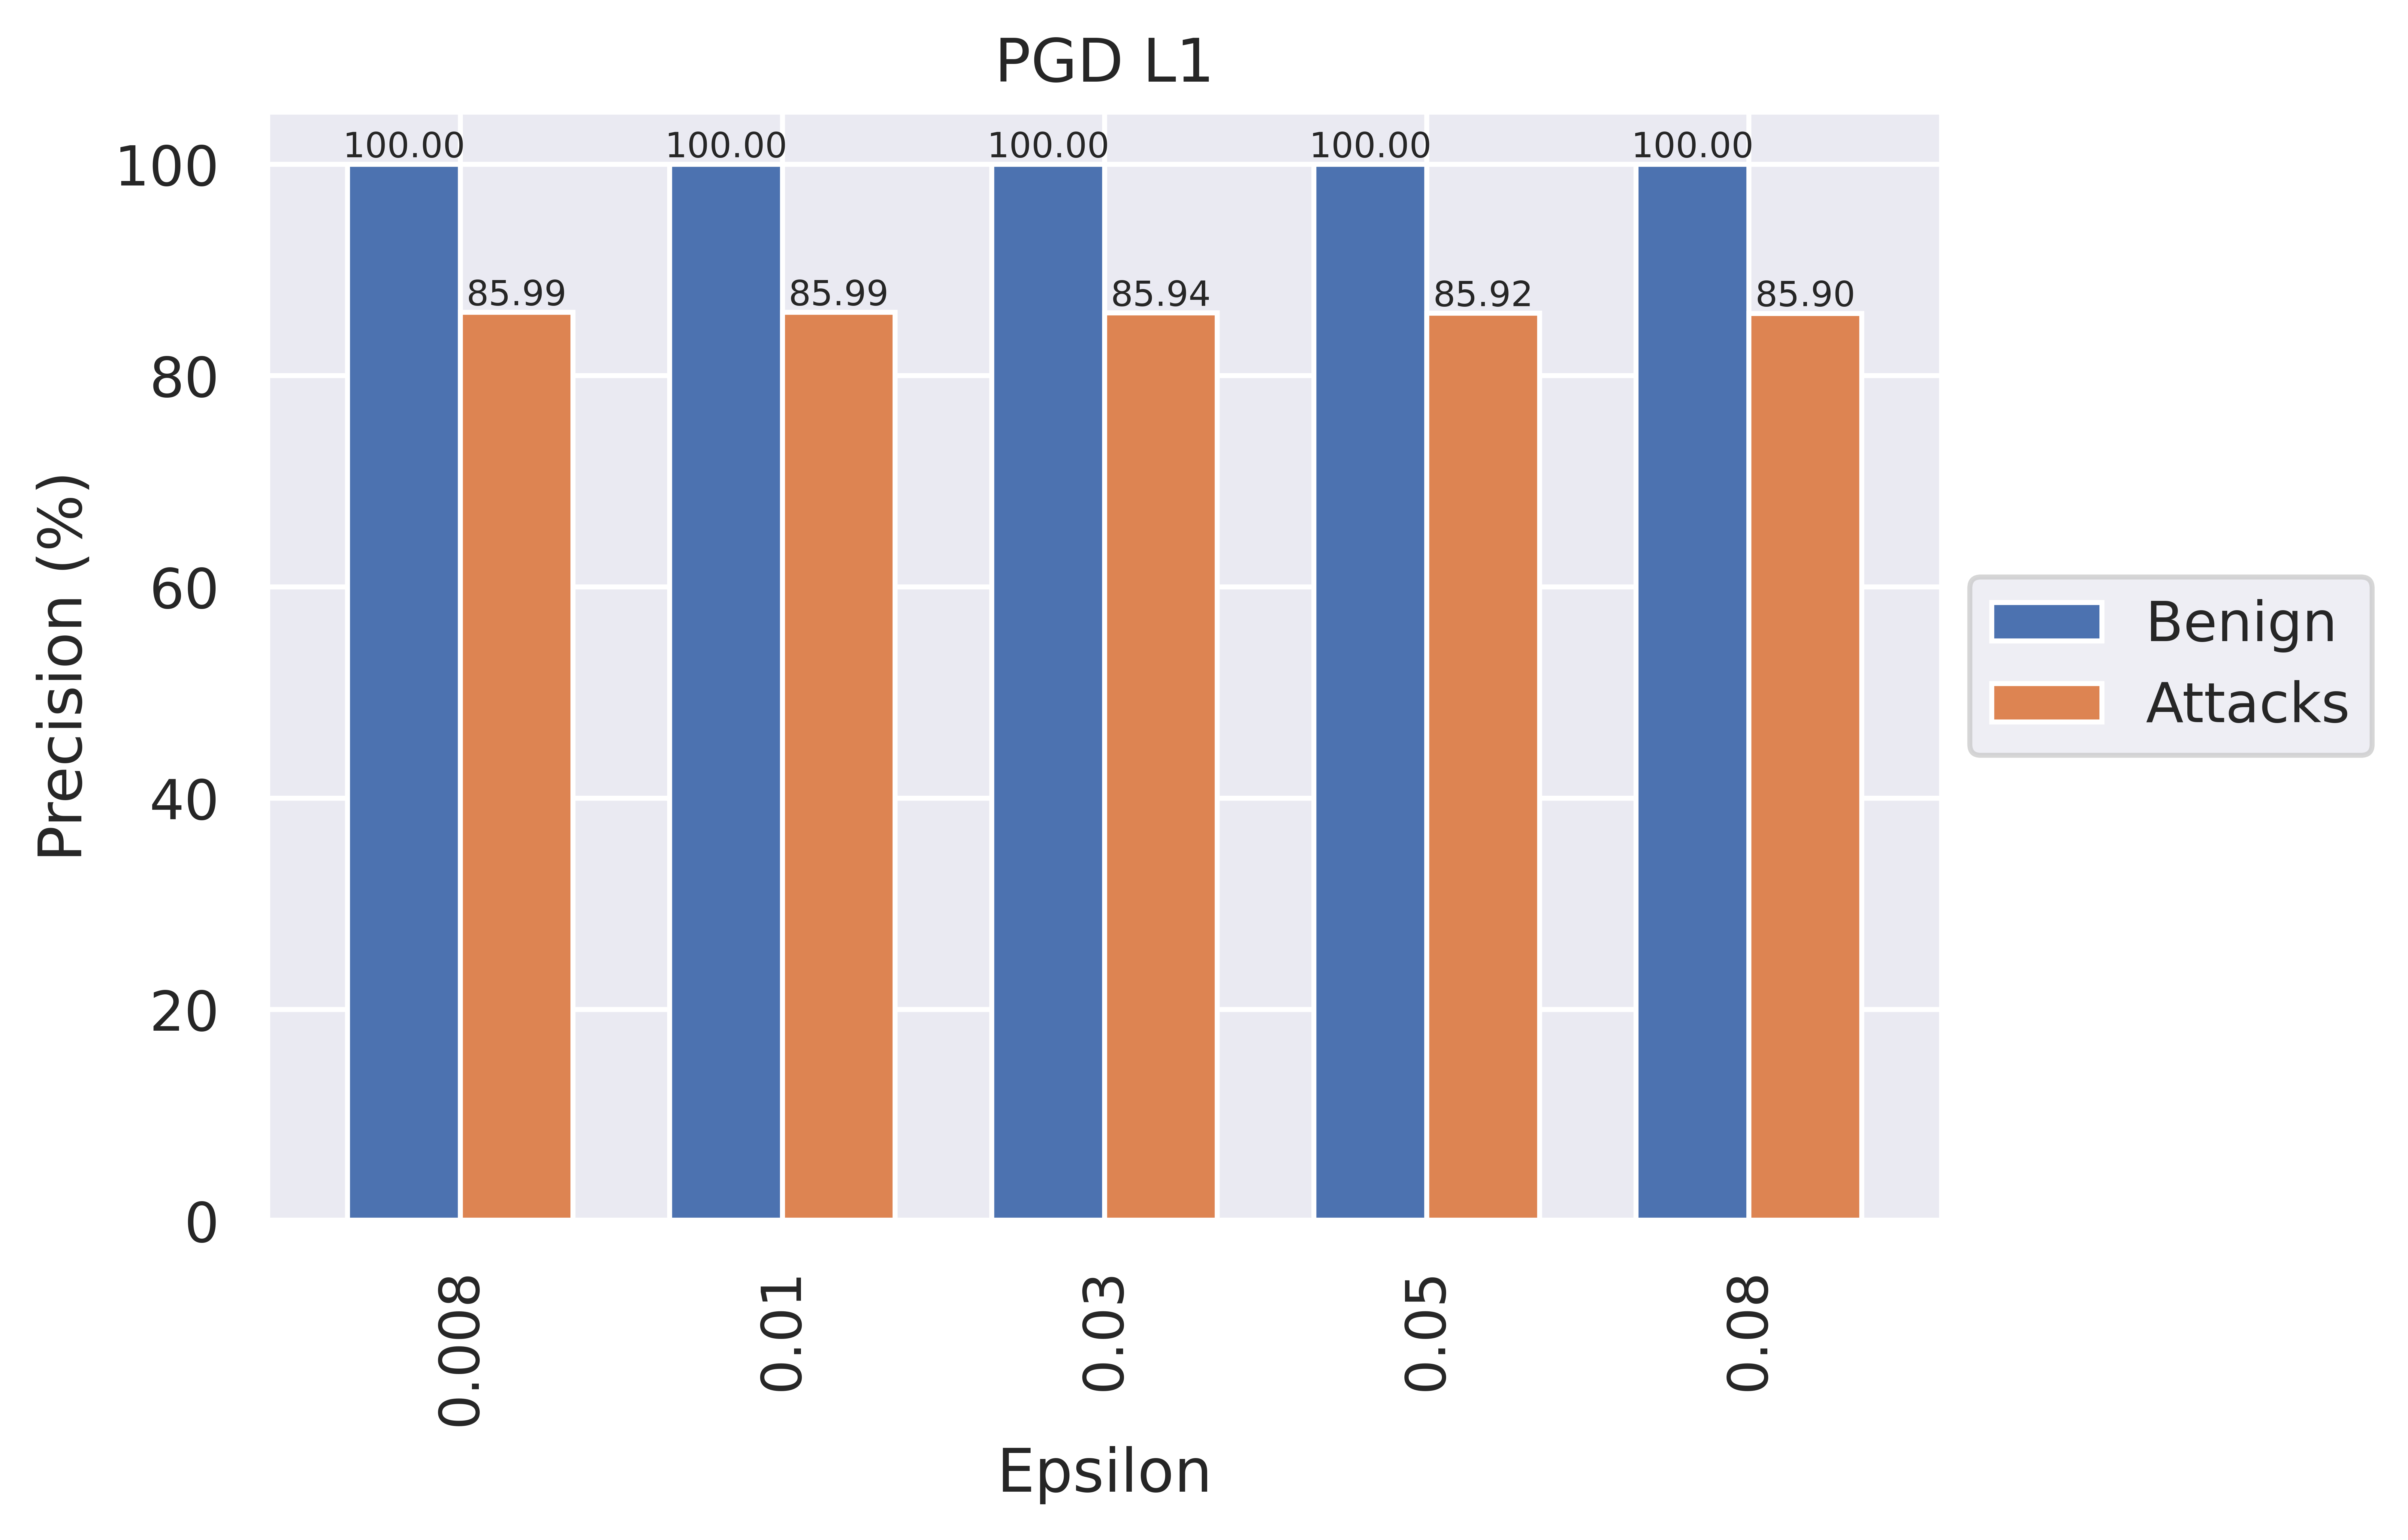
\includegraphics[width=\textwidth]{/home/wojtyla/Documentos/Artigo_2023/IJCNN_Suplementary/Figures//UNSW_Clean_PGD L1_bin_paper.png}
			%caption{Figure}
			\label{fig:1}
		\end{subfigure}
		\hfill
		\begin{subfigure}[b]{0.45\textwidth}
			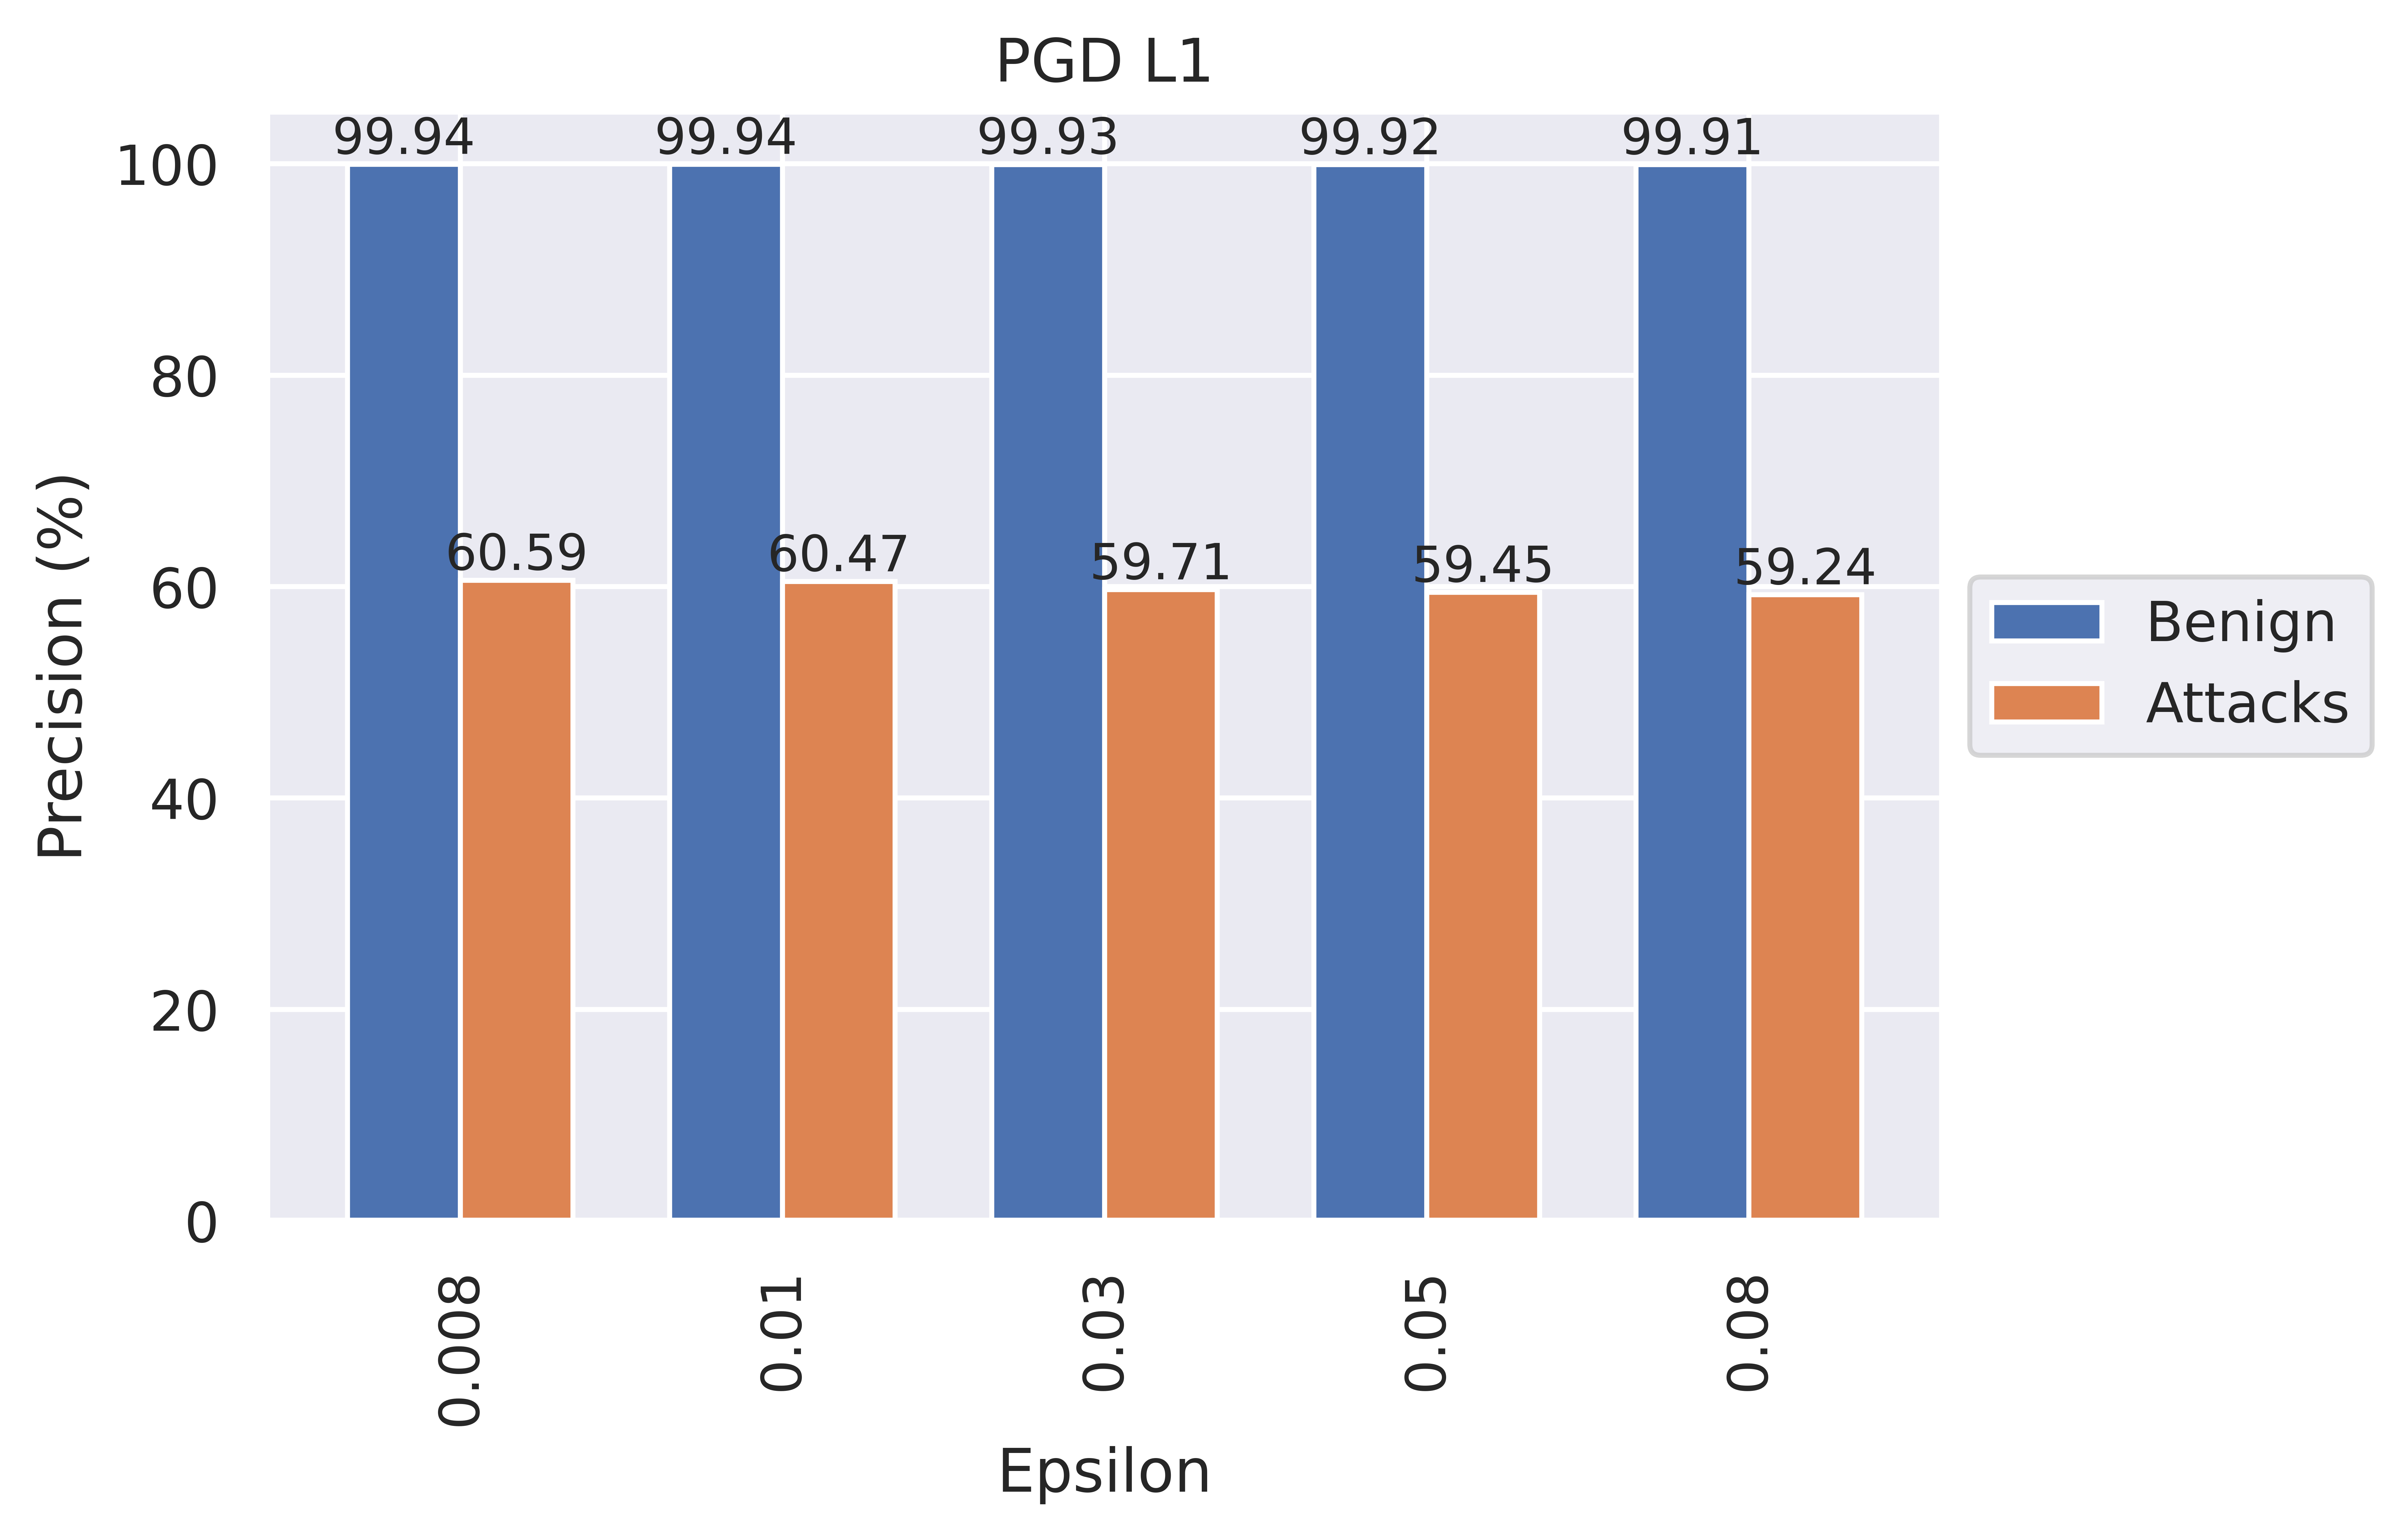
\includegraphics[width=\textwidth]{/home/wojtyla/Documentos/Artigo_2023/IJCNN_Suplementary/Figures///UNSW_IDS_PGD L1_bin_paper.png}
			%caption{Figure}
			\label{fig:4}
		\end{subfigure}
		\vskip\baselineskip
		\begin{subfigure}[b]{0.45\textwidth}
			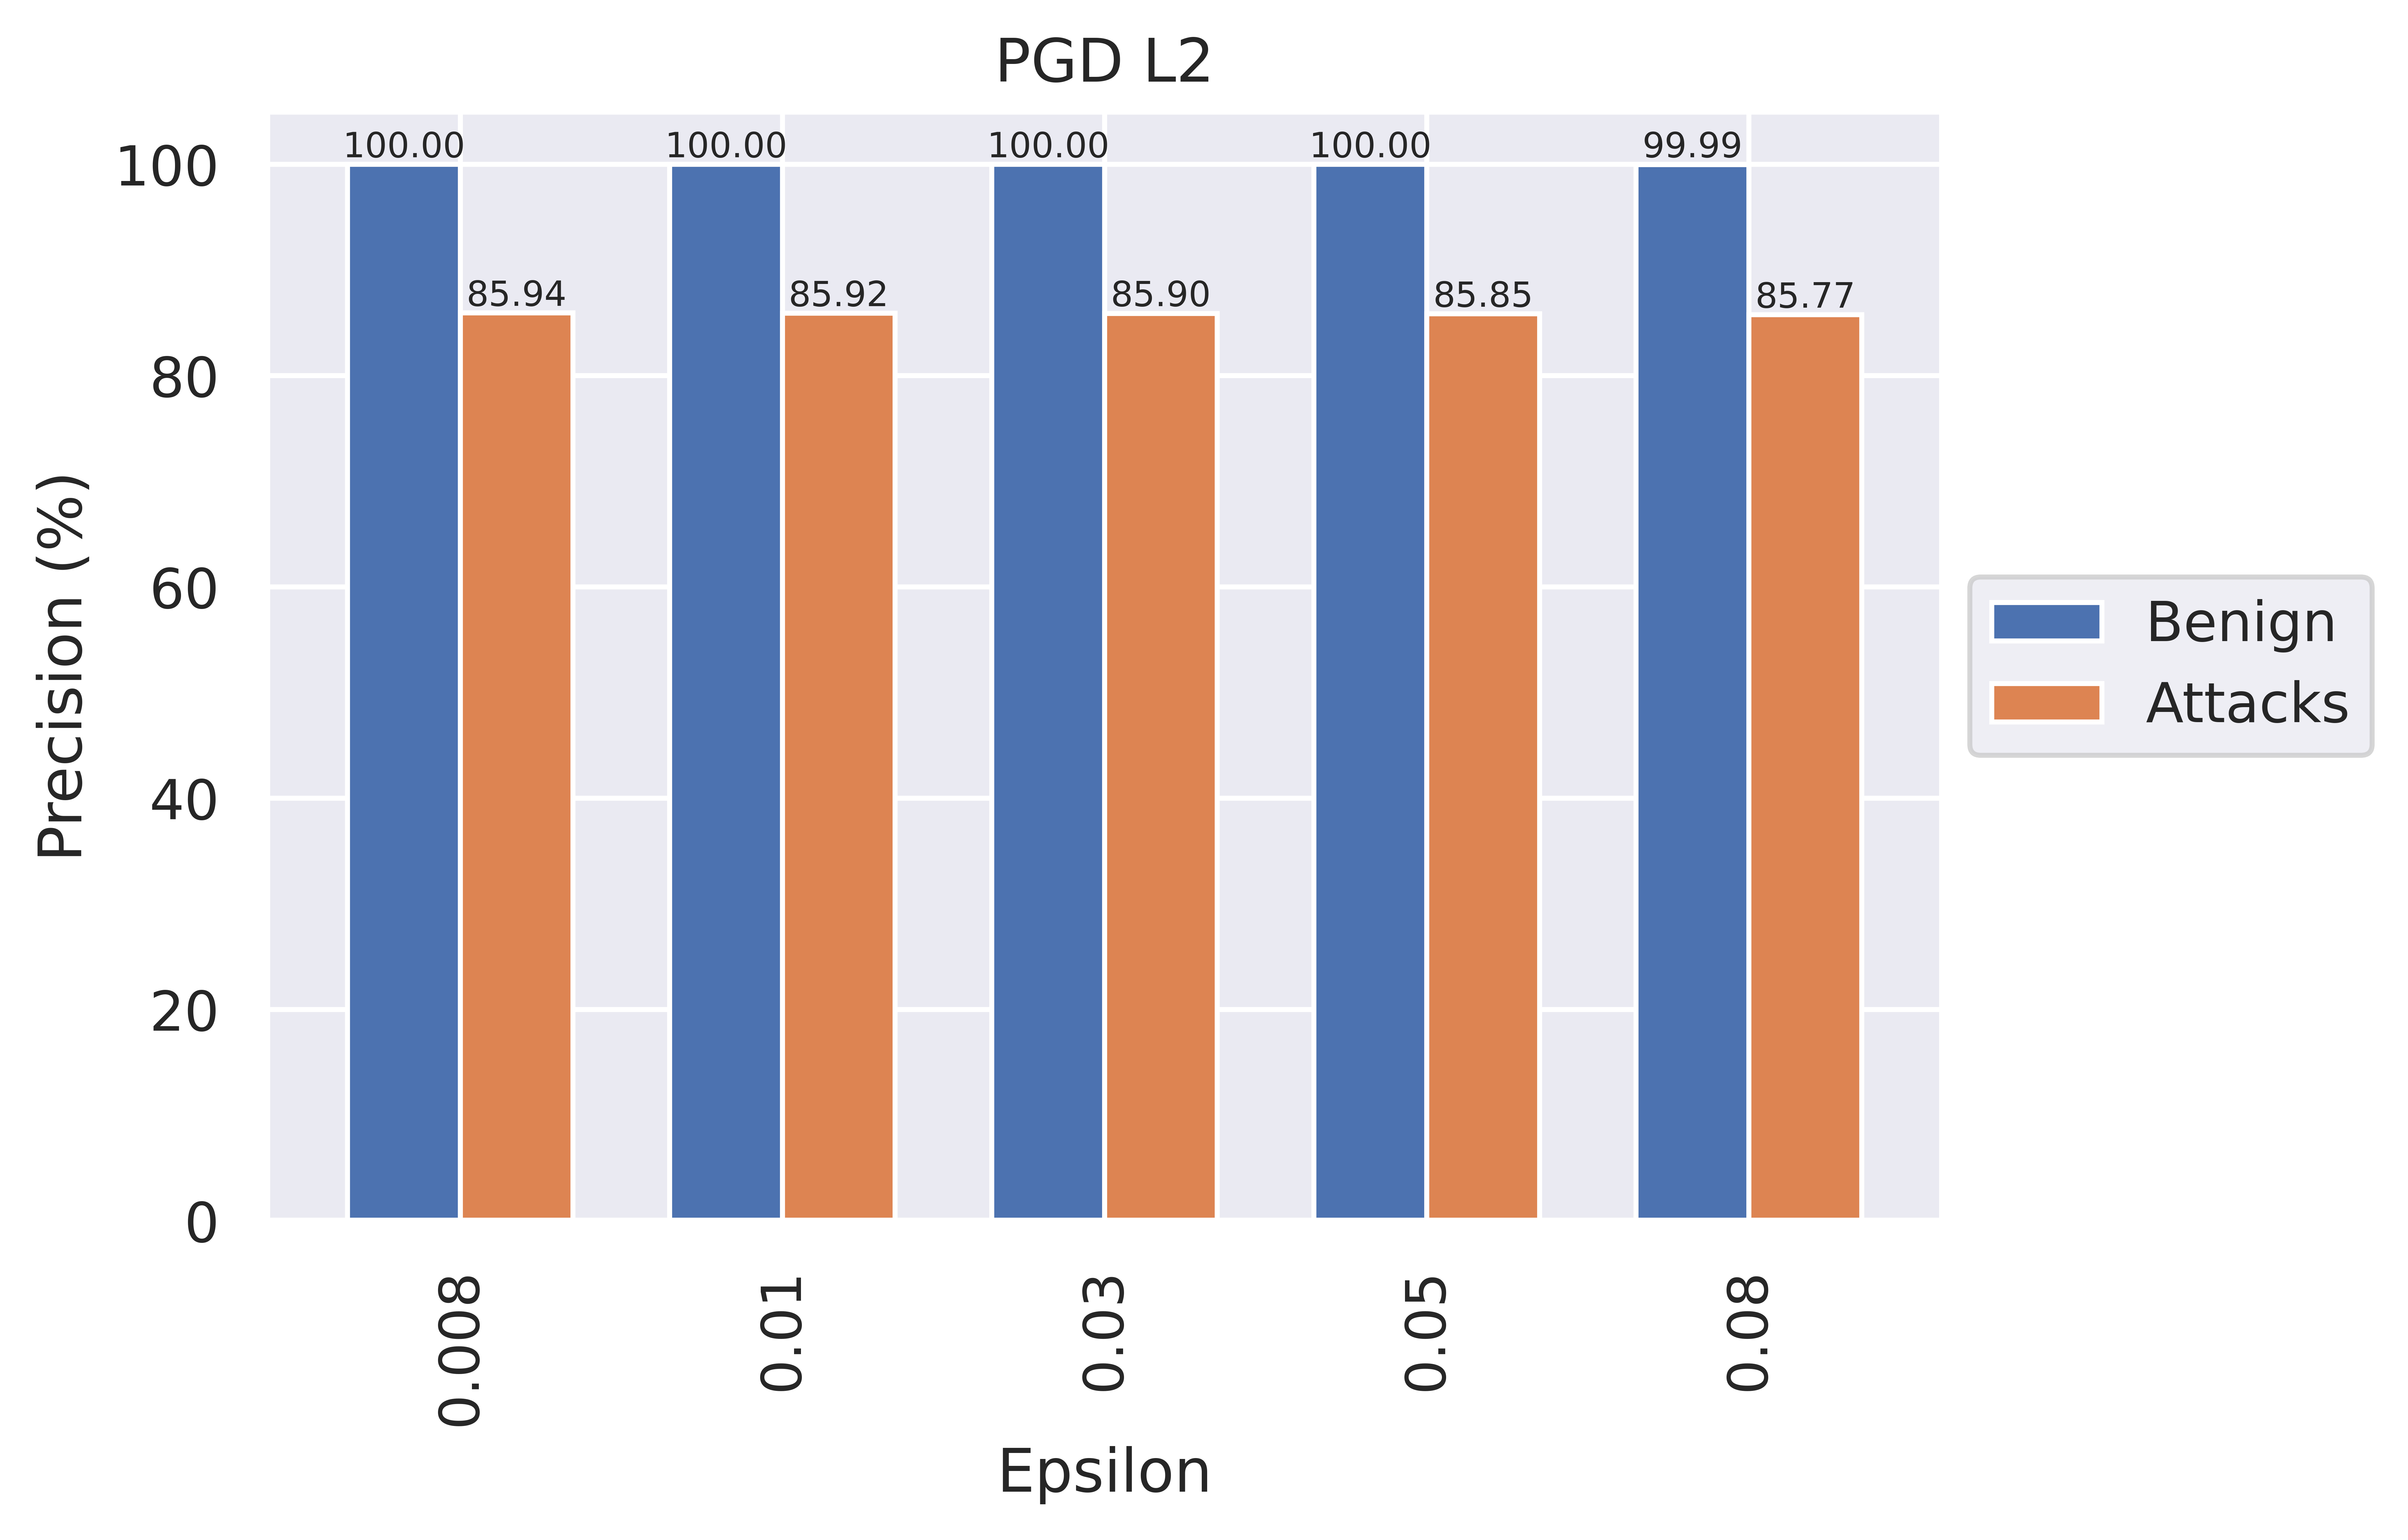
\includegraphics[width=\textwidth]{/home/wojtyla/Documentos/Artigo_2023/IJCNN_Suplementary/Figures//UNSW_Clean_PGD L2_bin_paper.png}
			%caption{Figure}
			\label{fig:2}
		\end{subfigure}
		\hfill
		\begin{subfigure}[b]{0.45\textwidth}
			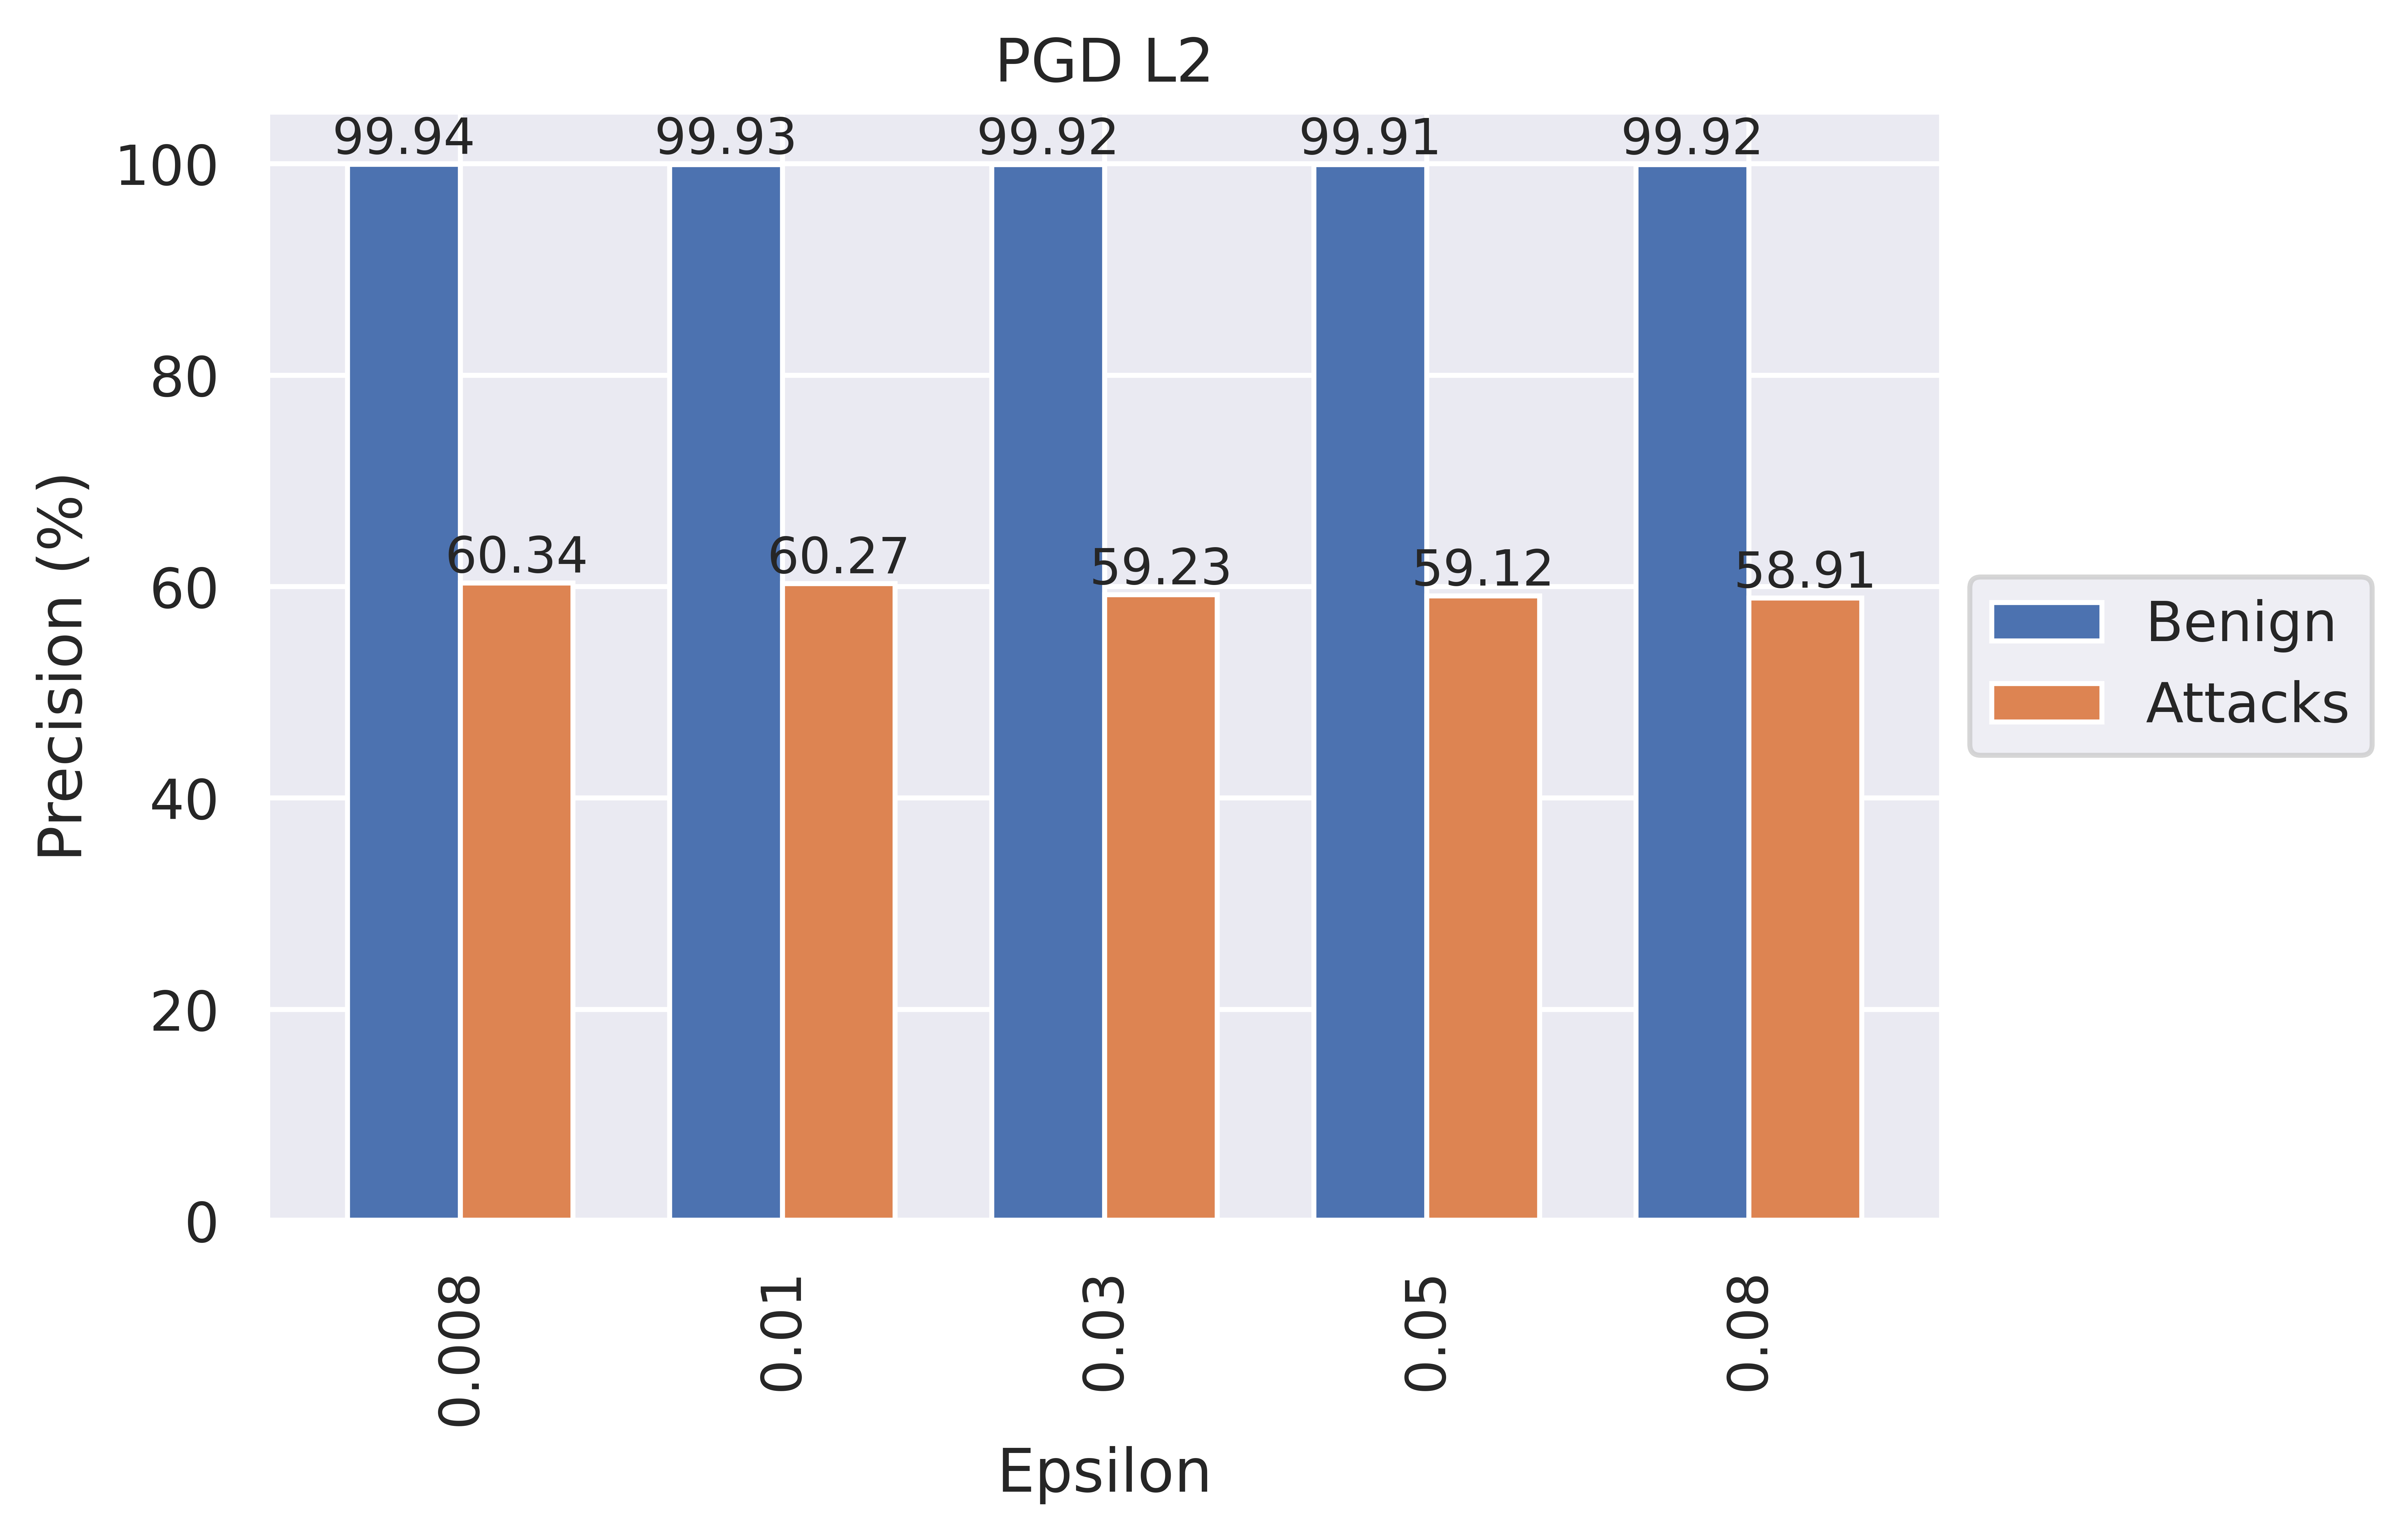
\includegraphics[width=\textwidth]{/home/wojtyla/Documentos/Artigo_2023/IJCNN_Suplementary/Figures///UNSW_IDS_PGD L2_bin_paper.png}
			%caption{Figure}
			\label{fig:5}
		\end{subfigure}
		
		\vskip\baselineskip
		
		\begin{subfigure}[b]{0.45\textwidth}
			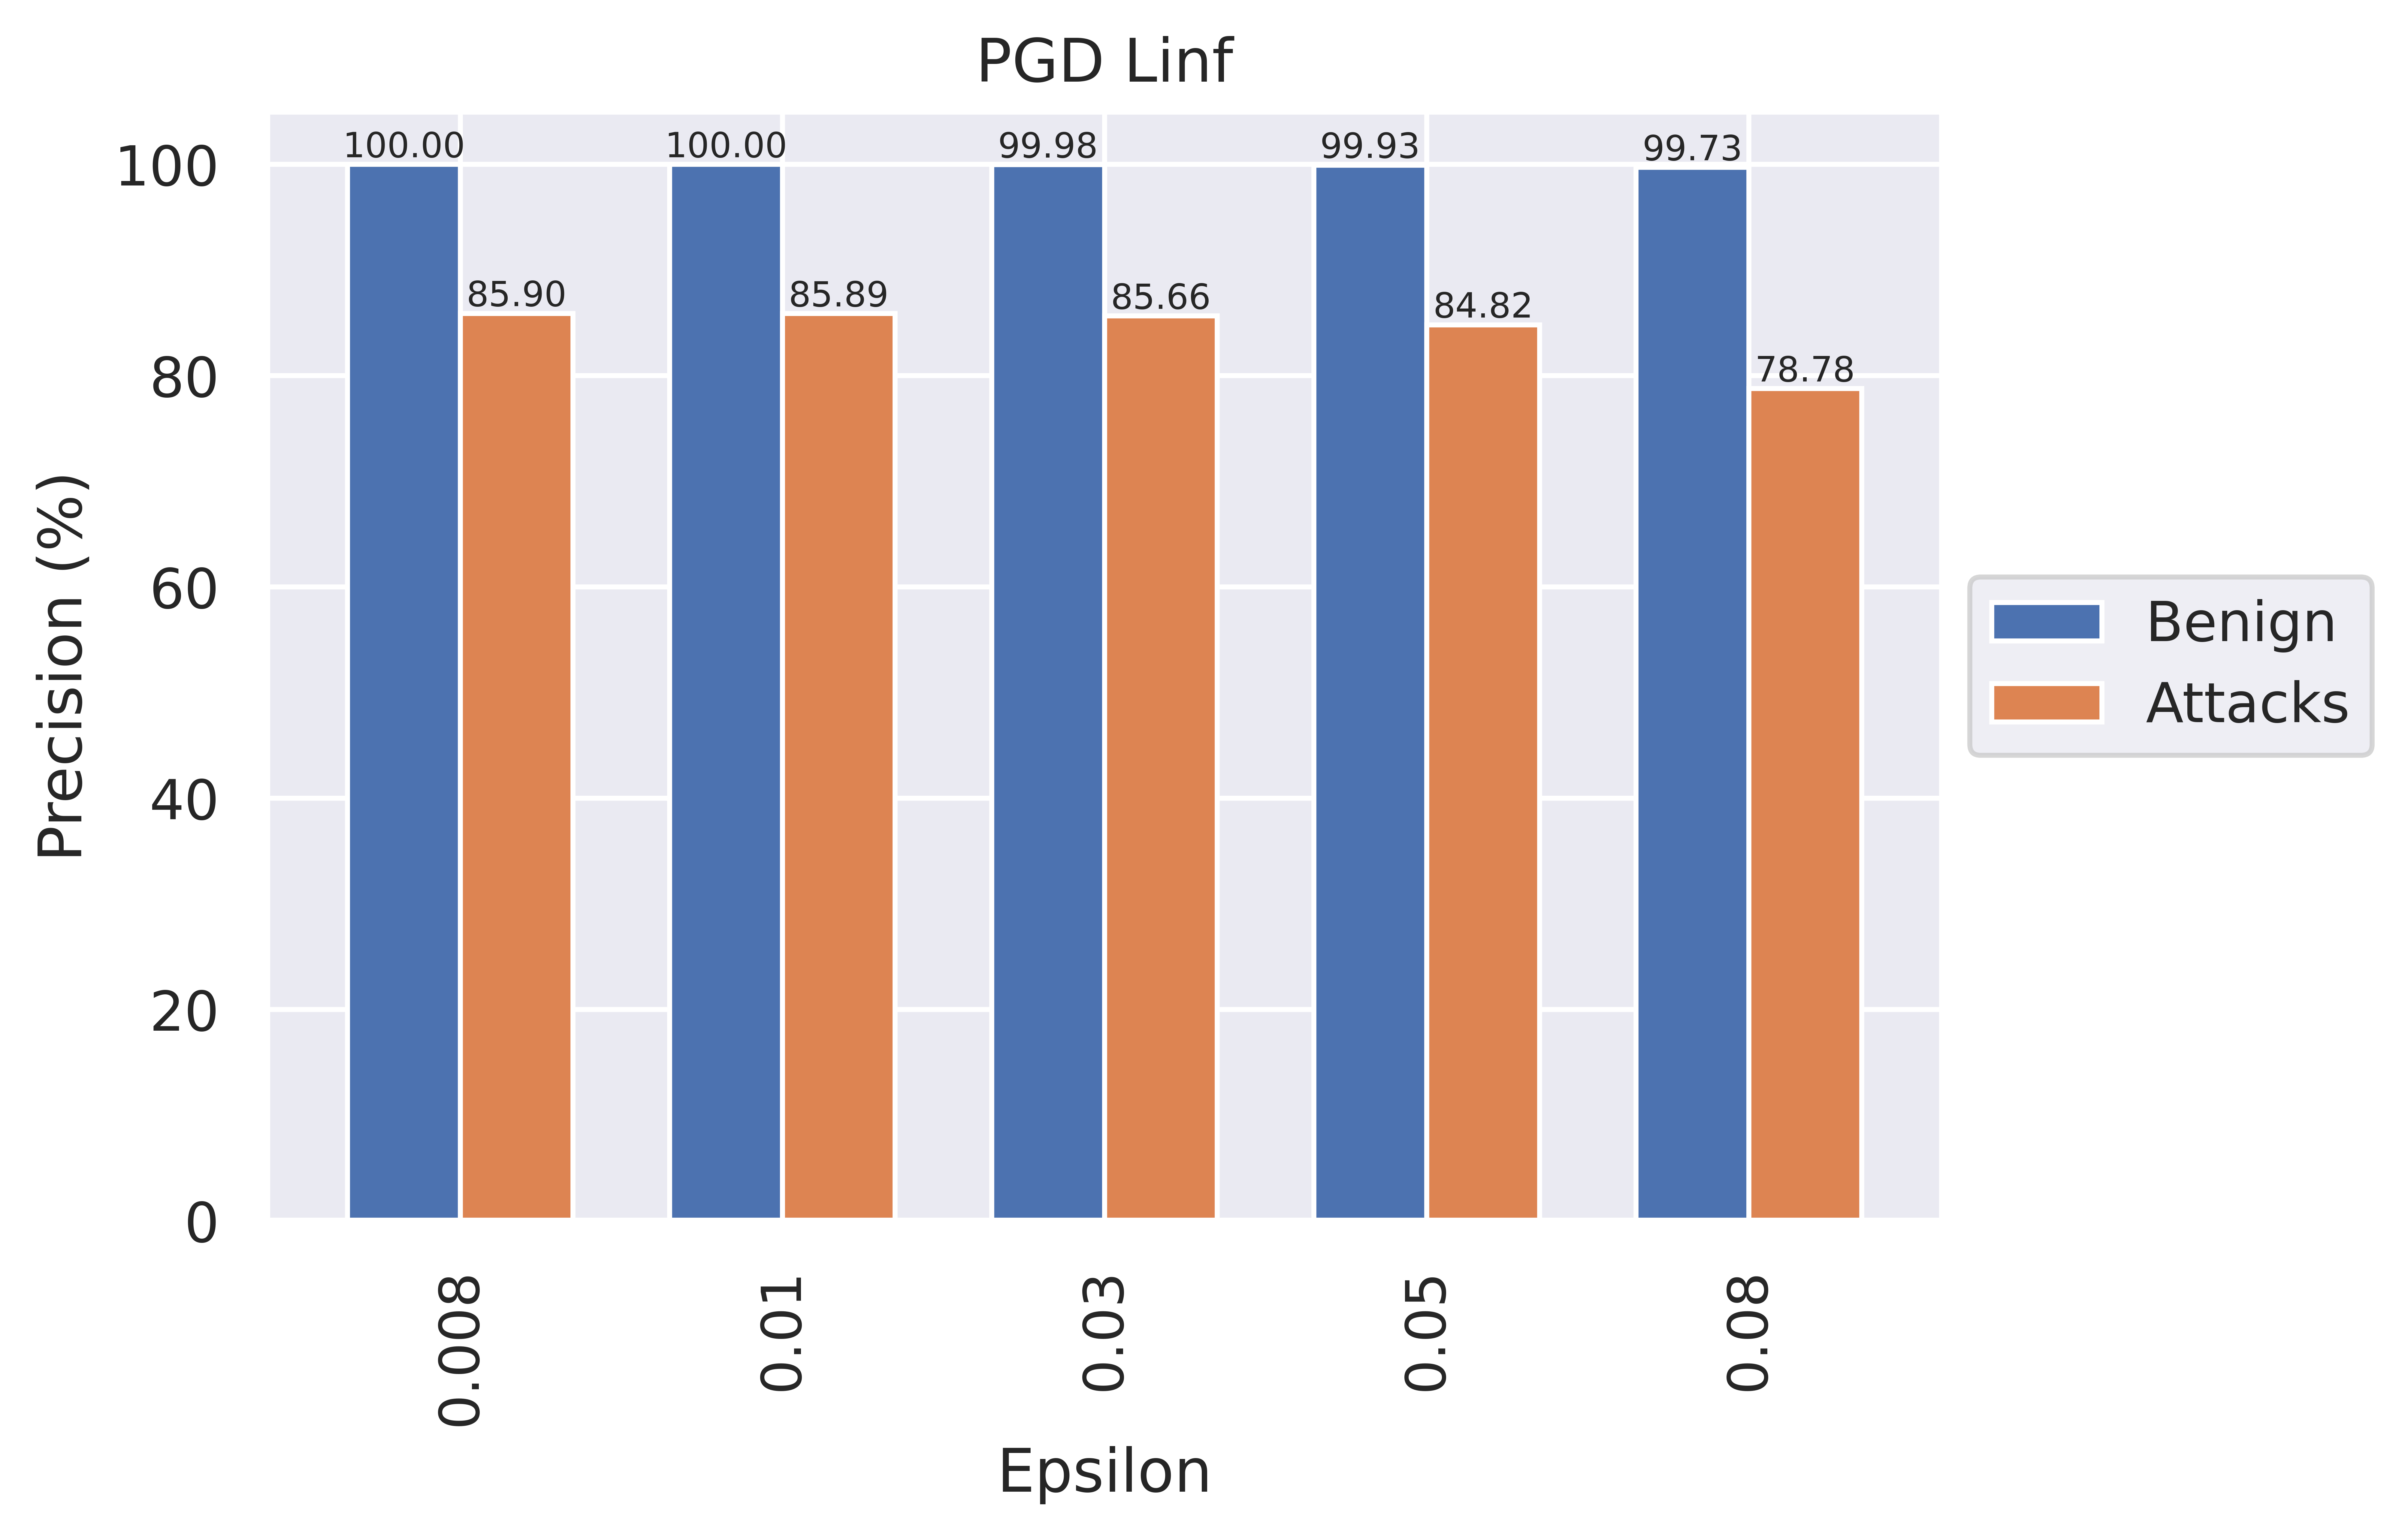
\includegraphics[width=\textwidth]{/home/wojtyla/Documentos/Artigo_2023/IJCNN_Suplementary/Figures//UNSW_Clean_PGD Linf_bin_paper.png}
			%caption{Figure}
			\label{fig:3}
		\end{subfigure}			
		\hfill
		\begin{subfigure}[b]{0.45\textwidth}
			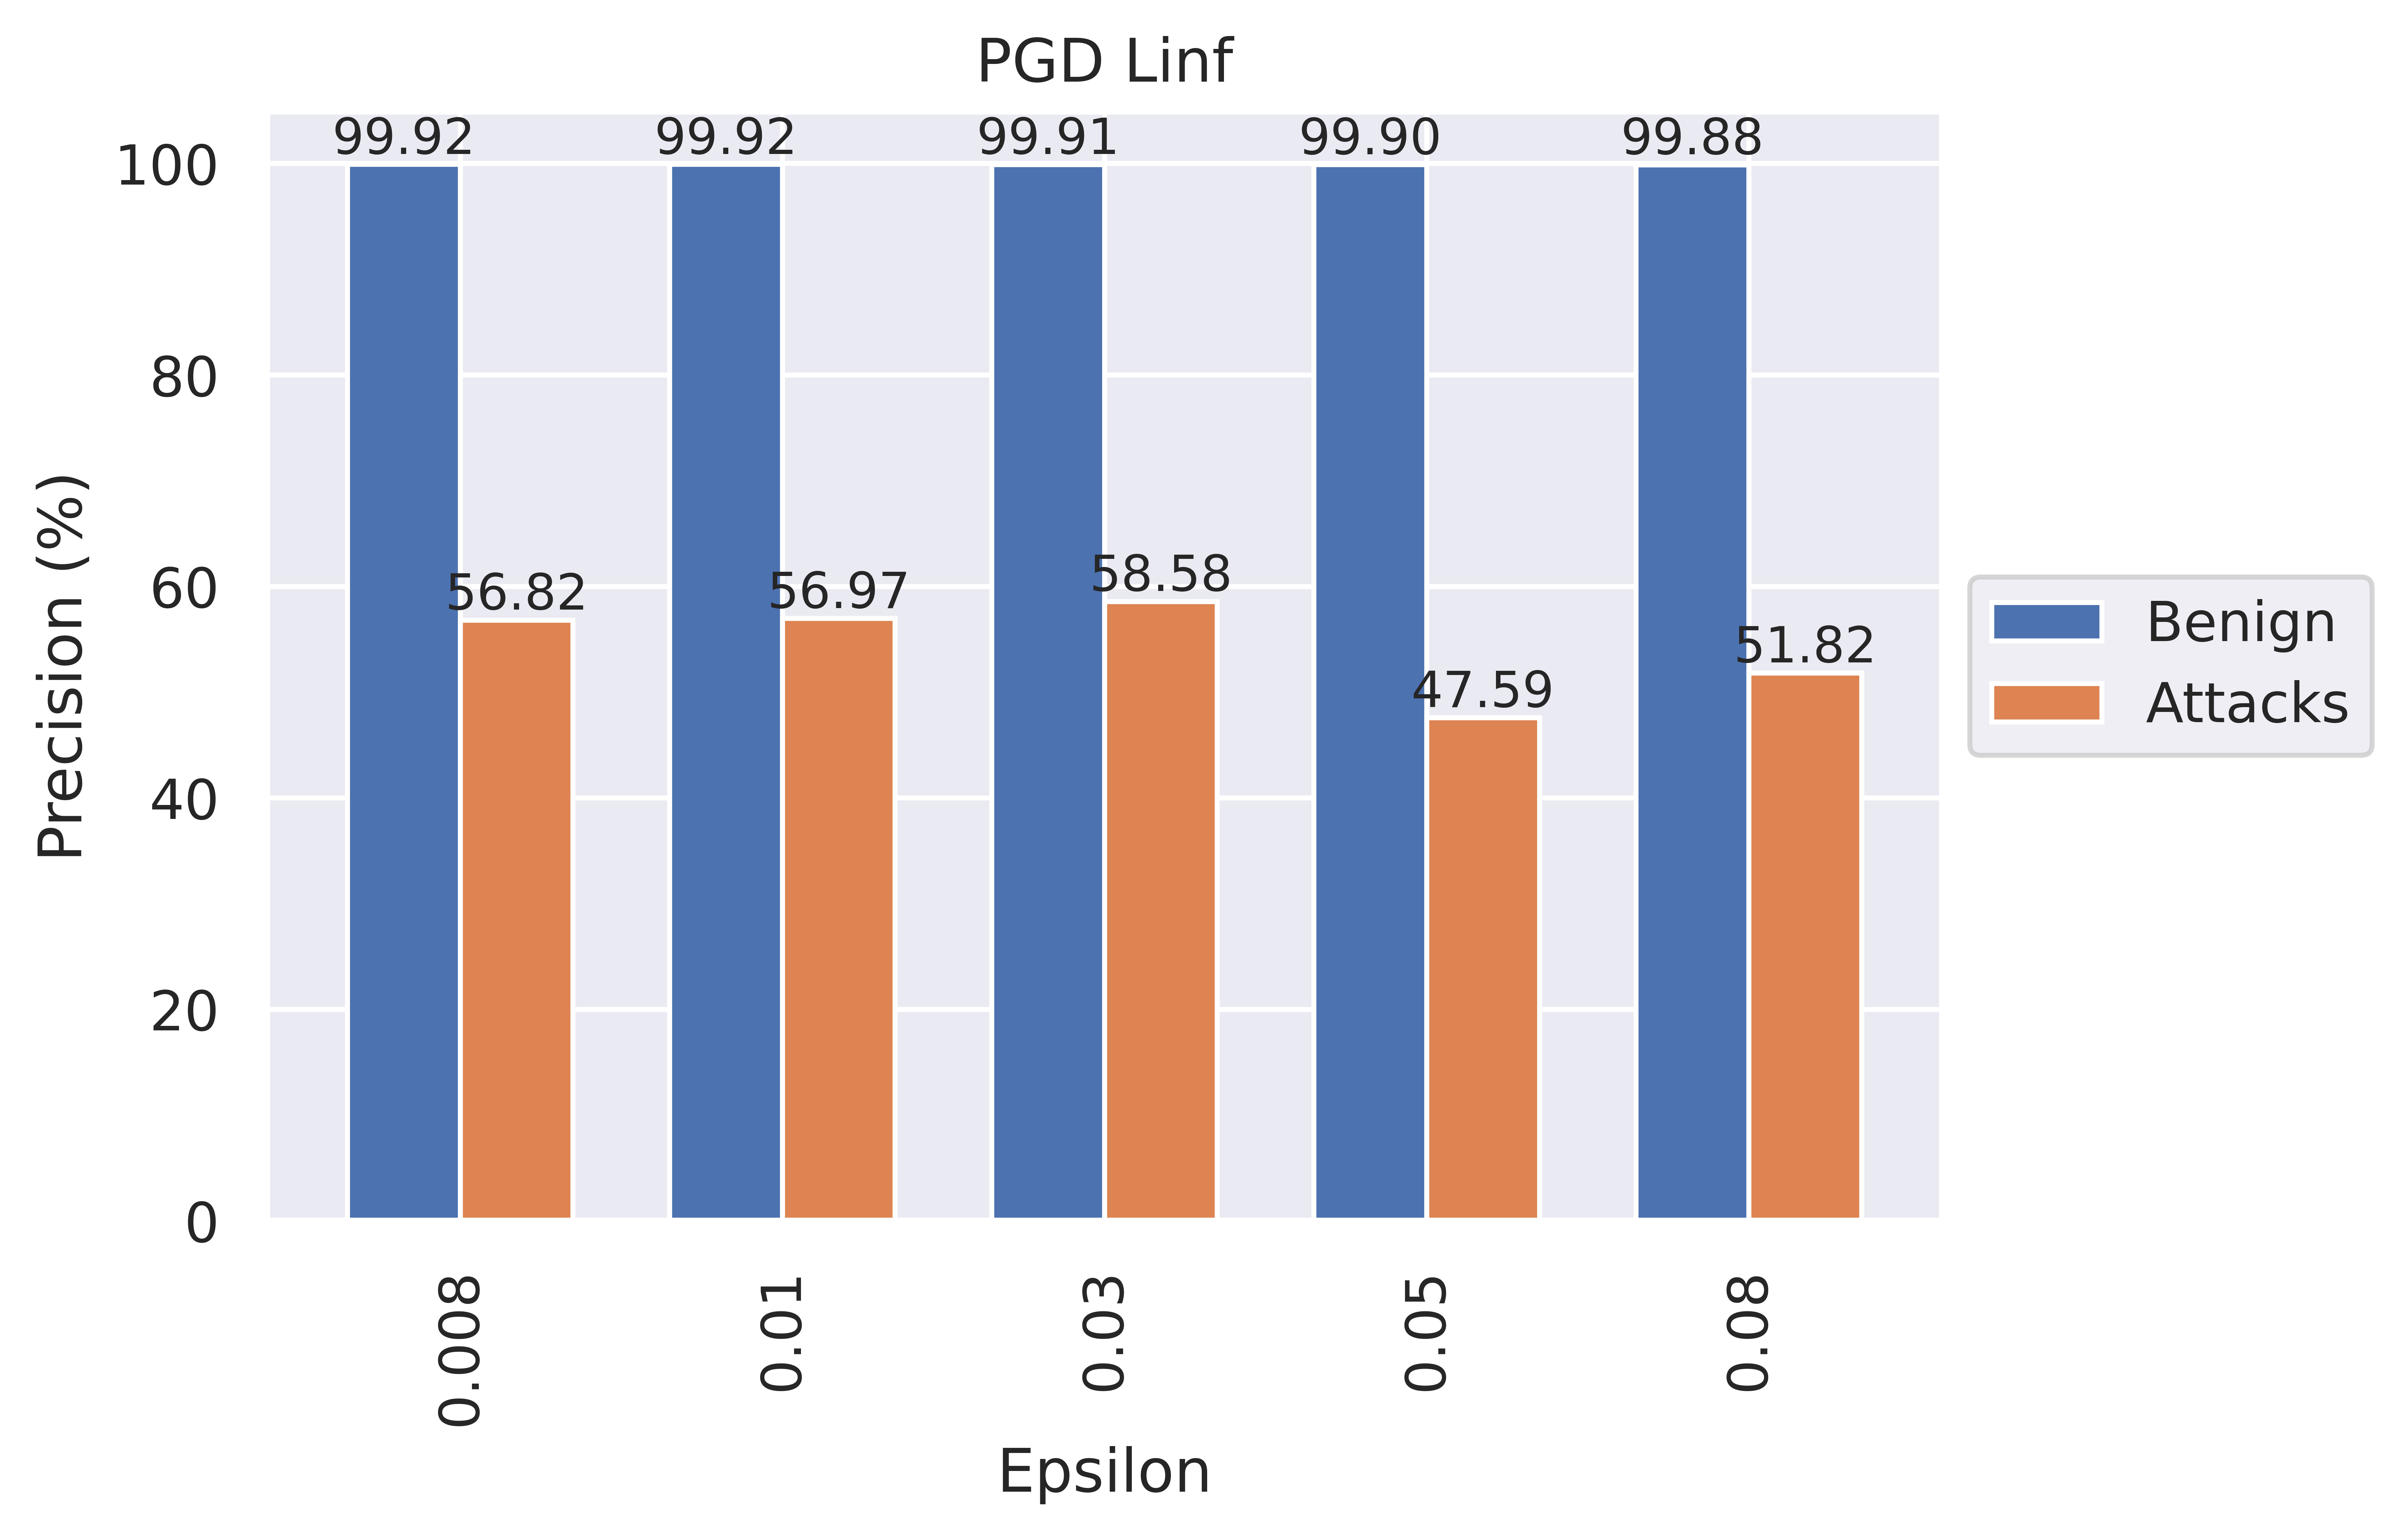
\includegraphics[width=\textwidth]{/home/wojtyla/Documentos/Artigo_2023/IJCNN_Suplementary/Figures///UNSW_IDS_PGD Linf_bin_paper.png}
			%caption{Figure}
			\label{fig:6}
		\end{subfigure}
		\caption{Plots for PGD-100 attack on binary models with UNSW-NB15.Left:EnC model; Right:EnIDS model.}
		\label{fig:unsw_pgd_bin}
	\end{figure}
	
	
	\begin{table}[H]
		\caption{PGD-100 attack against EnC and EnIDS for multiclass classification on the UNSW-NB15 dataset.}
		\small
		\setlength{\tabcolsep}{0.1pt}
		\centering
		\label{tab:unsw_multi_pgd}
		\hspace*{-1.7cm}
		\begin{tabular}{|c|c|c|c|c|c|c|c|c|c|c|c|c|c|c|c|c|c|}
			\hline
			\multirow{3}{*}{\textbf{Type}} & \multirow{3}{*}{\textbf{Norm}} & \multirow{3}{*}{\textbf{Metrics}} & \multicolumn{15}{c|}{\textbf{Epsilon ($\epsilon$)}
			} \\
			\cline{4-18}
			&  &  & \multicolumn{3}{c|}{\textbf{0.008}} & \multicolumn{3}{c|}{\textbf{0.01}} & \multicolumn{3}{c|}{\textbf{0.03}} & \multicolumn{3}{c|}{\textbf{0.05}} & \multicolumn{3}{c|}{\textbf{0.08}}
			\\
			\cline{4-18}
			&  &  & \textbf{\textsl{Normal}} & \textbf{\textsl{Recon.}} & \textbf{\textsl{Generic}} & \textbf{\textsl{Normal}} & \textbf{\textsl{Recon.}} & \textbf{\textsl{Generic}} & \textbf{\textsl{Normal}} & \textbf{\textsl{Recon.}} & \textbf{\textsl{Generic}} & \textbf{\textsl{Normal}} & \textbf{\textsl{Recon.}} & \textbf{\textsl{Generic}} & \textbf{\textsl{Normal}} & \textbf{\textsl{Recon.}} & \textbf{\textsl{Generic}}
			\\
			\hline
			\multirow{9}{*}
			{EnC} & \multirow{3}{*}{\( \ell_1 \)} & Precision & 100.00 & 80.10 & 100.00 & 100.00 & 80.41 & 100.00 & 100.00 & 78.12 & 100.00 & 100.00 & 75.71 & 100.00 & 100.00 & 58.23 & 99.85
			\\
			
			&  & Recall & 99.52 & 90.34 & 91.56 & 99.52 & 89.77 & 91.56 & 99.52 & 85.23 & 91.56 & 99.52 & 75.28 & 91.49 & 99.52 & 41.19 & 90.89
			\\
			
			&  & ROC-AUC & 99.96 & 99.98 & 99.97 & 99.96 & 99.98 & 99.97 & 99.95 & 99.97 & 99.97 & 99.95 & 99.95 & 99.97 & 99.95 & 99.88 & 99.96
			\\
			\cline{2-18}
			& \multirow{3}{*}{\( \ell_2 \)} & Precision & 100.00 & 79.74 & 100.00 & 100.00 & 78.41 & 100.00 & 100.00 & 53.02 & 99.93 & 100.00 & 24.85 & 99.71 & 100.00 & 9.15 & 94.98
			\\
			
			&  & Recall & 99.52 & 88.35 & 91.56 & 99.52 & 86.65 & 91.56 & 99.52 & 32.39 & 91.36 & 99.52 & 11.93 & 90.56 & 99.52 & 3.98 & 90.62
			\\
			
			&  & ROC-AUC & 99.95 & 99.98 & 99.97 & 99.95 & 99.98 & 99.97 & 99.94 & 99.84 & 99.96 & 99.93 & 99.67 & 99.95 & 99.90 & 99.44 & 99.93
			\\
			\cline{2-18}
			& \multirow{3}{*}{\( \ell_\infty \)} & Precision & 100.00 & 72.73 & 100.00 & 100.00 & 53.55 & 100.00 & 100.00 & 23.49 & 99.63 & 100.00 & 19.20 & 93.22 & 99.99 & 14.94 & 70.27
			\\
			
			&  & Recall & 99.52 & 70.45 & 91.49 & 99.52 & 32.10 & 91.42 & 99.52 & 11.08 & 89.89 & 99.52 & 6.82 & 87.77 & 99.53 & 6.53 & 24.20
			\\
			
			&  & ROC-AUC & 99.94 & 99.94 & 99.96 & 99.94 & 99.85 & 99.96 & 99.91 & 99.36 & 99.94 & 99.87 & 99.18 & 99.90 & 99.72 & 98.97 & 99.15
			\\
			\hline
			\multirow{9}{*}
			{EnIDS}  & \multirow{3}{*}{\( \ell_1 \)} & Precision & \cellcolor{blue!20}100.00 & 50.97 & 97.86 & \cellcolor{blue!20}100.00 & 48.08 & 97.65 & \cellcolor{blue!20}100.00 & 40.00 & 97.55 & \cellcolor{blue!20}100.00 & 34.03 & 94.11 & \cellcolor{blue!20}100.00 & 30.10 & 87.41
			\\
			
			&  & Recall & \cellcolor{yellow!50}99.61 & 59.94 & 91.16 & \cellcolor{yellow!50}99.61 & 56.82 & 91.16 & \cellcolor{yellow!50}99.61 & 52.84 & 87.43 & 99.61 & 51.14 & 88.23 & \cellcolor{yellow!50}99.61 & \cellcolor{yellow!50}51.14 & 86.30
			\\
			
			&  & ROC-AUC & 99.93 & 99.88 & 99.95 & 99.93 & 99.87 & 99.95 & 99.93 & 99.85 & 99.94 & 99.92 & 99.80 & 99.93 & 99.92 & 99.78 & 99.93
			\\
			\cline{2-18}
			& \multirow{3}{*}{\( \ell_2 \)} & Precision & \cellcolor{blue!20}100.00 & 43.55 & 96.52 & \cellcolor{blue!20}100.00 & 38.48 & 95.76 & \cellcolor{blue!20}100.00 & 28.24 & 85.59 & \cellcolor{blue!20}100.00 & 22.96 & 77.08 & 100.00 & 18.70 & 75.20
			\\
			
			&  & Recall & \cellcolor{yellow!50}99.61 & 50.85 & 86.64 & 99.61 & 46.02 & 85.57 & \cellcolor{yellow!50}99.61 & \cellcolor{yellow!50}42.05 & 81.78 & 99.61 & \cellcolor{yellow!50}40.06 & 72.67 & \cellcolor{yellow!50}99.61 & \cellcolor{yellow!50}33.52 & 55.25
			\\
			
			&  & ROC-AUC & 99.93 & 99.86 & 99.94 & 99.93 & 99.84 & 99.93 & 99.91 & 99.74 & 99.90 & 99.89 & \cellcolor{yellow!50}99.71 & 99.87 & 99.88 & \cellcolor{yellow!50}99.65 & 99.83
			\\
			\cline{2-18}
			& \multirow{3}{*}{\( \ell_\infty \)} & Precision & 100.00 & 30.00 & 78.73 & 100.00 & 29.53 & 84.57 & 100.00 & 18.37 & 70.42 & 100.00 & 16.54 & 68.05 & 100.00 & 16.87 & 62.34
			\\
			
			&  & Recall & \cellcolor{yellow!50}99.61 & 39.20 & 69.15 & \cellcolor{yellow!50}99.61 & 38.92 & 63.03 & \cellcolor{yellow!50}99.61 & \cellcolor{yellow!50}30.68 & 45.28 & \cellcolor{yellow!50}99.61 & \cellcolor{yellow!50}30.11 & 41.36 & \cellcolor{yellow!50}99.61 & \cellcolor{yellow!50}31.82 & \cellcolor{yellow!50}42.15
			\\
			
			&  & ROC-AUC & 99.88 & 99.77 & 99.85 & 99.86 & 99.75 & 99.84 & 99.87 & 99.63 & 99.81 & 99.88 & 99.61 & 99.77 & 99.88 & 99.59 & 99.78
			\\
			\hline
		\end{tabular}		
	\end{table}
	
	
	\begin{figure}[H]
		\centering
		\begin{subfigure}[b]{0.45\textwidth}
			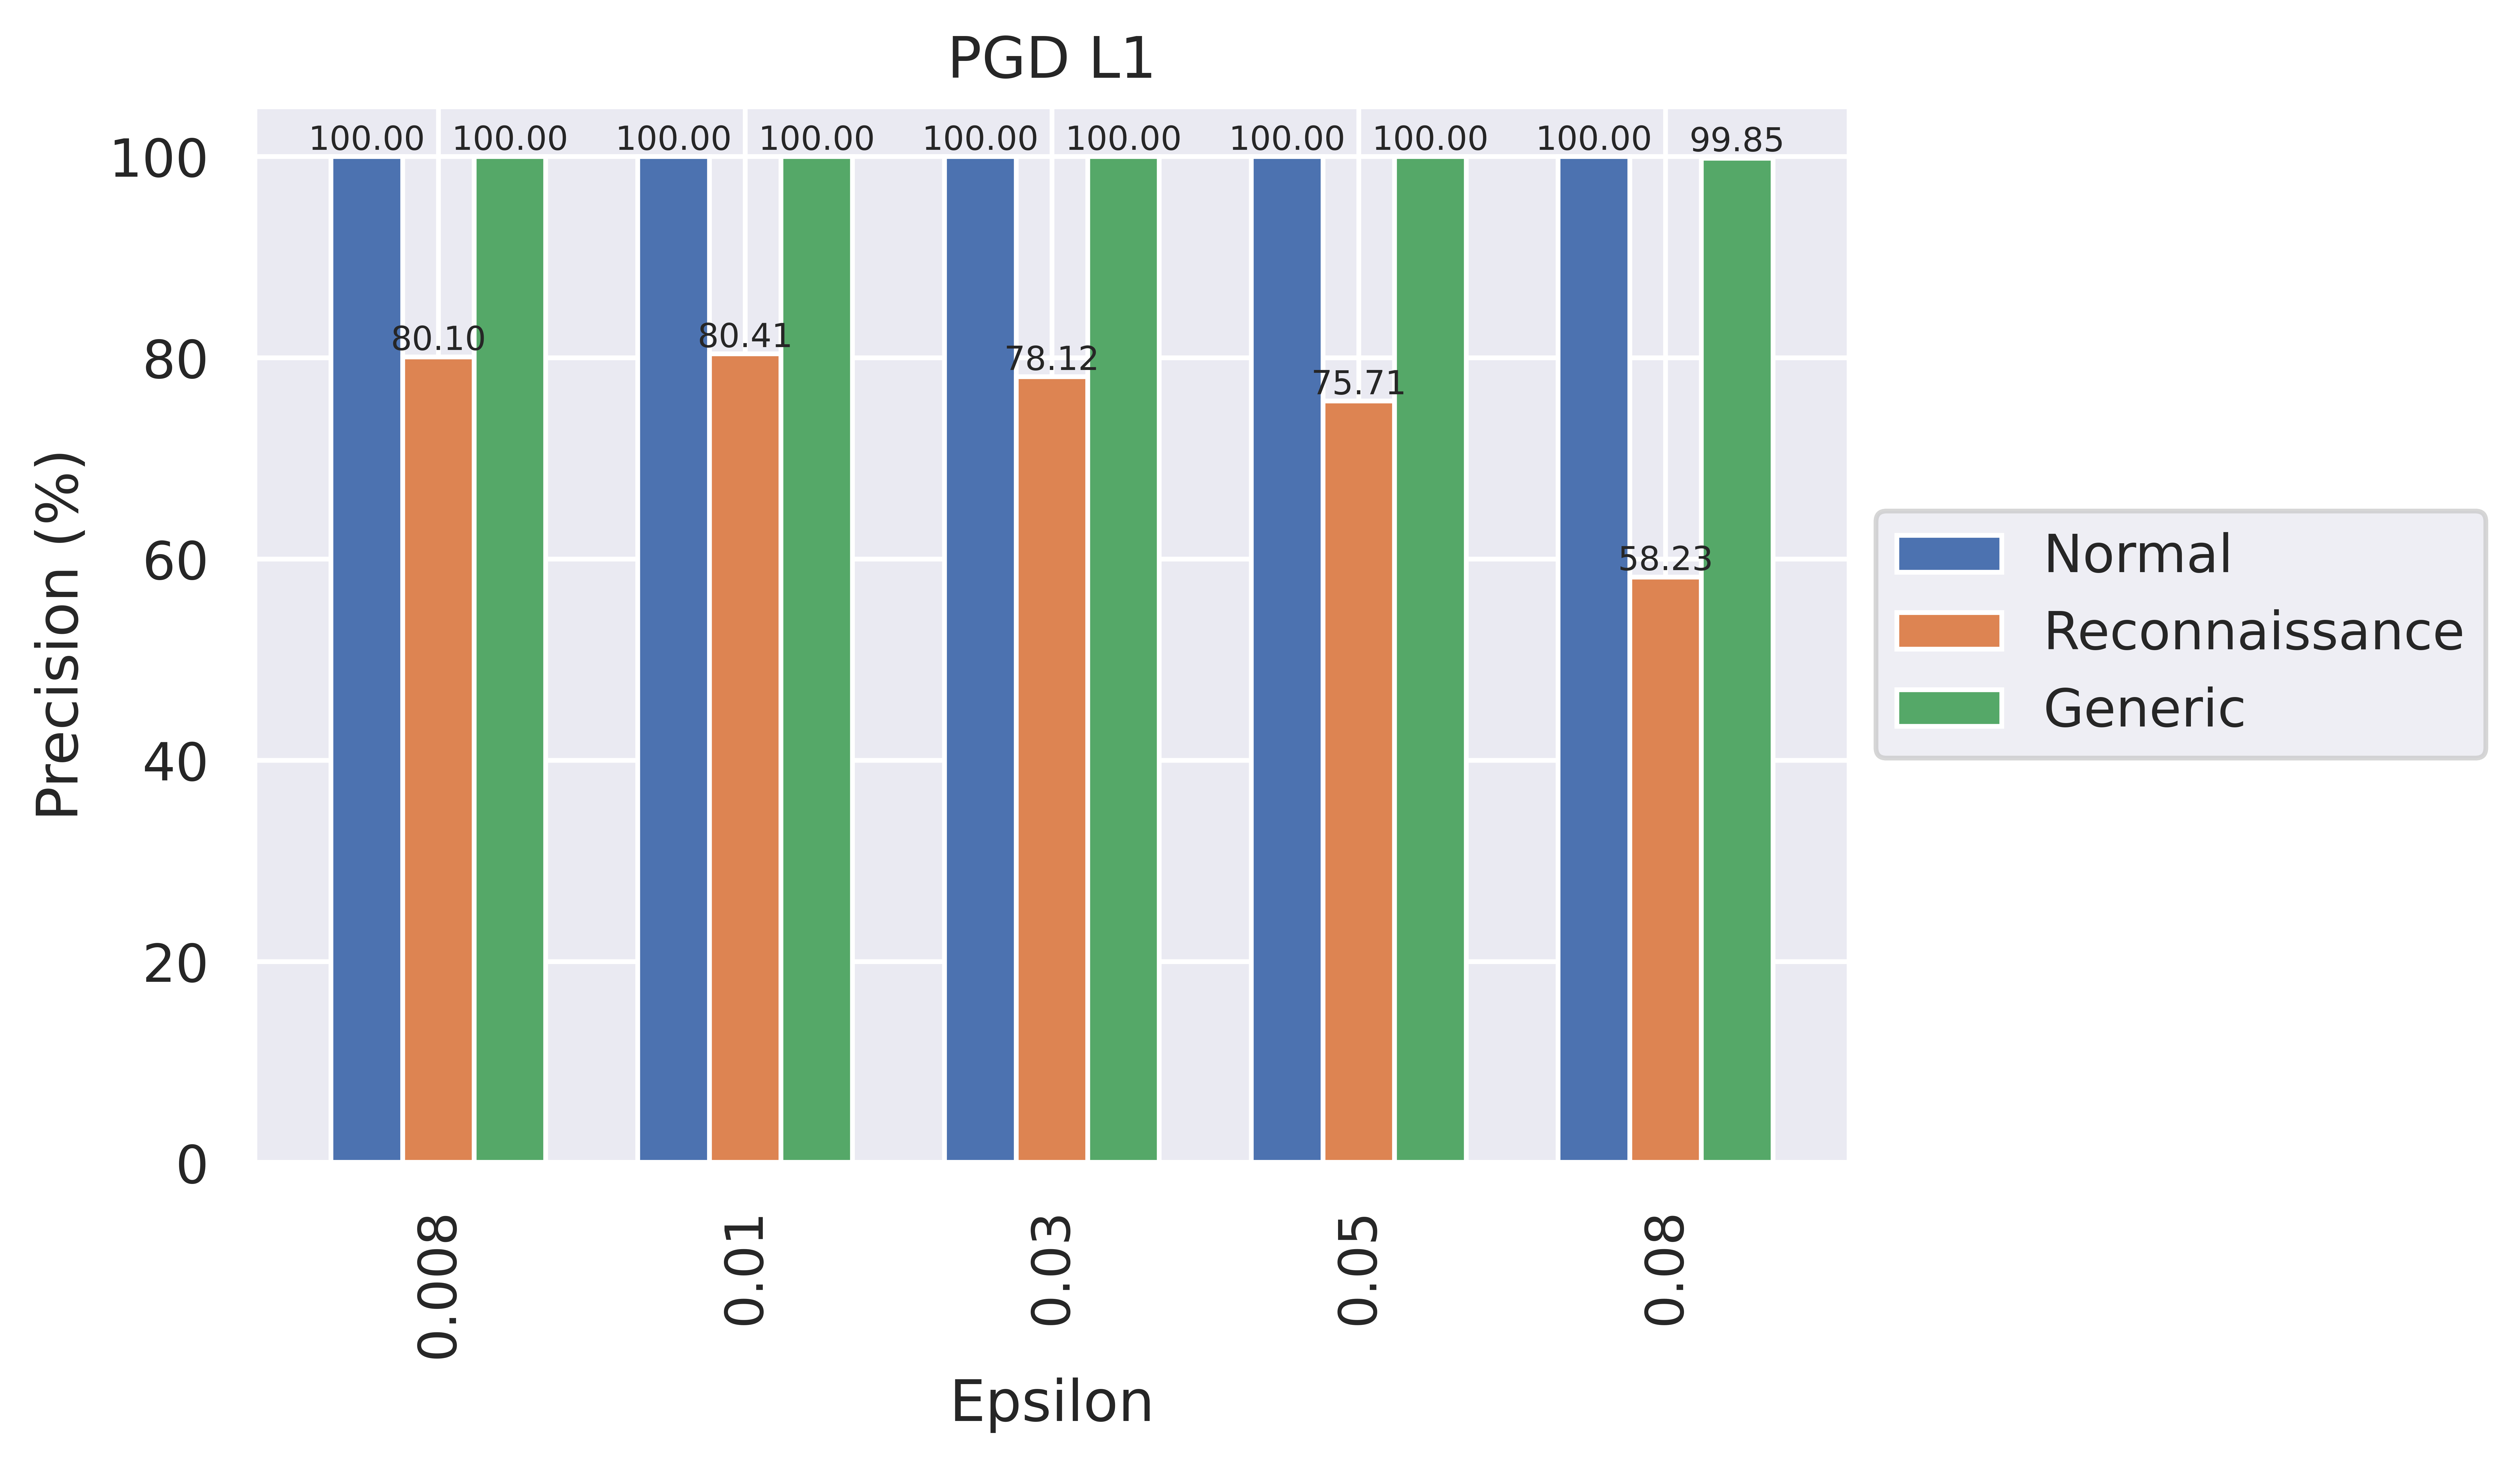
\includegraphics[width=\textwidth]{/home/wojtyla/Documentos/Artigo_2023/IJCNN_Suplementary/Figures/UNSW_Clean_PGD L1_multi_paper.png}
			%caption{Figure}
			\label{fig:1}
		\end{subfigure}
		\hfill
		\begin{subfigure}[b]{0.45\textwidth}
			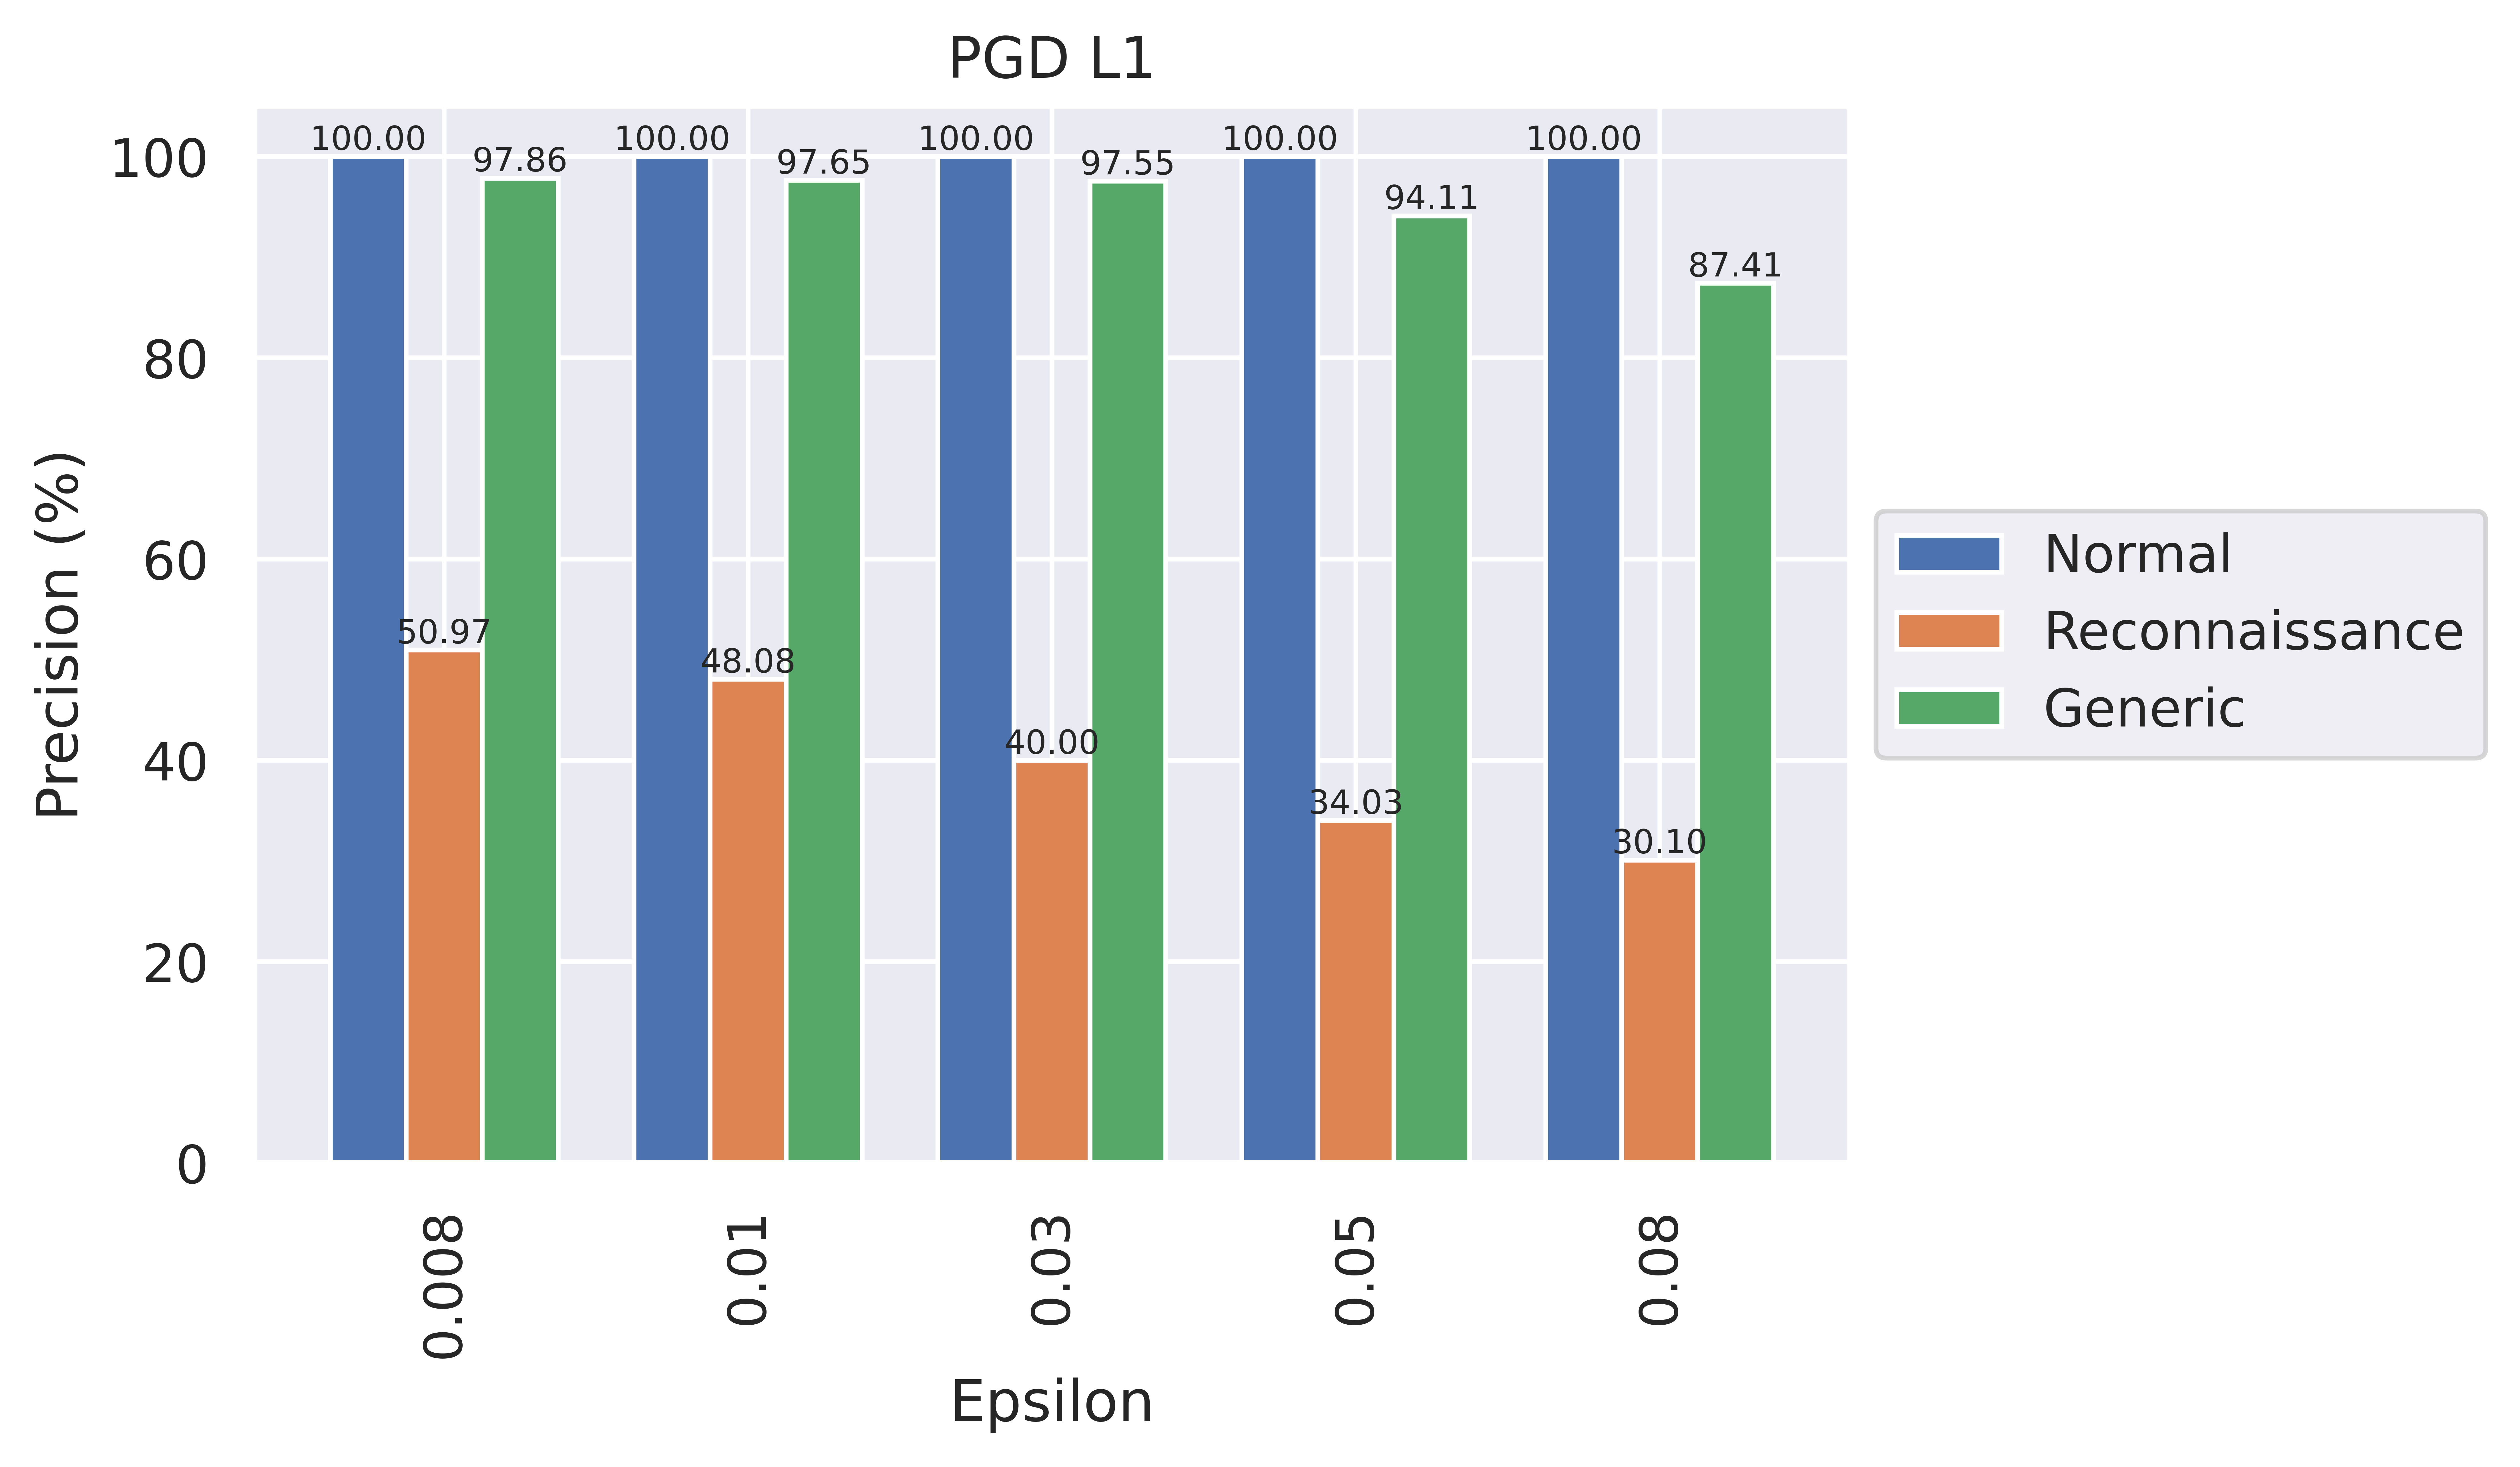
\includegraphics[width=\textwidth]{/home/wojtyla/Documentos/Artigo_2023/IJCNN_Suplementary/Figures//UNSW_IDS_PGD L1_multi_paper.png}
			%caption{Figure}
			\label{fig:4}
		\end{subfigure}
		\vskip\baselineskip
		\begin{subfigure}[b]{0.45\textwidth}
			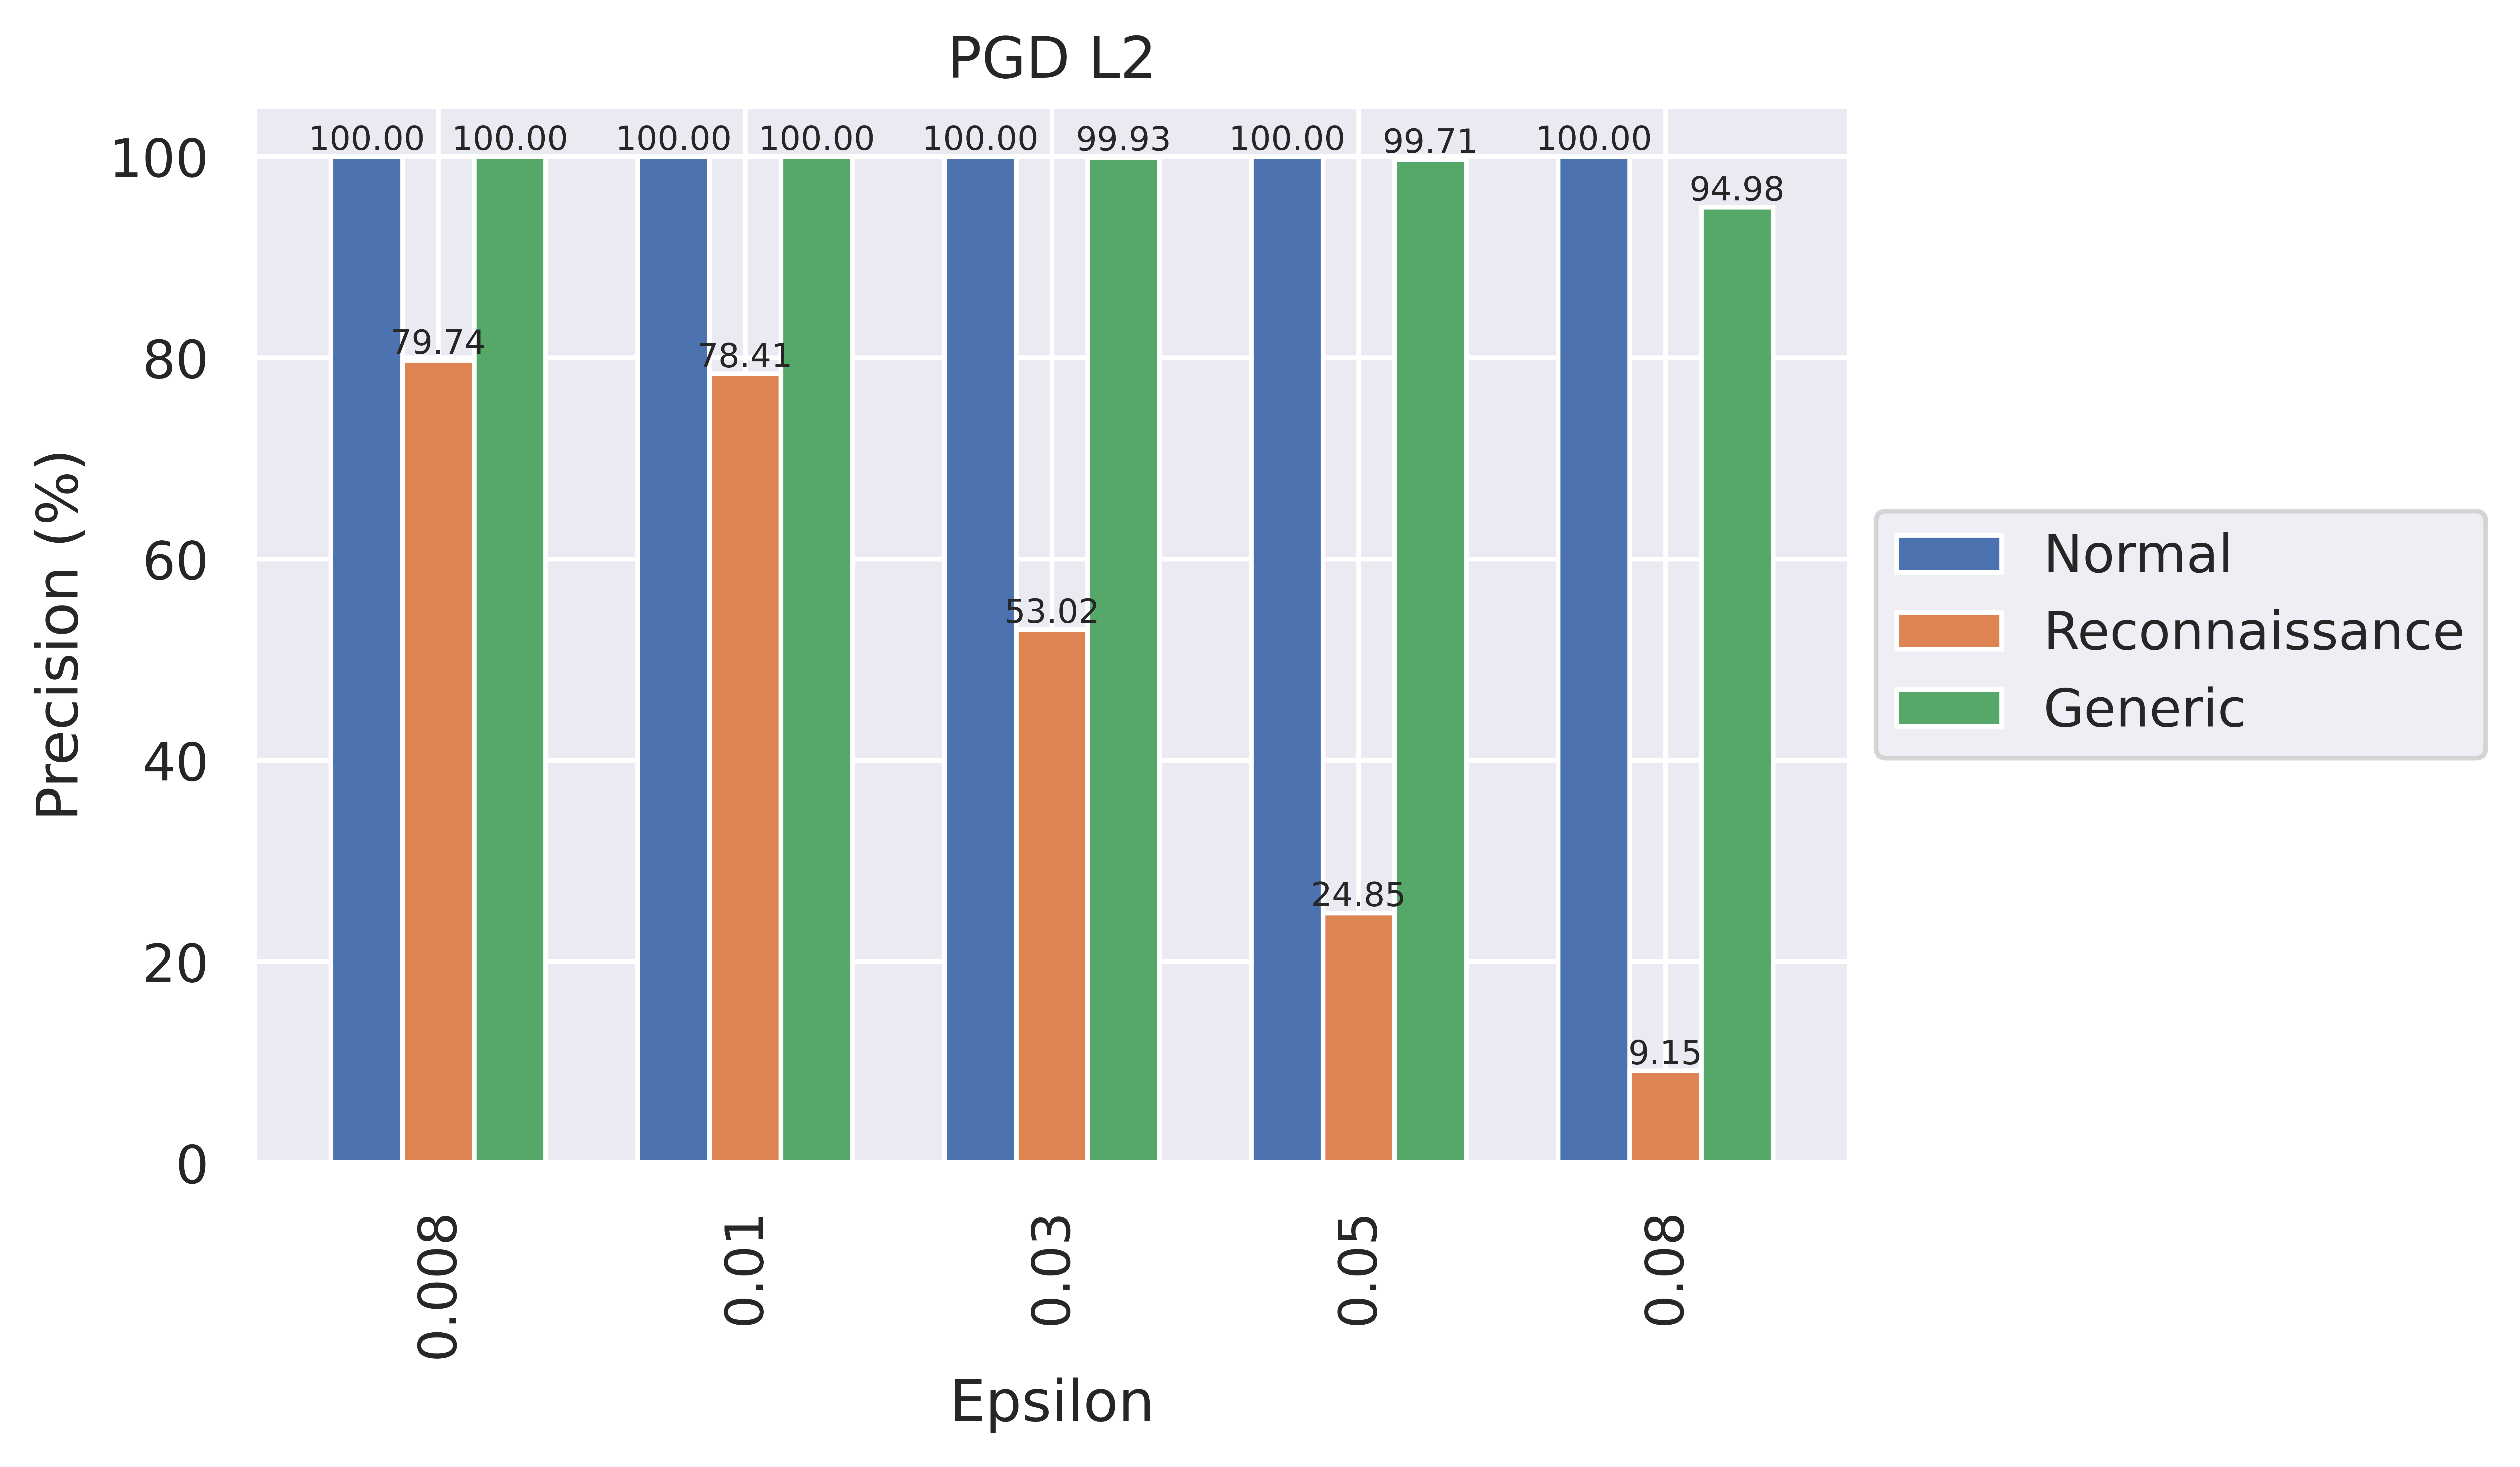
\includegraphics[width=\textwidth]{/home/wojtyla/Documentos/Artigo_2023/IJCNN_Suplementary/Figures/UNSW_Clean_PGD L2_multi_paper.png}
			%caption{Figure}
			\label{fig:2}
		\end{subfigure}
		\hfill
		\begin{subfigure}[b]{0.45\textwidth}
			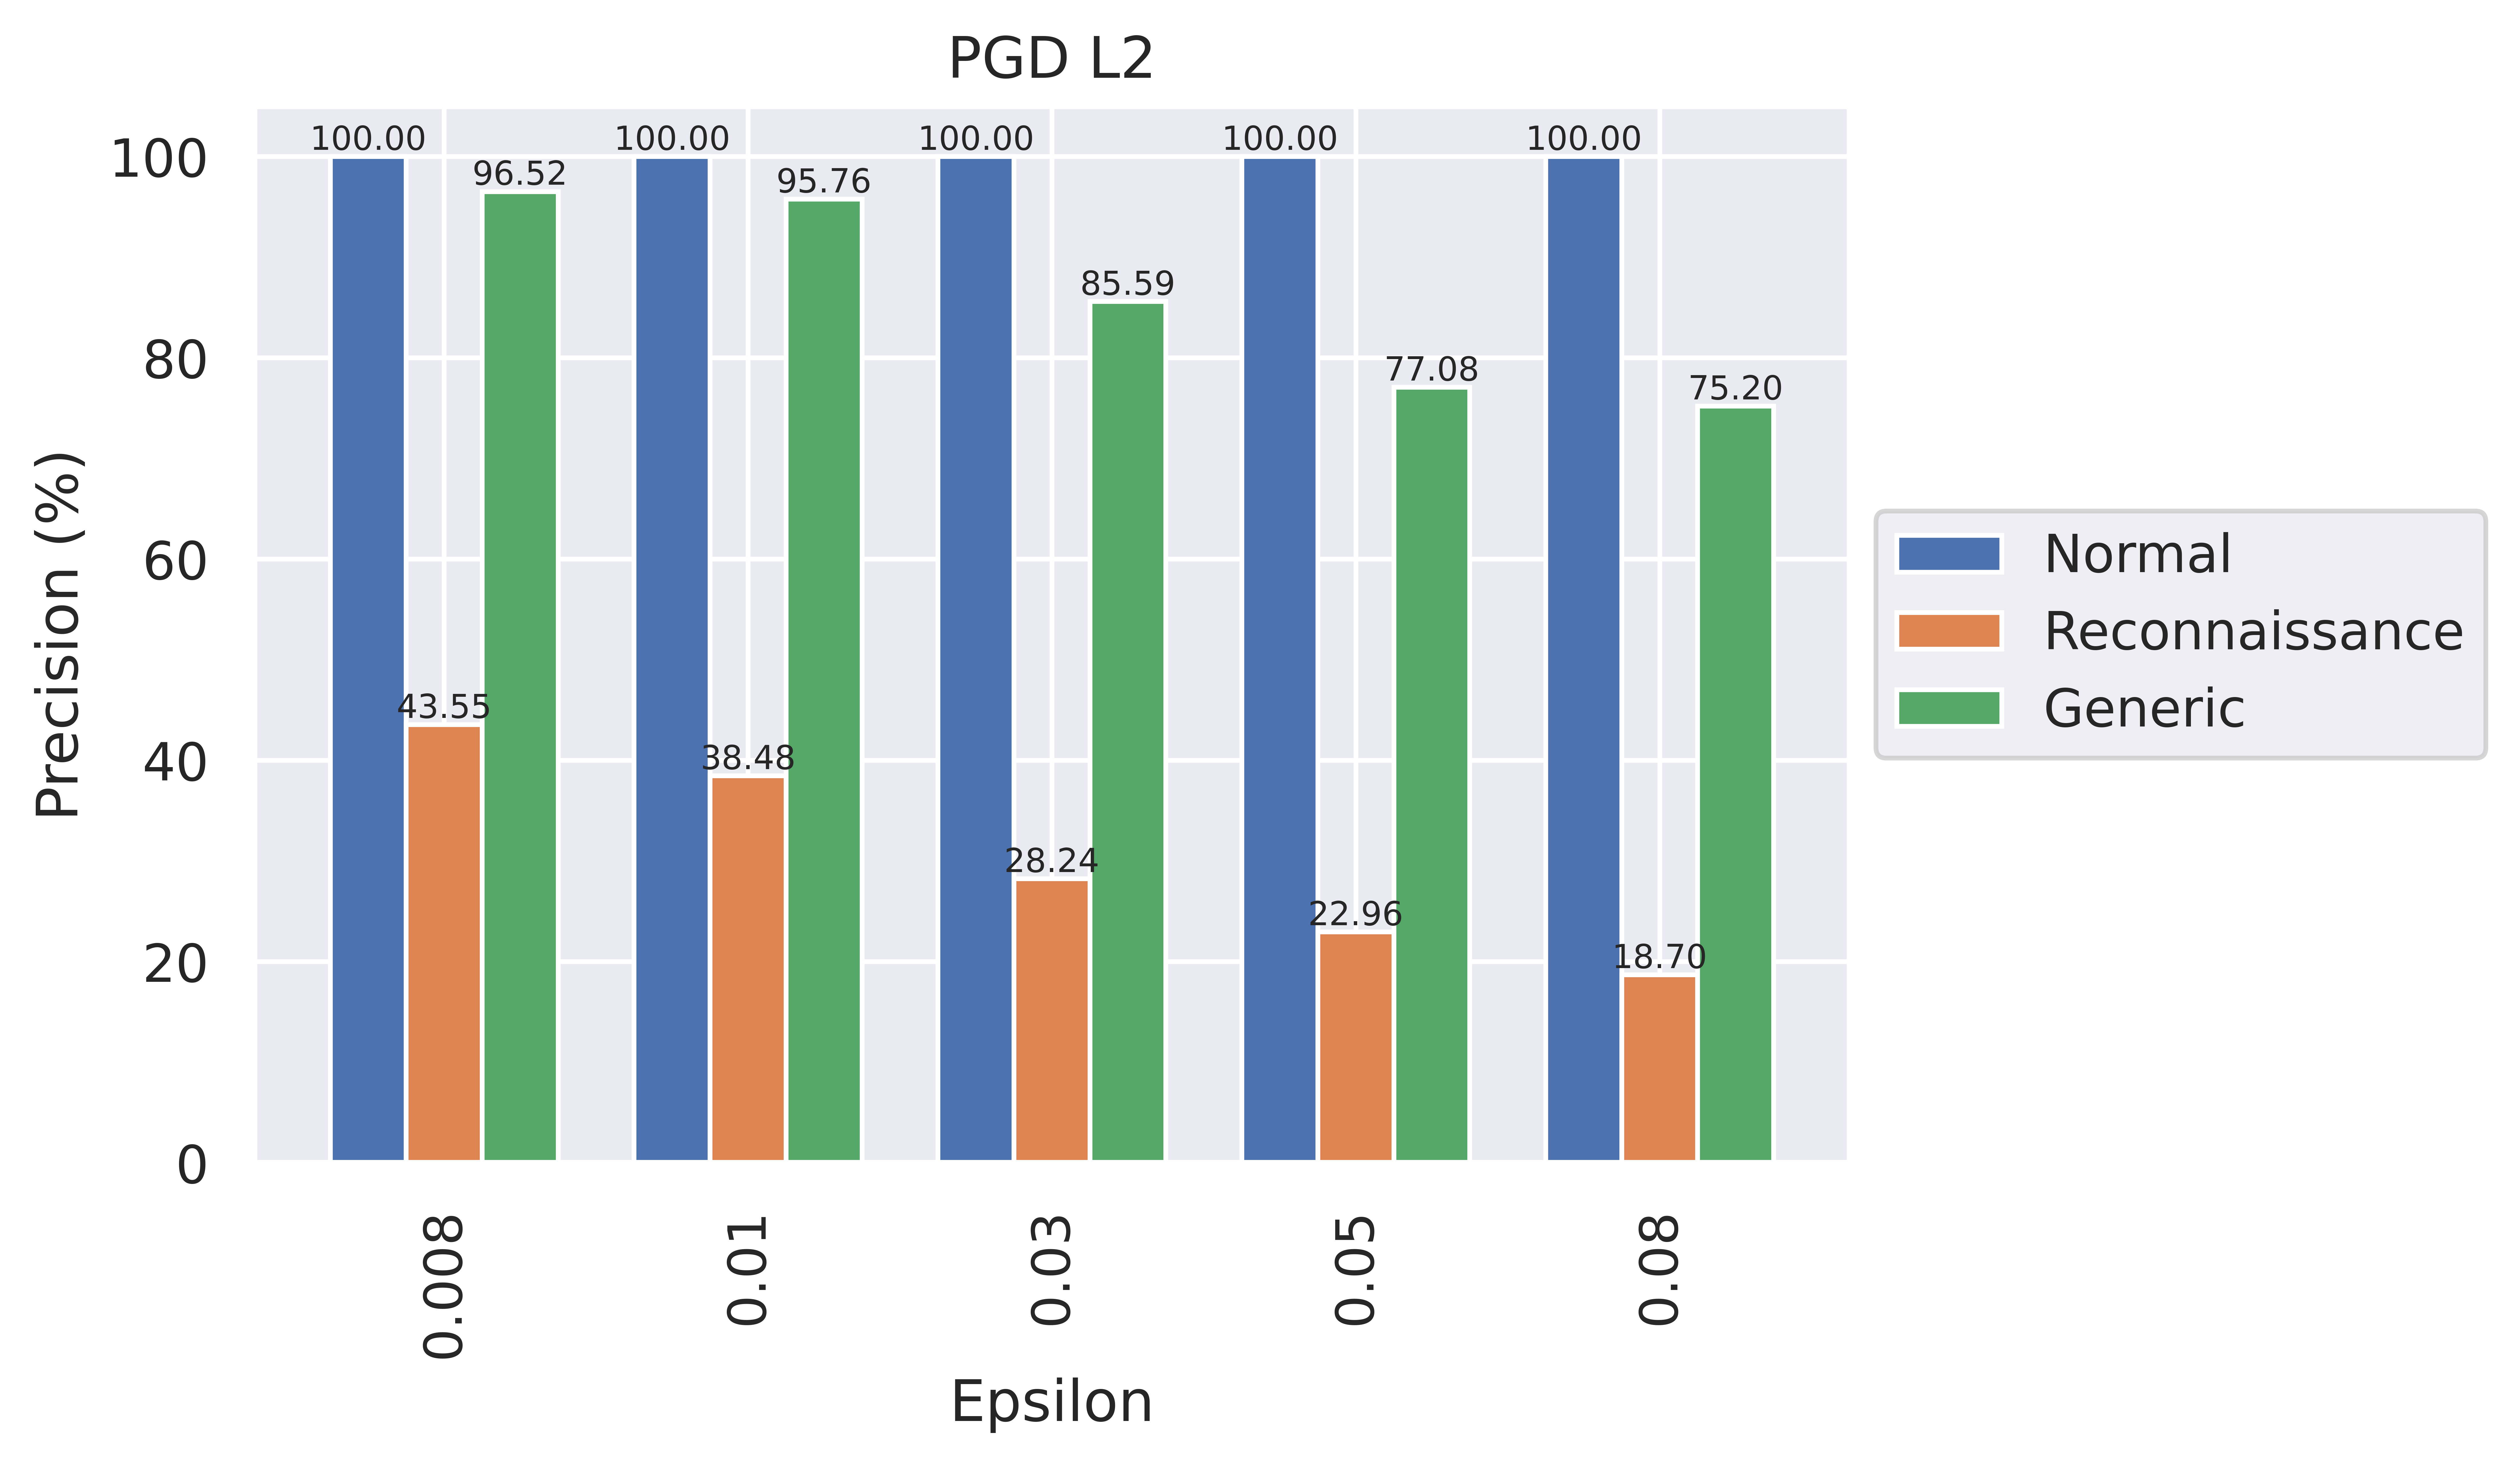
\includegraphics[width=\textwidth]{/home/wojtyla/Documentos/Artigo_2023/IJCNN_Suplementary/Figures//UNSW_IDS_PGD L2_multi_paper.png}
			%caption{Figure}
			\label{fig:5}
		\end{subfigure}
		
		\vskip\baselineskip
		
		\begin{subfigure}[b]{0.45\textwidth}
			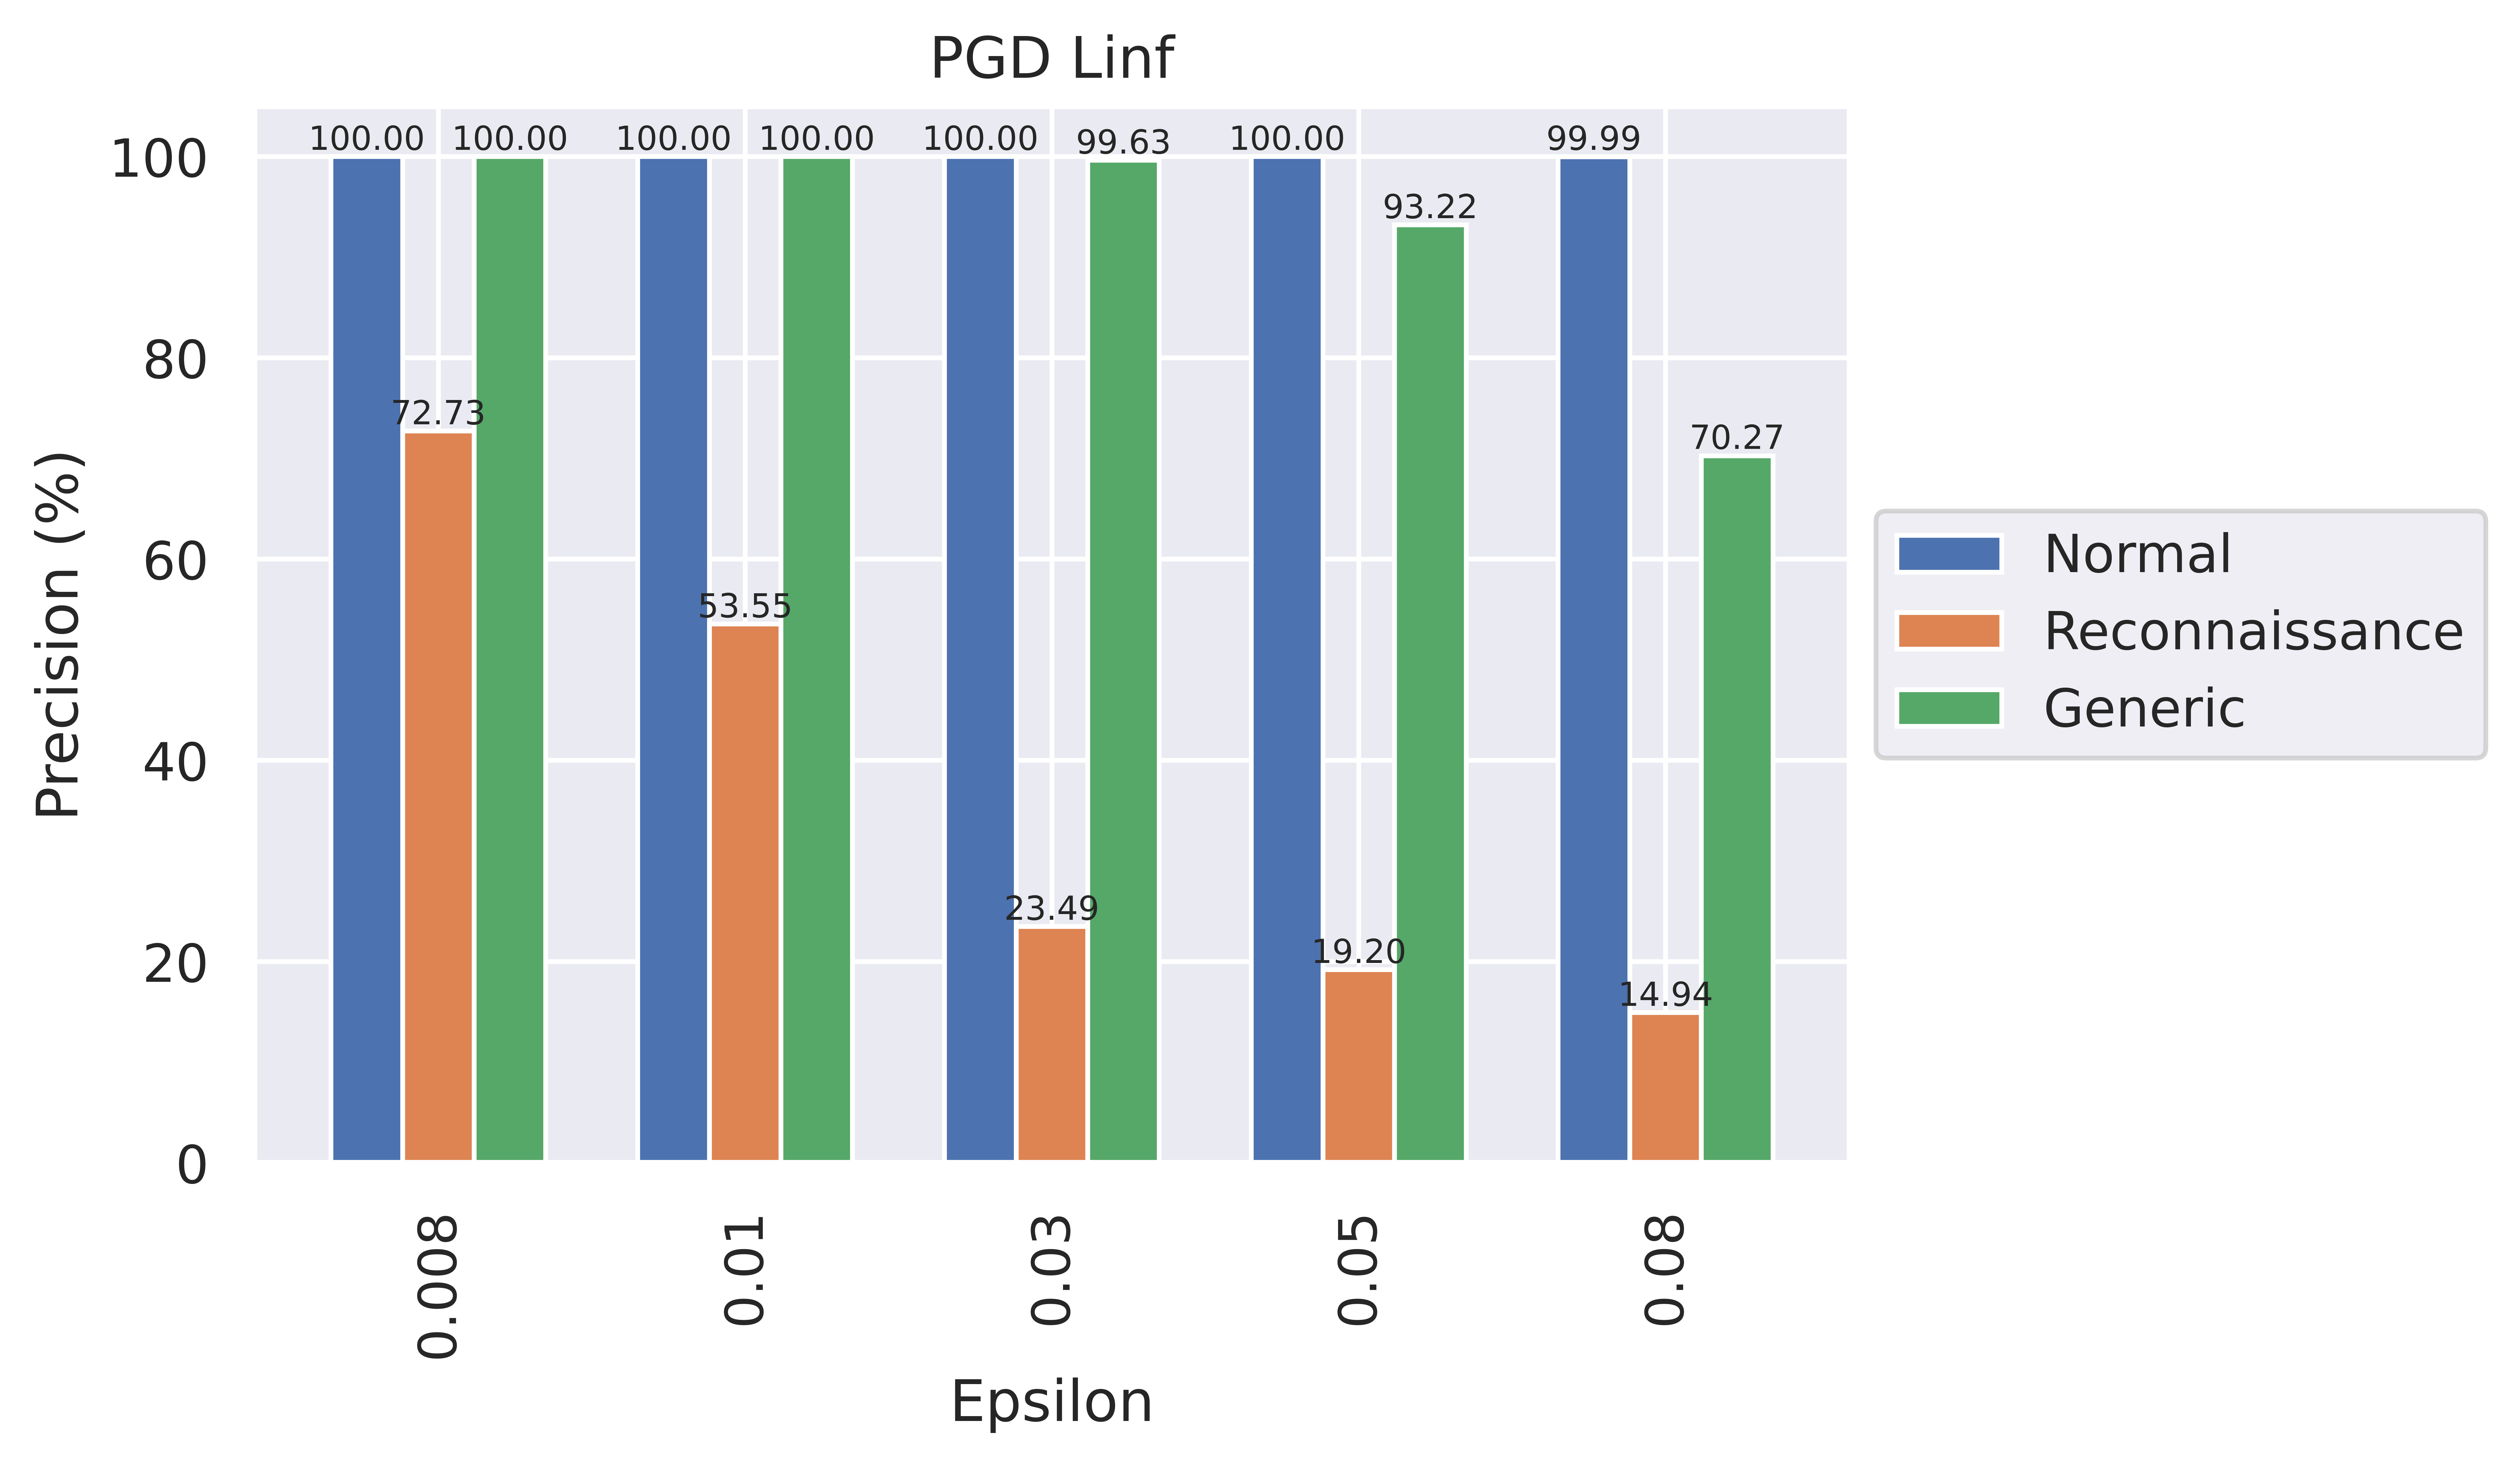
\includegraphics[width=\textwidth]{/home/wojtyla/Documentos/Artigo_2023/IJCNN_Suplementary/Figures/UNSW_Clean_PGD Linf_multi_paper.png}
			%caption{Figure}
			\label{fig:3}
		\end{subfigure}			
		\hfill
		\begin{subfigure}[b]{0.45\textwidth}
			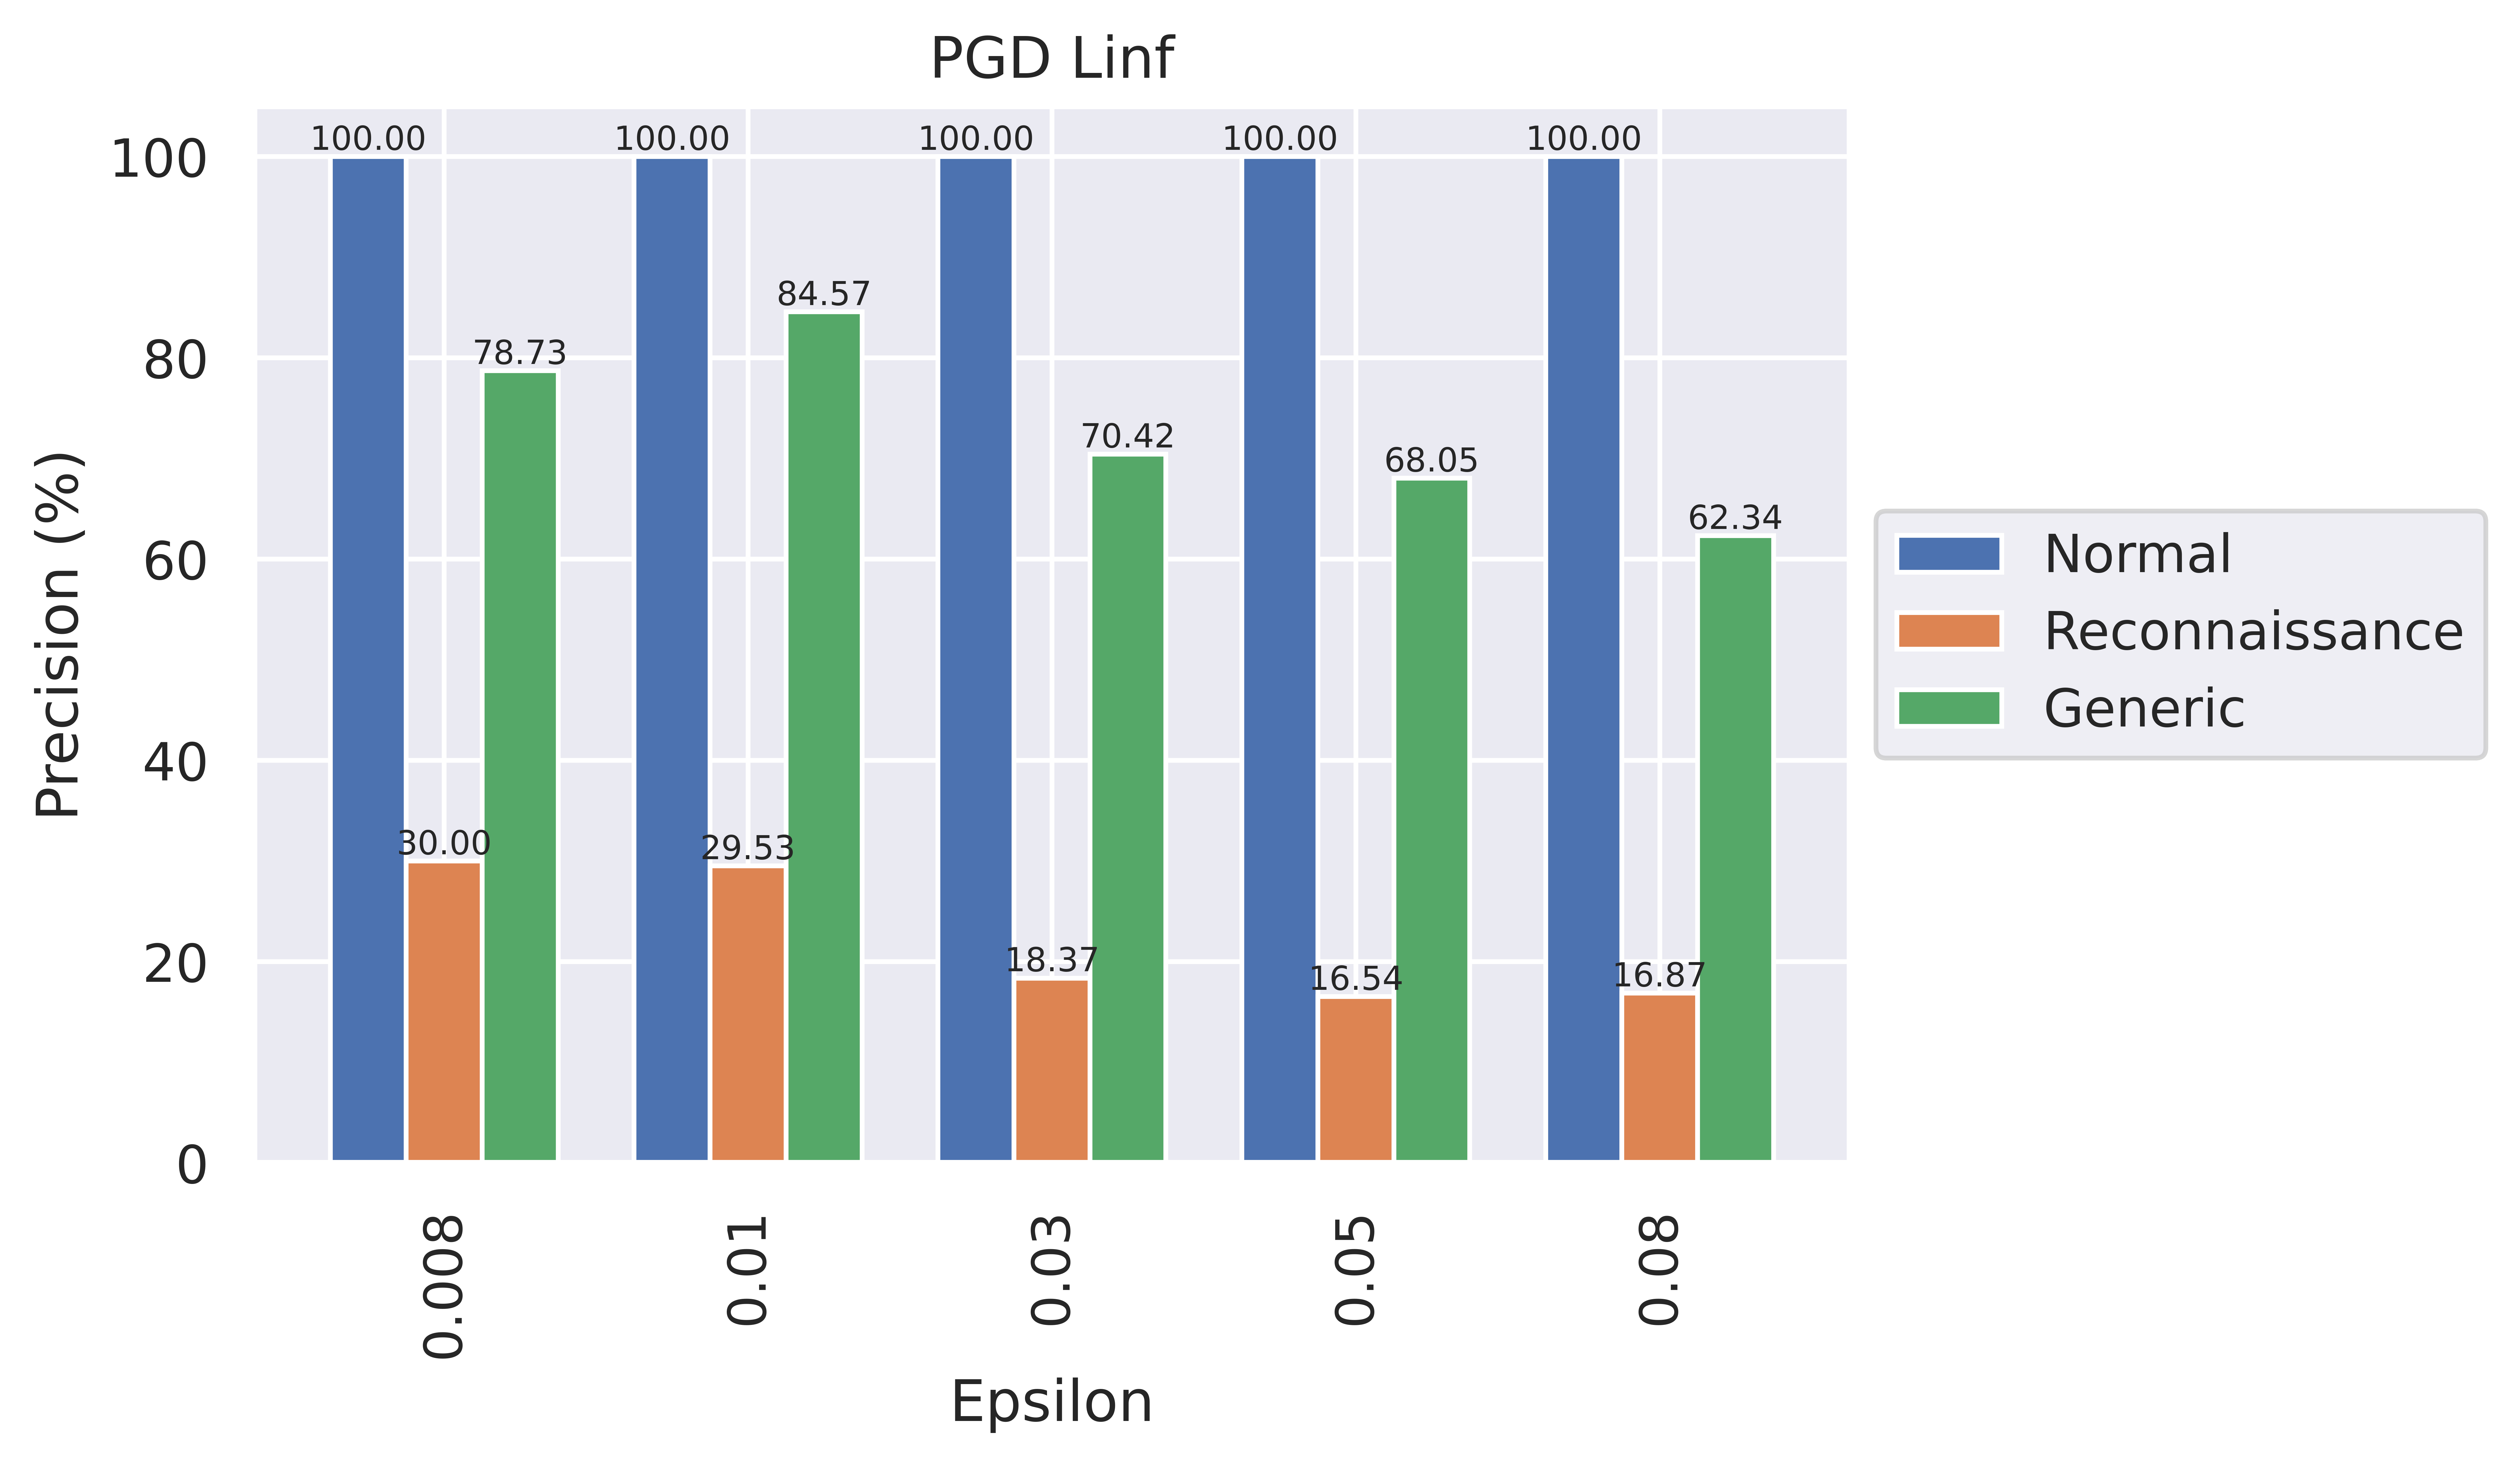
\includegraphics[width=\textwidth]{/home/wojtyla/Documentos/Artigo_2023/IJCNN_Suplementary/Figures//UNSW_IDS_PGD Linf_multi_paper.png}
			%caption{Figure}
			\label{fig:6}
		\end{subfigure}
		\caption{Plots for PGD-100 attack on binary models with UNSW-NB15.Left:EnC model; Right:EnIDS model.}
		\label{fig:unsw_pgd_multi}
	\end{figure}
	
	
	\section{Carlini-Wagner (CW-2)}
	
	\subsection{CIC IDS2017}	
	
	\begin{table}[H]
		\caption{CW-2 attack against EnC and EnIDS for binary classification on the CIC IDS2017 dataset.}
		\small
		\setlength{\tabcolsep}{1pt}
		\centering
		\label{tab:cic_bin_cw}
		%\hspace*{-1cm}
		
		\begin{tabular}{|c|c|c|c|c|c|c|c|c|c|c|c|}
			\hline
			\multirow{4}{*}{\textbf{Type}} & \multirow{4}{*}{\textbf{Metric}}& \multicolumn{10}{c|}{\textbf{Confidence}} \\
			\cline{3-12}
			&  & \multicolumn{2}{c|}{\textbf{0.0}} & \multicolumn{2}{c|}{\textbf{0.2}} & \multicolumn{2}{c|}{\textbf{0.5}} & \multicolumn{2}{c|}{\textbf{0.8}} & \multicolumn{2}{c|}{\textbf{1.0}}  
			\\
			\cline{3-12}
			&  &  \textbf{\textsl{Benign}} & \textbf{\textsl{Attacks}} & \textbf{\textsl{Benign}} & \textbf{\textsl{Attacks}} & \textbf{\textsl{Benign}} & \textbf{\textsl{Attacks}} & \textbf{\textsl{Benign}} & \textbf{\textsl{Attacks}} & \textbf{\textsl{Benign}} & \textbf{\textsl{Attacks}} \\
			\hline
			\multirow{3}{*}{EnC} & Precision & 99.99 & 98.69 & 99.99 & 98.70 & 99.99 & 98.71 & 99.99 & 98.74 & 99.99 & 98.74
			\\
			
			
			& Recall & 99.73 & 99.95 & 99.73 & 99.95 & 99.73 & 99.95 & 99.74 & 99.95 & 99.74 & 99.95
			\\
			
			
			& ROC-AUC & 100.00 & 100.00 & 100.00 & 100.00 & 100.00 & 100.00 & 100.00 & 100.00 & 100.00 & 100.00
			\\
			\hline
			\multirow{3}{*}{EnIDS} & Precision & 99.98 & \cellcolor{yellow!50}99.07 & 99.98 & \cellcolor{yellow!50}99.09 & 99.98 & \cellcolor{yellow!50}99.11 & 99.98 & \cellcolor{yellow!50}99.11 & 99.98 & \cellcolor{yellow!50}99.11
			\\
			
			
			& Recall & \cellcolor{yellow!50}99.81 & 99.89 & \cellcolor{yellow!50}99.81 & 99.89 & \cellcolor{yellow!50}99.82 & 99.89 & \cellcolor{yellow!50}99.82 & 99.89 & \cellcolor{yellow!50}99.82 & 99.89
			\\
			
			
			& ROC-AUC & 99.98 & 99.99 & 99.98 & 99.99 & 99.98 & 99.99 & 99.98 & 99.99 & 99.98 & 99.99
			\\
			\hline
		\end{tabular}
		
	\end{table}
	
	
	\begin{figure}[H]
		\centering
		\begin{subfigure}[b]{0.45\textwidth}
			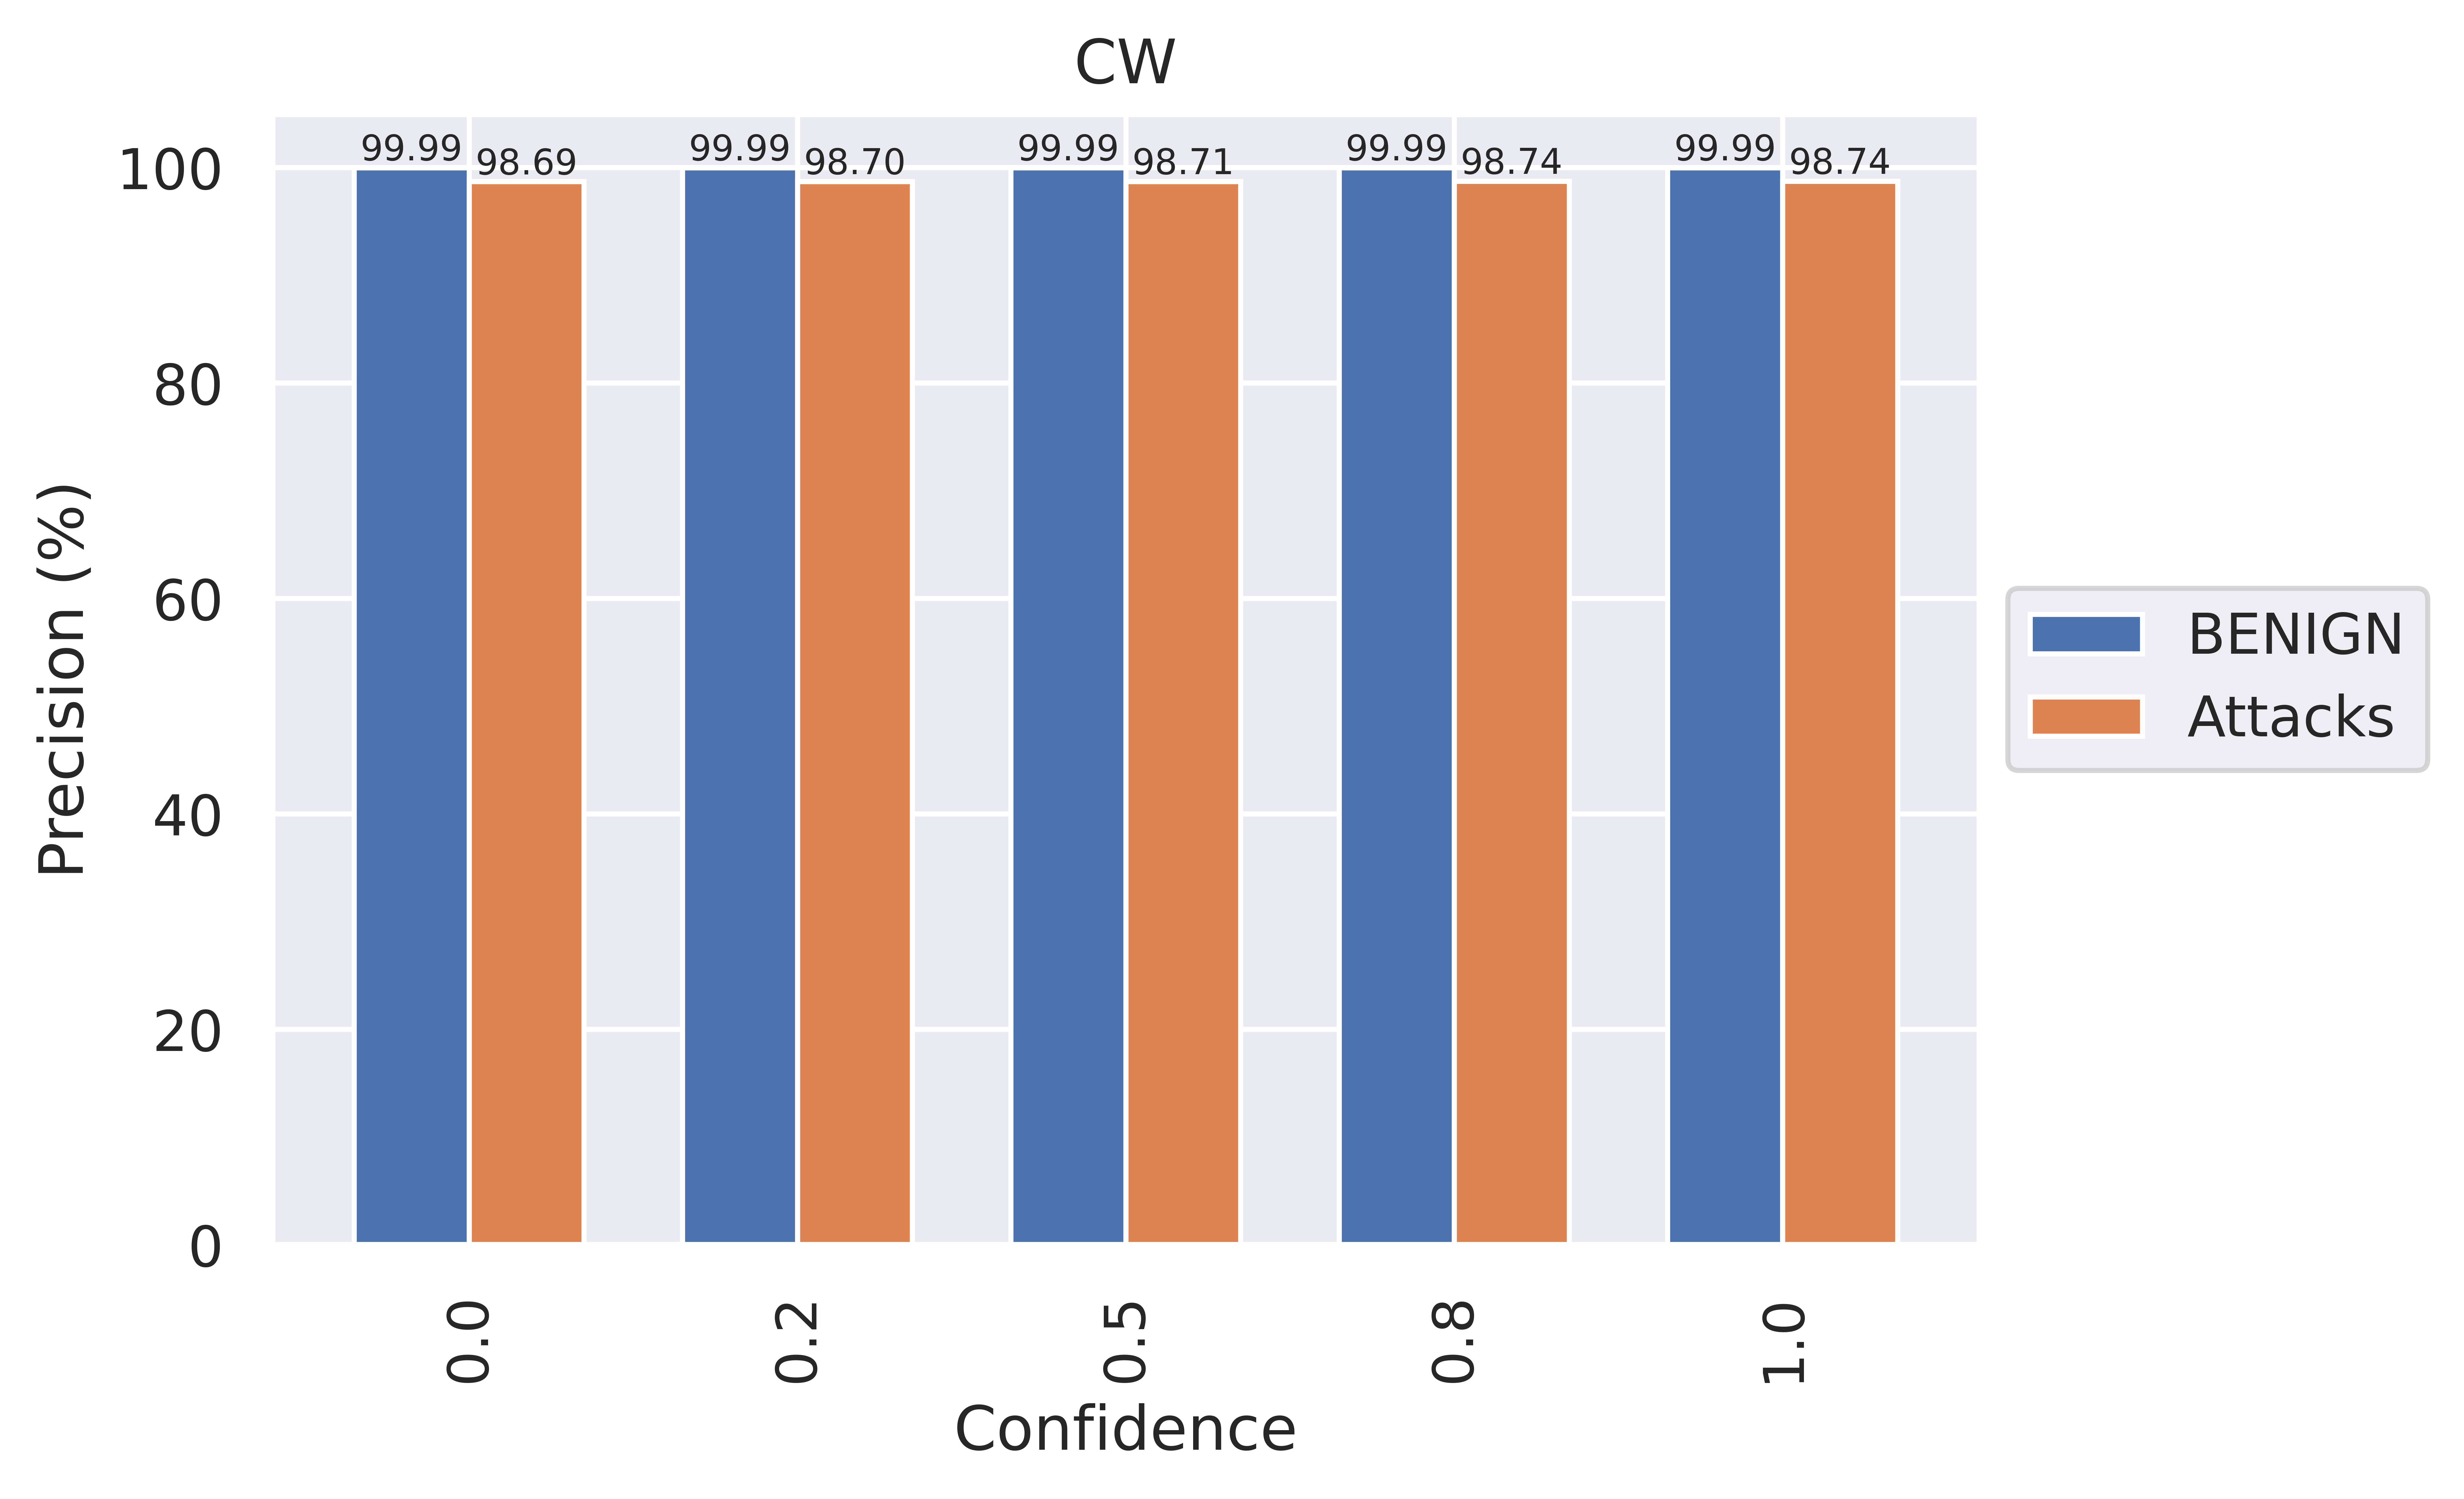
\includegraphics[width=\textwidth]{/home/wojtyla/Documentos/Artigo_2023/IJCNN_Suplementary/Figures//CIC_Clean_CW_bin_paper.png}
			%caption{Figure}
			\label{fig:1}
		\end{subfigure}
		\hfill
		\begin{subfigure}[b]{0.45\textwidth}
			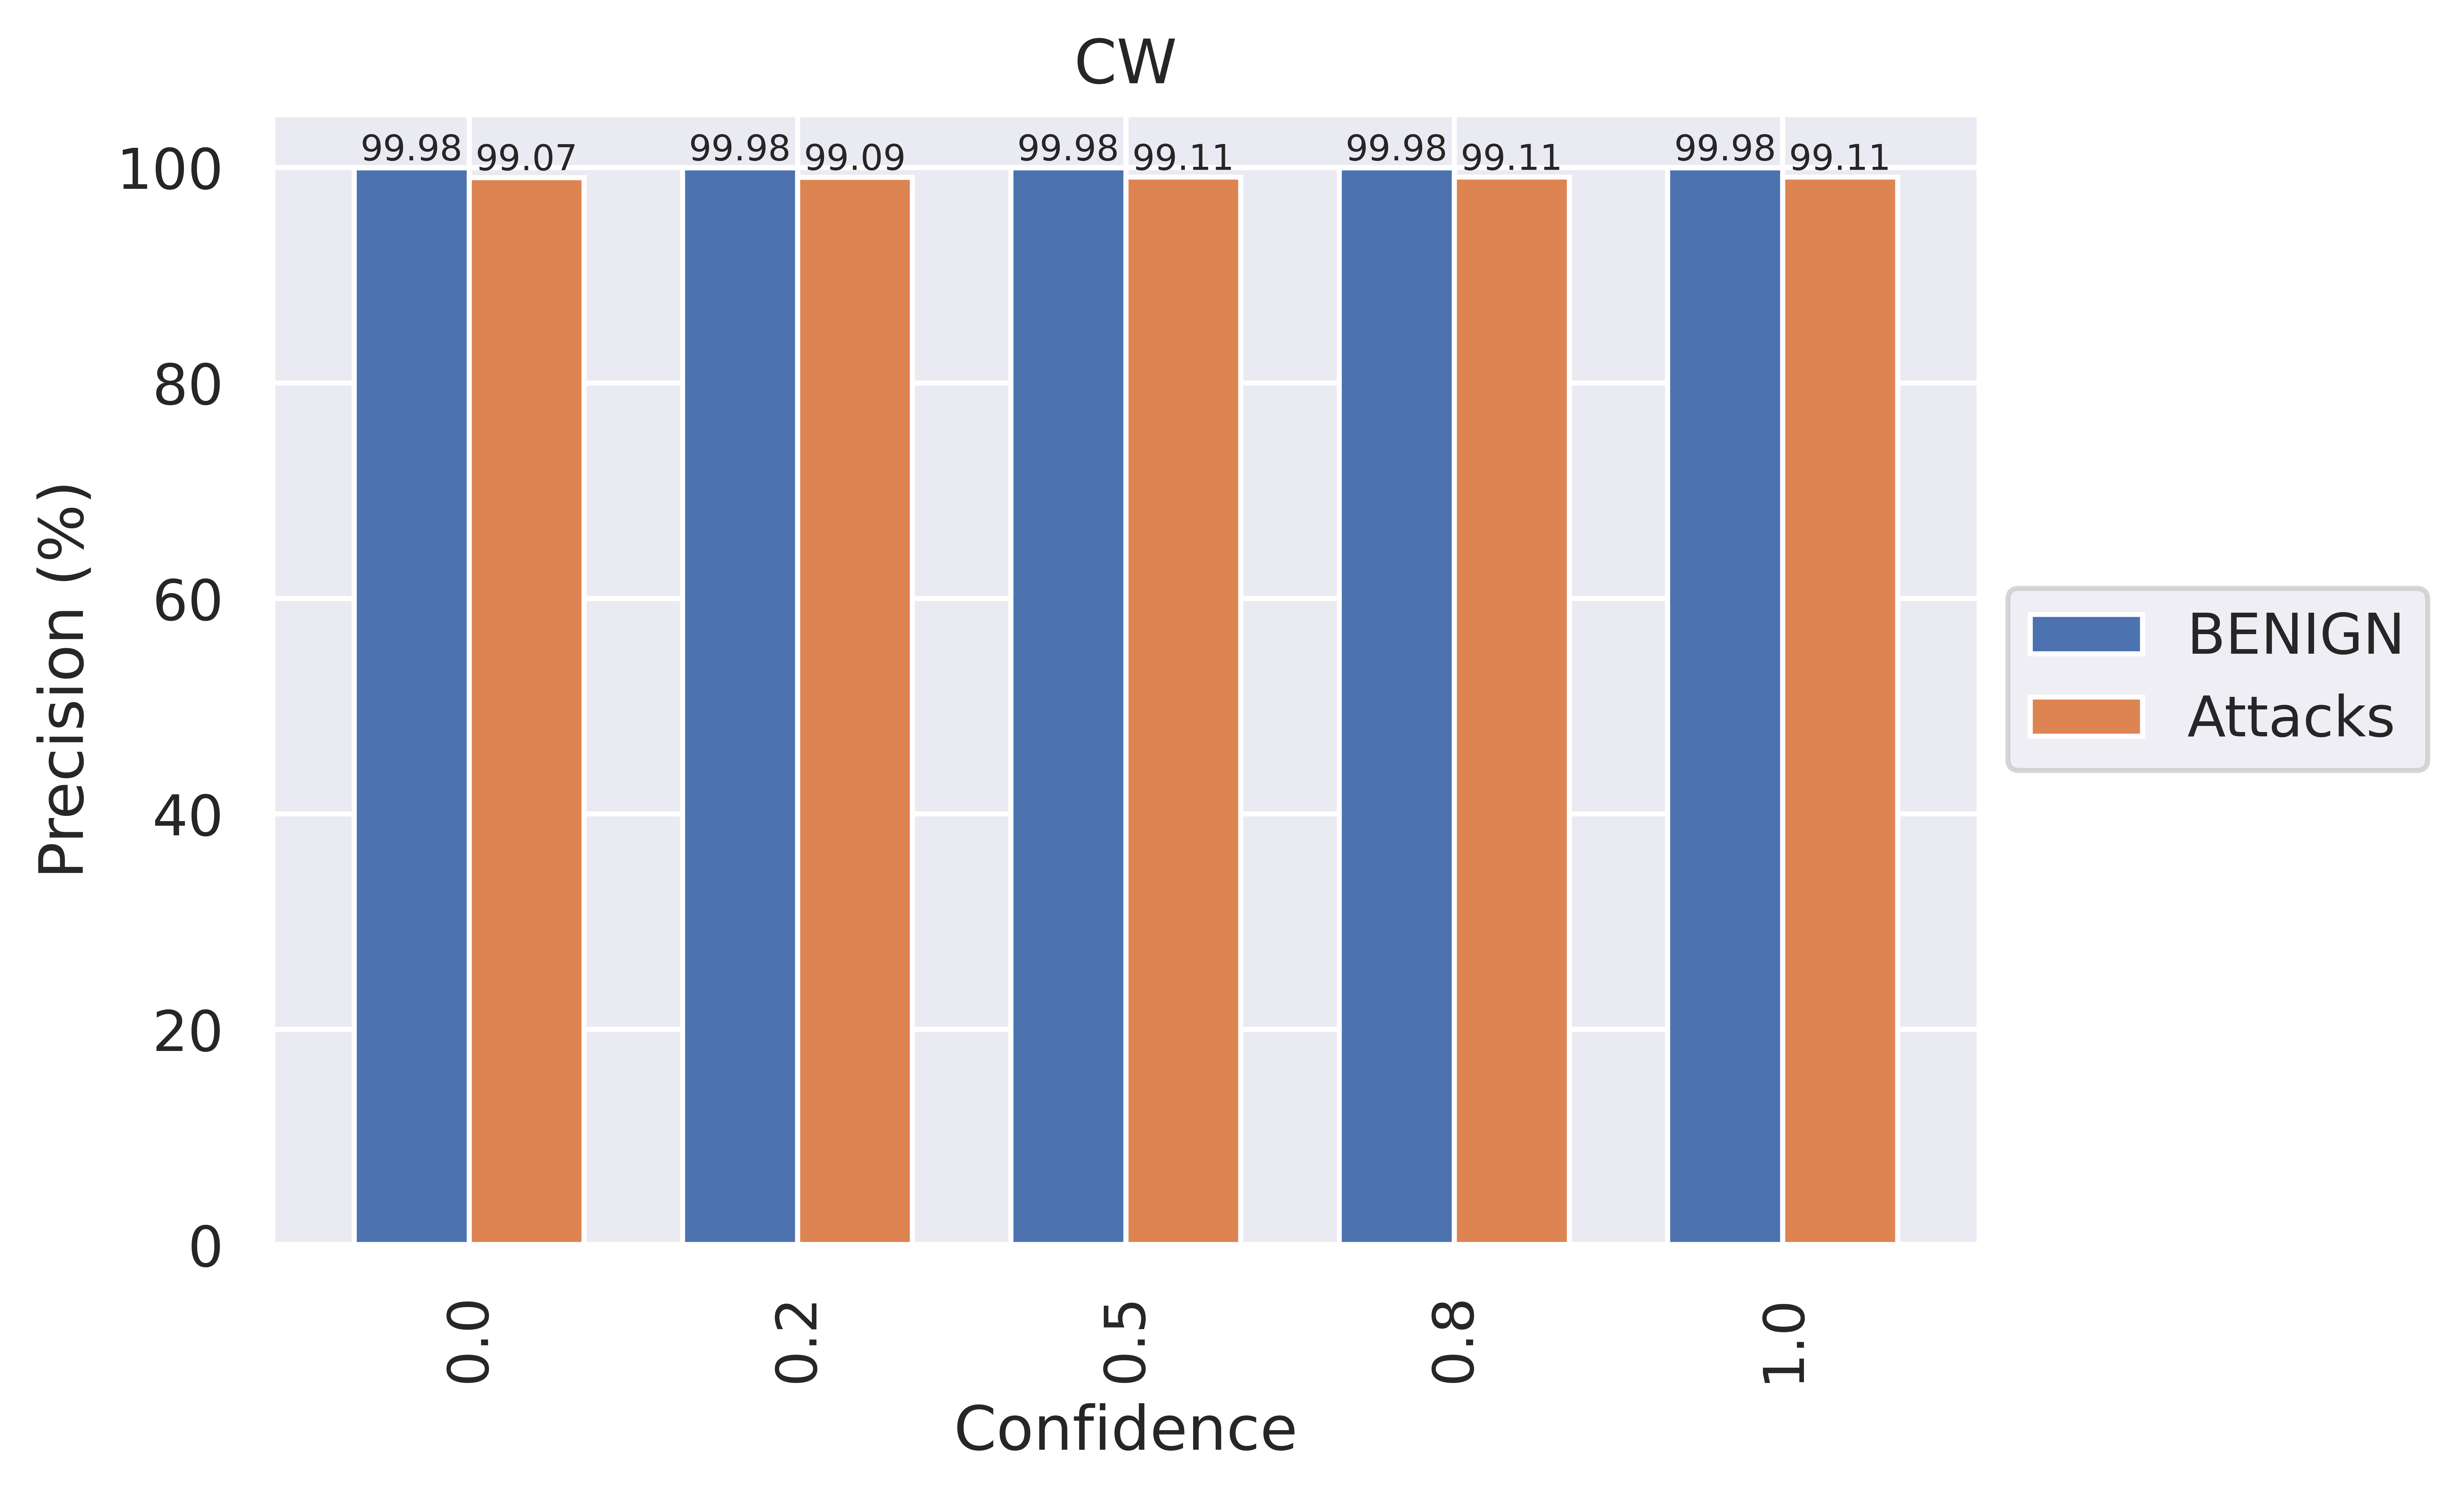
\includegraphics[width=\textwidth]{/home/wojtyla/Documentos/Artigo_2023/IJCNN_Suplementary/Figures//CIC_IDS_CW_bin_paper.png}
			%caption{Figure}
			\label{fig:4}
		\end{subfigure}
		\caption{Plots for CW-2 attack on binary models with CIC IDS2017.Left:EnC model; Right:EnIDS model.}
		\label{fig:cic_cw_bin}
	\end{figure}
	
	
	\begin{table}[H]
		\caption{CW-2 attack against EnC and EnIDS for multiclass classification on the CIC IDS2017 dataset.}
		\small
		\setlength{\tabcolsep}{1pt}
		\centering
		\label{tab:cic_multi_cw}
		\hspace*{-1cm}
		\begin{tabular}{|c|c|c|c|c|c|c|c|c|c|c|c|c|c|c|c|c|}
			\hline
			\multirow{4}{*}{\textbf{Type}} & \multirow{4}{*}{\textbf{Metric}}& \multicolumn{15}{c|}{\textbf{Confidence}} \\
			\cline{3-17}
			&  & \multicolumn{3}{c|}{\textbf{0.0}} & \multicolumn{3}{c|}{\textbf{0.2}} & \multicolumn{3}{c|}{\textbf{0.5}} & \multicolumn{3}{c|}{\textbf{0.8}} & \multicolumn{3}{c|}{\textbf{1.0}} 
			\\
			\cline{3-17}
			&  & \textbf{\textsl{Benign}} & \textbf{\textsl{DoS}} & \textbf{\textsl{DDoS}} & \textbf{\textsl{Benign}} & \textbf{\textsl{DoS}} & \textbf{\textsl{DDoS}} & \textbf{\textsl{Benign}} & \textbf{\textsl{DoS}} & \textbf{\textsl{DDoS}} & \textbf{\textsl{Benign}} & \textbf{\textsl{DoS}} & \textbf{\textsl{DDoS}} & \textbf{\textsl{Benign}} & \textbf{\textsl{DoS}} & \textbf{\textsl{DDoS}}
			\\
			\hline
			\multirow{3}{*}{EnC} & Precision & 99.99 & 99.23 & 99.99 & 99.99 & 99.25 & 99.99 & 99.99 & 99.26 & 99.99 & 99.99 & 99.28 & 99.99 & 99.99 & 99.29 & 99.99
			\\
			
			& Recall & 99.36 & 99.75 & 99.99 & 99.38 & 99.75 & 99.99 & 99.39 & 99.75 & 99.99 & 99.41 & 99.75 & 99.99 & 99.42 & 99.76 & 99.99
			\\
			
			& ROC-AUC & 99.98 & 100.00 & 100.00 & 99.98 & 100.00 & 100.00 & 99.98 & 100.00 & 100.00 & 99.98 & 100.00 & 100.00 & 99.98 & 100.00 & 100.00
			\\
			\hline
			\multirow{3}{*}{EnIDS} & Precision & \cellcolor{blue!20}99.99 & 98.92 & 99.94 & \cellcolor{blue!20}99.99 & 98.93 & 99.94 & \cellcolor{blue!20}99.99 & 98.95 & 99.94 & \cellcolor{blue!20}99.99 & 98.96 & 99.94 & \cellcolor{blue!20}99.99 & 98.97 & 99.94
			\\
			
			& Recall & 97.79 & \cellcolor{yellow!50}99.93 & \cellcolor{yellow!50}100.00 & 97.85 & \cellcolor{yellow!50}99.93 & \cellcolor{yellow!50}100.00 & 97.86 & \cellcolor{yellow!50}99.93 & \cellcolor{yellow!50}100.00 & 97.87 & \cellcolor{yellow!50}99.93 & \cellcolor{yellow!50}100.00 & 97.88 & \cellcolor{yellow!50}99.93 & \cellcolor{yellow!50}100.00
			\\
			
			& ROC-AUC & 99.97 & \cellcolor{blue!20}100.00 & \cellcolor{blue!20}100.00 & 99.97 & \cellcolor{blue!20}100.00 & \cellcolor{blue!20}100.00 & 99.97 & \cellcolor{blue!20}100.00 & \cellcolor{blue!20}100.00 & 99.97 & \cellcolor{blue!20}100.00 & \cellcolor{blue!20}100.00 & 99.97 & \cellcolor{blue!20}100.00 & \cellcolor{blue!20}100.00
			\\
			\hline
		\end{tabular}
		
	\end{table}
	
	\begin{figure}[H]
		\centering
		\begin{subfigure}[b]{0.45\textwidth}
			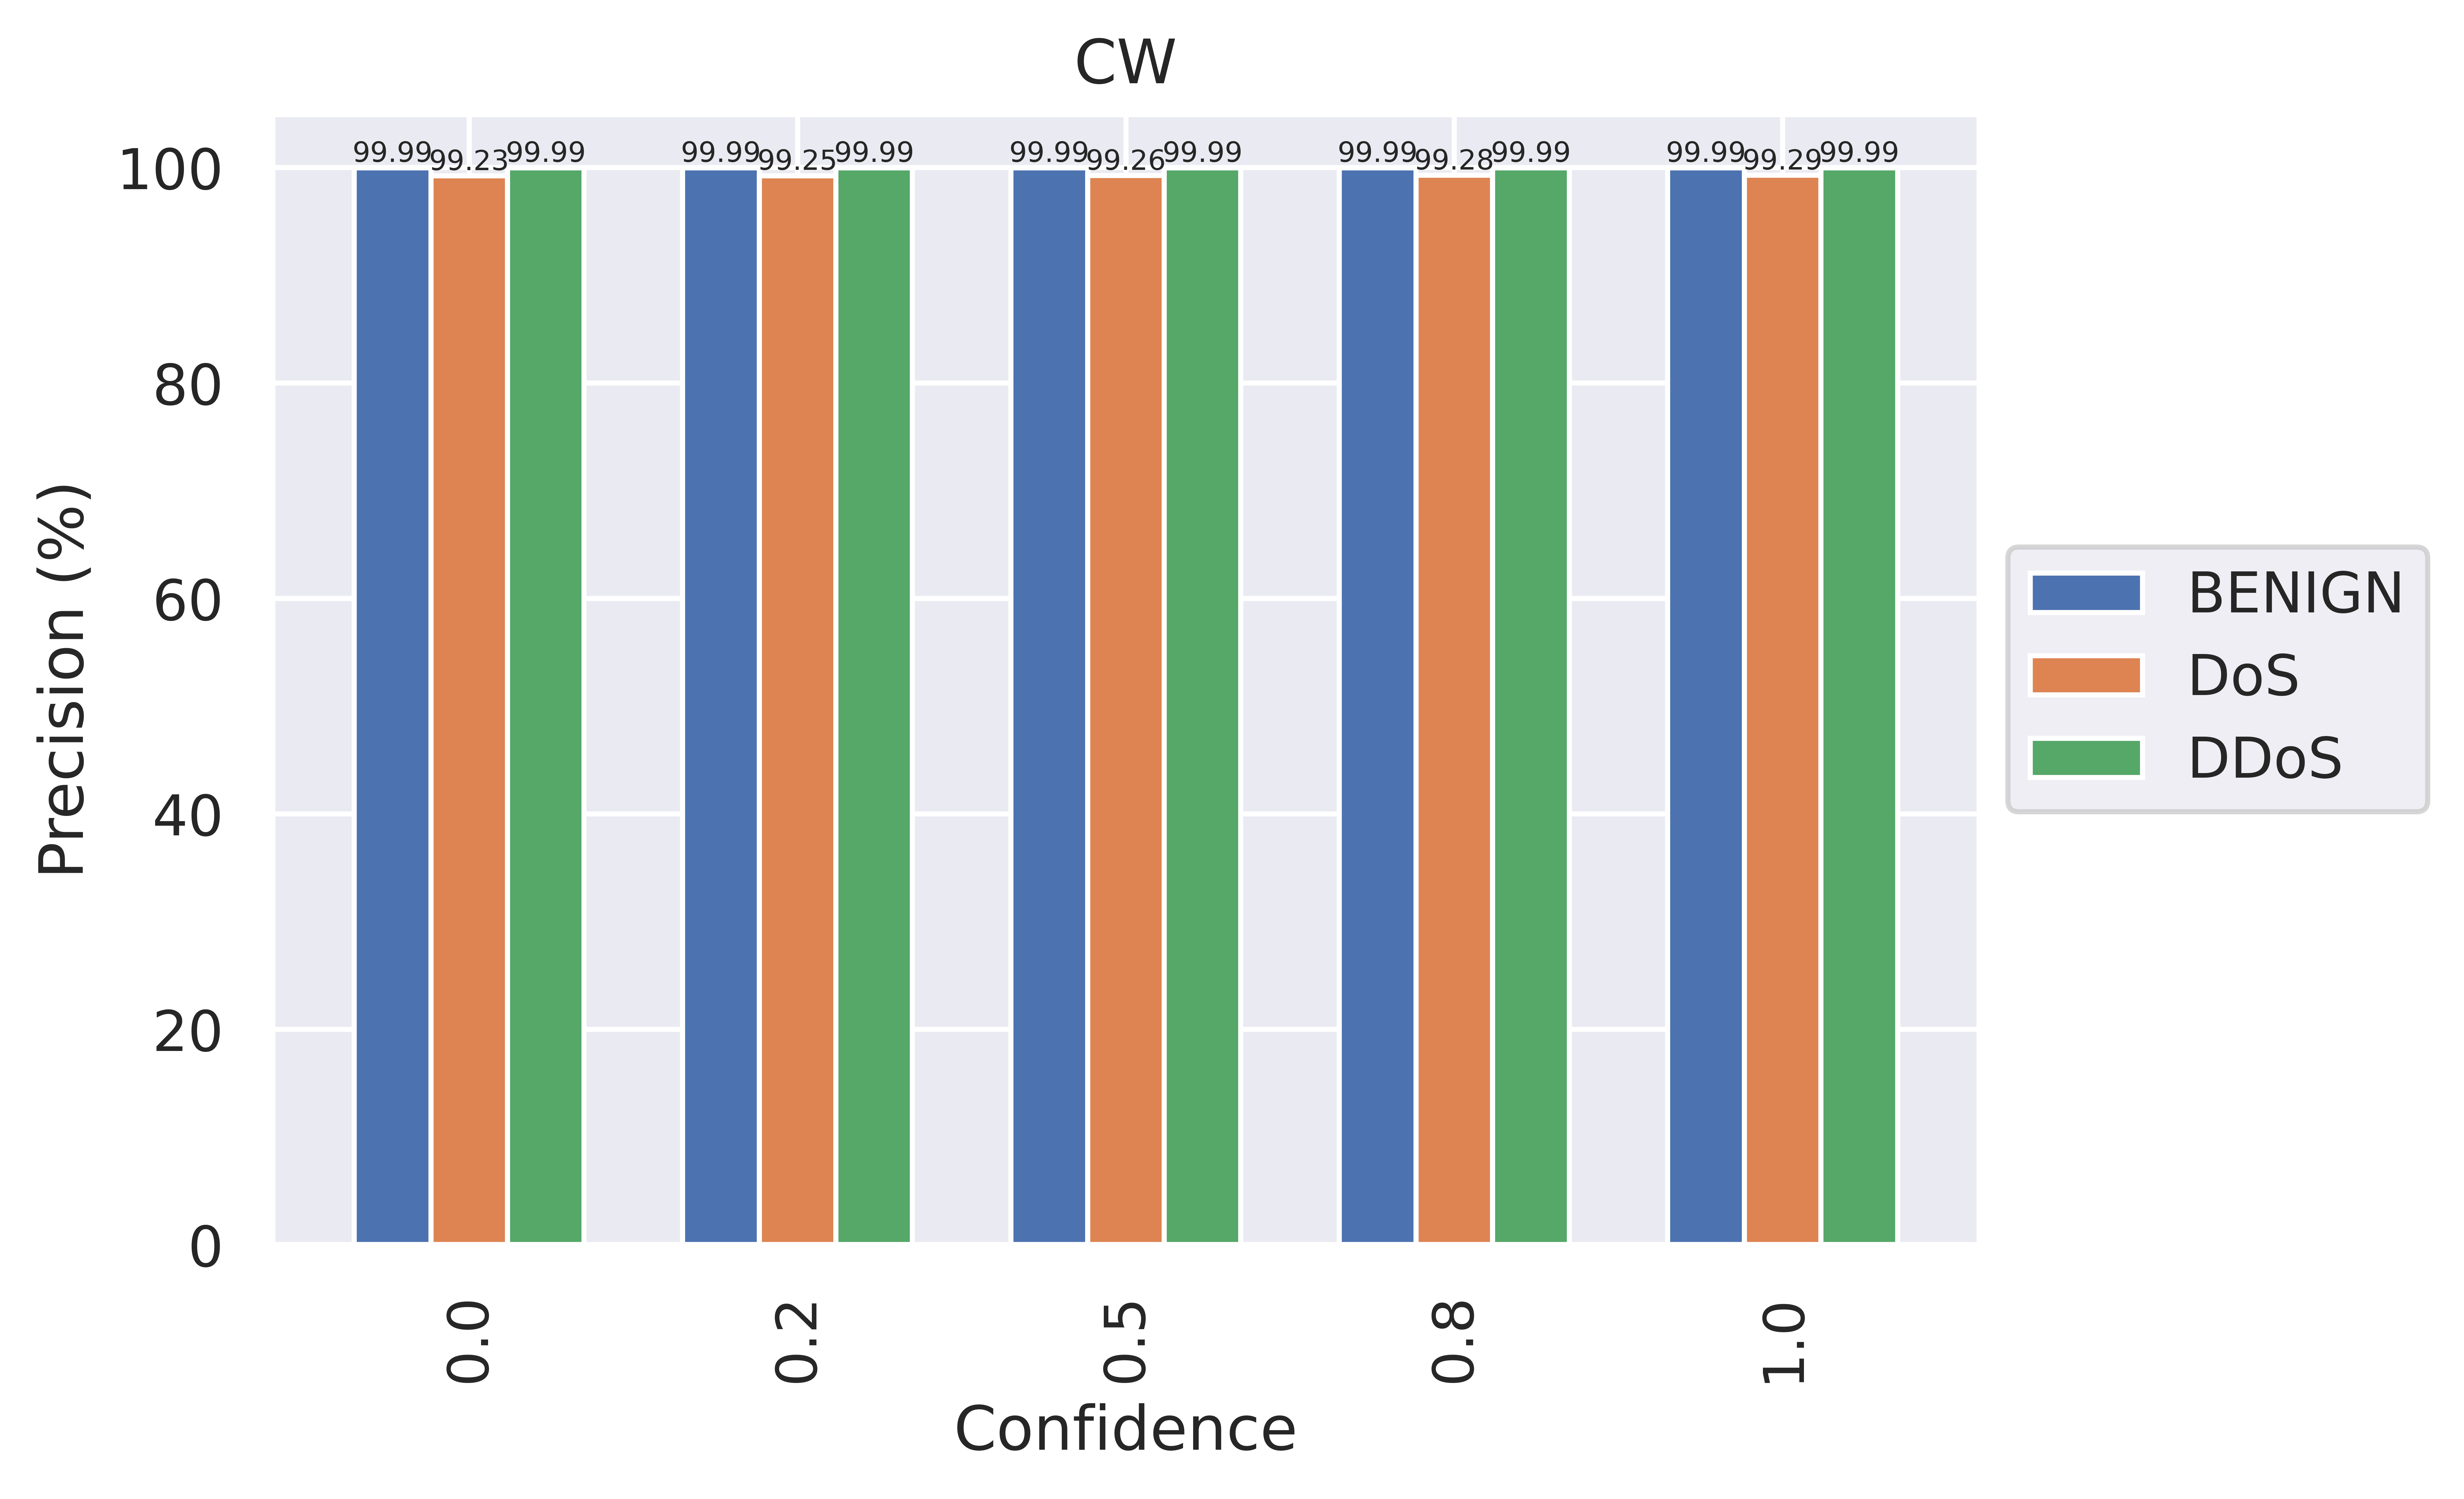
\includegraphics[width=\textwidth]{/home/wojtyla/Documentos/Artigo_2023/IJCNN_Suplementary/Figures//CIC_Clean_CW_multi_paper.png}
			%caption{Figure}
			\label{fig:1}
		\end{subfigure}
		\hfill
		\begin{subfigure}[b]{0.45\textwidth}
			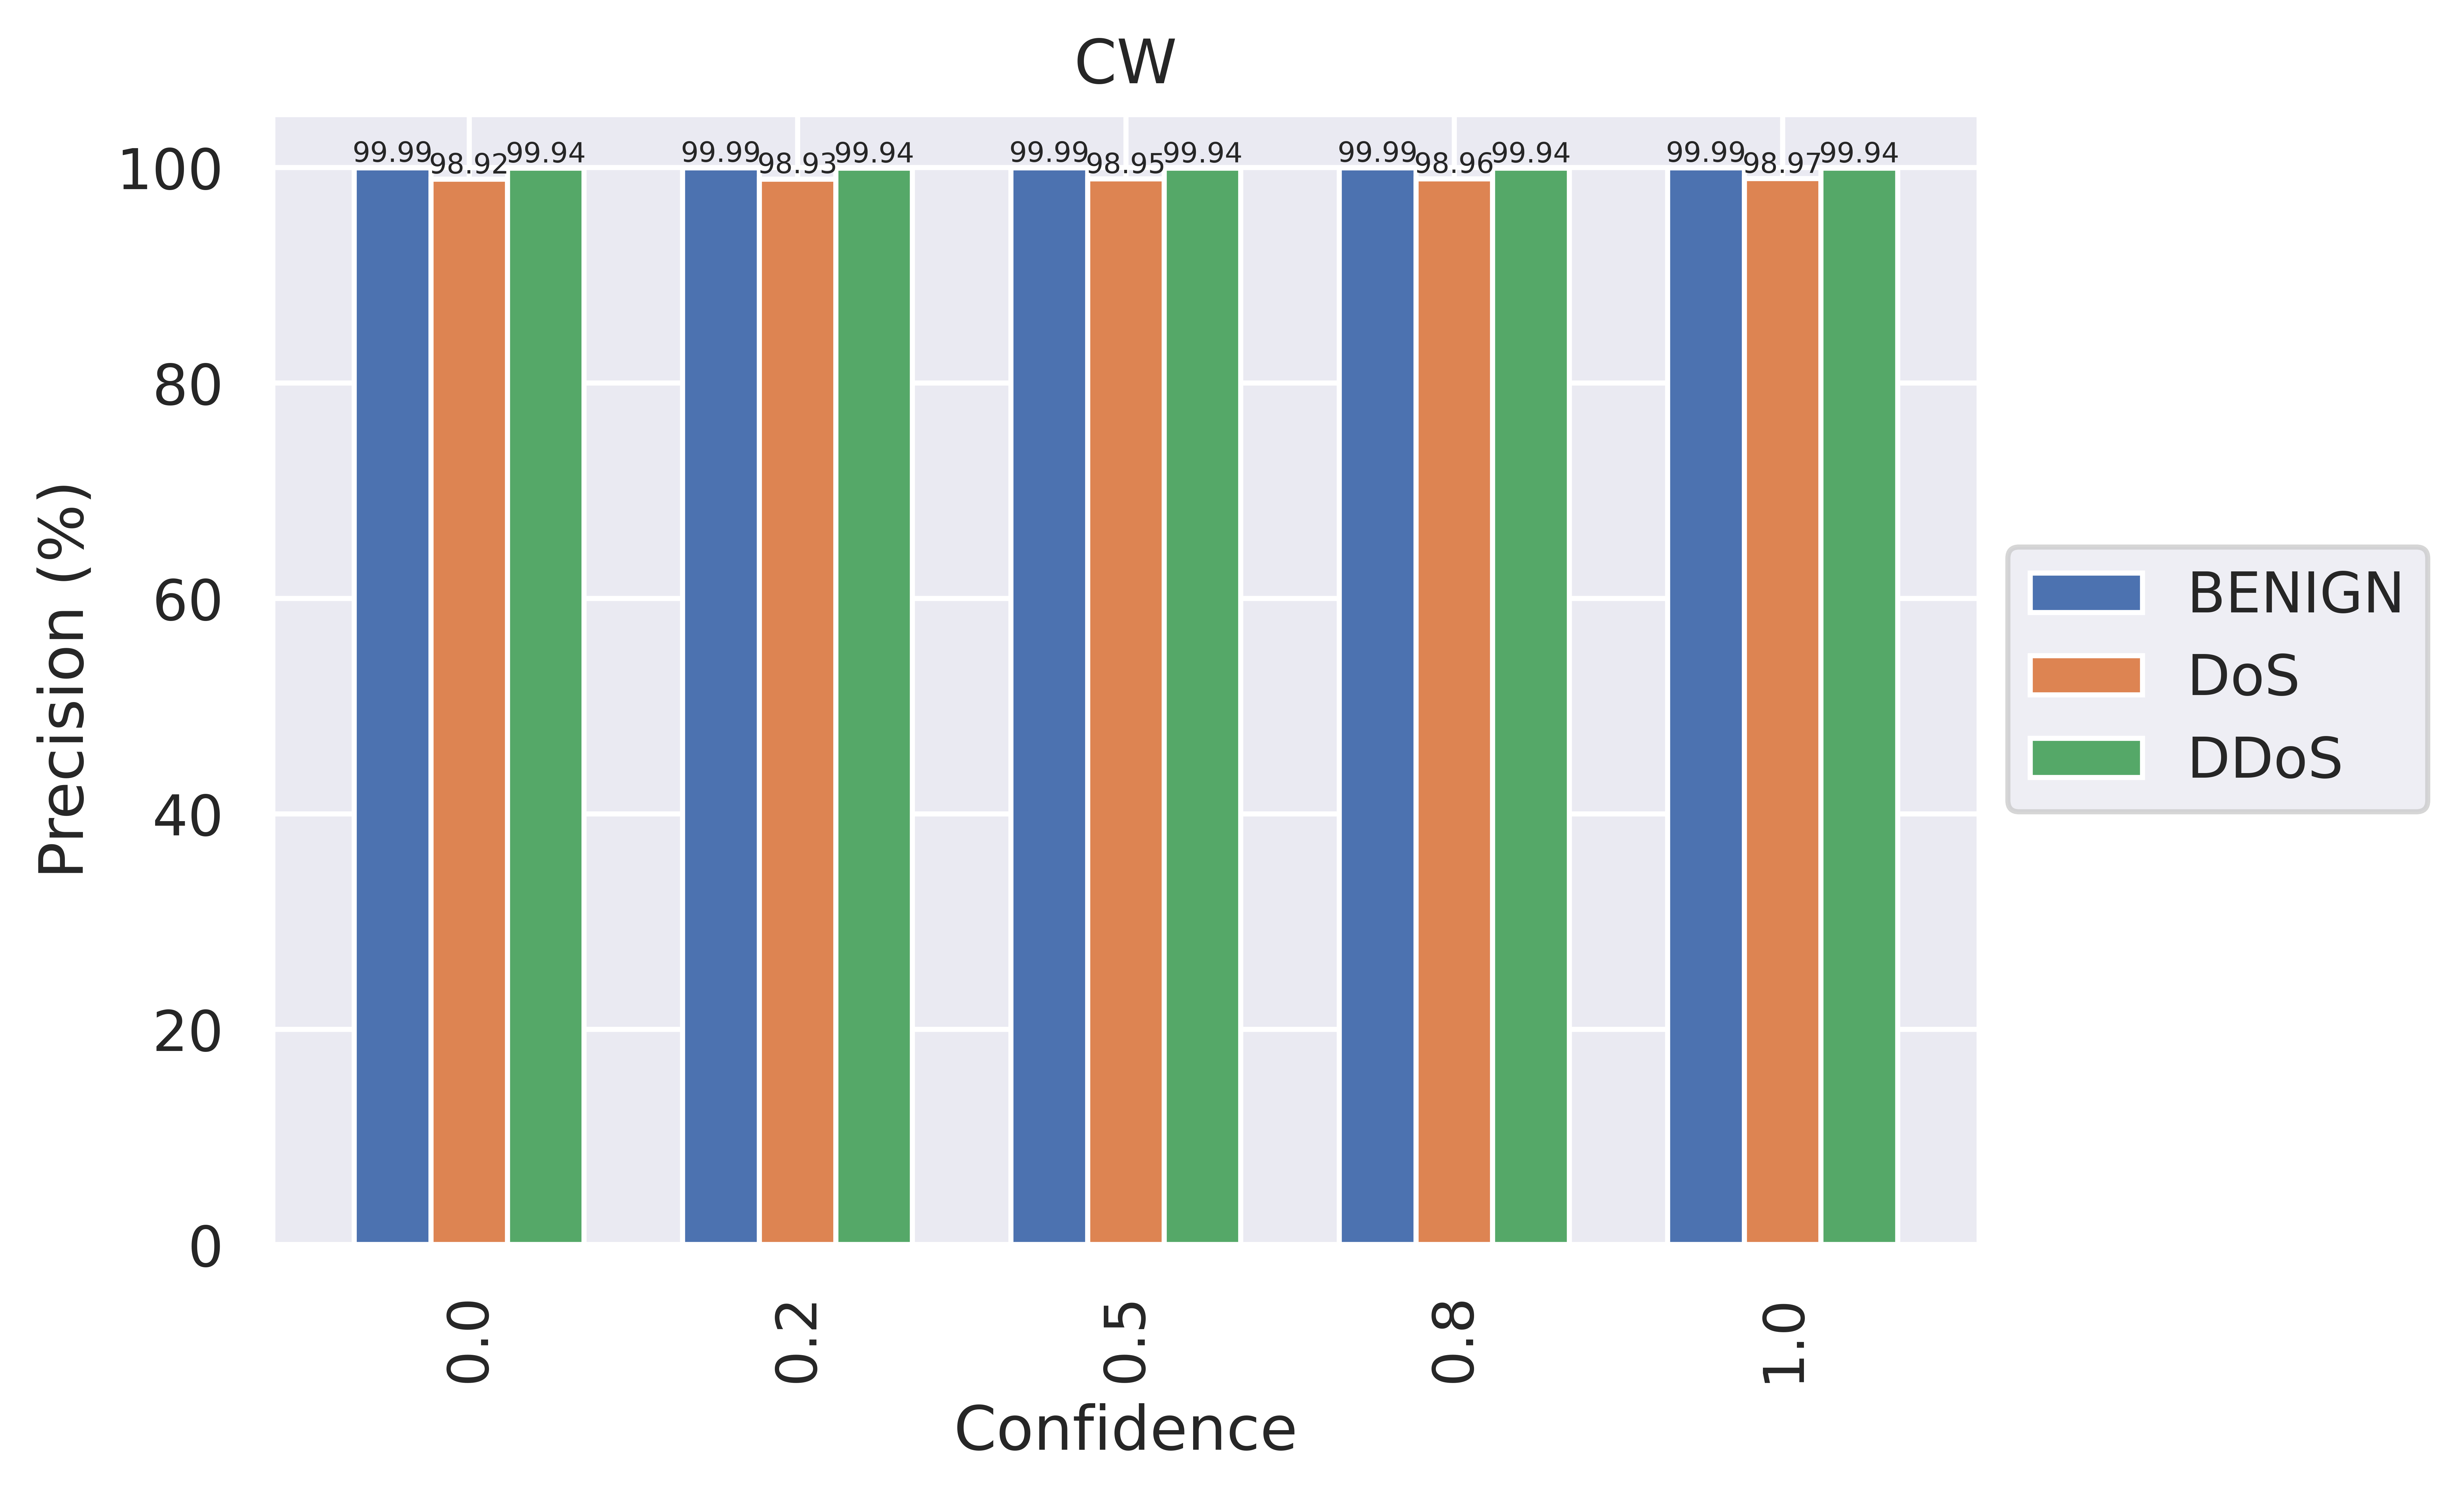
\includegraphics[width=\textwidth]{/home/wojtyla/Documentos/Artigo_2023/IJCNN_Suplementary/Figures//CIC_IDS_CW_multi_paper.png}
			%caption{Figure}
			\label{fig:4}
		\end{subfigure}
		\caption{Plots for CW-2 attack on binary models with CIC IDS2017.Left:EnC model; Right:EnIDS model.}
		\label{fig:cic_cw_multi}
	\end{figure}
	
	
	
	\subsection{UNSW-NB15}
	
	
	\begin{table}[H]
		\caption{CW-2 attack against EnC and EnIDS for binary classification on the UNSW-NB15 dataset.}
		\small
		\setlength{\tabcolsep}{1pt}
		\centering
		\label{tab:unsw_bin_cw}		
		\begin{tabular}{|c|c|c|c|c|c|c|c|c|c|c|c|}
			\hline
			\multirow{4}{*}{\textbf{Type}} & \multirow{4}{*}{\textbf{Metric}}& \multicolumn{10}{c|}{\textbf{Confidence}} \\
			\cline{3-12}
			&  & \multicolumn{2}{c|}{\textbf{0.0}} & \multicolumn{2}{c|}{\textbf{0.2}} & \multicolumn{2}{c|}{\textbf{0.5}} & \multicolumn{2}{c|}{\textbf{0.8}} & \multicolumn{2}{c|}{\textbf{1.0}}   \\
			\cline{3-12}
			&  &  \textbf{\textsl{Normal}} & \textbf{\textsl{Attacks}} & \textbf{\textsl{Normal}} & \textbf{\textsl{Attacks}} & \textbf{\textsl{Normal}} & \textbf{\textsl{Attacks}} & \textbf{\textsl{Normal}} & \textbf{\textsl{Attacks}} & \textbf{\textsl{Normal}} & \textbf{\textsl{Attacks}} \\
			\hline
			\multirow{3}{*}{EnC} & Precision & 100.00 & 84.07 & 100.00 & 84.15 & 100.00 & 84.31 & 100.00 & 84.40 & 100.00 & 84.51
			\\
			
			& Recall & 99.61 & 99.86 & 99.61 & 99.86 & 99.61 & 99.86 & 99.62 & 99.89 & 99.62 & 99.93
			\\
			
			& ROC-AUC & 99.98 & 99.98 & 99.98 & 99.98 & 99.98 & 99.98 & 99.98 & 99.98 & 99.98 & 99.98
			\\
			\hline
			\multirow{3}{*}{EnIDS} & Precision & 99.87 & 4.99 & 99.88 & 5.12 & 99.89 & 5.33 & 99.90 & 5.57 & 99.90 & 5.73
			\\
			
			& Recall & 61.85 & 96.11 & 62.81 & 96.26 & 64.20 & 96.71 & 65.79 & 96.69 & 66.82 & 96.76
			\\
			
			& ROC-AUC & 98.41 & 98.41 & 98.49 & 98.49 & 98.68 & 98.68 & 98.70 & 98.70 & 98.75 & 98.75
			\\
			\hline
		\end{tabular}		
	\end{table}
	
	\begin{figure}[H]
		\centering
		\begin{subfigure}[b]{0.45\textwidth}
			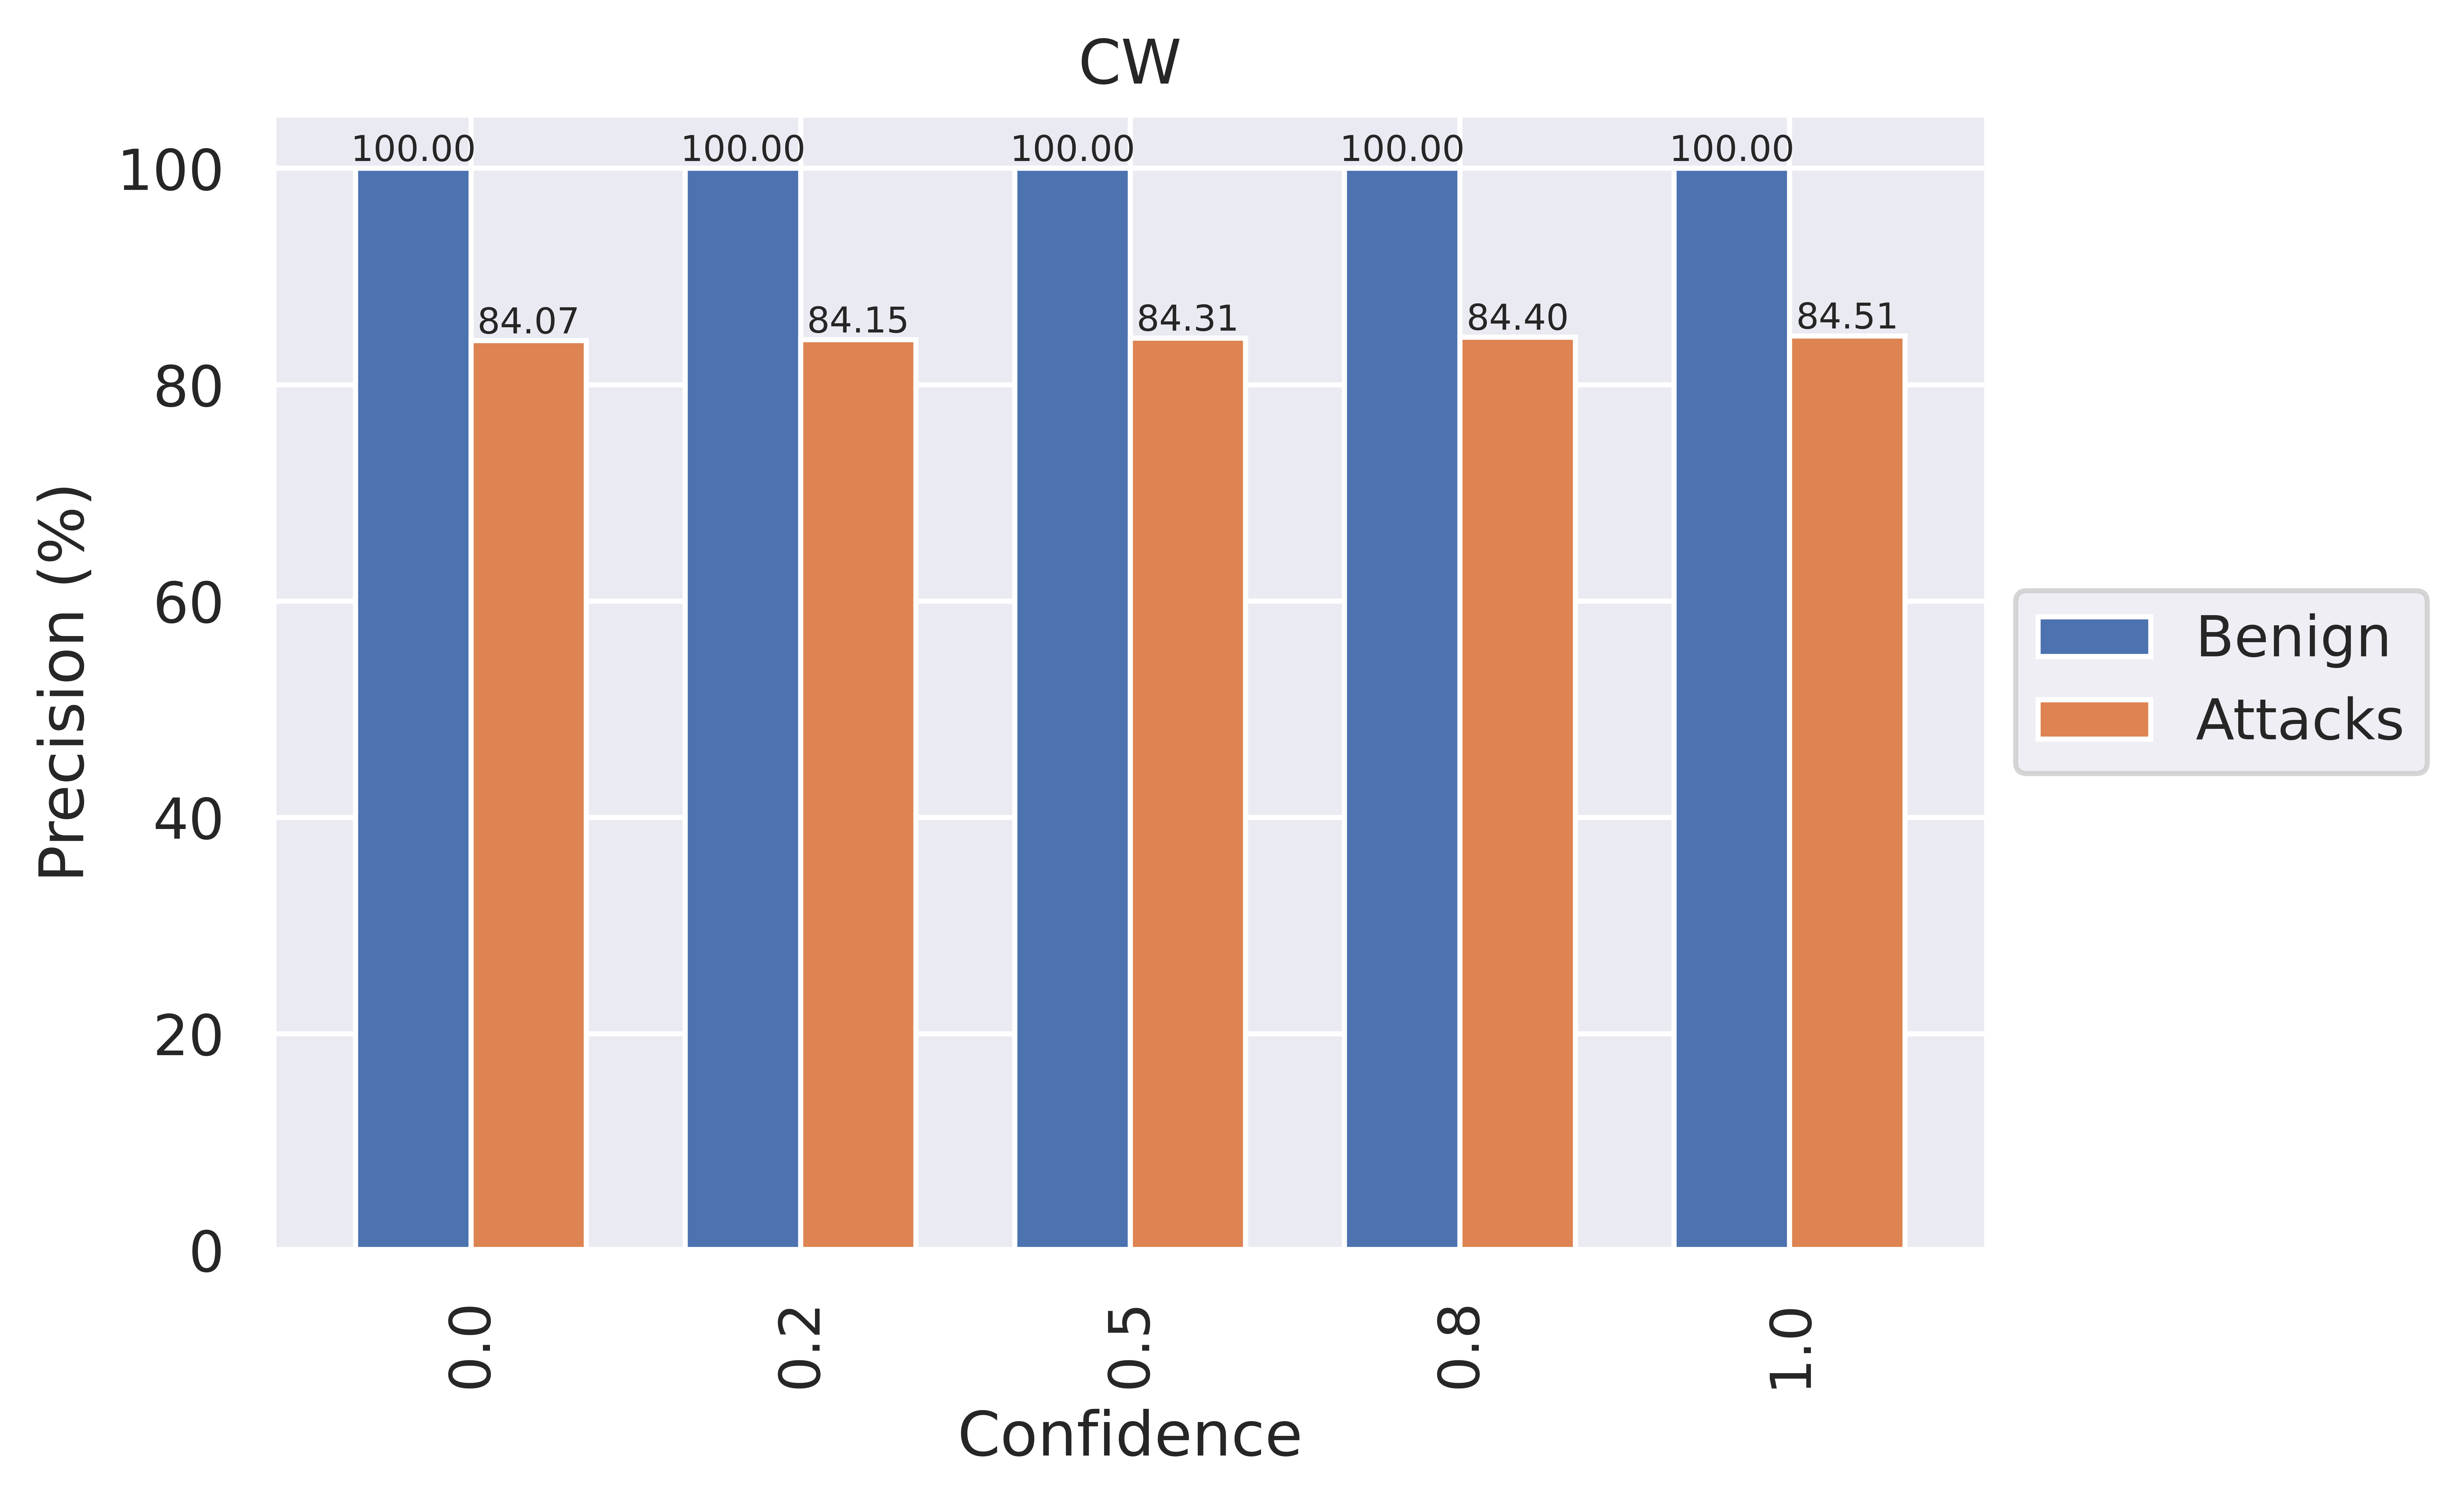
\includegraphics[width=\textwidth]{/home/wojtyla/Documentos/Artigo_2023/IJCNN_Suplementary/Figures/UNSW_Clean_CW_bin_paper.png}
			%caption{Figure}
			\label{fig:1}
		\end{subfigure}
		\hfill
		\begin{subfigure}[b]{0.45\textwidth}
			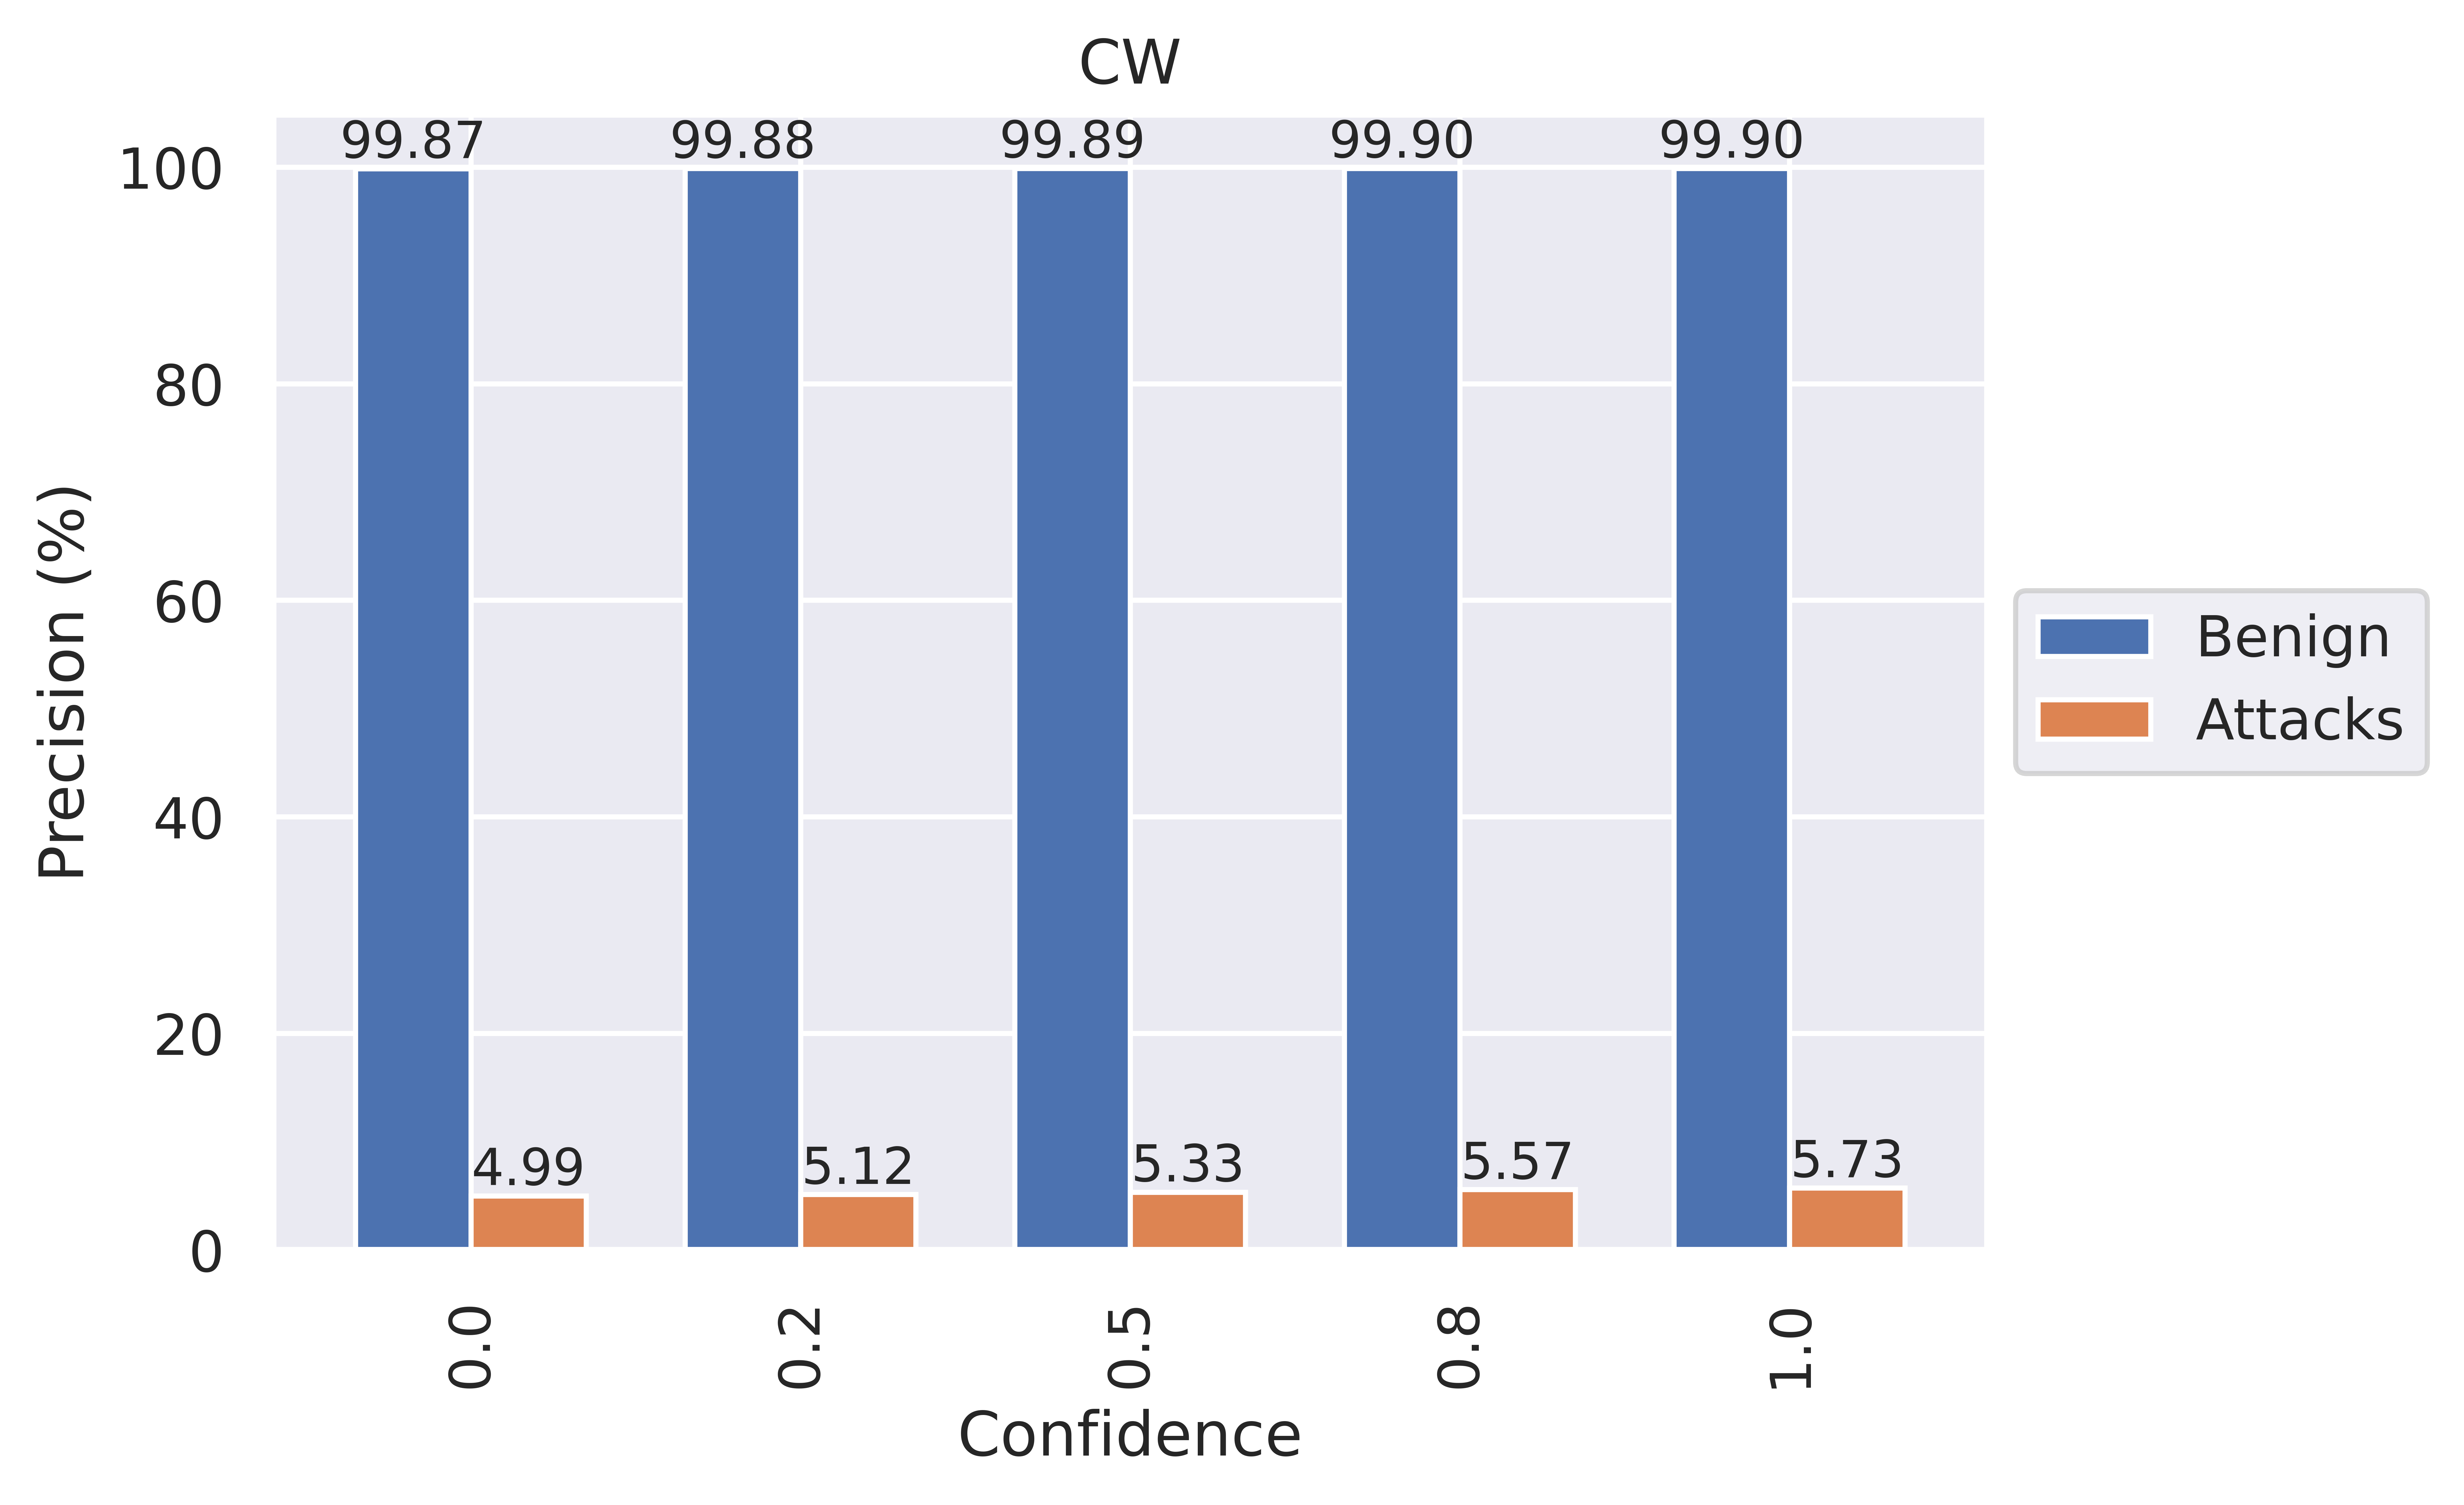
\includegraphics[width=\textwidth]{/home/wojtyla/Documentos/Artigo_2023/IJCNN_Suplementary/Figures/UNSW_IDS_CW_bin_paper.png}
			%caption{Figure}
			\label{fig:4}
		\end{subfigure}
		\caption{Plots for CW-2 attack on binary models with UNSW-NB15.Left:EnC model; Right:EnIDS model.}
		\label{fig:unsw_cw_bin}
	\end{figure}
	
	
	\begin{table}[H]
		\caption{CW-2 attack against EnC and EnIDS for multiclass classification on the UNSW-NB15 dataset.}
		\small
		\setlength{\tabcolsep}{0.7pt}
		\centering
		\label{tab:unsw_multi_cw}
		\hspace*{-1.7cm}		
		\begin{tabular}{|c|c|c|c|c|c|c|c|c|c|c|c|c|c|c|c|c|}
			\hline
			\multirow{4}{*}{\textbf{Type}} & \multirow{4}{*}{\textbf{Metric}}& \multicolumn{15}{c|}{\textbf{Confidence}} \\
			\cline{3-17}
			&  & \multicolumn{3}{c|}{\textbf{0.0}} & \multicolumn{3}{c|}{\textbf{0.2}} & \multicolumn{3}{c|}{\textbf{0.5}} & \multicolumn{3}{c|}{\textbf{0.8}} & \multicolumn{3}{c|}{\textbf{1.0}} 
			\\
			\cline{3-17}
			&  & \textbf{\textsl{Normal}} & \textbf{\textsl{Recon.}} & \textbf{\textsl{Generic}} & \textbf{\textsl{Normal}} & \textbf{\textsl{Recon.}} & \textbf{\textsl{Generic}} & \textbf{\textsl{Normal}} & \textbf{\textsl{Recon.}} & \textbf{\textsl{Generic}} & \textbf{\textsl{Normal}} & \textbf{\textsl{Recon.}} & \textbf{\textsl{Generic}} & \textbf{\textsl{Normal}} & \textbf{\textsl{Recon.}} & \textbf{\textsl{Generic}}
			\\
			\hline
			\multirow{3}{*}{EnC} & Precision & 100.00 & 32.34 & 100.00 & 100.00 & 33.53 & 100.00 & 100.00 & 34.13 & 100.00 & 100.00 & 34.13 & 100.00 & 100.00 & 34.32 & 100.00
			\\
			
			& Recall & 70.09 & 15.34 & 84.77 & 70.12 & 16.19 & 85.44 & 70.20 & 16.19 & 86.44 & 70.30 & 16.19 & 87.50 & 70.36 & 16.48 & 87.90
			\\
			
			& ROC-AUC & 98.92 & 98.34 & 99.03 & 98.91 & 98.26 & 99.02 & 98.91 & 98.22 & 99.01 & 98.90 & 98.20 & 99.00 & 98.89 & 98.16 & 99.00
			\\
			\hline
			\multirow{3}{*}{EnIDS} & Precision & \cellcolor{blue!20}100.00 & 13.78 & 97.46 & \cellcolor{blue!20}100.00 & 14.74 & 97.82 & \cellcolor{blue!20}100.00 & 18.81 & 97.75 & \cellcolor{blue!20}100.00 & 21.23 & 97.75 & \cellcolor{blue!20}100.00 & 24.63 & 98.03
			\\
			
			& Recall & \cellcolor{yellow!50}99.59 & 12.22 & \cellcolor{yellow!50}89.43 & \cellcolor{yellow!50}99.59 & 13.07 & \cellcolor{yellow!50}89.43 & \cellcolor{yellow!50}99.59 & 17.05 & \cellcolor{yellow!50}89.56 & \cellcolor{yellow!50}99.59 & 19.60 & \cellcolor{yellow!50}89.56 & \cellcolor{yellow!50}99.59 & 23.58 & \cellcolor{yellow!50}89.56
			\\
			
			& ROC-AUC & \cellcolor{yellow!50}99.92 & \cellcolor{yellow!50}99.82 & \cellcolor{yellow!50}99.94 & \cellcolor{yellow!50}99.92 & \cellcolor{yellow!50}99.81 & \cellcolor{yellow!50}99.94 & \cellcolor{yellow!50}99.92 & \cellcolor{yellow!50}99.80 & \cellcolor{yellow!50}99.94 & \cellcolor{yellow!50}99.92 & \cellcolor{yellow!50}99.80 & \cellcolor{yellow!50}99.94 & \cellcolor{yellow!50}99.92 & \cellcolor{yellow!50}99.80 & \cellcolor{yellow!50}99.94
			\\
			\hline
		\end{tabular}		
	\end{table}
	
	
	\begin{figure}[H]
		\centering
		\begin{subfigure}[b]{0.45\textwidth}
			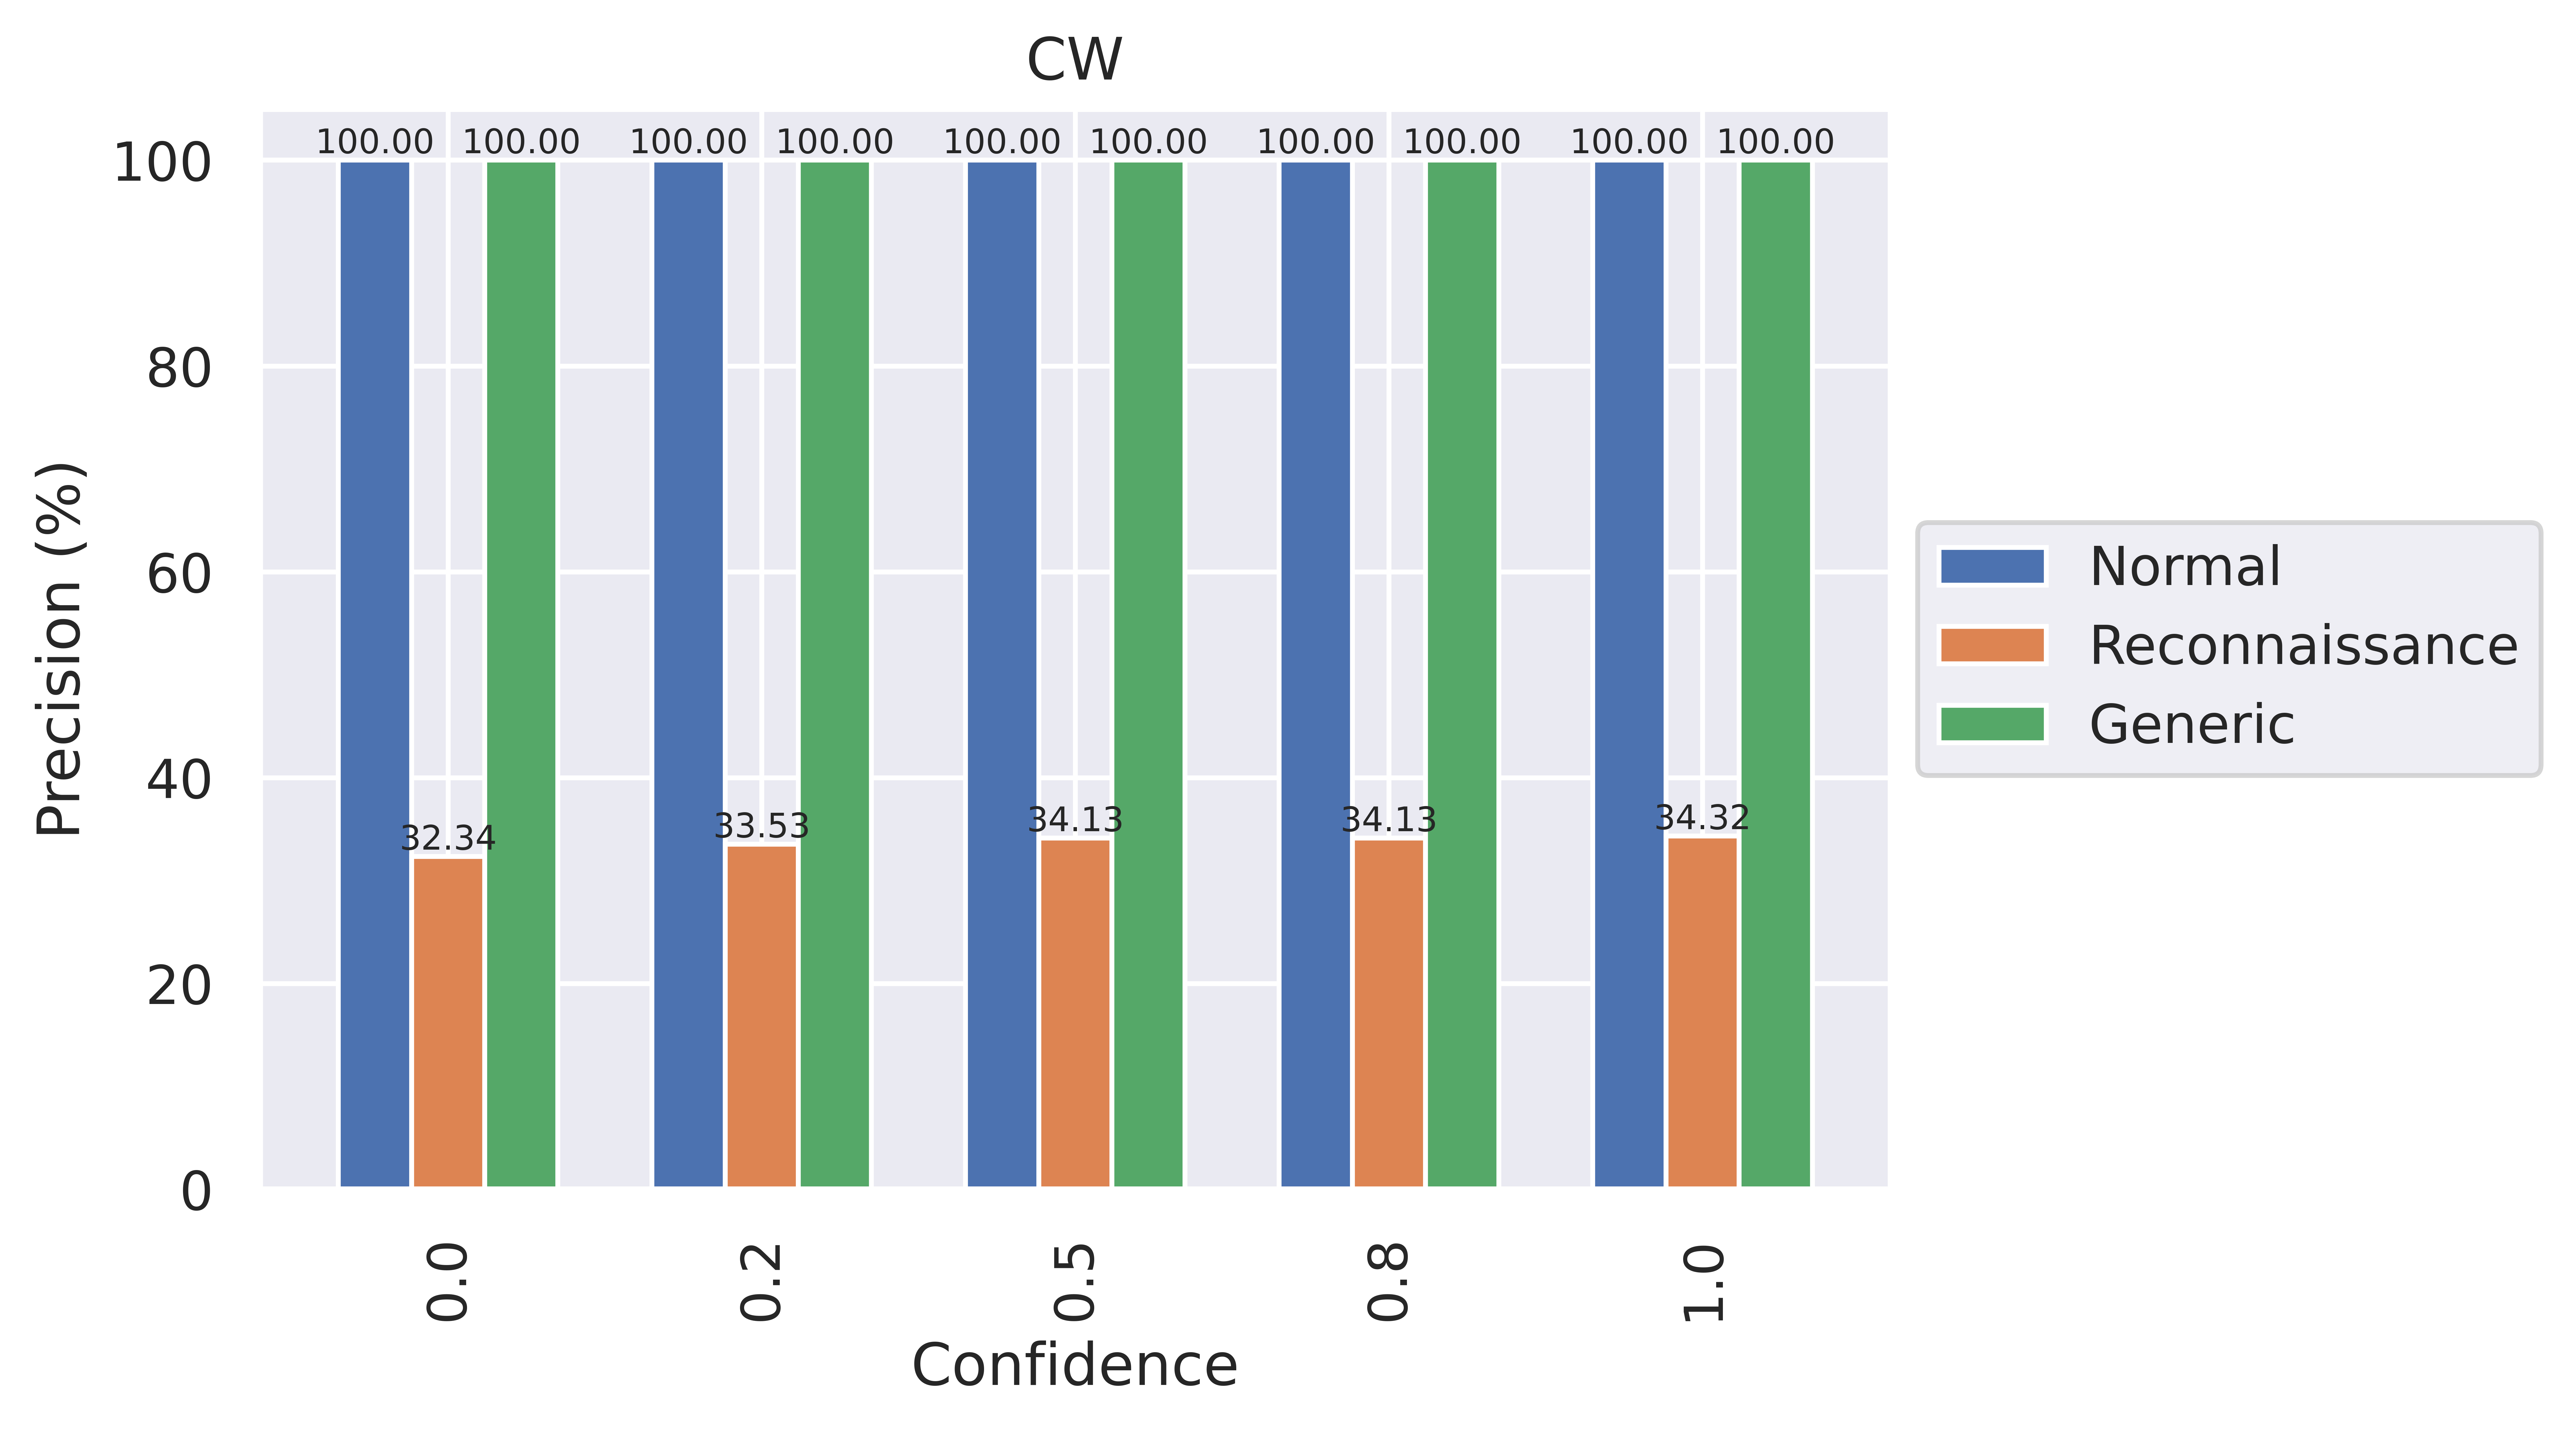
\includegraphics[width=\textwidth]{/home/wojtyla/Documentos/Artigo_2023/IJCNN_Suplementary/Figures/UNSW_Clean_CW_multi_paper.png}
			%caption{Figure}
			\label{fig:1}
		\end{subfigure}
		\hfill
		\begin{subfigure}[b]{0.45\textwidth}
			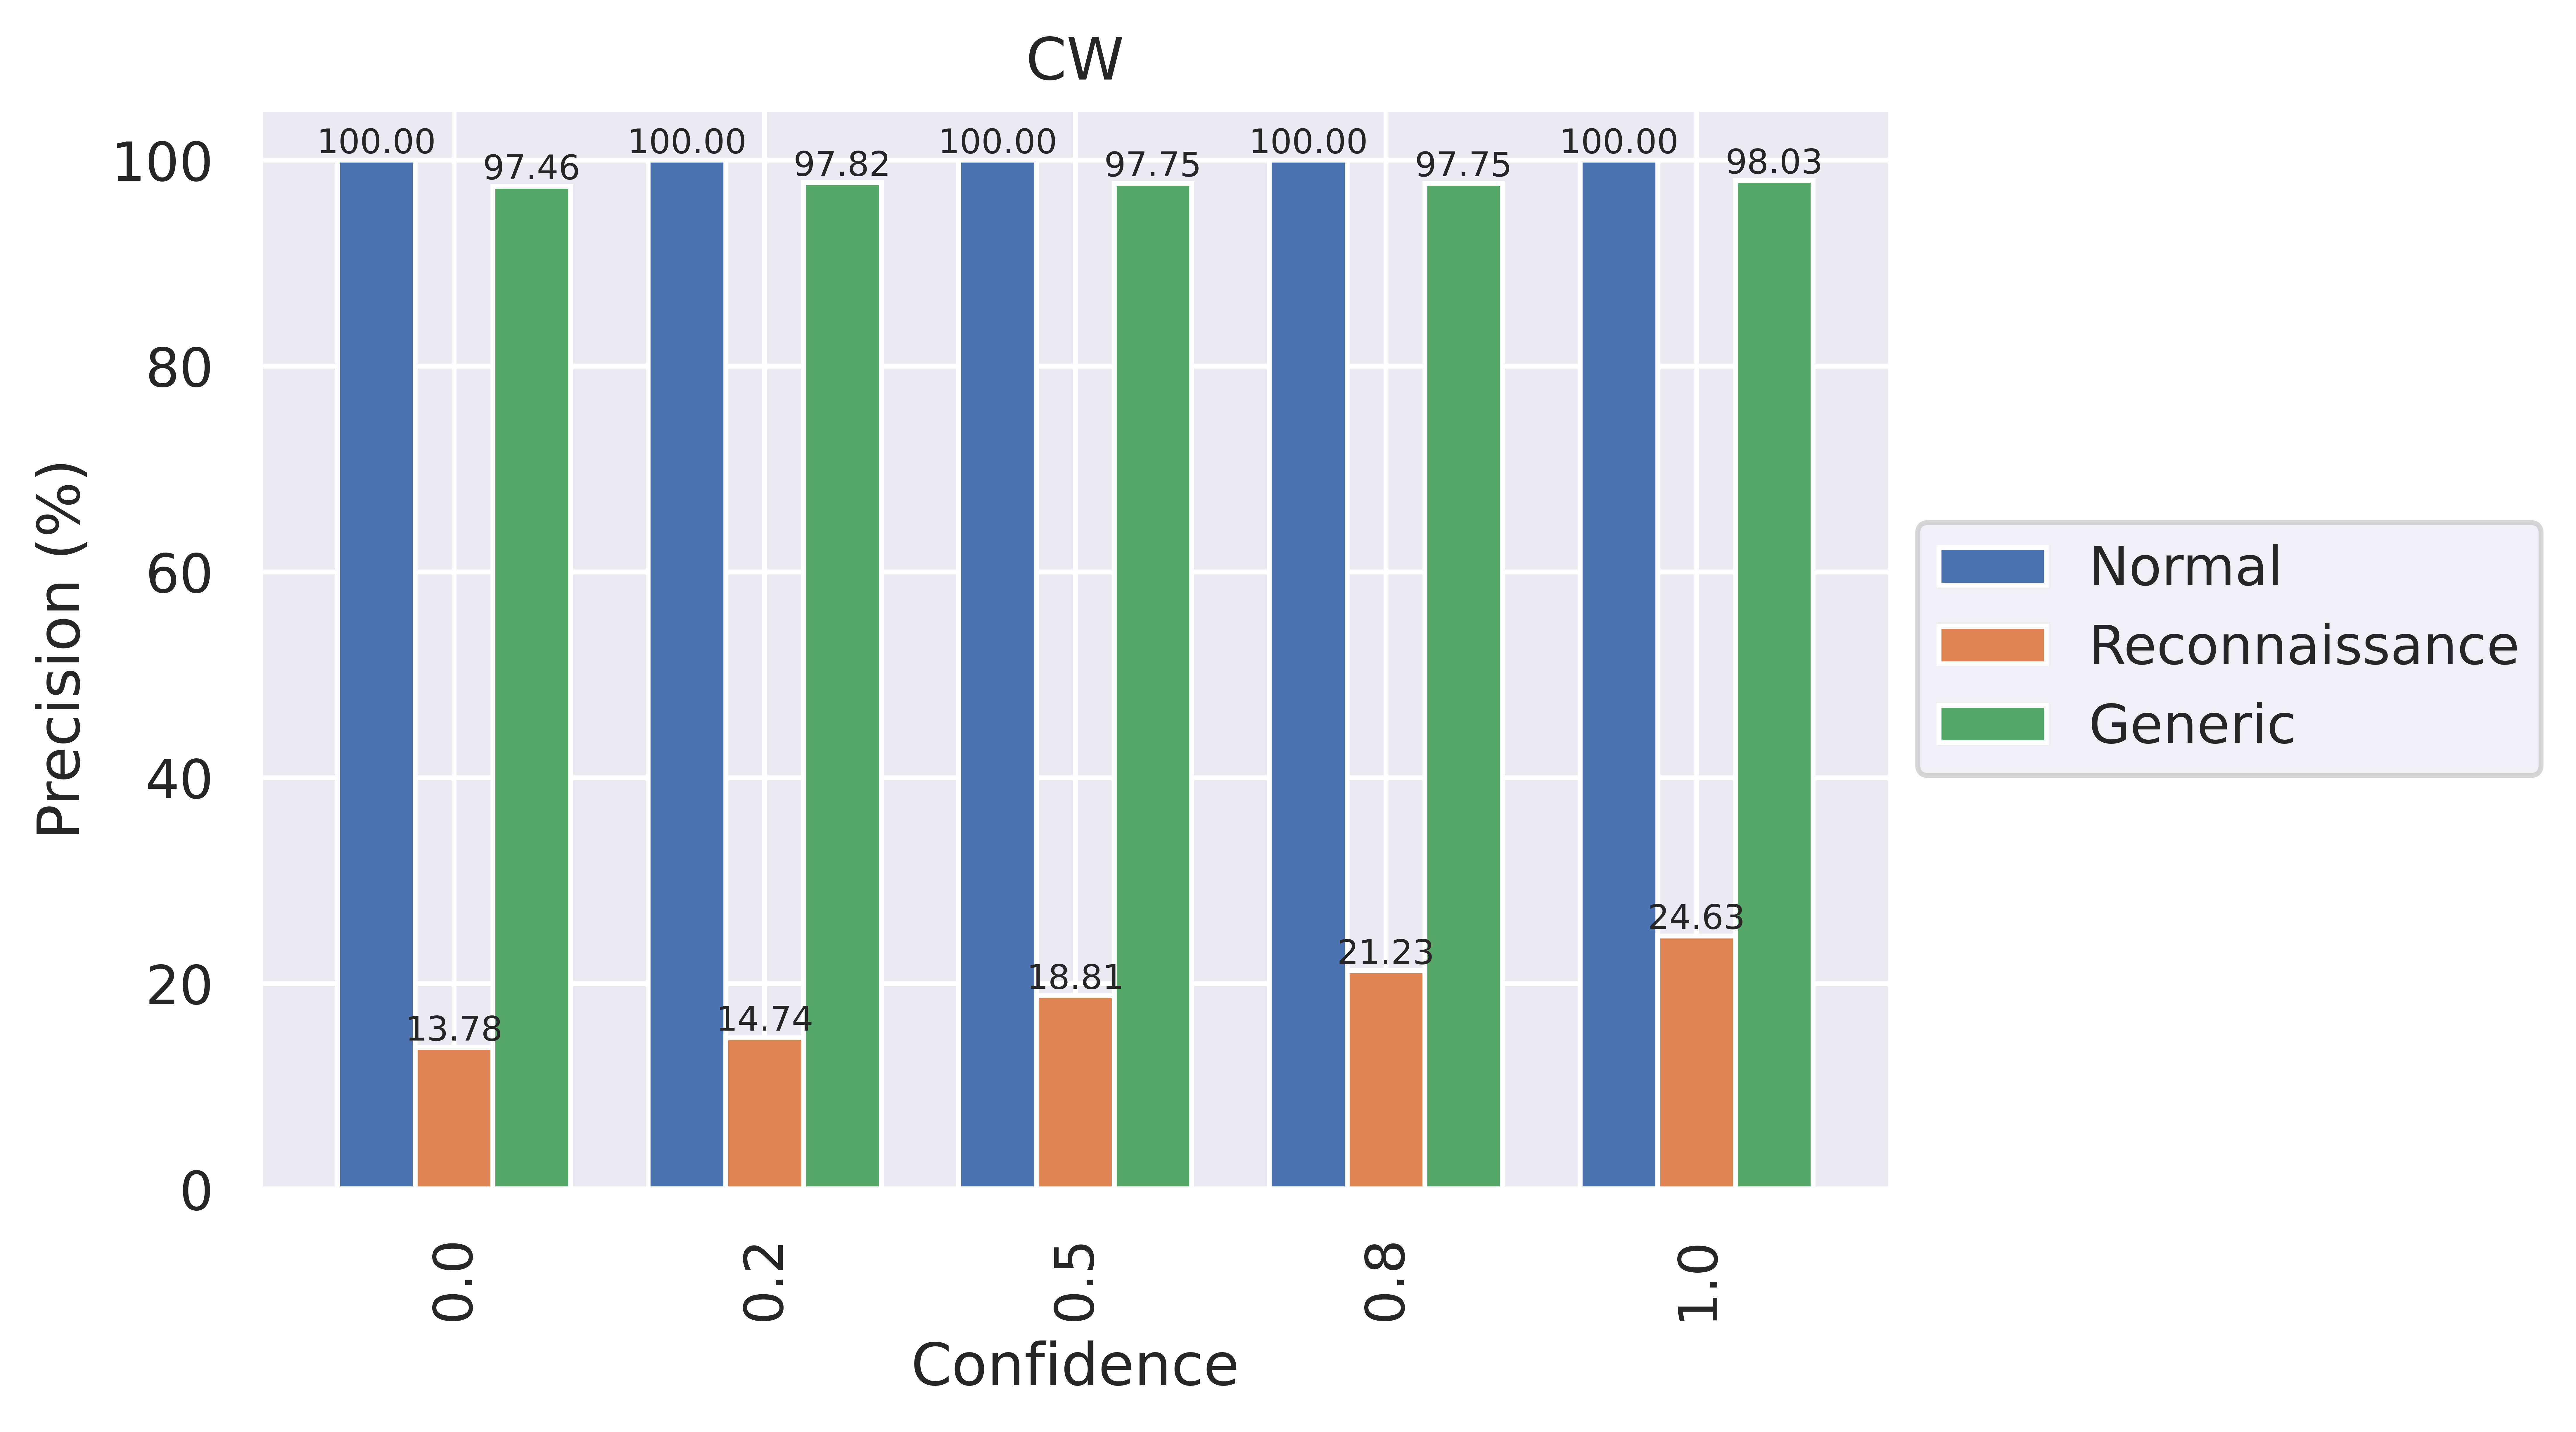
\includegraphics[width=\textwidth]{/home/wojtyla/Documentos/Artigo_2023/IJCNN_Suplementary/Figures/UNSW_IDS_CW_multi_paper.png}
			%caption{Figure}
			\label{fig:4}
		\end{subfigure}
		\caption{Plots for CW-2 attack on multiclass models with UNSW-NB15.Left:EnC model; Right:EnIDS model.}
		\label{fig:unsw_cw_multi}
	\end{figure}
	
	
	\section{DeepFool (DF-2)}
	
	\subsection{CIC IDS2017}
	
	\begin{table}[H]
		\caption{DF-2 attack against EnC and EnIDS for binary classification on the CIC IDS2017 dataset.}
		\small
		\setlength{\tabcolsep}{1pt}
		\centering
		\label{tab:cic_bin_df}
		
		\begin{tabular}{|c|c|c|c|c|c|c|c|c|c|c|c|}
			\hline
			\multirow{4}{*}{\textbf{Type}} & \multirow{4}{*}{\textbf{Metric}}& \multicolumn{10}{c|}{\textbf{Confidence}} \\
			\cline{3-12}
			&  & \multicolumn{2}{c|}{\textbf{0.001}} & \multicolumn{2}{c|}{\textbf{0.002}} & \multicolumn{2}{c|}{\textbf{0.005}} & \multicolumn{2}{c|}{\textbf{0.008}} & \multicolumn{2}{c|}{\textbf{0.009}}   \\
			\cline{3-12}
			&  &  \textbf{\textsl{Benign}} & \textbf{\textsl{Attacks}} & \textbf{\textsl{Benign}} & \textbf{\textsl{Attacks}} & \textbf{\textsl{Benign}} & \textbf{\textsl{Attacks}} & \textbf{\textsl{Benign}} & \textbf{\textsl{Attacks}} & \textbf{\textsl{Benign}} & \textbf{\textsl{Attacks}} \\
			\hline
			\multirow{3}{*}{EnC}& Precision & 77.28 & 0.75 & 77.26 & 0.74 & 77.19 & 0.74 & 77.12 & 0.73 & 77.09 & 0.72
			\\
			
			& Recall & 68.51 & 1.16 & 68.45 & 1.16 & 68.17 & 1.16 & 67.89 & 1.15 & 67.78 & 1.15
			\\
			
			& ROC-AUC & 1.74 & 1.72 & 1.73 & 1.72 & 1.72 & 1.70 & 1.70 & 1.68 & 1.69 & 1.68
			\\
			\hline
			\multirow{3}{*}{EnIDS} & Precision & \cellcolor{yellow!50}94.48 & \cellcolor{yellow!50}60.21 & \cellcolor{yellow!50}94.47 & \cellcolor{yellow!50}60.16 & \cellcolor{yellow!50}94.44 & \cellcolor{yellow!50}60.02 & \cellcolor{yellow!50}94.41 & \cellcolor{yellow!50}59.89 & \cellcolor{yellow!50}94.40 & \cellcolor{yellow!50}59.84
			\\
			
			& Recall & \cellcolor{yellow!50}90.00 & \cellcolor{yellow!50}74.21 & \cellcolor{yellow!50}89.99 & \cellcolor{yellow!50}74.17 & \cellcolor{yellow!50}89.95 & \cellcolor{yellow!50}73.99 & \cellcolor{yellow!50}89.92 & \cellcolor{yellow!50}73.86 & \cellcolor{yellow!50}89.91 & \cellcolor{yellow!50}73.81
			\\
			
			& ROC-AUC & \cellcolor{yellow!50}92.98 & \cellcolor{yellow!50}92.98 & \cellcolor{yellow!50}92.96 & \cellcolor{yellow!50}92.96 & \cellcolor{yellow!50}92.89 & \cellcolor{yellow!50}92.89 & \cellcolor{yellow!50}92.82 & \cellcolor{yellow!50}92.82 & \cellcolor{yellow!50}92.80 & \cellcolor{yellow!50}92.80
			\\
			\hline
		\end{tabular}
		
	\end{table}
	
	\begin{figure}[H]
		\centering
		\begin{subfigure}[b]{0.45\textwidth}
			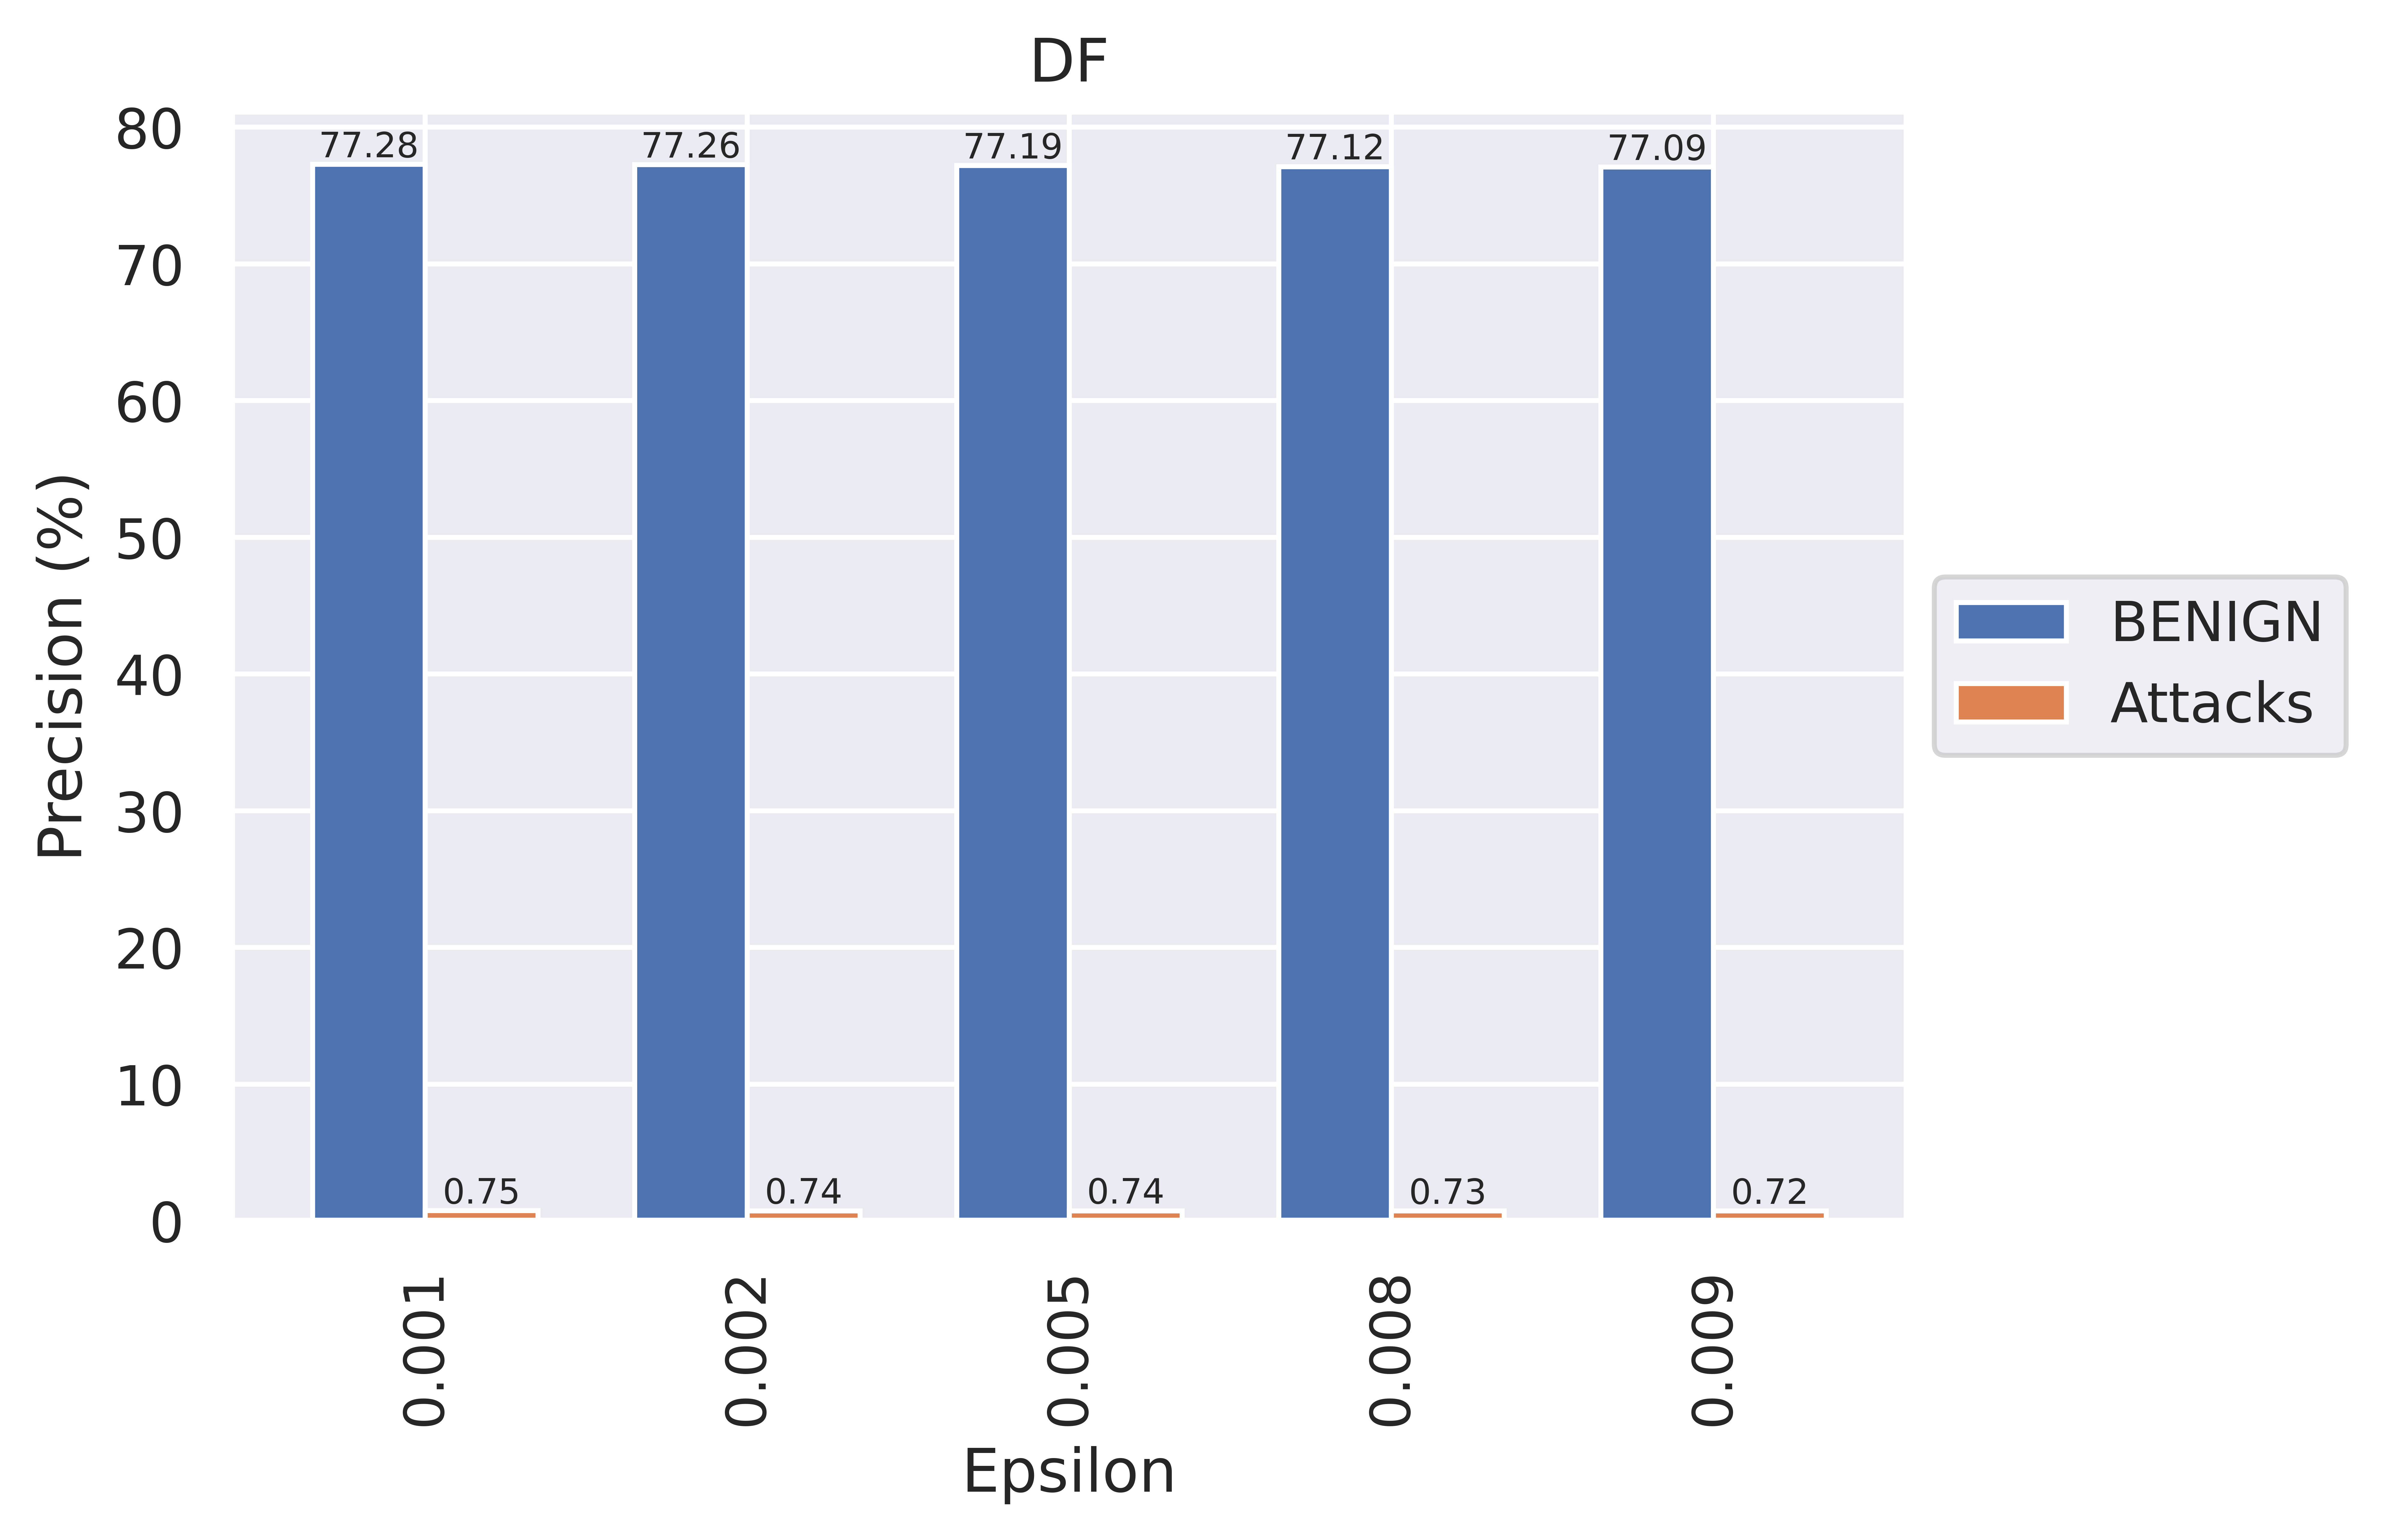
\includegraphics[width=\textwidth]{/home/wojtyla/Documentos/Artigo_2023/IJCNN_Suplementary/Figures//CIC_Clean_DF_bin_paper.png}
			%caption{Figure}
			\label{fig:1}
		\end{subfigure}
		\hfill
		\begin{subfigure}[b]{0.45\textwidth}
			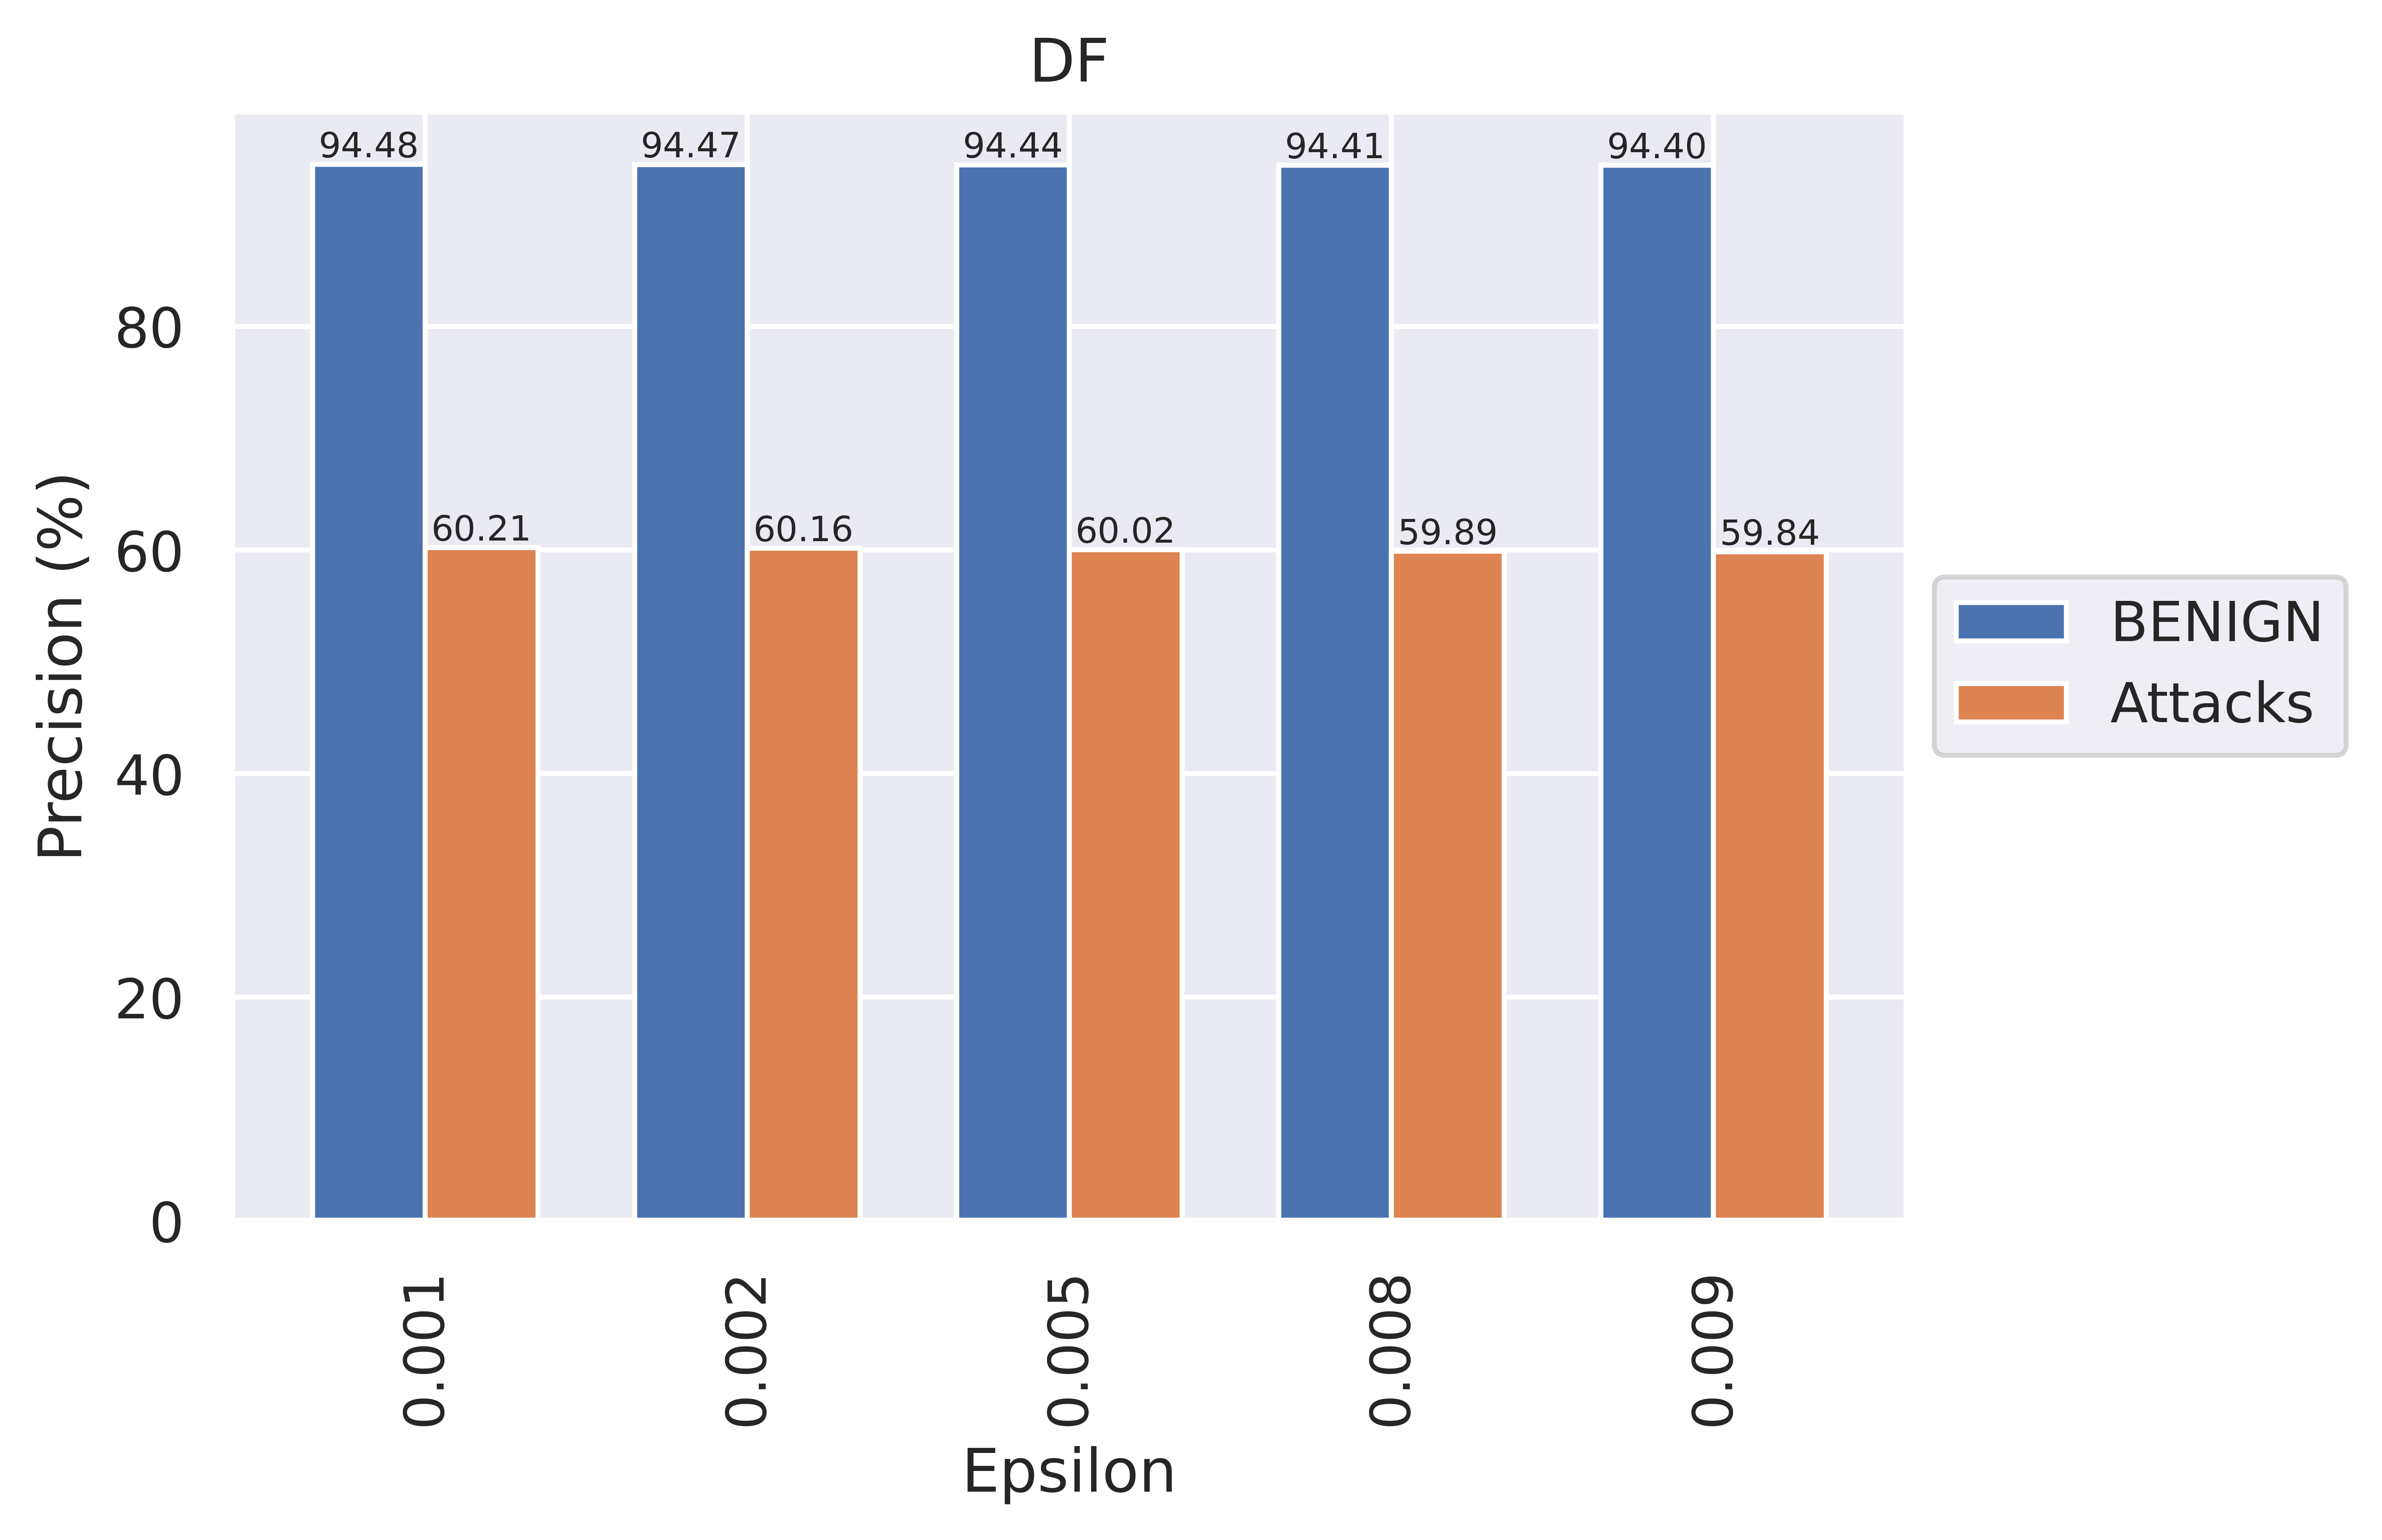
\includegraphics[width=\textwidth]{/home/wojtyla/Documentos/Artigo_2023/IJCNN_Suplementary/Figures//CIC_IDS_DF_bin_paper.png}
			%caption{Figure}
			\label{fig:4}
		\end{subfigure}
		\caption{Plots for DF-2 attack on binary models with CIC IDS2017.Left:EnC model; Right:EnIDS model.}
		\label{fig:cic_df_bin}
	\end{figure}
	
	
	\begin{table}[H]
		\caption{DF-2 attack against EnC and EnIDS for multiclass classification on the CIC IDS2017 dataset.}
		\small
		\setlength{\tabcolsep}{1pt}
		\centering
		\label{tab:cic_multi_df}
		\hspace*{-2.3cm}
		
		\begin{tabular}{|c|c|c|c|c|c|c|c|c|c|c|c|c|c|c|c|c|}
			\hline
			\multirow{4}{*}{\textbf{Type}} & \multirow{4}{*}{\textbf{Metric}}& \multicolumn{15}{c|}{\textbf{Epsilon ($\epsilon$)}} \\
			\cline{3-17}
			&  & \multicolumn{3}{c|}{\textbf{0.001}} & \multicolumn{3}{c|}{\textbf{0.002}} & \multicolumn{3}{c|}{\textbf{0.005}} & \multicolumn{3}{c|}{\textbf{0.008}} & \multicolumn{3}{c|}{\textbf{0.009}}  \\
			\cline{3-17}
			&  & \textbf{\textsl{Benign}} & \textbf{\textsl{DoS}} & \textbf{\textsl{DDoS}} & \textbf{\textsl{Benign}} & \textbf{\textsl{DoS}} & \textbf{\textsl{DDoS}} & \textbf{\textsl{Benign}} & \textbf{\textsl{DoS}} & \textbf{\textsl{DDoS}} & \textbf{\textsl{Benign}} & \textbf{\textsl{DoS}} & \textbf{\textsl{DDoS}} & \textbf{\textsl{Benign}} & \textbf{\textsl{DoS}} & \textbf{\textsl{DDoS}} \\
			\hline
			\multirow{3}{*}{EnC} & Precision & 66.67 & 0.18 & 1.95 & 66.52 & 0.17 & 1.90 & 66.11 & 0.17 & 1.70 & 65.66 & 0.17 & 1.54 & 65.49 & 0.16 & 1.48
			\\
			
			& Recall & 25.43 & 0.41 & 1.12 & 25.28 & 0.41 & 1.10 & 24.83 & 0.40 & 1.00 & 24.35 & 0.39 & 0.92 & 24.17 & 0.38 & 0.89
			\\
			
			& ROC-AUC & 27.69 & 7.11 & 93.96 & 27.63 & 7.08 & 93.92 & 27.44 & 7.00 & 93.80 & 27.27 & 6.92 & 93.68 & 27.21 & 6.90 & 93.64
			\\
			\hline
			\multirow{3}{*}{EnIDS} & Precision & \cellcolor{yellow!50}96.87 & \cellcolor{yellow!50}69.88 & \cellcolor{yellow!50}95.19 & \cellcolor{yellow!50}96.87 & \cellcolor{yellow!50}69.86 & \cellcolor{yellow!50}95.18 & \cellcolor{yellow!50}96.86 & \cellcolor{yellow!50}69.79 & \cellcolor{yellow!50}95.14 & \cellcolor{yellow!50}96.86 & \cellcolor{yellow!50}69.72 & \cellcolor{yellow!50}95.12 & \cellcolor{yellow!50}96.85 & \cellcolor{yellow!50}69.68 & \cellcolor{yellow!50}95.11
			\\
			
			& Recall & \cellcolor{yellow!50}92.12 & \cellcolor{yellow!50}69.46 & \cellcolor{yellow!50}92.51 & \cellcolor{yellow!50}92.11 & \cellcolor{yellow!50}69.44 & \cellcolor{yellow!50}92.48 & \cellcolor{yellow!50}92.09 & \cellcolor{yellow!50}69.38 & \cellcolor{yellow!50}92.46 & \cellcolor{yellow!50}92.05 & \cellcolor{yellow!50}69.32 & \cellcolor{yellow!50}92.41 & \cellcolor{yellow!50}92.04 & \cellcolor{yellow!50}69.28 & \cellcolor{yellow!50}92.38
			\\
			
			& ROC-AUC & \cellcolor{yellow!50}95.73 & \cellcolor{yellow!50}95.62 & \cellcolor{yellow!50}99.36 & \cellcolor{yellow!50}95.72 & \cellcolor{yellow!50}95.61 & \cellcolor{yellow!50}99.35 & \cellcolor{yellow!50}95.71 & \cellcolor{yellow!50}95.60 & \cellcolor{yellow!50}99.35 & \cellcolor{yellow!50}95.71 & \cellcolor{yellow!50}95.58 & \cellcolor{yellow!50}99.34 & \cellcolor{yellow!50}95.70 & \cellcolor{yellow!50}95.57 & \cellcolor{yellow!50}99.34
			\\
			\hline
		\end{tabular}	
	\end{table}
	
	\begin{figure}[H]
		\centering
		\begin{subfigure}[b]{0.45\textwidth}
			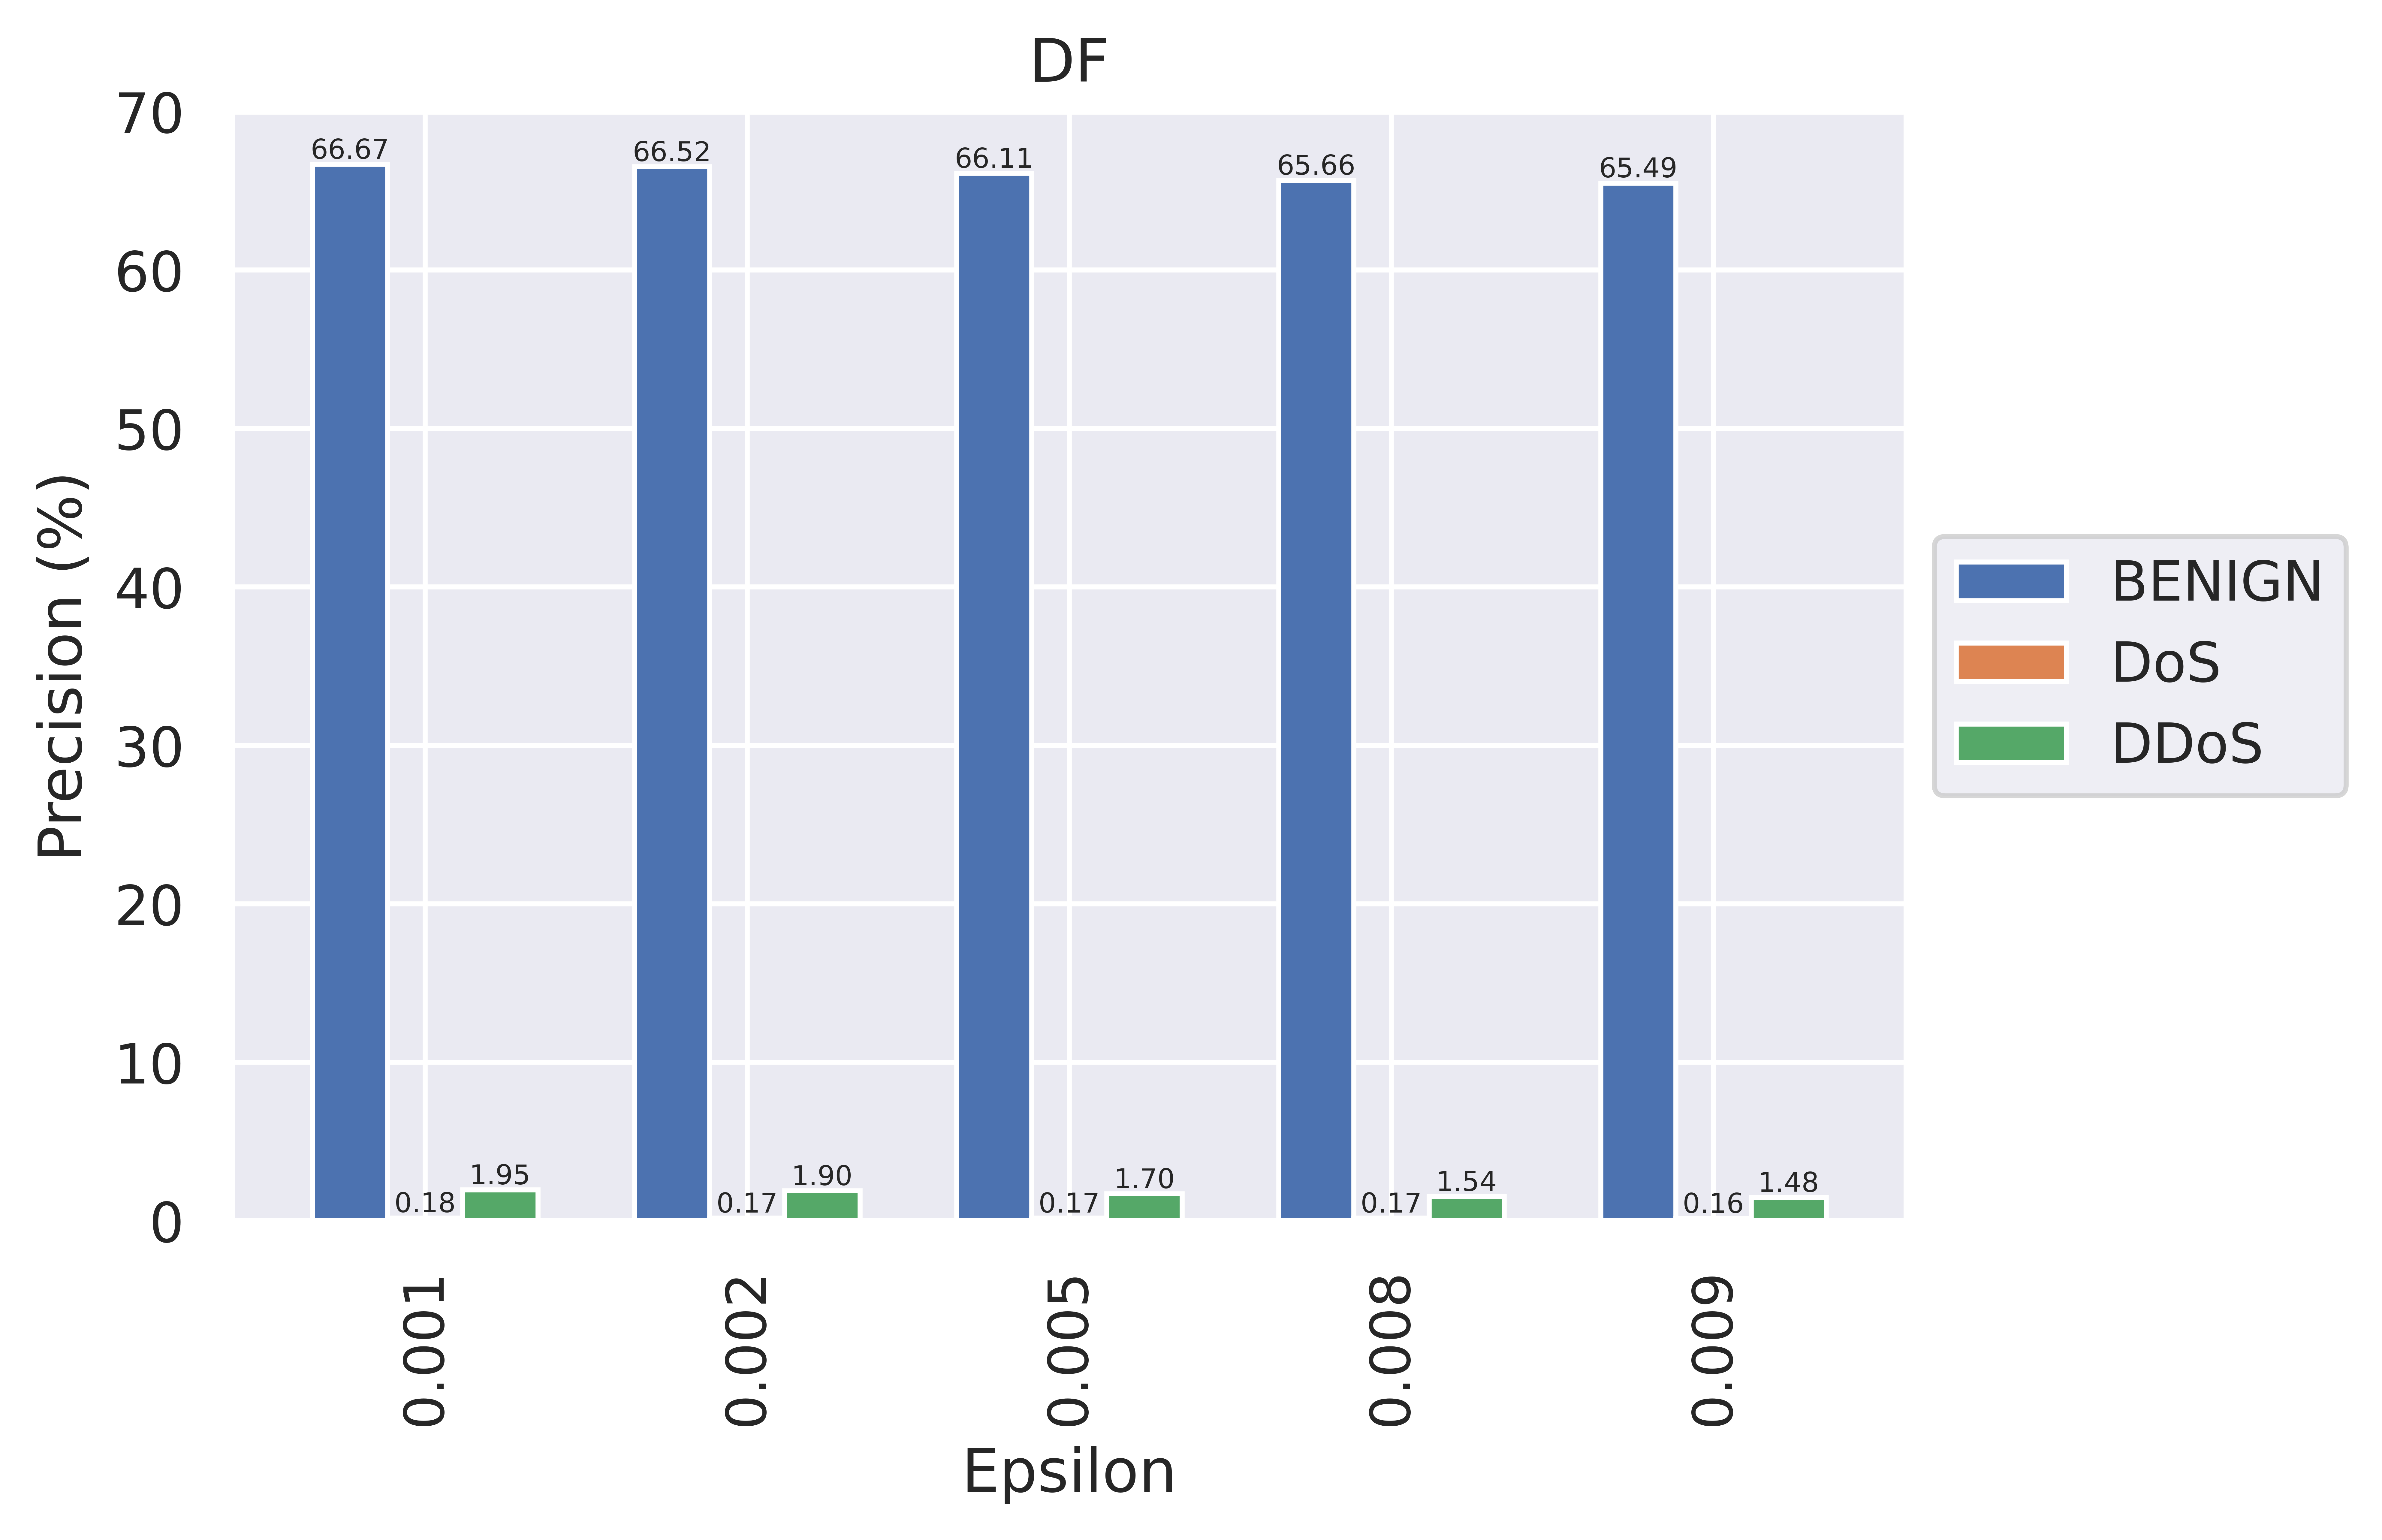
\includegraphics[width=\textwidth]{/home/wojtyla/Documentos/Artigo_2023/IJCNN_Suplementary/Figures//CIC_Clean_DF_multi_paper.png}
			%caption{Figure}
			\label{fig:1}
		\end{subfigure}
		\hfill
		\begin{subfigure}[b]{0.45\textwidth}
			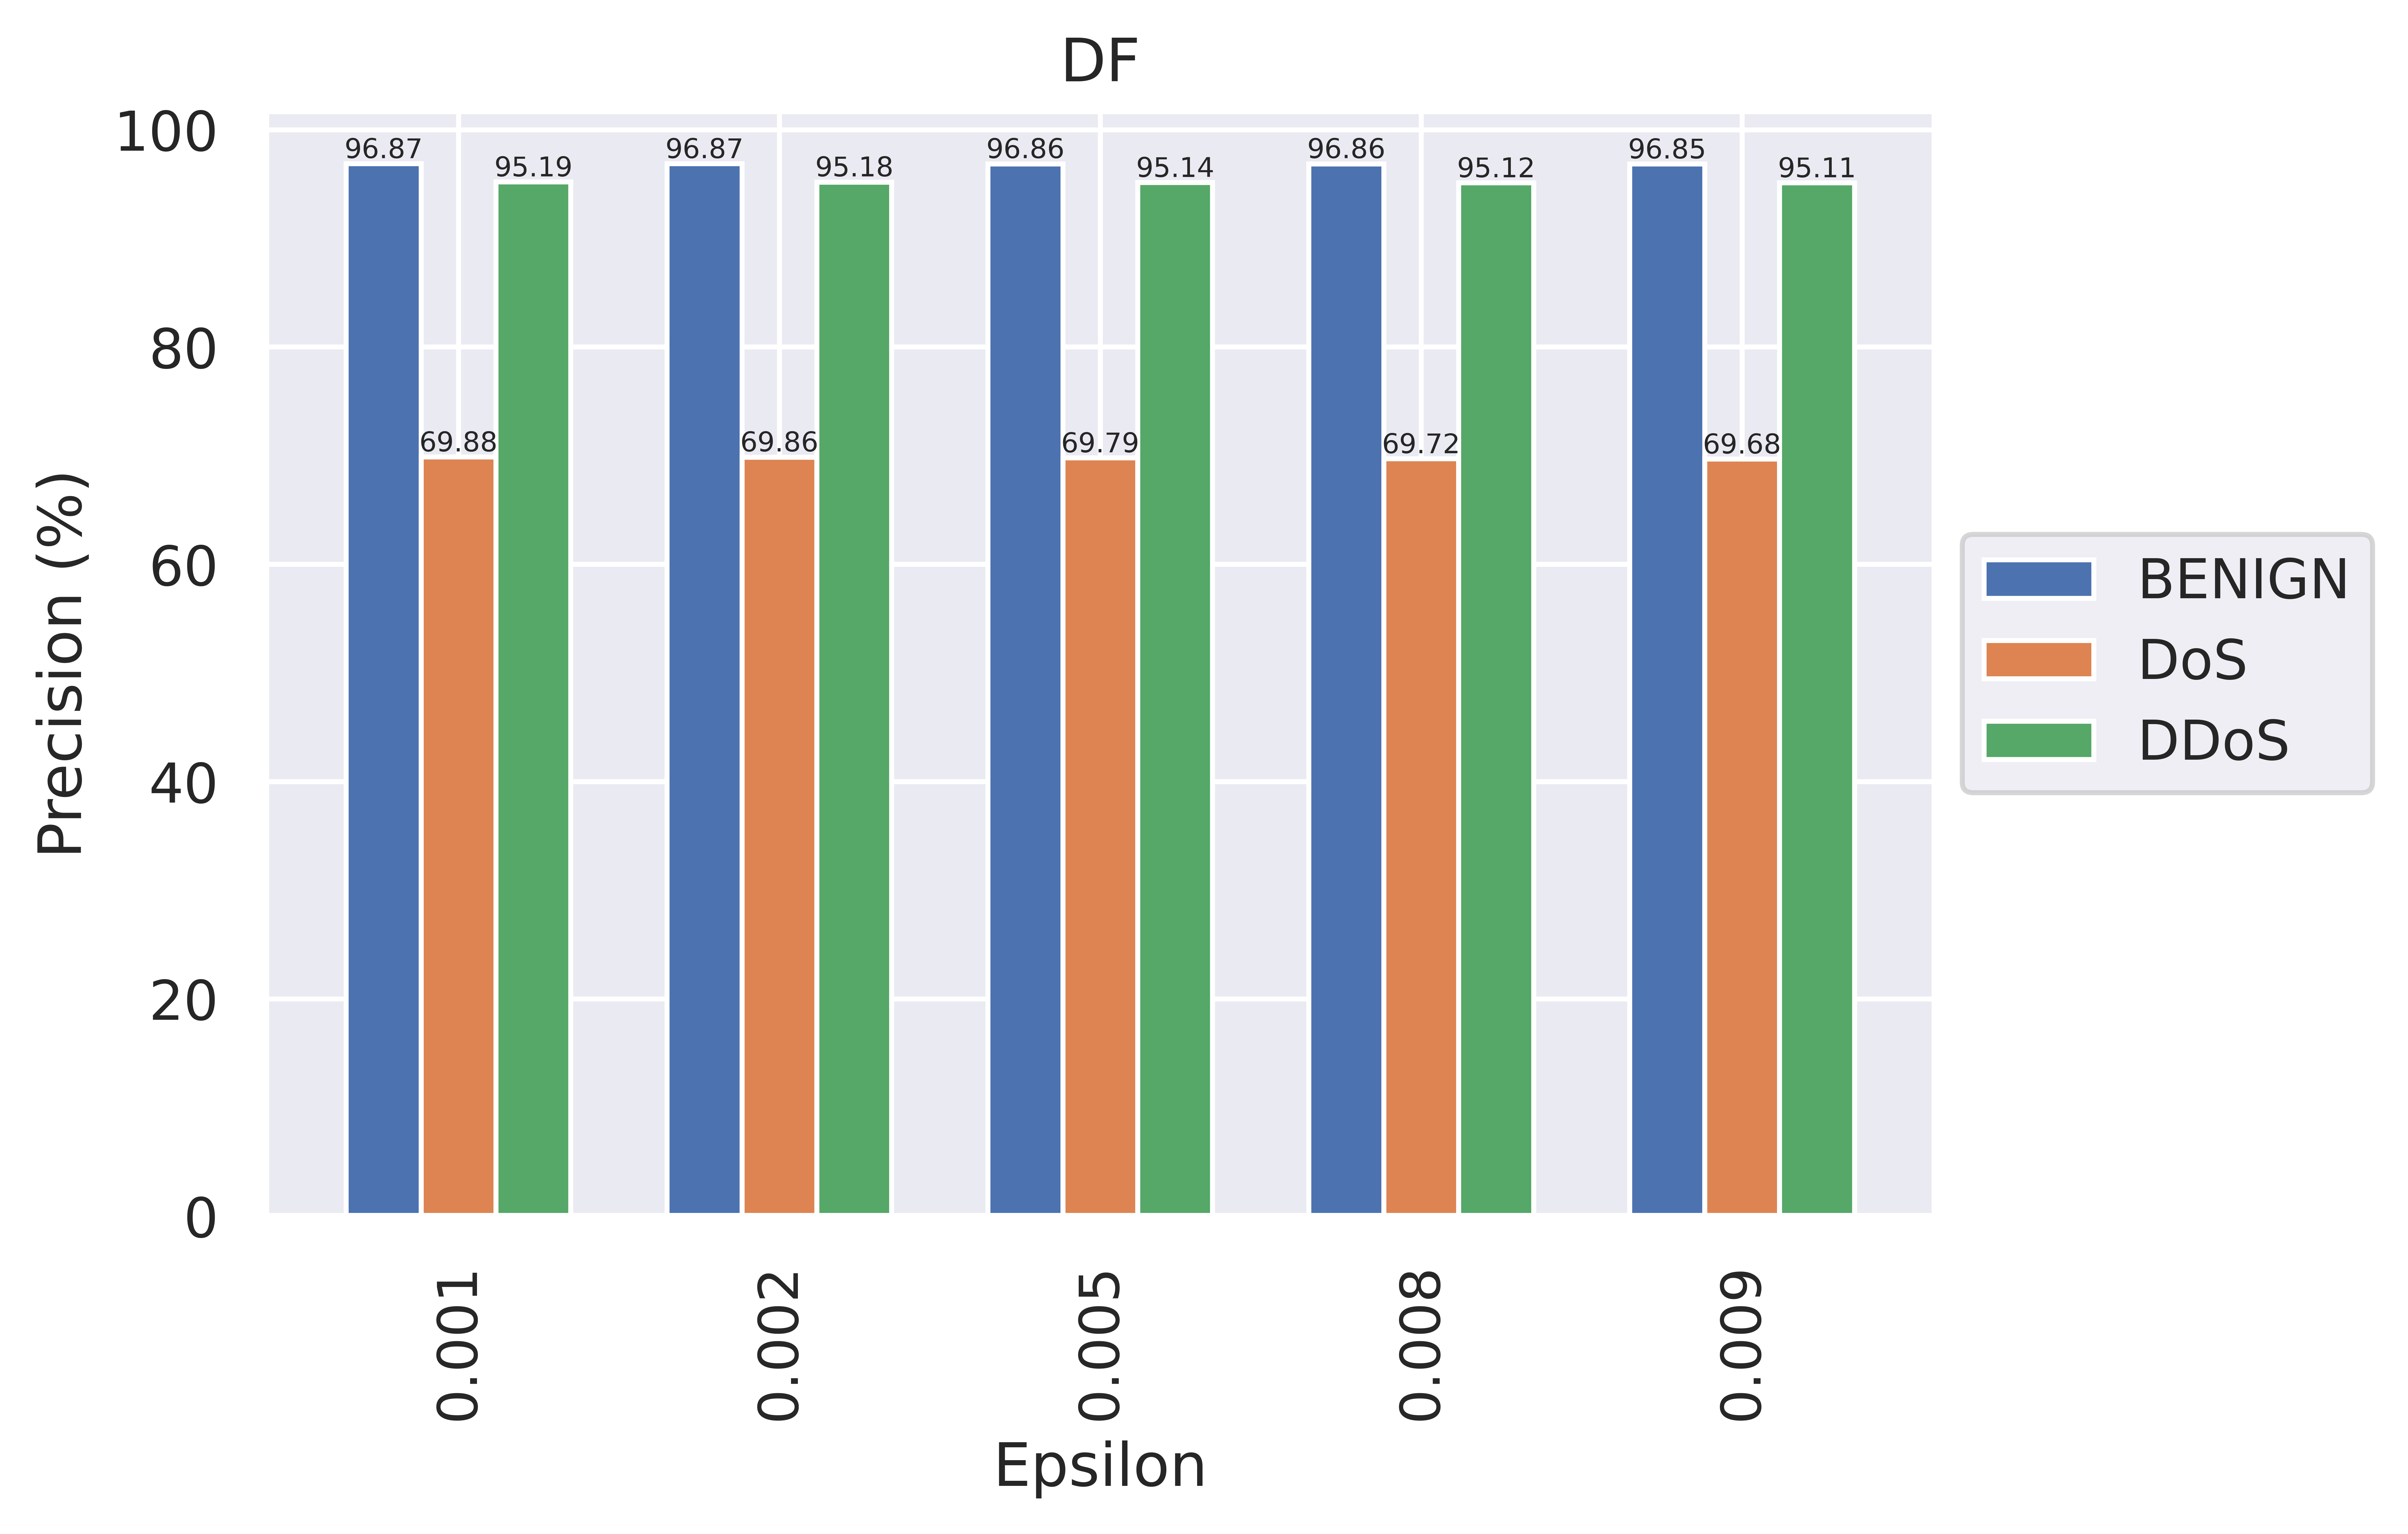
\includegraphics[width=\textwidth]{/home/wojtyla/Documentos/Artigo_2023/IJCNN_Suplementary/Figures//CIC_IDS_DF_multi_paper.png}
			%caption{Figure}
			\label{fig:4}
		\end{subfigure}
		\caption{Plots for DF-2 attack on multiclass models with CIC IDS2017.Left:EnC model; Right:EnIDS model.}
		\label{fig:cic_df_multi}
	\end{figure}
	
	\subsection{UNSW-NB15}
	
	\begin{table}[H]
		\caption{DF-2 attack against EnC and EnIDS for binary classification on the UNSW-NB15 dataset.}
		\small
		\setlength{\tabcolsep}{1pt}
		\centering
		\label{tab:unsw_bin_df}
		
		\begin{tabular}{|c|c|c|c|c|c|c|c|c|c|c|c|}
			
			\hline
			\multirow{4}{*}{\textbf{Type}} & \multirow{4}{*}{\textbf{Metric}}& \multicolumn{10}{c|}{\textbf{Confidence}} \\
			\cline{3-12}
			&  & \multicolumn{2}{c|}{\textbf{0.001}} & \multicolumn{2}{c|}{\textbf{0.002}} & \multicolumn{2}{c|}{\textbf{0.005}} & \multicolumn{2}{c|}{\textbf{0.008}} & \multicolumn{2}{c|}{\textbf{0.009}}   \\
			\cline{3-12}
			&  &  \textbf{\textsl{Normal}} & \textbf{\textsl{Attacks}} & \textbf{\textsl{Normal}} & \textbf{\textsl{Attacks}} & \textbf{\textsl{Normal}} & \textbf{\textsl{Attacks}} & \textbf{\textsl{Normal}} & \textbf{\textsl{Attacks}} & \textbf{\textsl{Normal}} & \textbf{\textsl{Attacks}} \\
			\hline
			\multirow{3}{*}{EnC} & Precision & 99.42 & 2.76 & 99.41 & 2.75 & 99.41 & 2.74 & 99.40 & 2.73 & 99.40 & 2.73 \\
			
			& Recall & 33.34 & 90.61 & 33.24 & 90.61 & 32.95 & 90.55 & 32.69 & 90.50 & 32.61 & 90.57 \\
			
			& ROC-AUC & 78.03 & 78.03 & 77.99 & 77.99 & 77.90 & 77.90 & 77.79 & 77.79 & 77.76 & 77.76 \\
			\hline
			\multirow{3}{*}{EnIDS} & Precision & \cellcolor{yellow!50}99.49 & \cellcolor{yellow!50}3.44 & \cellcolor{yellow!50}99.48 & \cellcolor{yellow!50}3.42 & \cellcolor{yellow!50}99.47 & \cellcolor{yellow!50}3.35 & \cellcolor{yellow!50}99.45 & \cellcolor{yellow!50}3.29 & \cellcolor{yellow!50}99.45 & \cellcolor{yellow!50}3.27 \\
			
			& Recall & \cellcolor{yellow!50}48.52 & 88.03 & \cellcolor{yellow!50}48.17 & 87.96 & \cellcolor{yellow!50}47.14 & 87.94 & \cellcolor{yellow!50}46.09 & 87.87 & \cellcolor{yellow!50}45.74 & 87.85 \\
			
			& ROC-AUC & 60.38 & 60.37 & 60.06 & 60.06 & 59.11 & 59.11 & 58.18 & 58.17 & 57.87 & 57.86 \\
			\hline
		\end{tabular}		
	\end{table}
	
	\begin{figure}[H]
		\centering
		\begin{subfigure}[b]{0.45\textwidth}
			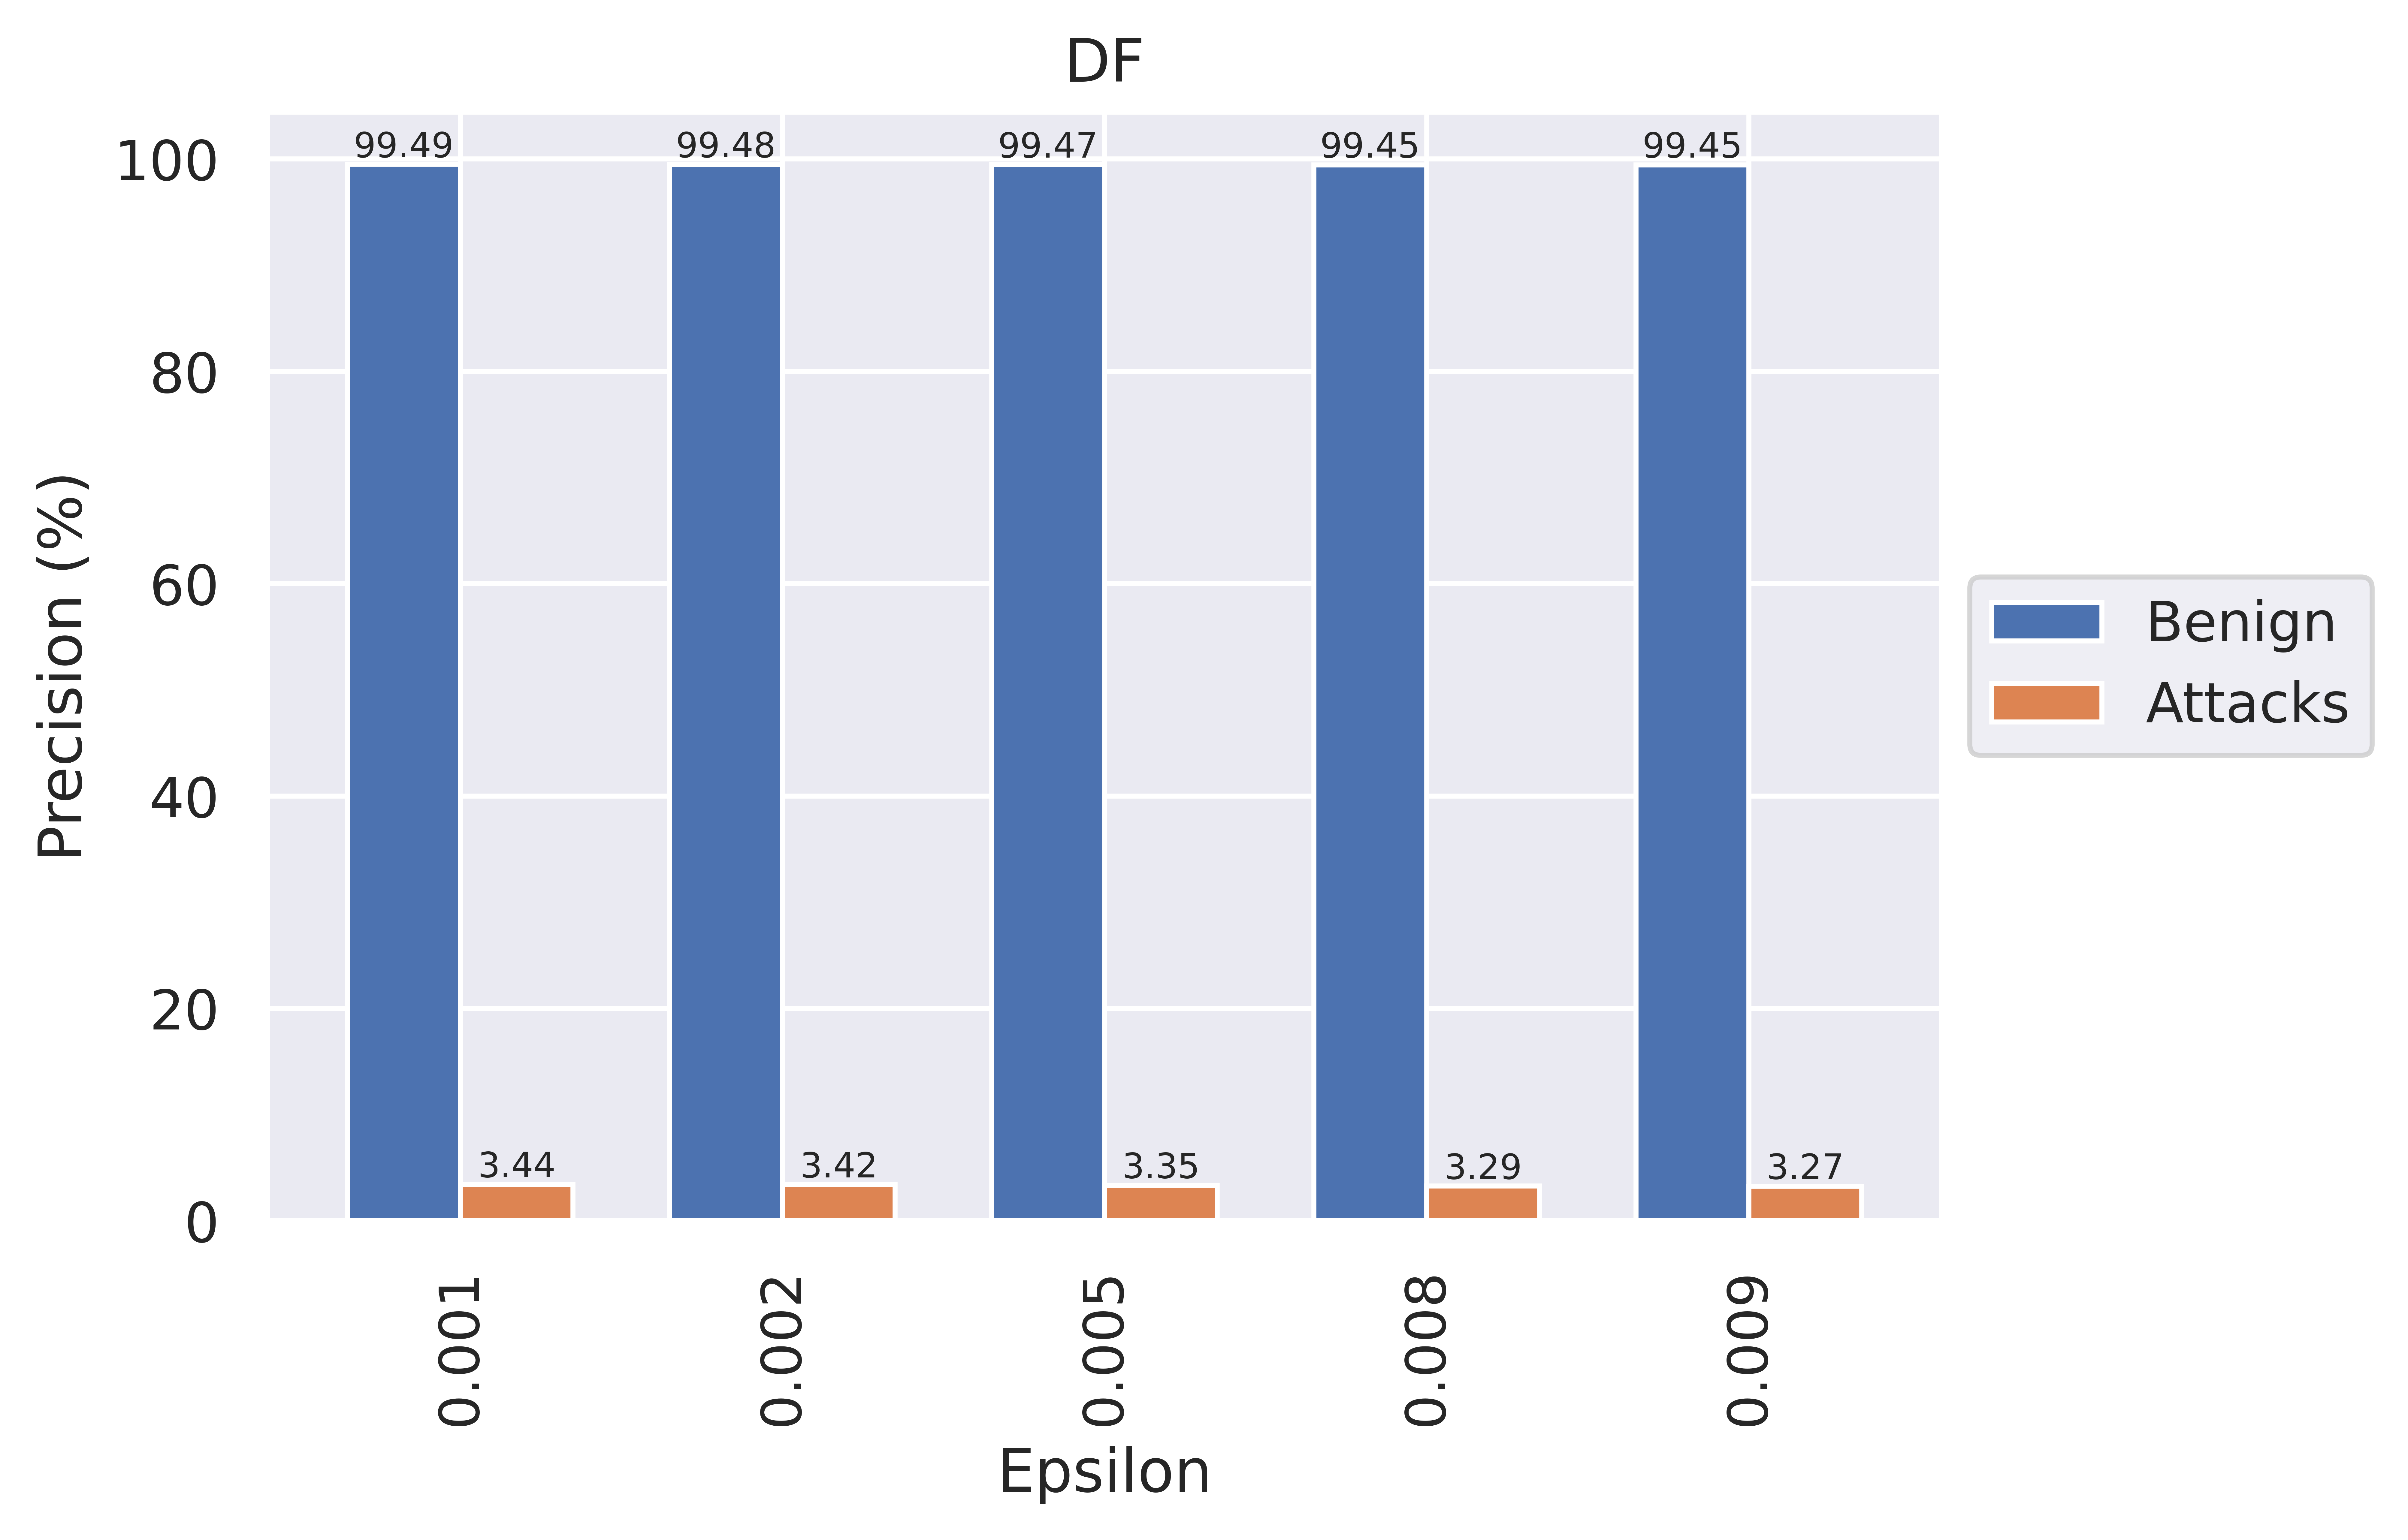
\includegraphics[width=\textwidth]{/home/wojtyla/Documentos/Artigo_2023/IJCNN_Suplementary/Figures//UNSW_Clean_DF_bin_paper.png}
			%caption{Figure}
			\label{fig:1}
		\end{subfigure}
		\hfill
		\begin{subfigure}[b]{0.45\textwidth}
			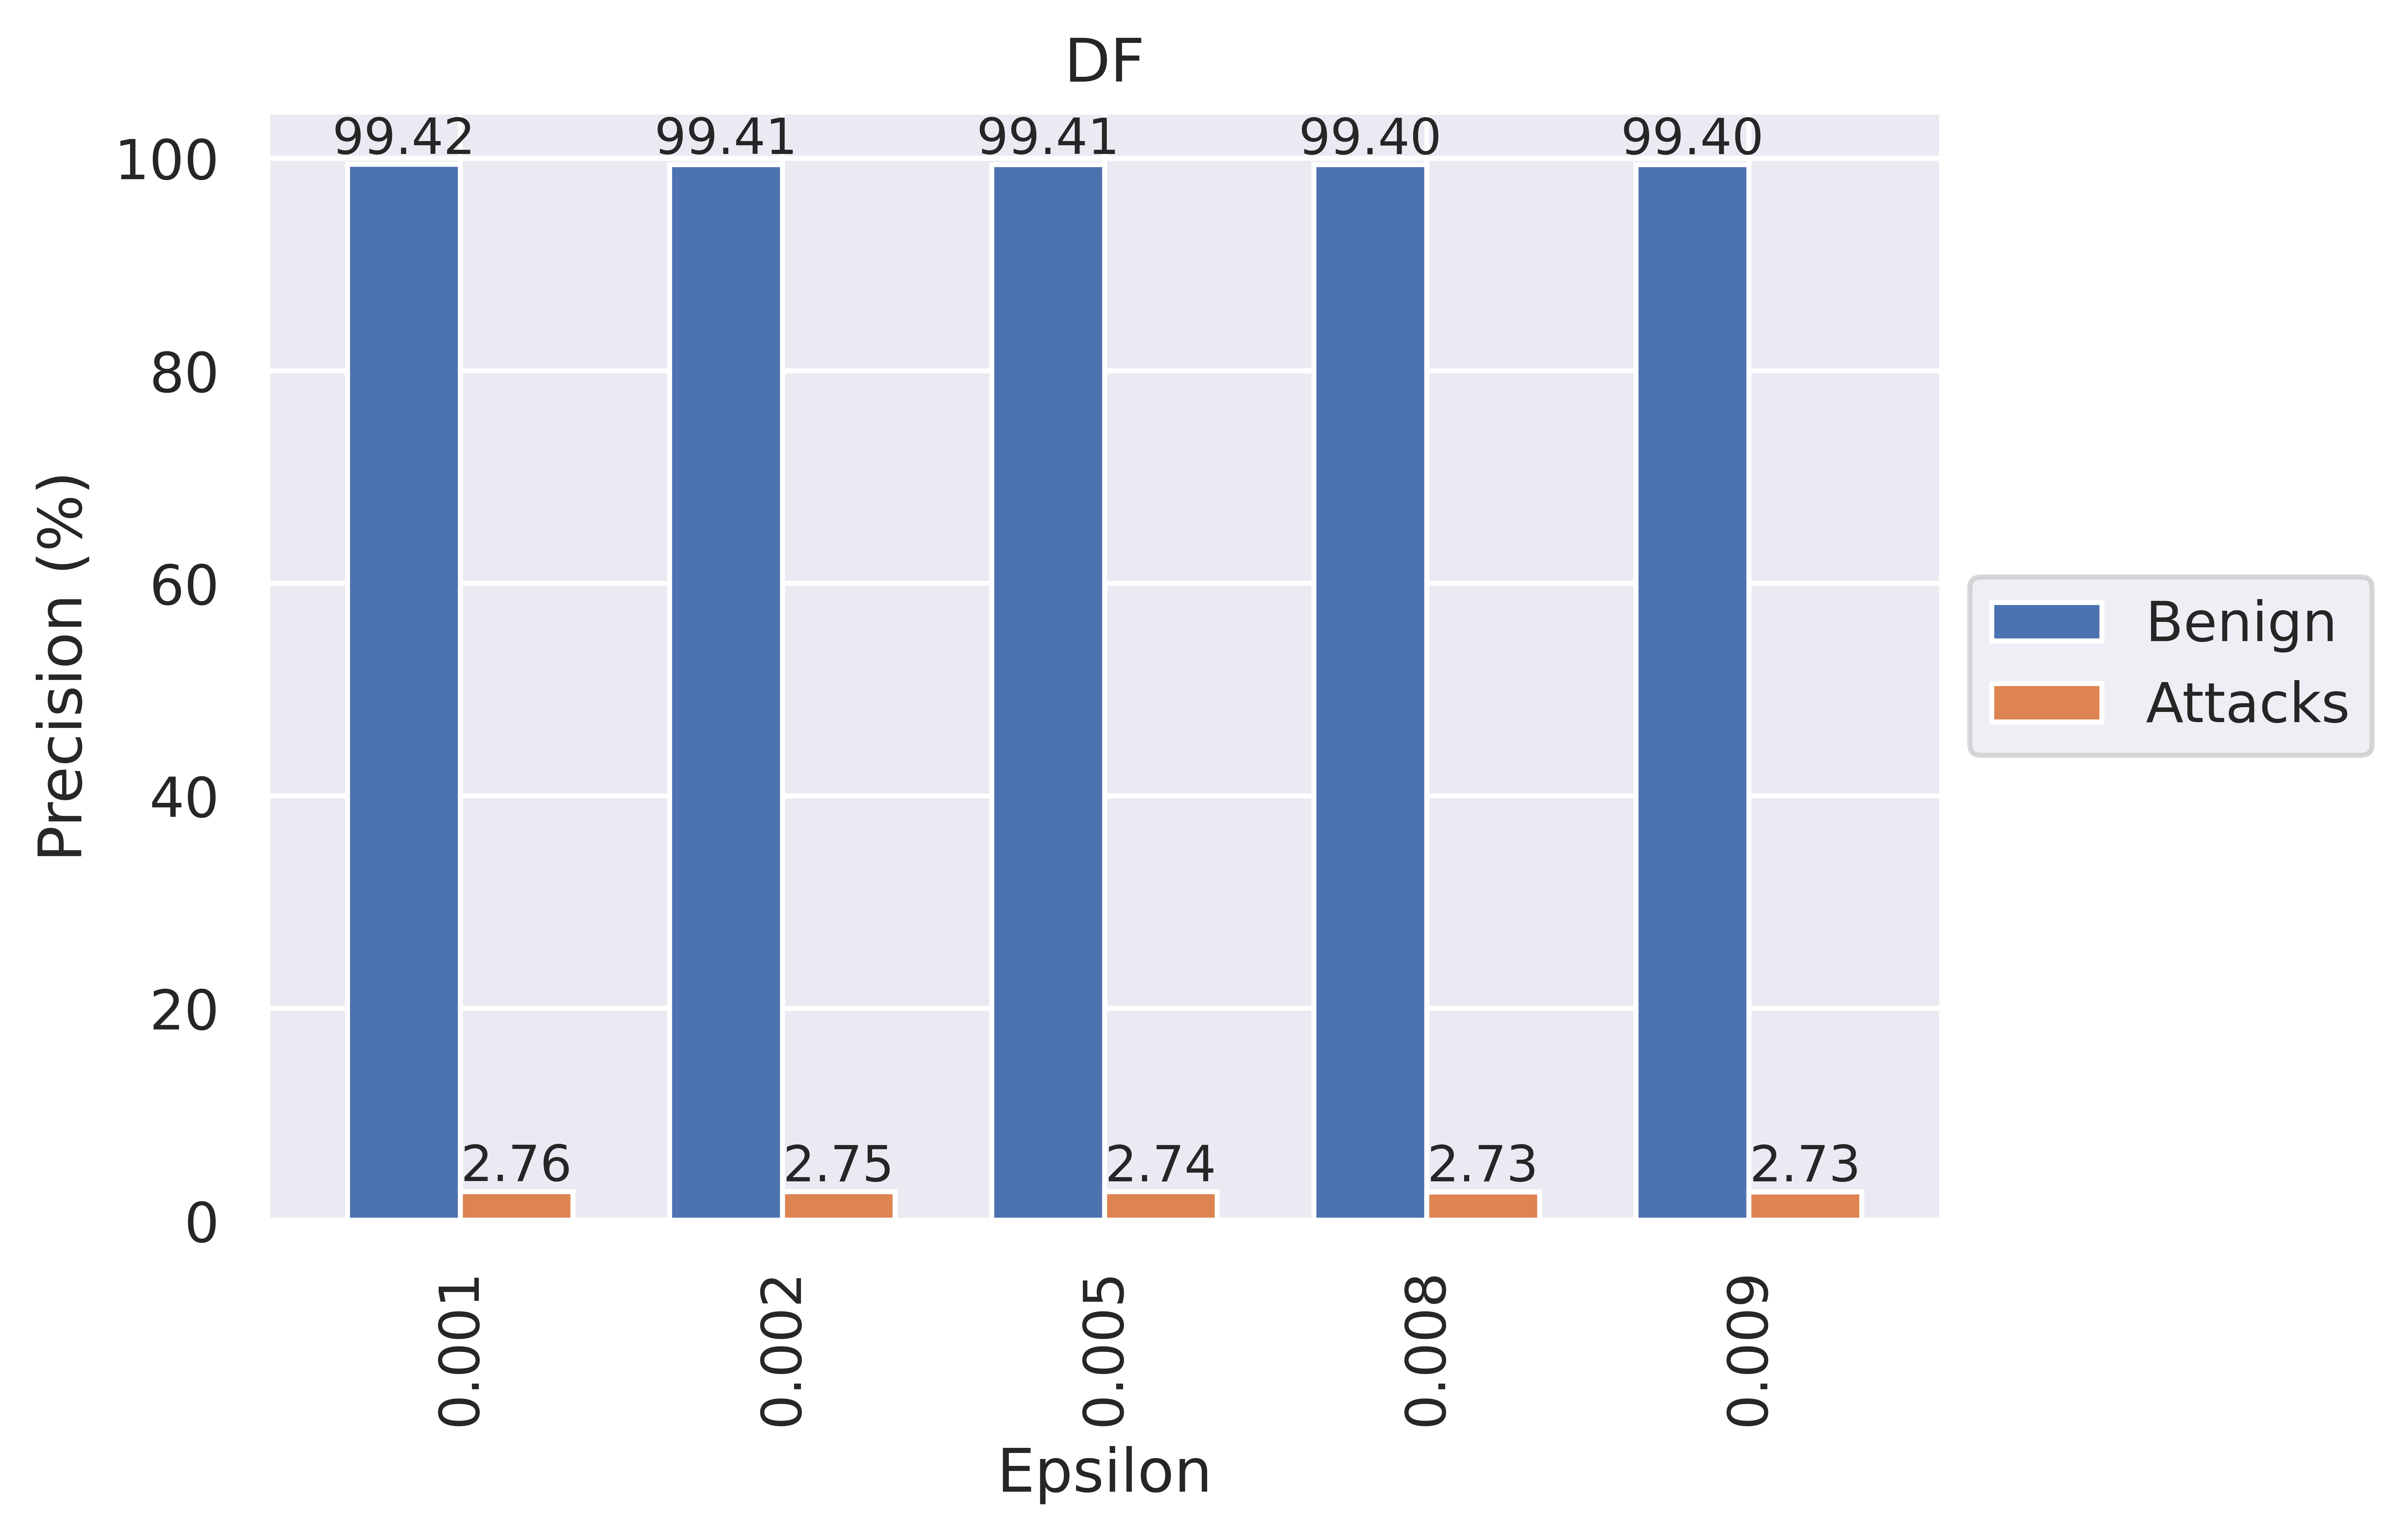
\includegraphics[width=\textwidth]{/home/wojtyla/Documentos/Artigo_2023/IJCNN_Suplementary/Figures//UNSW_IDS_DF_bin_paper.png}
			%caption{Figure}
			\label{fig:4}
		\end{subfigure}
		\caption{Plots for DF-2 attack on binary models with UNSW-NB15.Left:EnC model; Right:EnIDS model.}
		\label{fig:unsw_df_bin}
	\end{figure}
	
	
	
	\begin{table}[H]
		\caption{DF-2 attack against EnC and EnIDS for multiclass classification on the UNSW-NB15 dataset.}
		\small
		\setlength{\tabcolsep}{0.1pt}
		\centering
		\label{tab:unsw_multi_df}
		\hspace*{-1.6cm}
		\begin{adjustbox}{width=1.2\textwidth}
			\begin{tabular}{|c|c|c|c|c|c|c|c|c|c|c|c|c|c|c|c|c|}
				\hline
				\multirow{4}{*}{\textbf{Type}} & \multirow{4}{*}{\textbf{Metric}}& \multicolumn{15}{c|}{\textbf{Epsilon ($\epsilon$)}} \\
				\cline{3-17}
				&  & \multicolumn{3}{c|}{\textbf{0.001}} & \multicolumn{3}{c|}{\textbf{0.002}} & \multicolumn{3}{c|}{\textbf{0.005}} & \multicolumn{3}{c|}{\textbf{0.008}} & \multicolumn{3}{c|}{\textbf{0.009}} 
				\\
				\cline{3-17}
				&  & \textbf{\textsl{Normal}} & \textbf{\textsl{Recon.}} & \textbf{\textsl{Generic}} & \textbf{\textsl{Normal}} & \textbf{\textsl{Recon.}} & \textbf{\textsl{Generic}} & \textbf{\textsl{Normal}} & \textbf{\textsl{Recon.}} & \textbf{\textsl{Generic}} & \textbf{\textsl{Normal}} & \textbf{\textsl{Recon.}} & \textbf{\textsl{Generic}} & \textbf{\textsl{Normal}} & \textbf{\textsl{Recon.}} & \textbf{\textsl{Generic}}
				\\
				\hline
				\multirow{3}{*}{EnC} & Precision & 100.00 & 60.98 & 95.42 & 100.00 & 60.73 & 95.40 & 100.00 & 60.98 & 95.36 & 100.00 & 60.98 & 95.32 & 100.00 & 60.98 & 95.30
				\\
				
				& Recall & 99.42 & 42.61 & 63.70 & 99.40 & 42.61 & 63.43 & 99.33 & 42.61 & 62.90 & 99.24 & 42.61 & 62.23 & 99.20 & 42.61 & 62.03
				\\
				
				& ROC-AUC & 99.93 & 99.78 & 99.90 & 99.93 & 99.78 & 99.90 & 99.93 & 99.77 & 99.89 & 99.91 & 99.77 & 99.89 & 99.91 & 99.77 & 99.89
				\\
				\hline
				\multirow{3}{*}{EnIDS} & Precision & \cellcolor{blue!20}100.00 & 17.92 & 66.02 & \cellcolor{blue!20}100.00 & 17.95 & 66.02 & \cellcolor{blue!20}100.00 & 17.95 & 65.73 & \cellcolor{blue!20}100.00 & 17.90 & 66.89 & \cellcolor{blue!20}100.00 & 17.87 & 66.89
				\\
				
				& Recall & 86.21 & 32.39 & 20.28 & 86.20 & 32.39 & 20.28 & 86.13 & 32.39 & 20.15 & 86.07 & 32.39 & 20.28 & 86.05 & 32.39 & 20.28
				\\
				
				& ROC-AUC & 98.14 & 99.47 & 99.34 & 98.13 & 99.47 & 99.34 & 98.11 & 99.46 & 99.33 & 98.09 & 99.46 & 99.33 & 98.08 & 99.46 & 99.33
				\\
				\hline
			\end{tabular}	
		\end{adjustbox}	
	\end{table}
	
	\begin{figure}[H]
		\centering
		\begin{subfigure}[b]{0.45\textwidth}
			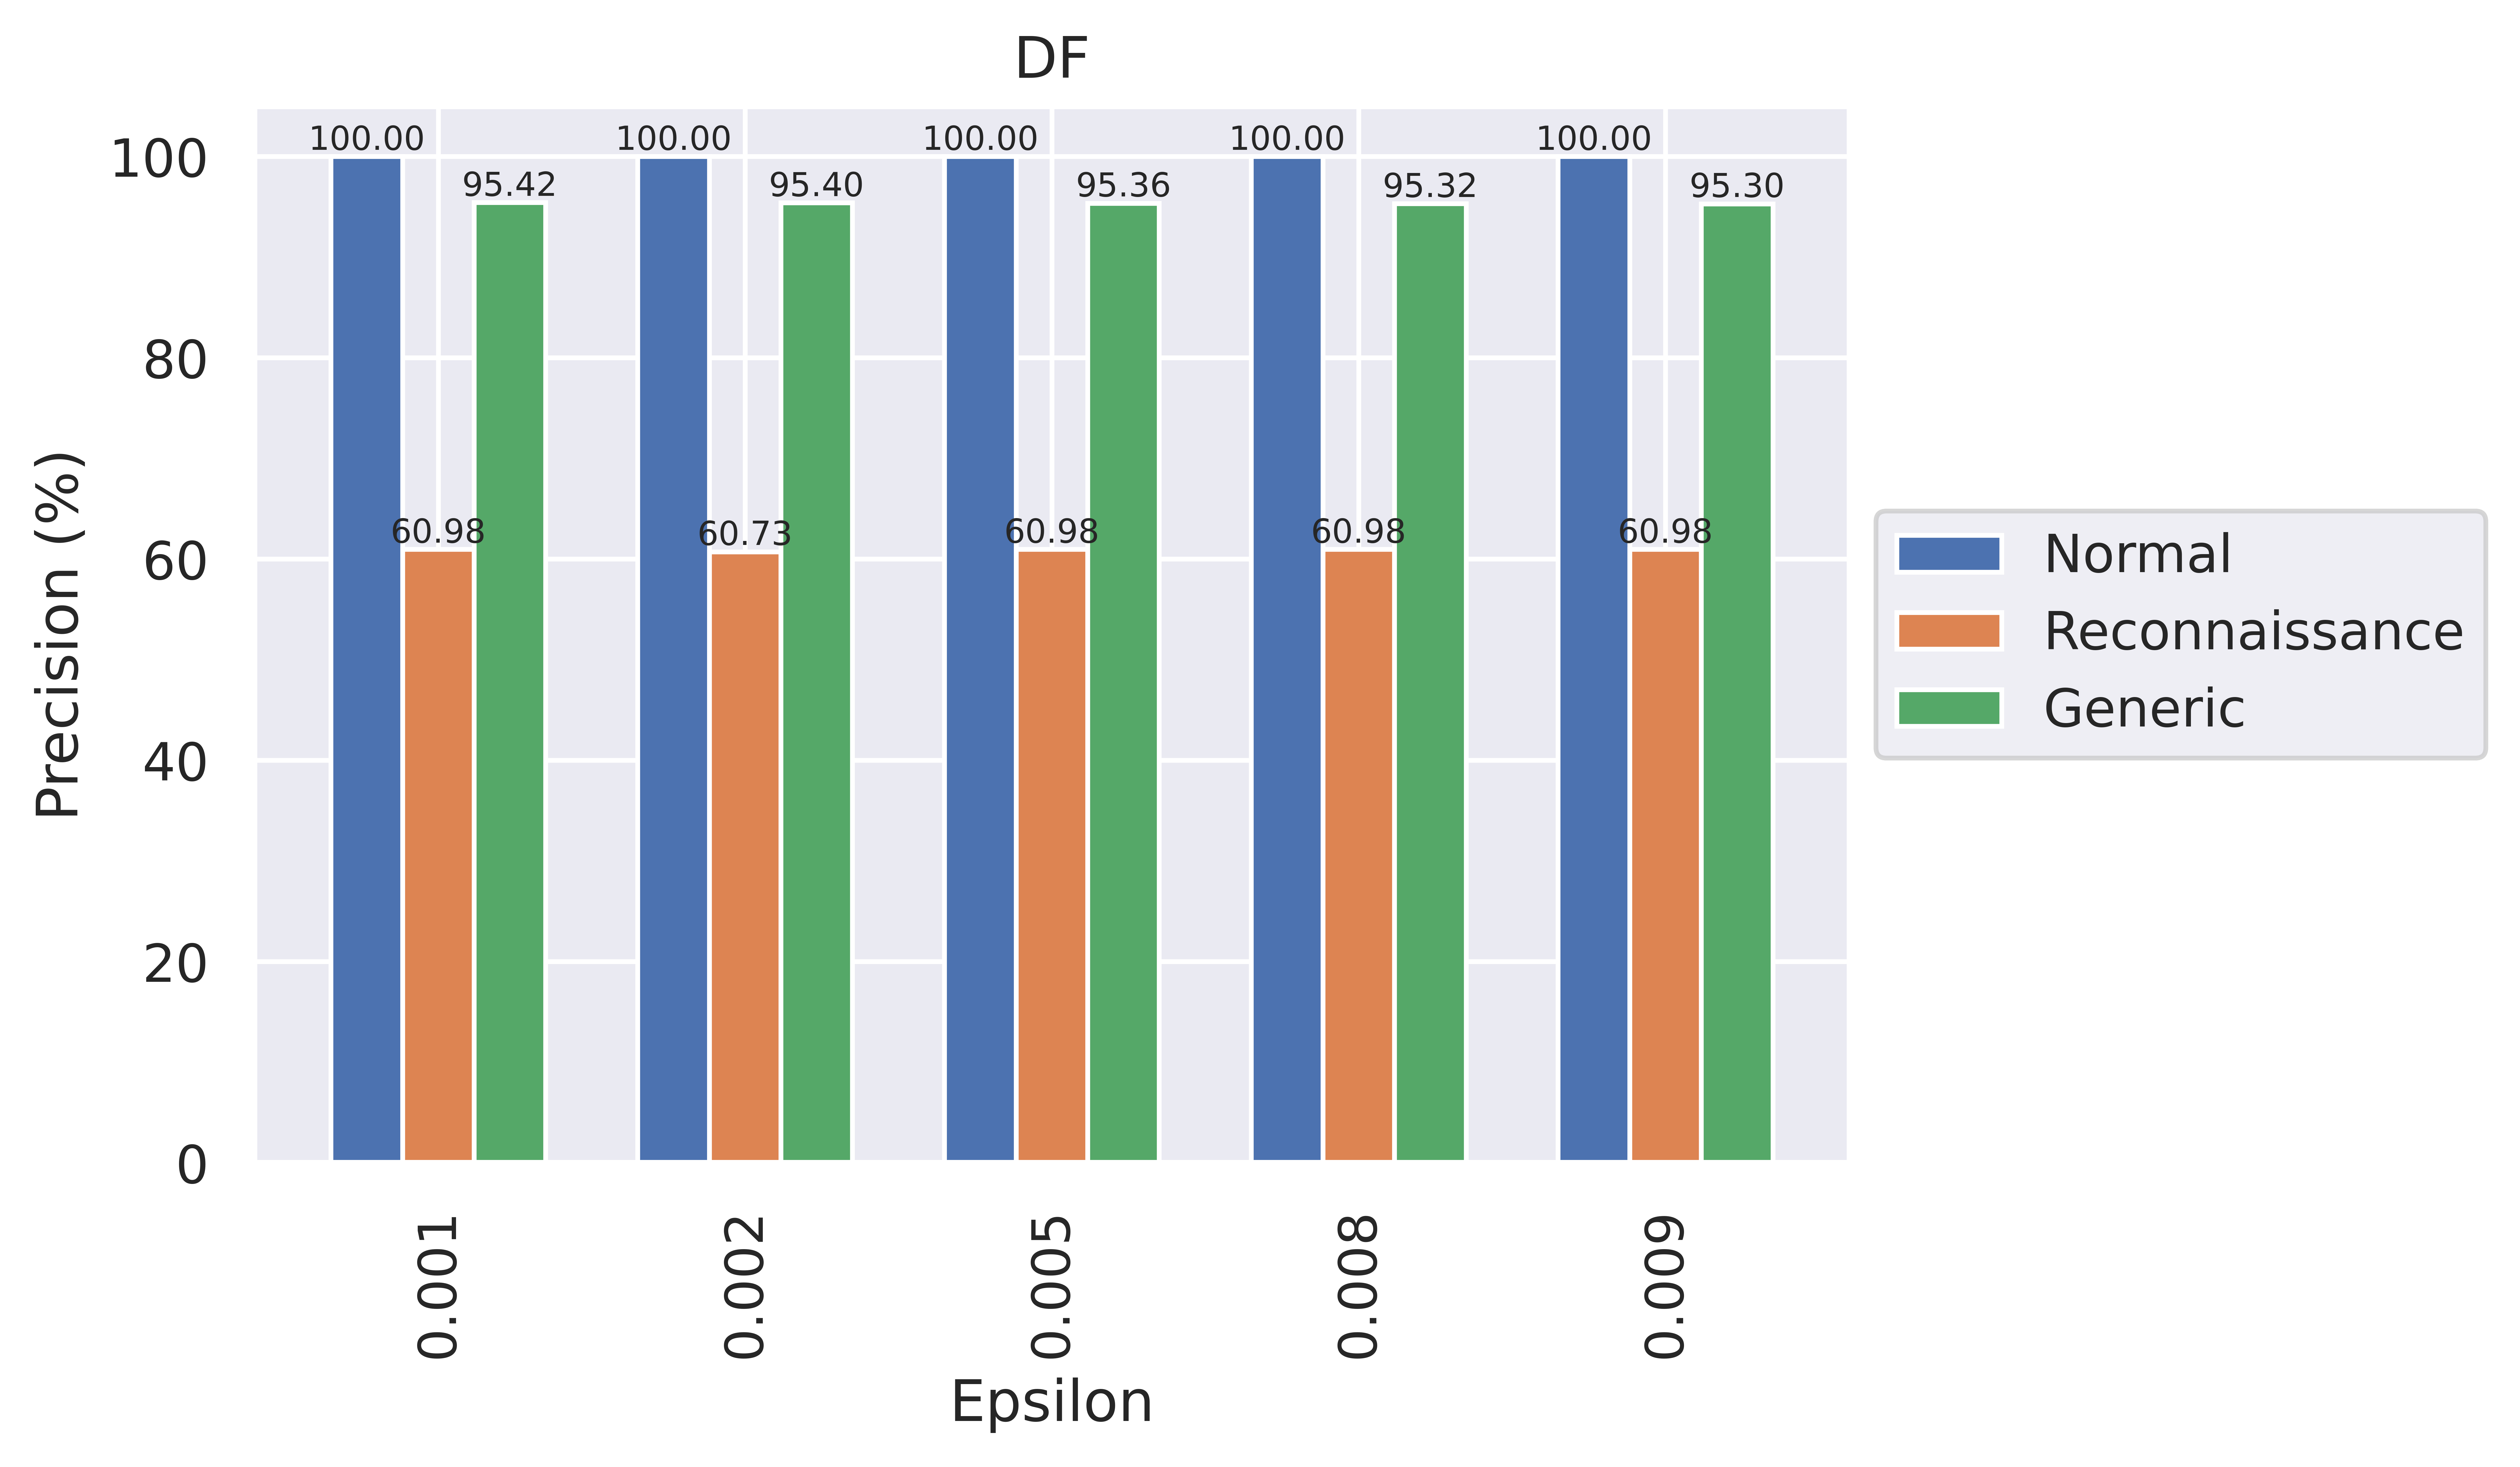
\includegraphics[width=\textwidth]{/home/wojtyla/Documentos/Artigo_2023/IJCNN_Suplementary/Figures/UNSW_Clean_DF_multi_paper.png}
			%caption{Figure}
			\label{fig:1}
		\end{subfigure}
		\hfill
		\begin{subfigure}[b]{0.45\textwidth}
			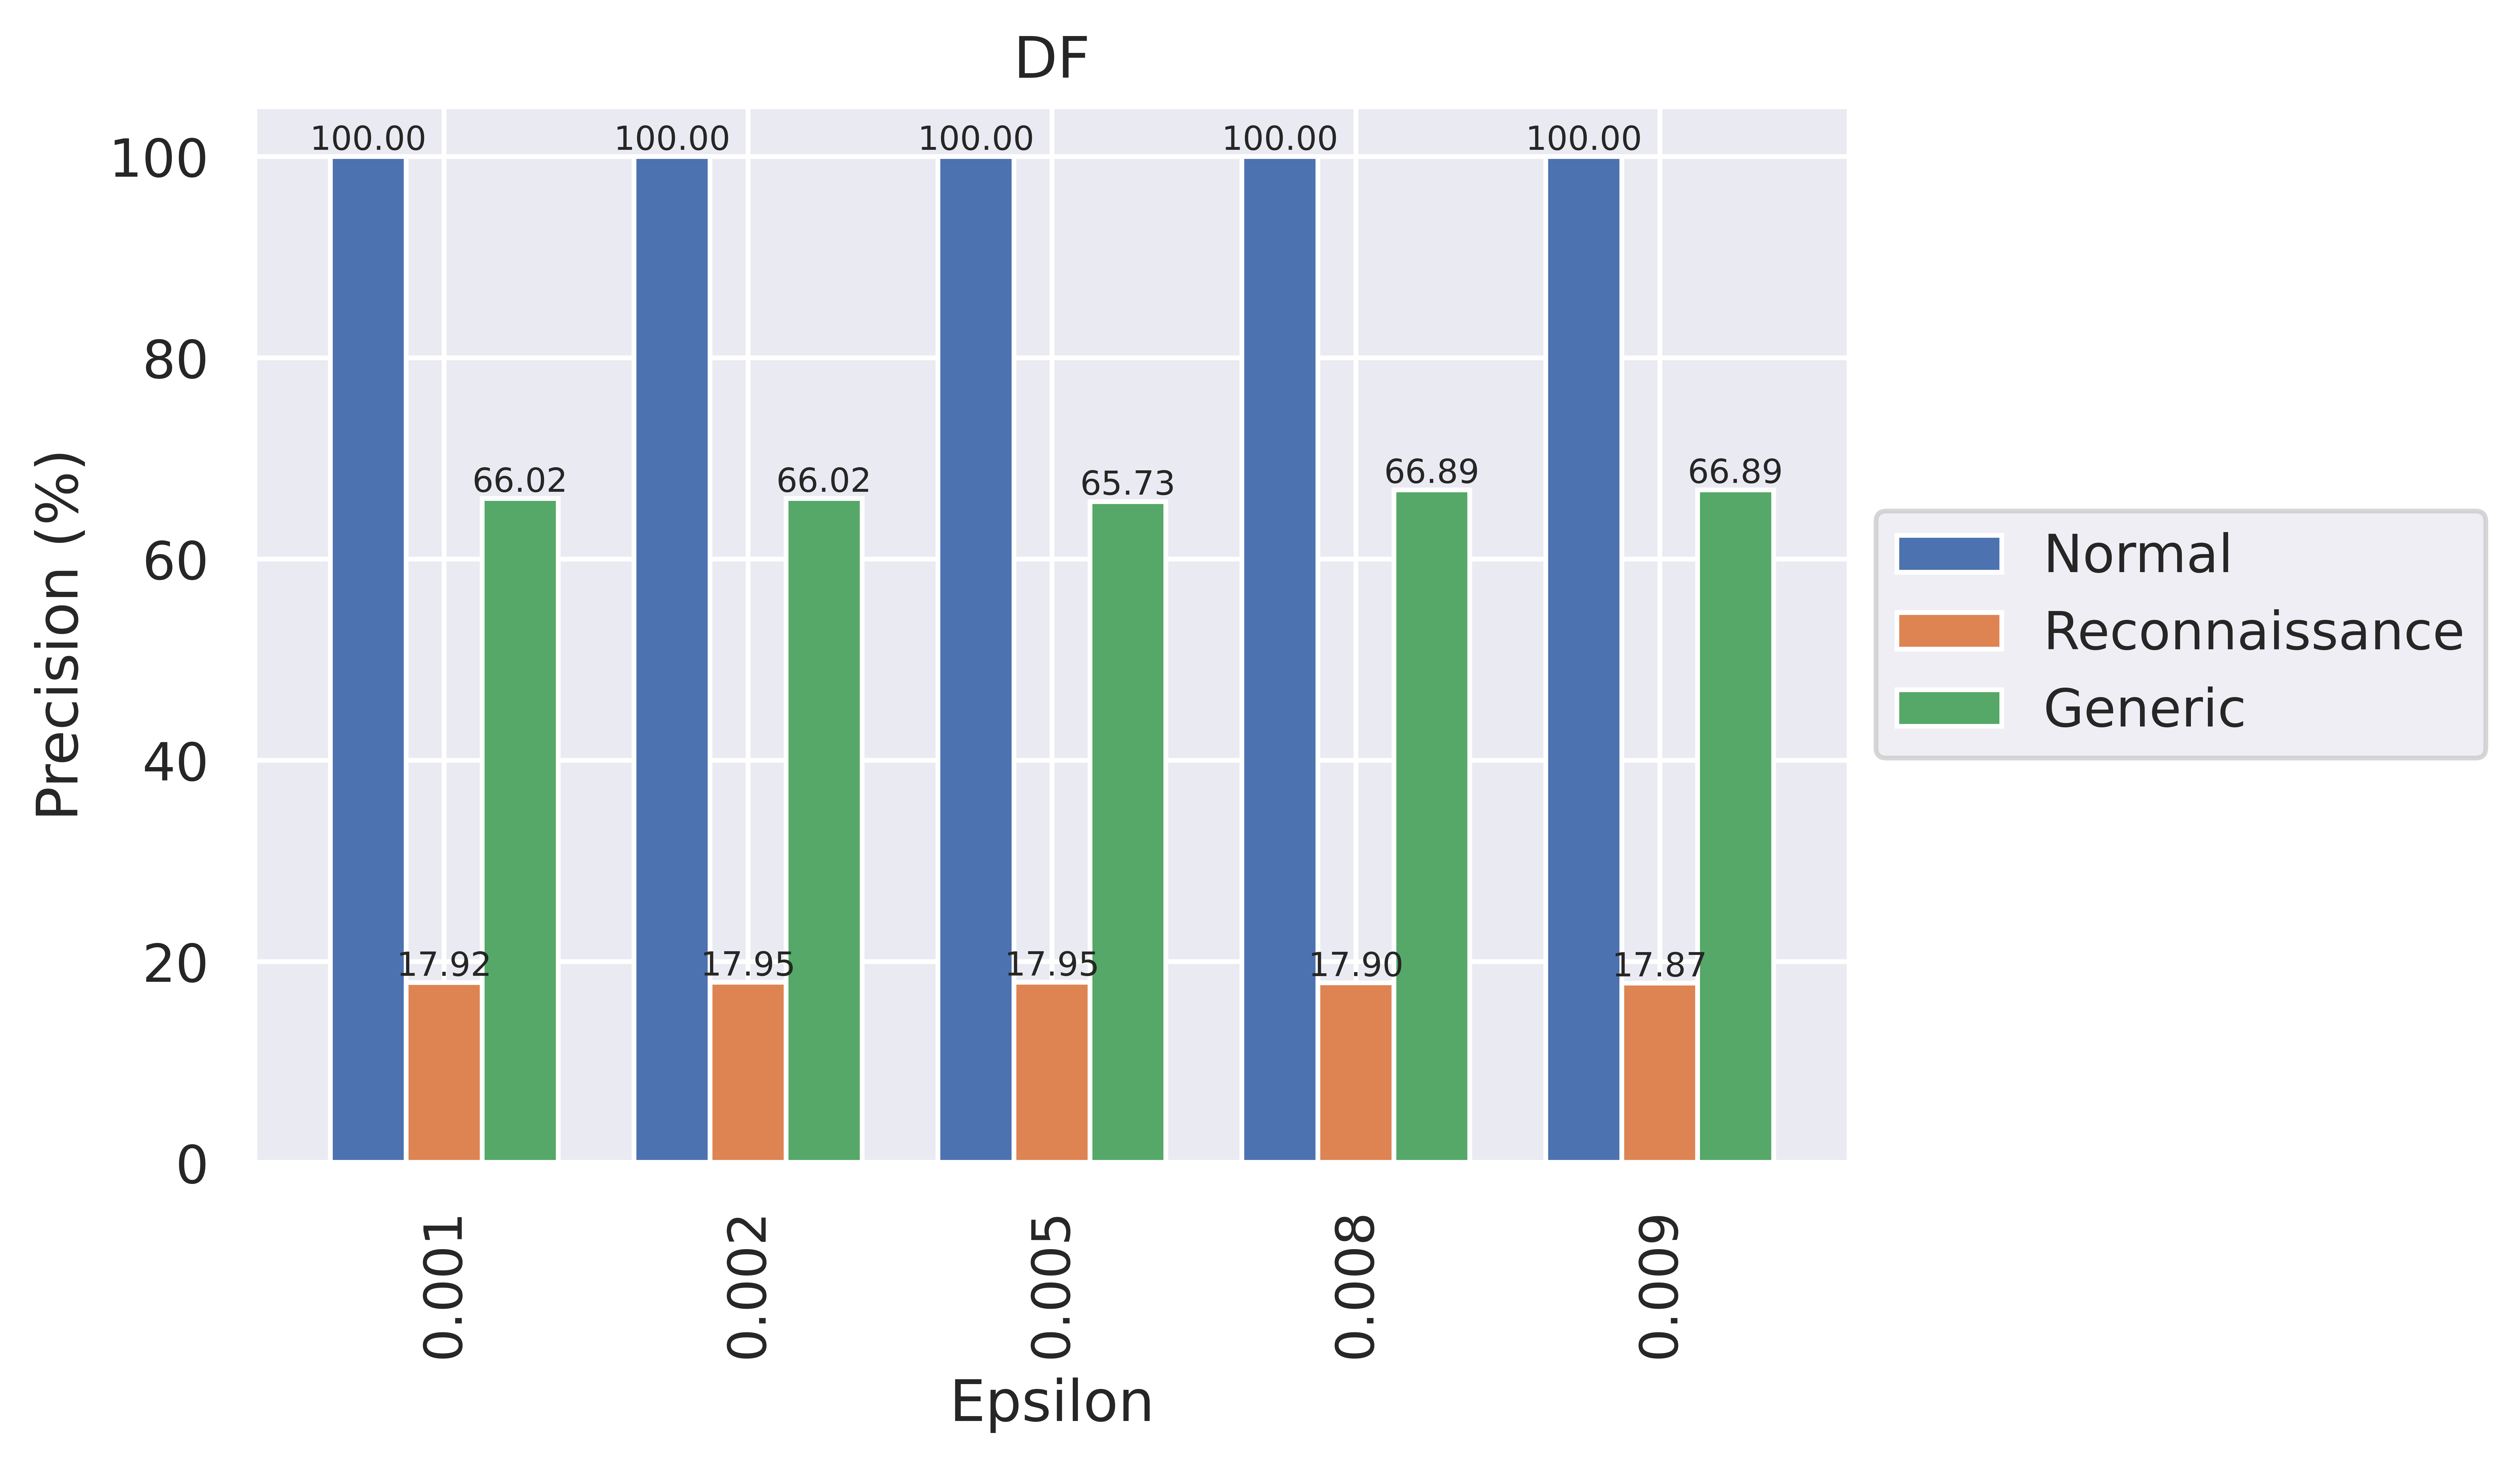
\includegraphics[width=\textwidth]{/home/wojtyla/Documentos/Artigo_2023/IJCNN_Suplementary/Figures/UNSW_IDS_DF_multi_paper.png}
			%caption{Figure}
			\label{fig:4}
		\end{subfigure}
		\caption{Plots for DF-2 attack on multiclass models with UNSW-NB15.Left:EnC model; Right:EnIDS model.}
		\label{fig:unsw_df_multi}
	\end{figure}
	
	
	\section{Boundary, HopSkipJump, SignOPT}
	
	\subsection{CIC IDS2017}
	
	\begin{table}[H]
		\caption{Black-Box attacks against EnC and EnIDS for binary classification on the CIC IDS2017 dataset.}
		\small
		\setlength{\tabcolsep}{0.1pt}
		\centering
		\label{tab:cic_bin_black}
		
		\begin{tabular}{|c|c|c|c|c|}
			\hline
			\multirow{2}{*}{\textbf{Type}} & \multirow{2}{*}{\textbf{Attacks}} & \multirow{2}{*}{\textbf{Metrics}} &  \multicolumn{2}{c|}{\textbf{Label}} \\
			\cline{4-5}
			&  &  & \textbf{Benign} & \textbf{Attacks} \\
			\hline
			\multirow{9}{*}{EnC} & 	\multirow{3}{*}{Boundary} & Precision & 83.02 & 16.83 \\
			
			&  & Recall & 67.71 & 32.07 \\
			
			&  & ROC-AUC & 52.23 & 58.04 \\
			\cline{2-5}
			& \multirow{3}{*}{HopSkipJump} & Precision & 83.02 & 16.82 \\
			
			&  & Recall & 67.81 & 31.93 \\
			
			&  & ROC-AUC & 73.71 & 73.92 \\
			\cline{2-5}
			& \multirow{3}{*}{SignOPT} & Precision & 85.73 & 22.51 \\
			
			&  & Recall & 69.88 & 42.93 \\
			
			&  & ROC-AUC & 80.60 & 81.02 \\
			\hline
			\multirow{9}{*}{EnIDS} & \multirow{3}{*}{Boundary} & Precision & \cellcolor{yellow!50}83.10 & 17.09 \\
			
			&  & Recall & \cellcolor{yellow!50}83.88 & 16.30 \\
			
			&  & ROC-AUC & \cellcolor{yellow!50}82.08 & \cellcolor{yellow!50}83.52 \\
			\cline{2-5}
			& \multirow{3}{*}{HopSkipJump} & Precision & \cellcolor{yellow!50}83.10 & 17.07 \\
			
			&  & Recall & \cellcolor{yellow!50}83.80 & 16.36 \\
			
			&  & ROC-AUC & \cellcolor{yellow!50}86.37 & \cellcolor{yellow!50}86.38 \\
			\cline{2-5}
			& \multirow{3}{*}{SignOPT} & Precision & \cellcolor{yellow!50}86.98 & 40.52 \\
			
			&  & Recall & \cellcolor{yellow!50}89.82 & 34.01 \\
			
			&  & ROC-AUC & \cellcolor{yellow!50}93.21 & \cellcolor{yellow!50}93.22 \\
			\hline
		\end{tabular}			
	\end{table}
	
	\begin{figure}[H]
		\centering
		\begin{subfigure}[b]{0.3\textwidth}
			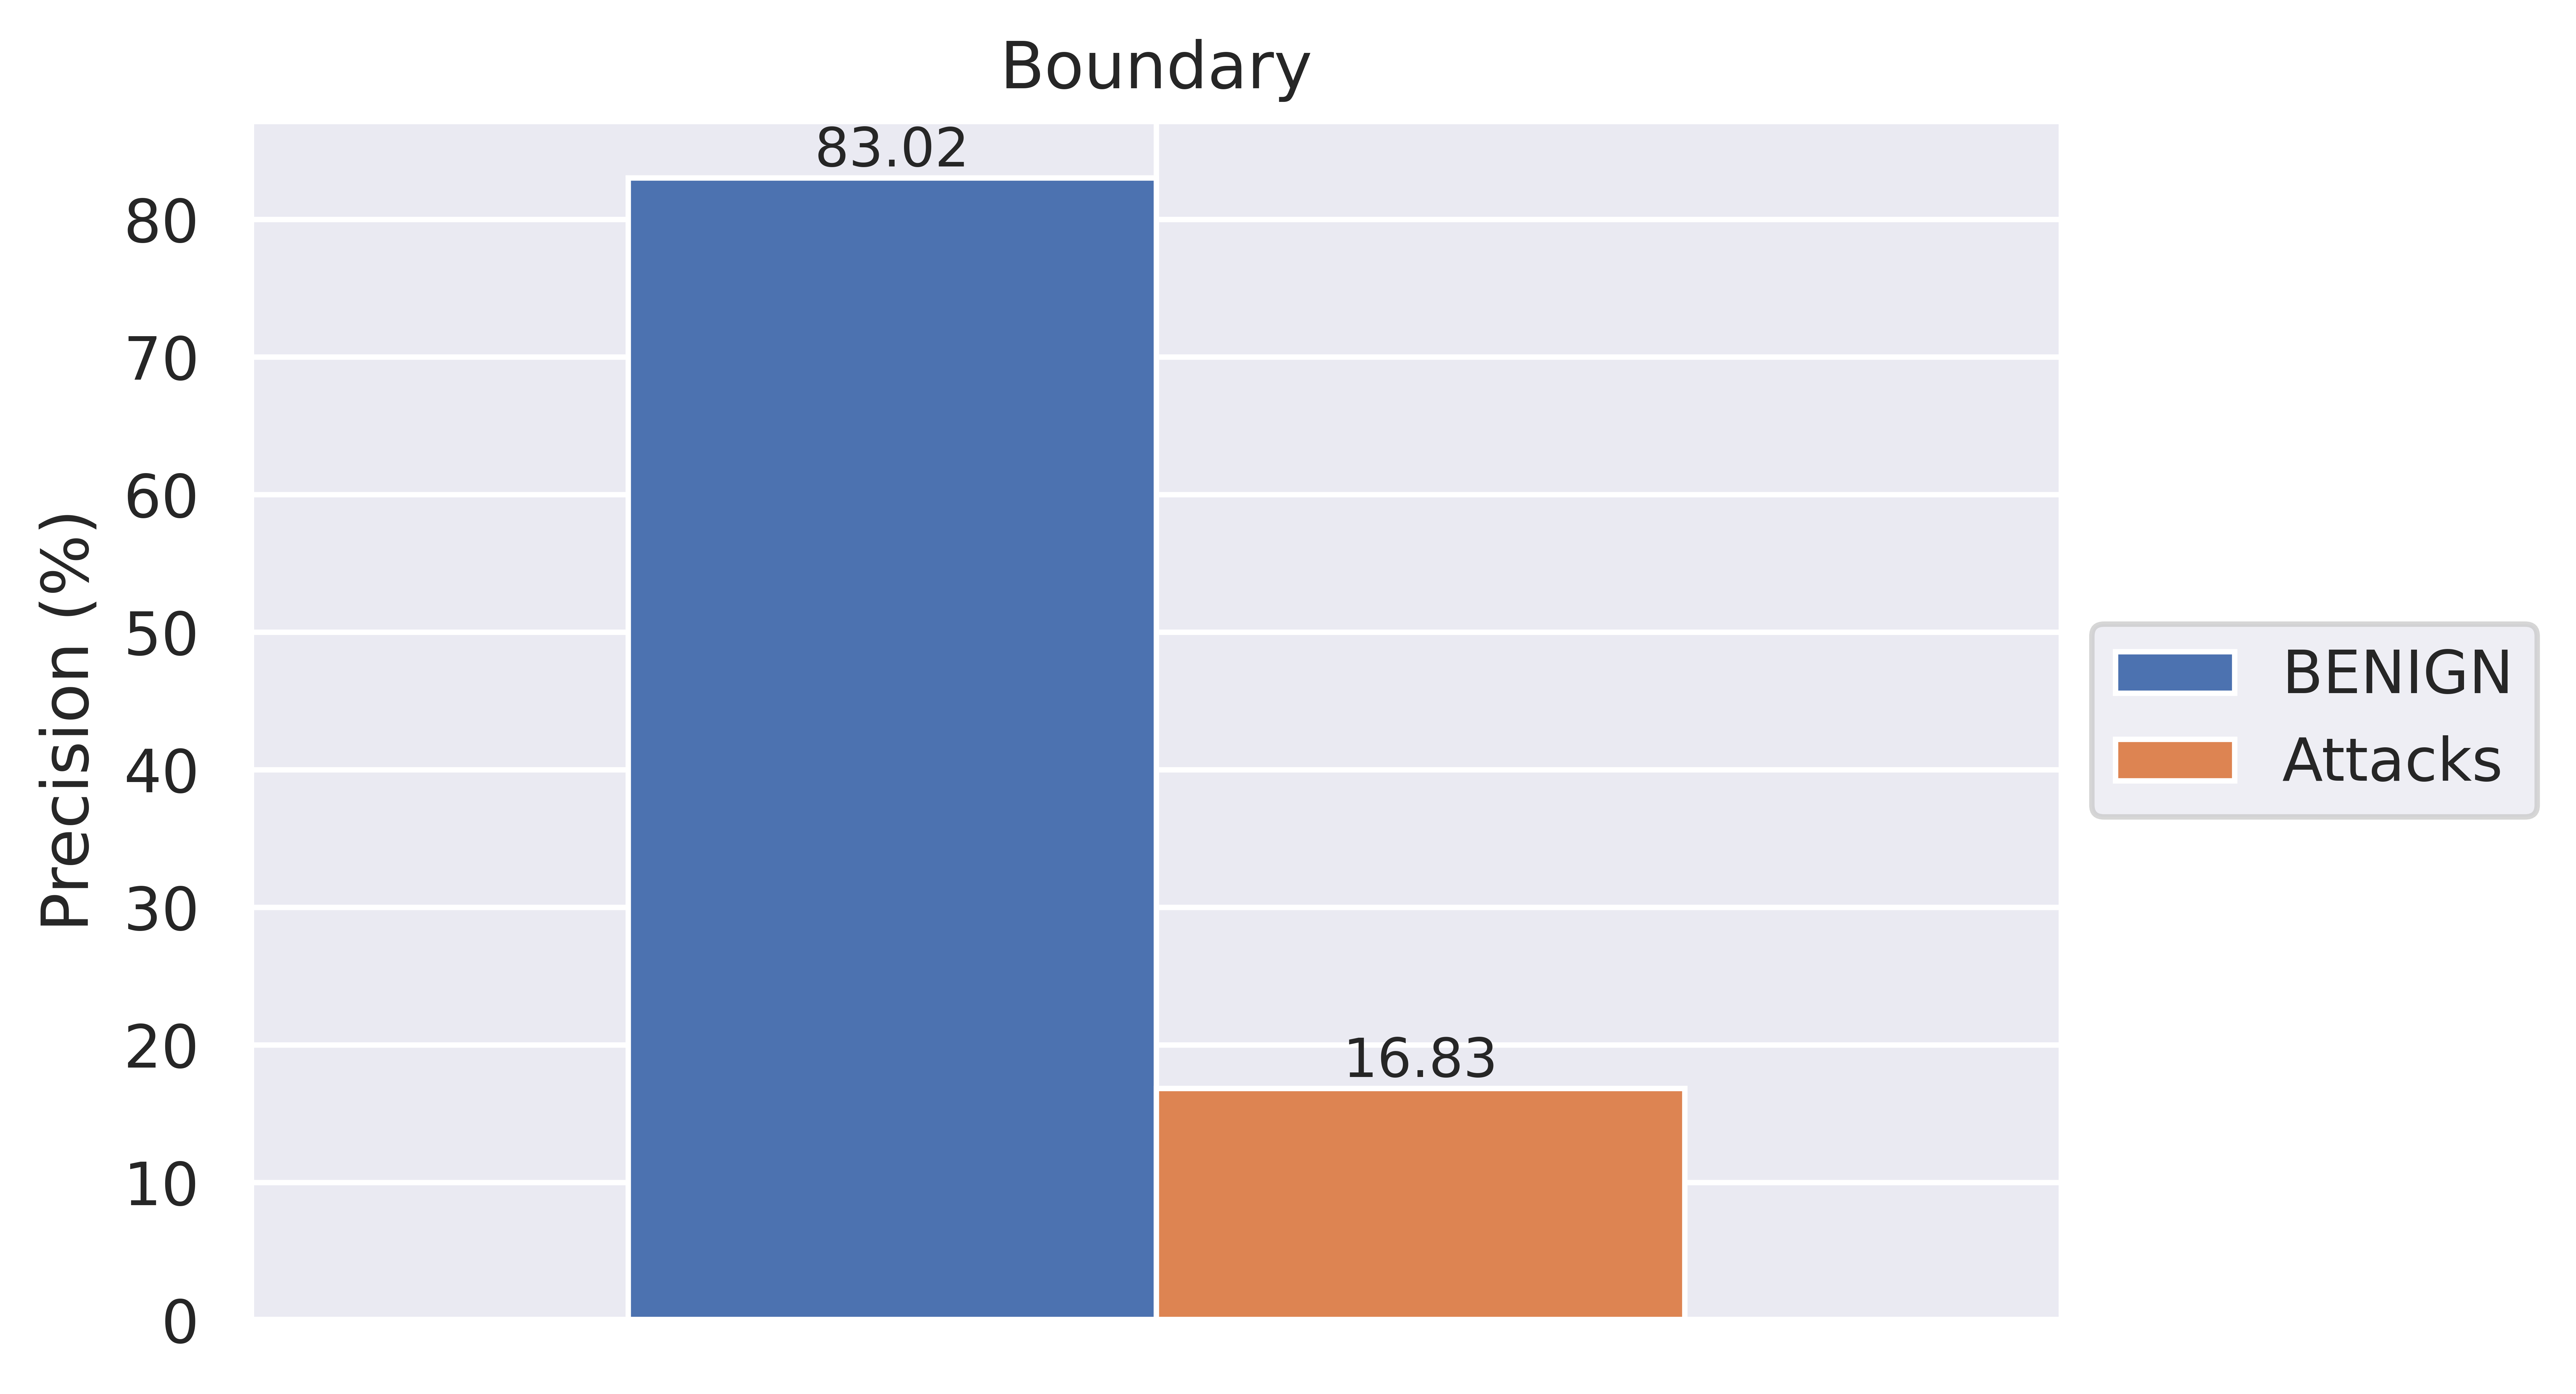
\includegraphics[width=\textwidth]{/home/wojtyla/Documentos/Artigo_2023/IJCNN_Suplementary/Figures//CIC_Clean_Boundary_bin_paper.png}
			%caption{Figure}
			\label{fig:1}
		\end{subfigure}
		\hfill
		\begin{subfigure}[b]{0.3\textwidth}
			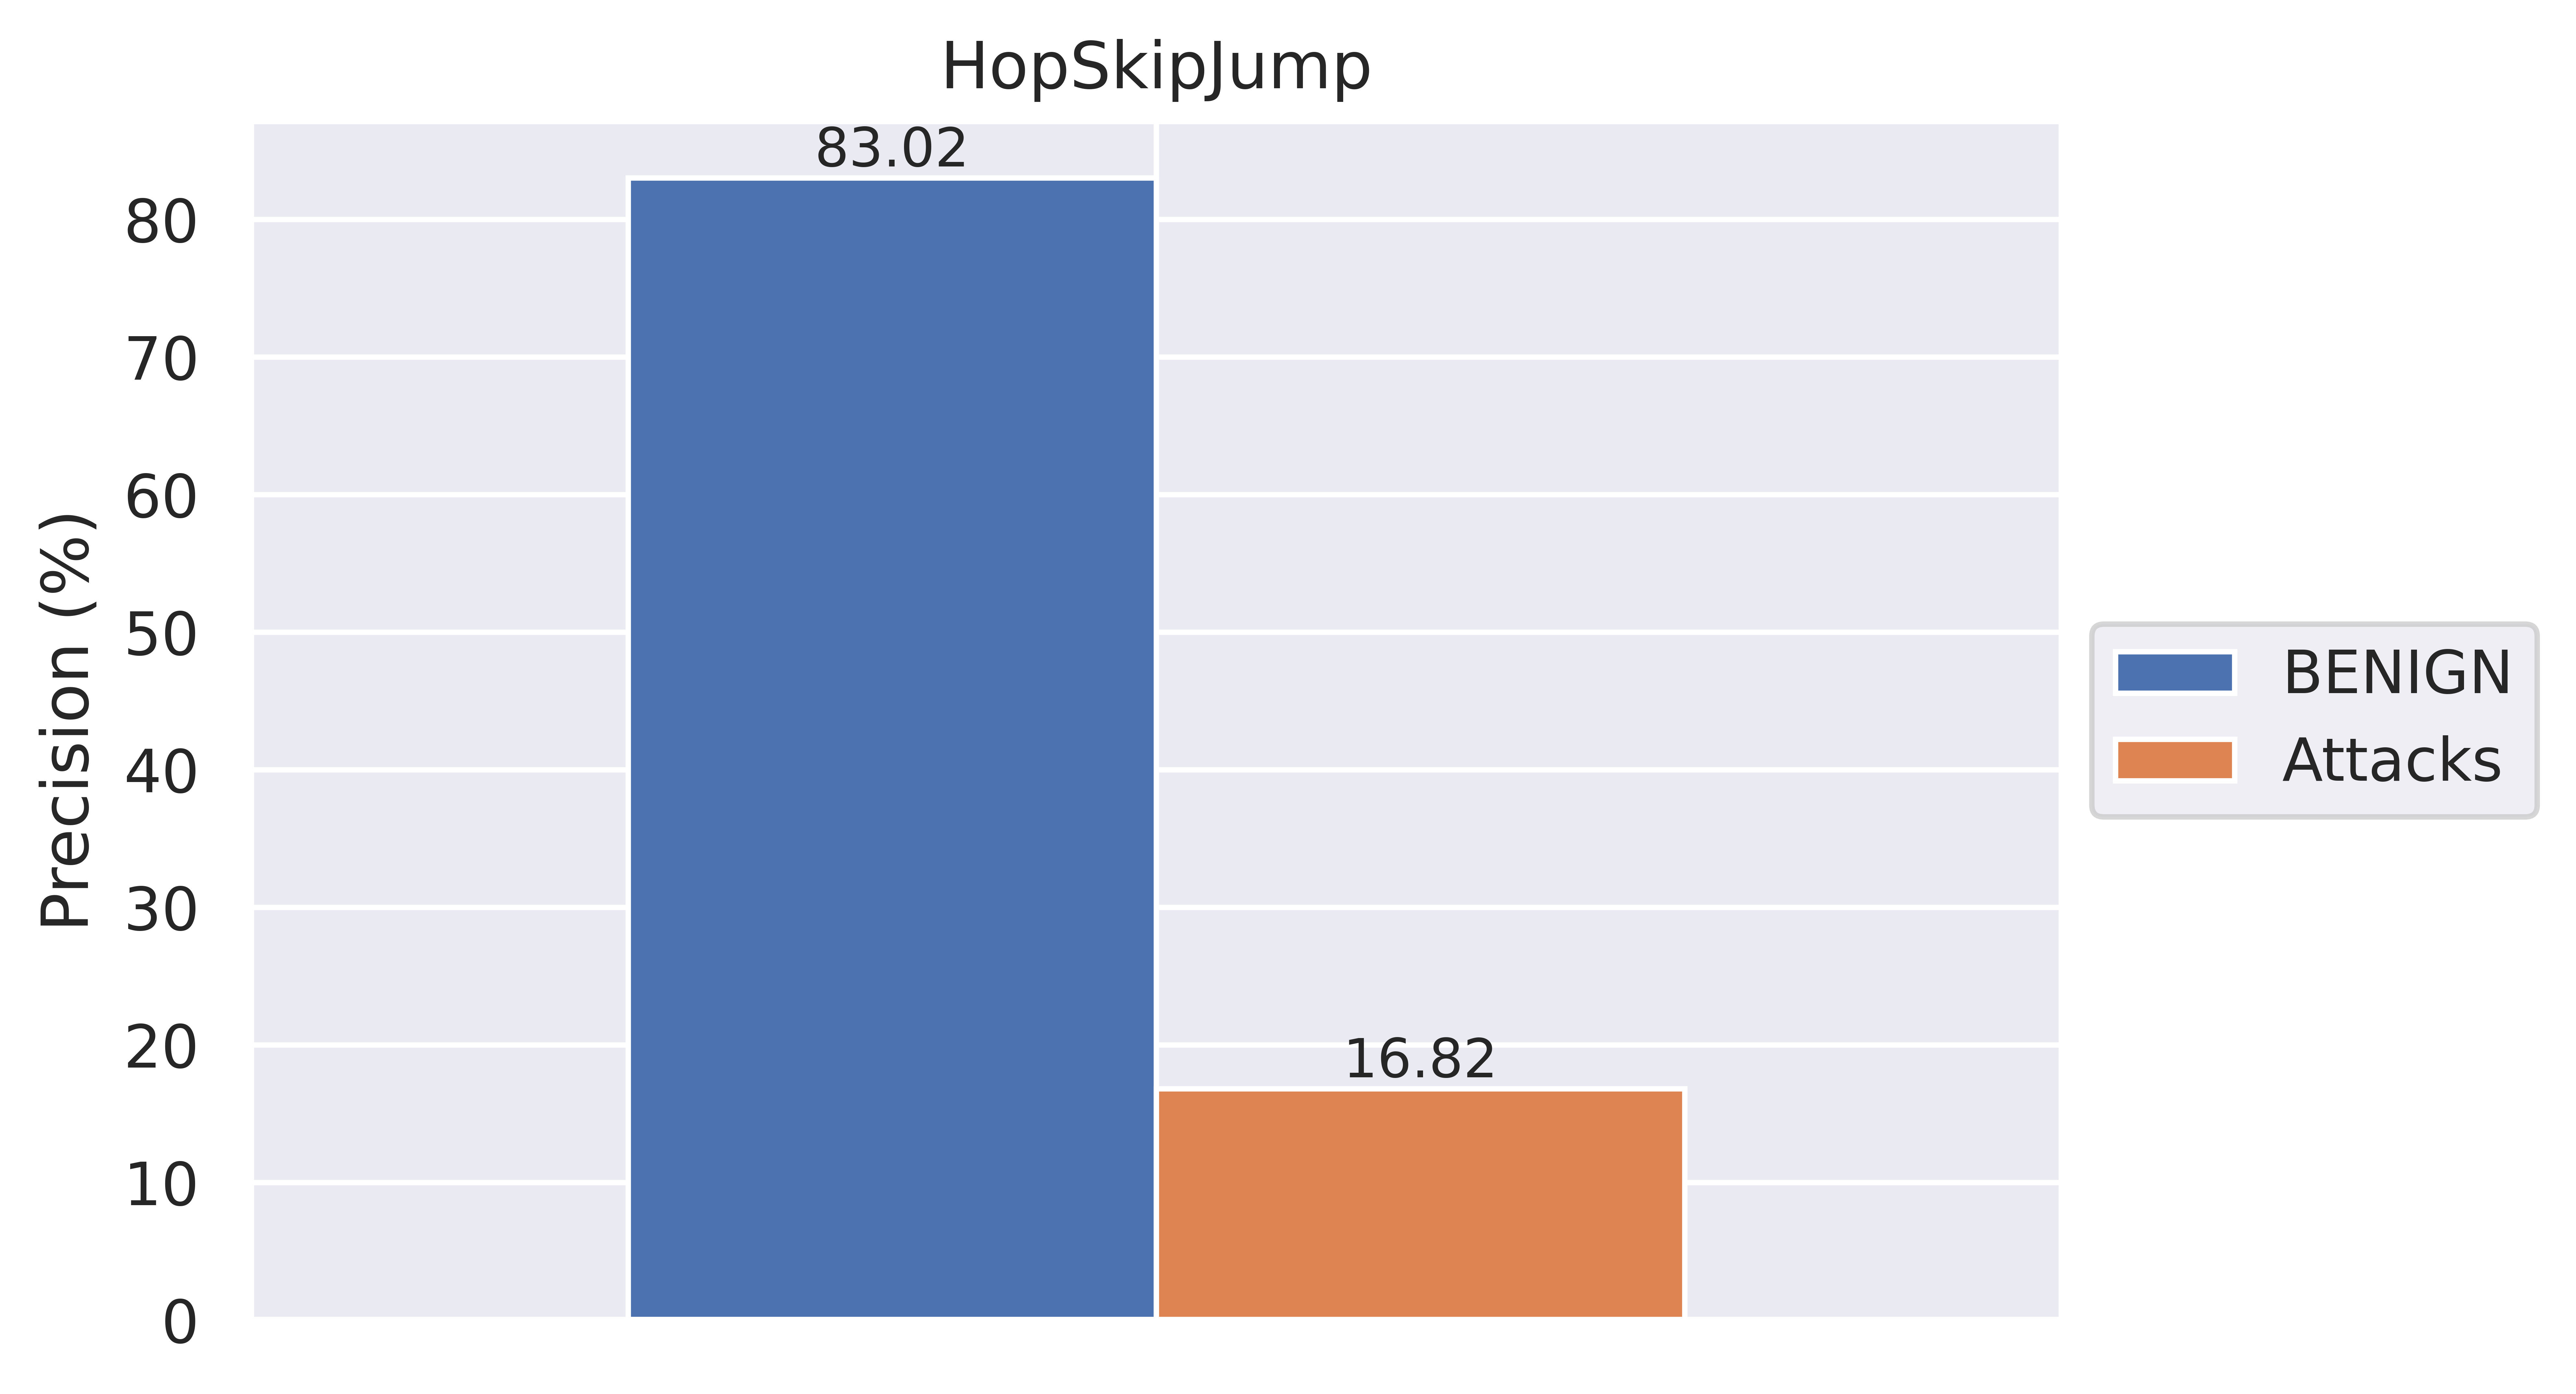
\includegraphics[width=\textwidth]{/home/wojtyla/Documentos/Artigo_2023/IJCNN_Suplementary/Figures//CIC_Clean_HopSkipJump_bin_paper.png}
			%caption{Figure}
			\label{fig:2}
		\end{subfigure}
		\hfill
		\begin{subfigure}[b]{0.3\textwidth}
			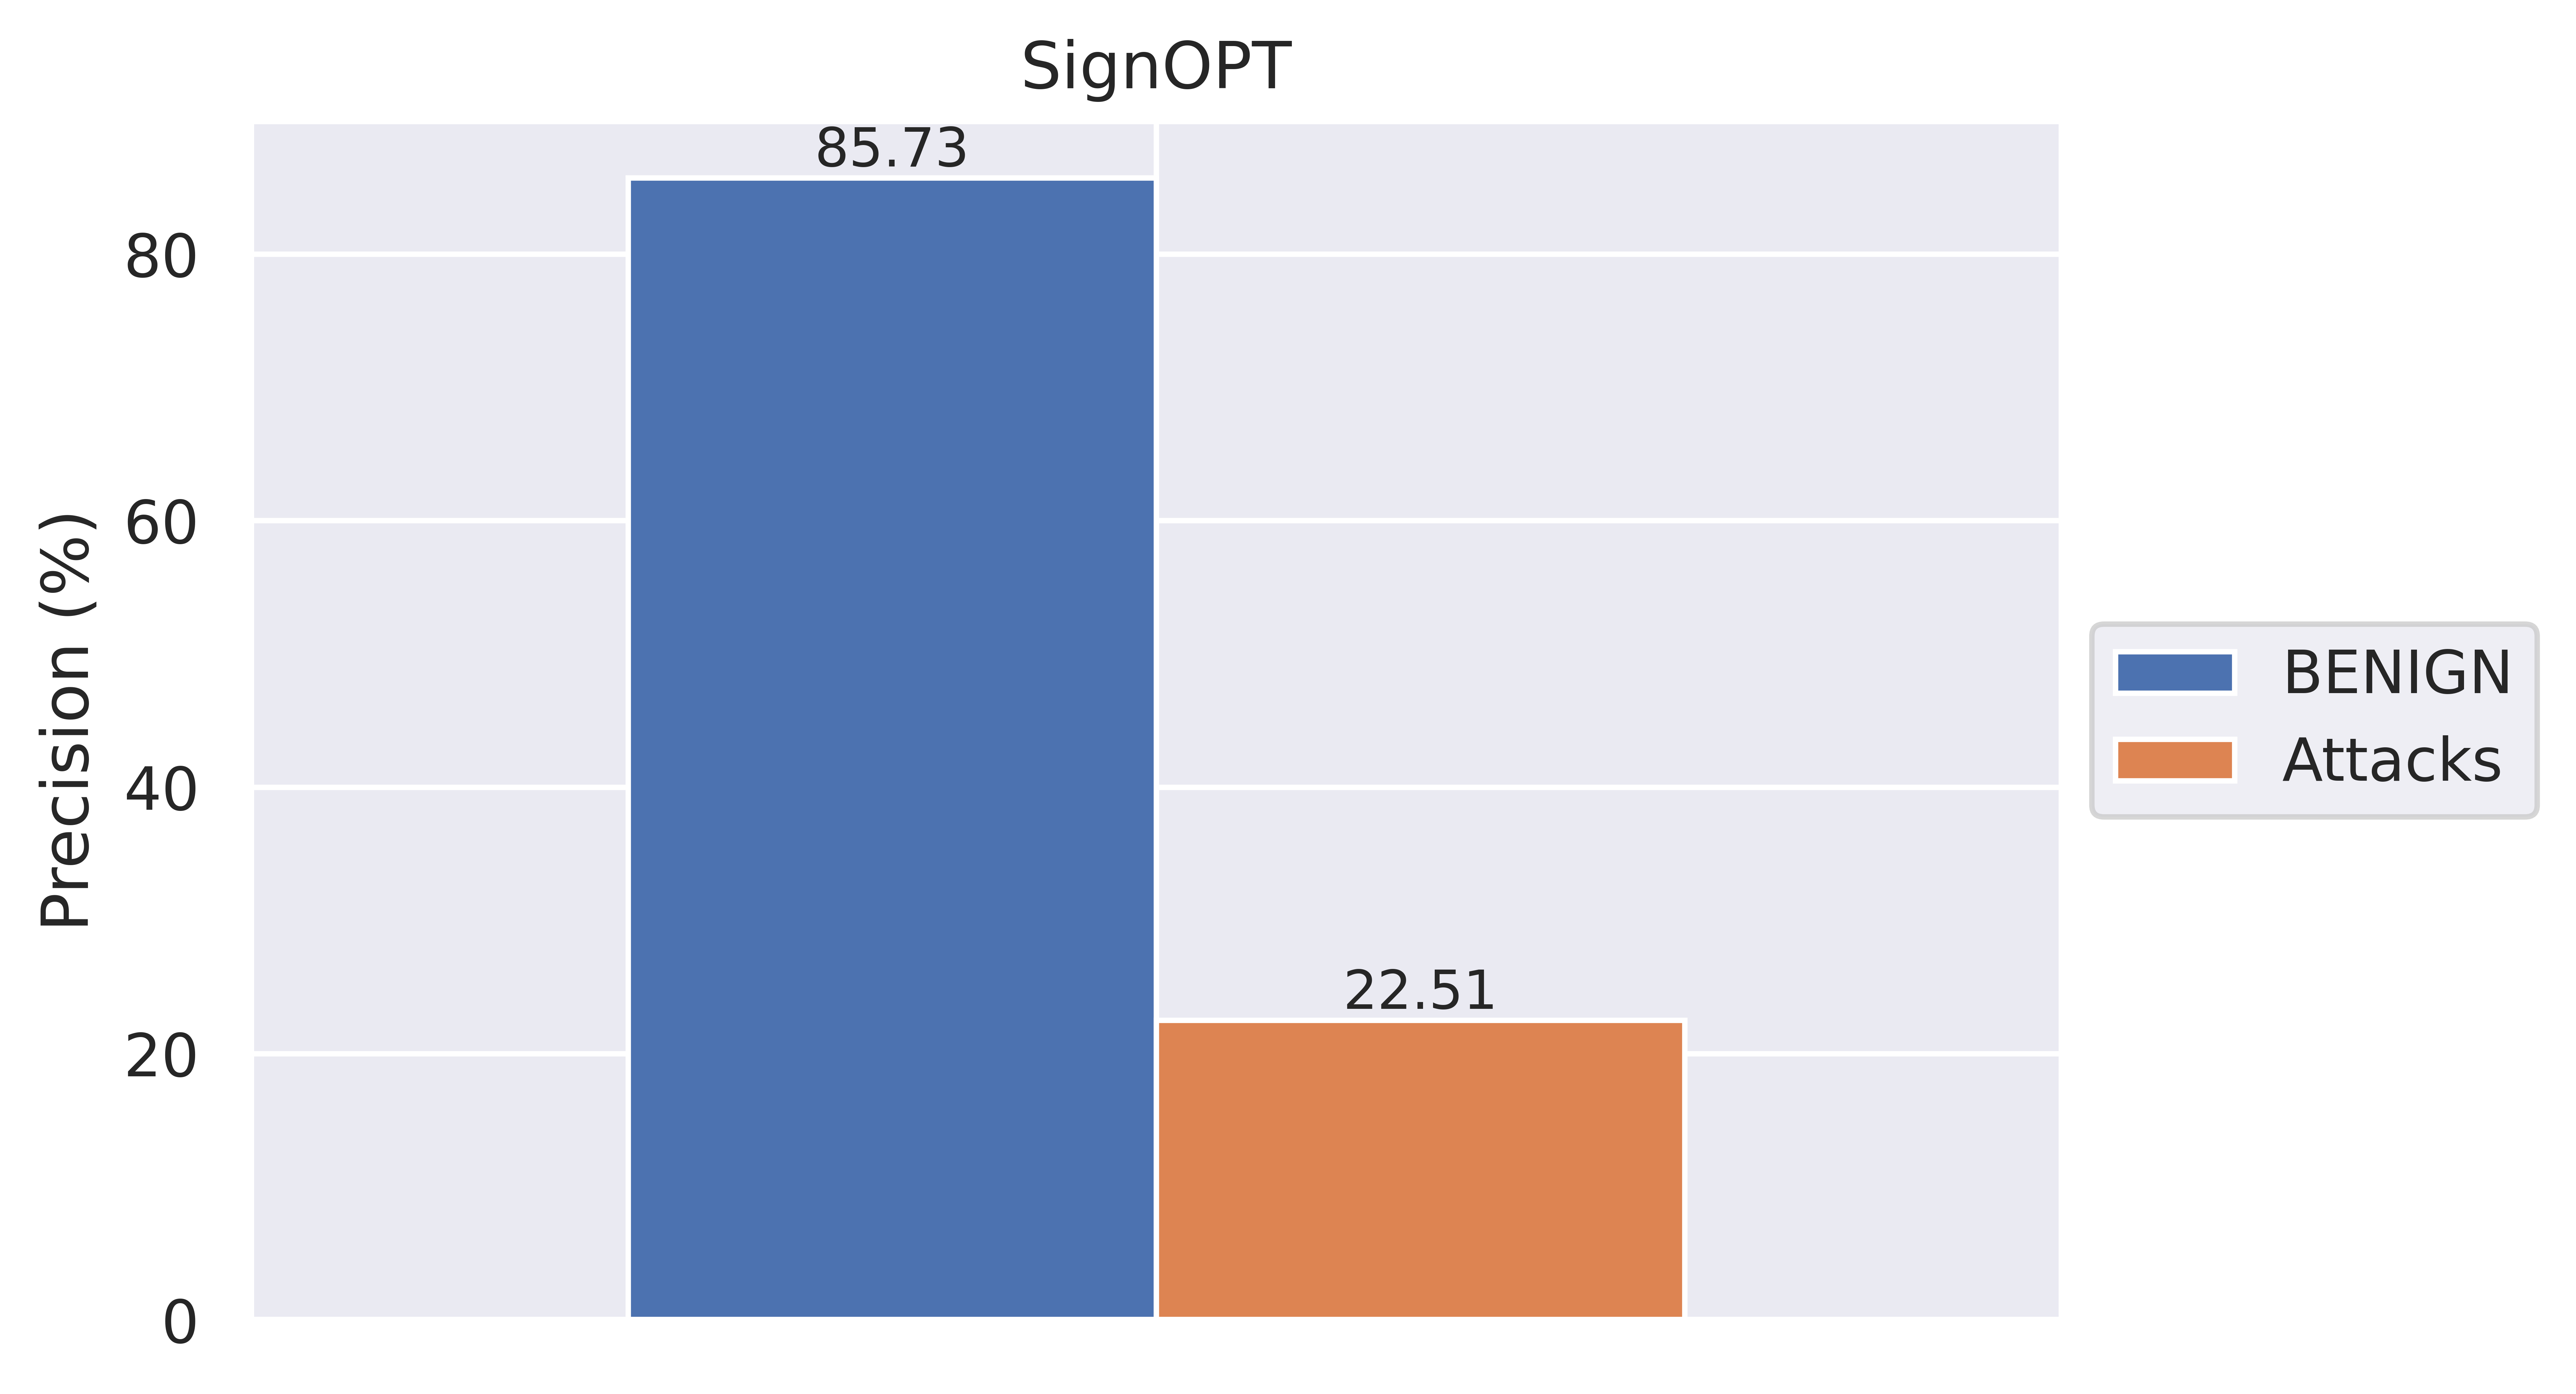
\includegraphics[width=\textwidth]{/home/wojtyla/Documentos/Artigo_2023/IJCNN_Suplementary/Figures//CIC_Clean_SignOPT_bin_paper.png}
			%caption{Figure}
			\label{fig:3}
		\end{subfigure}
		
		
		\vskip\baselineskip
		
		\begin{subfigure}[b]{0.3\textwidth}
			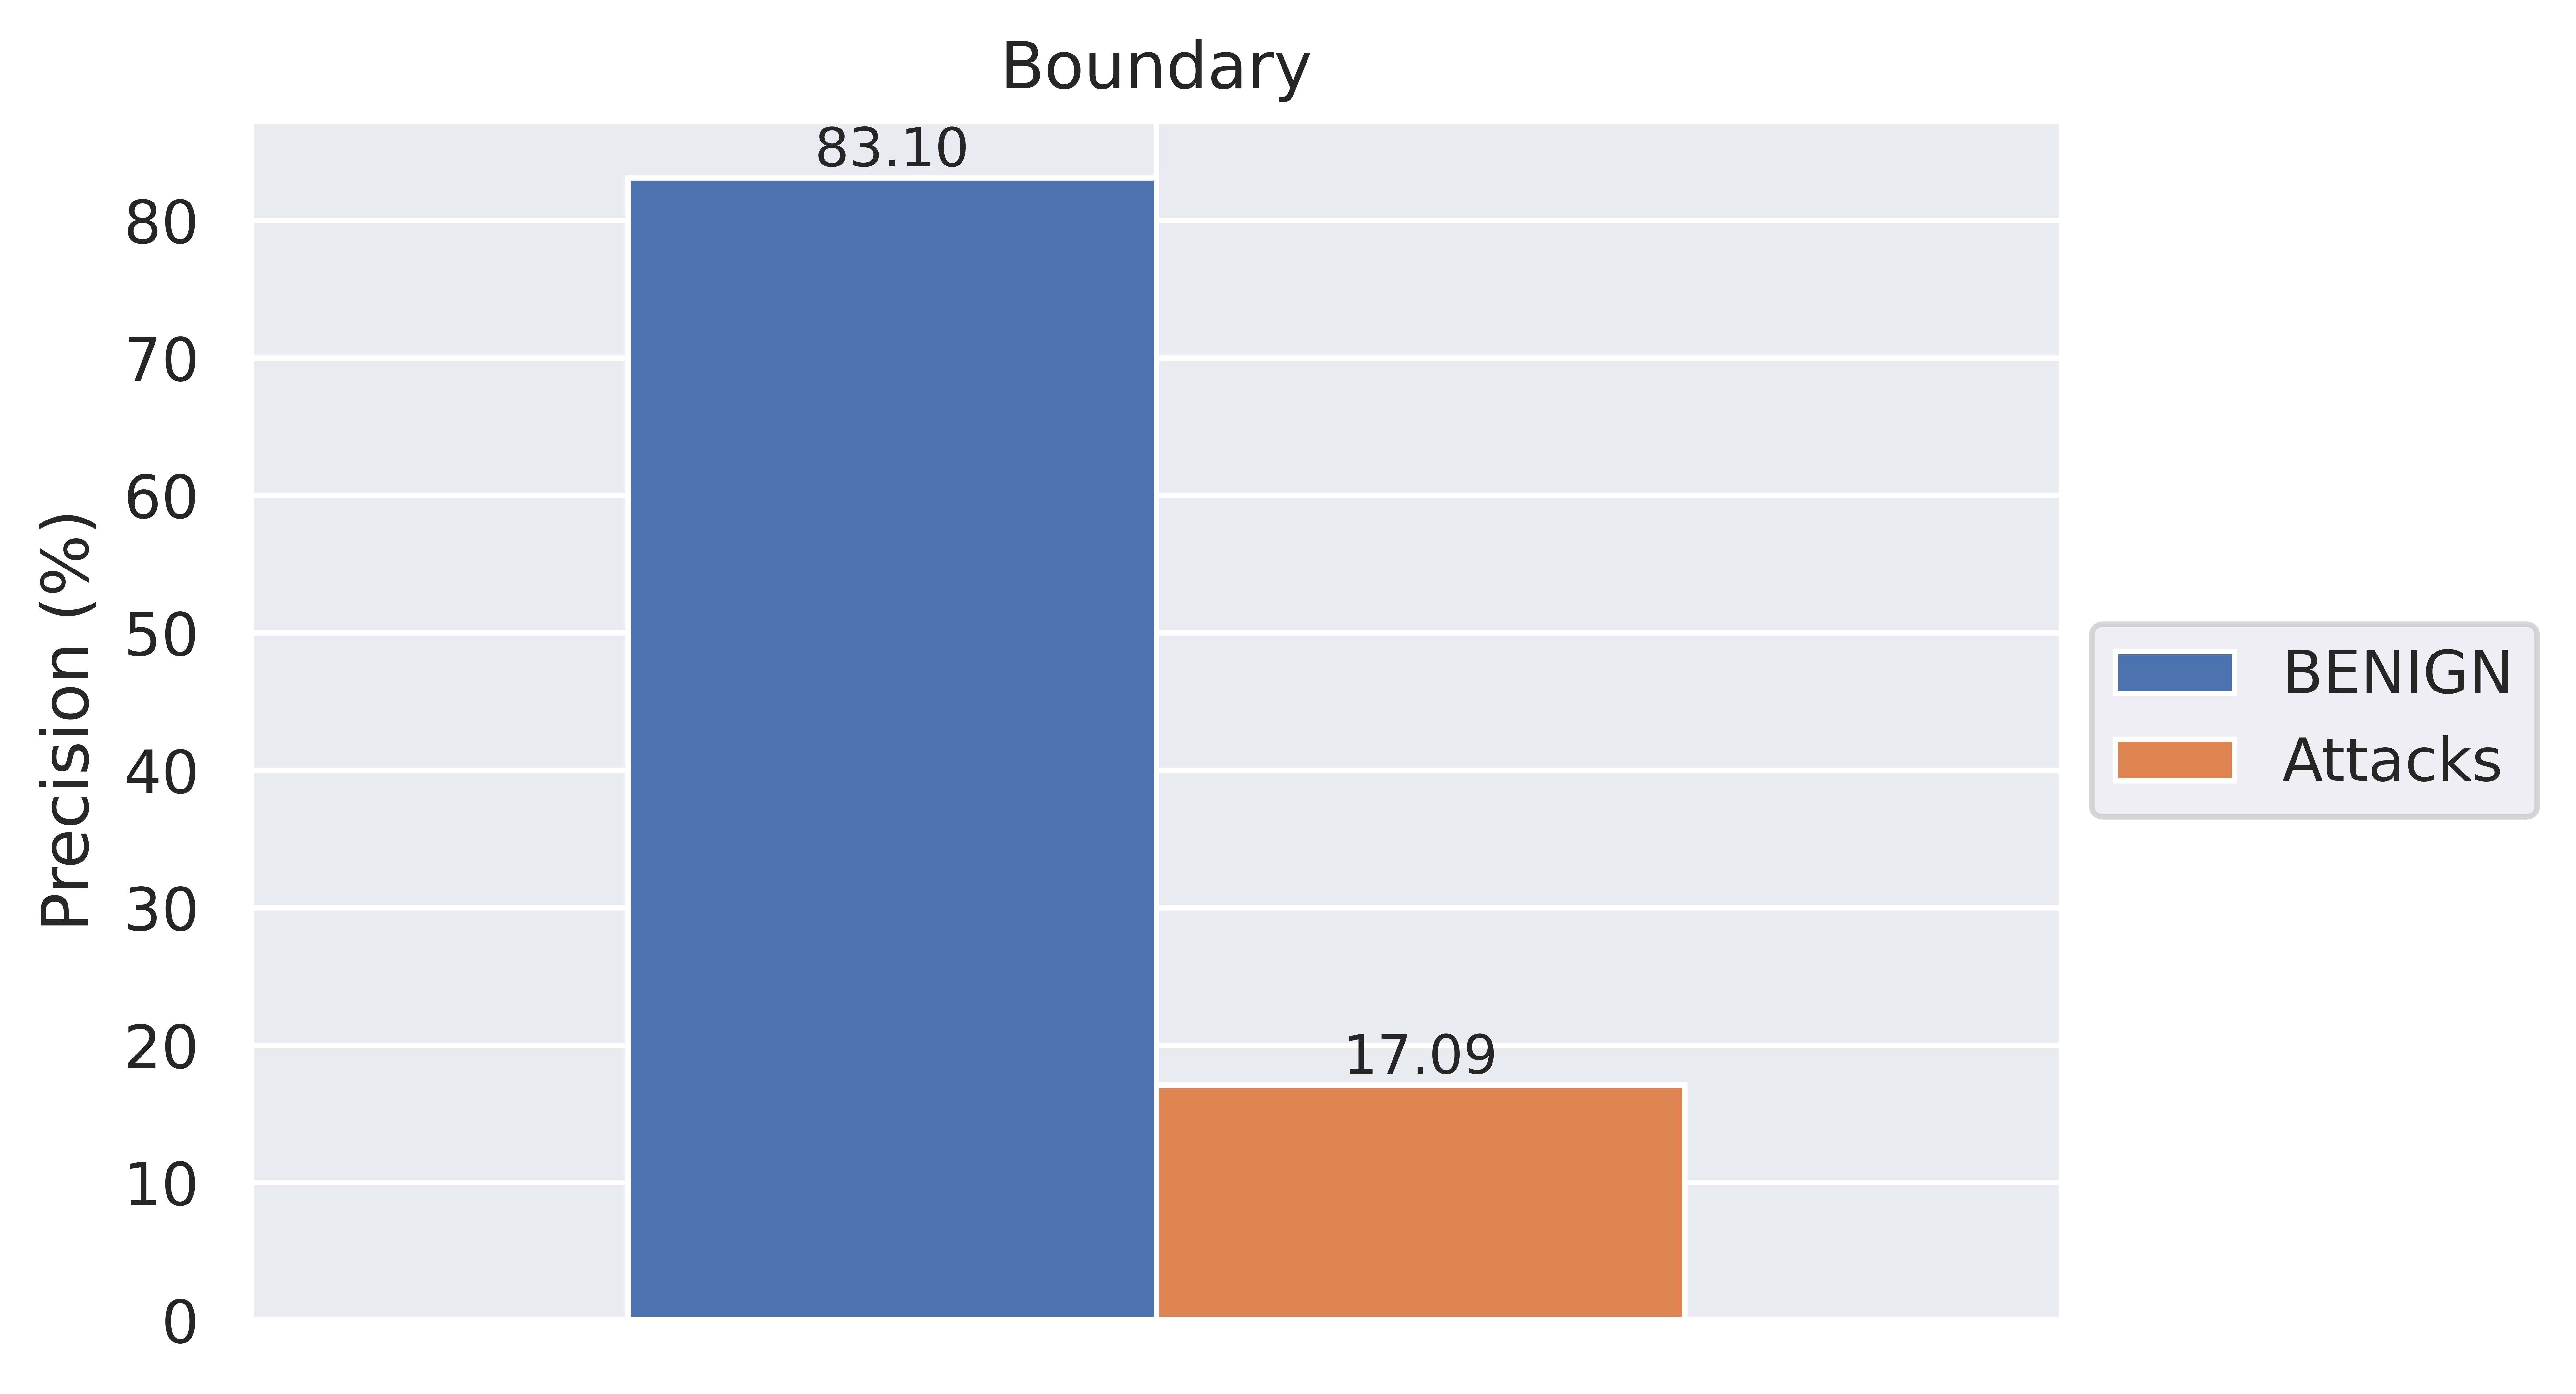
\includegraphics[width=\textwidth]{/home/wojtyla/Documentos/Artigo_2023/IJCNN_Suplementary/Figures//CIC_IDS_Boundary_bin_paper.png}
			%caption{Figure}
			\label{fig:4}
		\end{subfigure}
		\hfill
		\begin{subfigure}[b]{0.3\textwidth}
			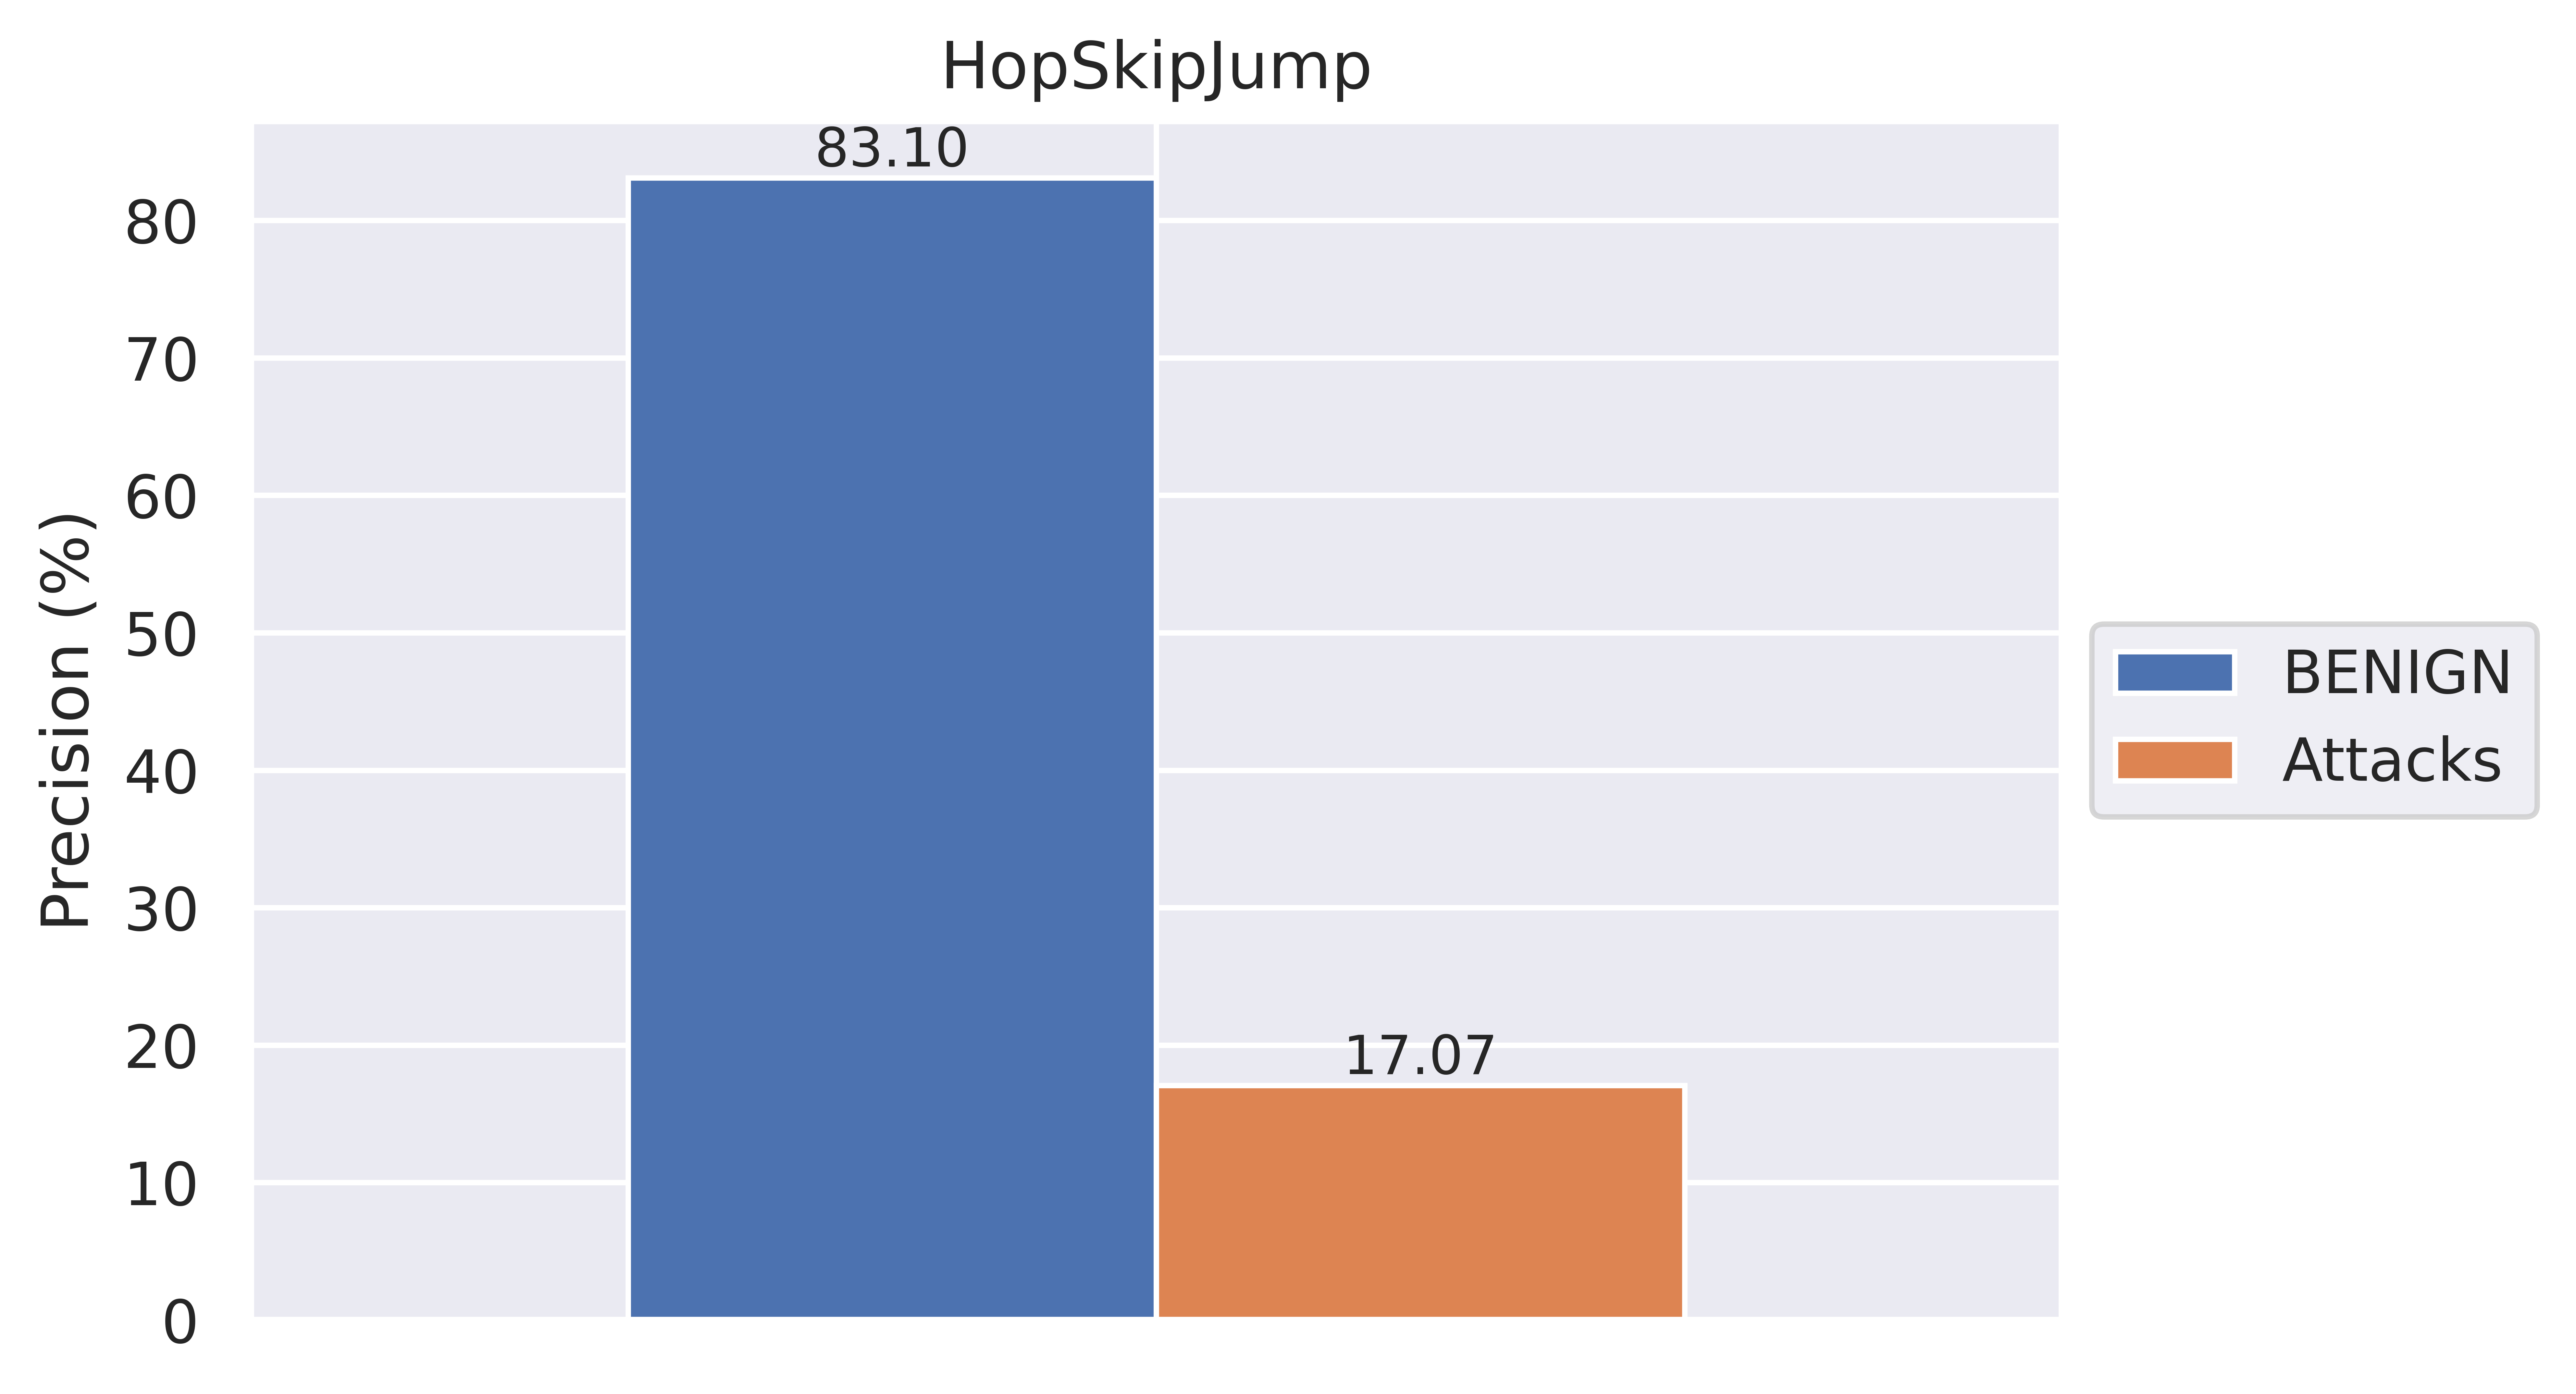
\includegraphics[width=\textwidth]{/home/wojtyla/Documentos/Artigo_2023/IJCNN_Suplementary/Figures//CIC_IDS_HopSkipJump_bin_paper.png}
			%caption{Figure}
			\label{fig:5}
		\end{subfigure}
		\hfill
		\begin{subfigure}[b]{0.3\textwidth}
			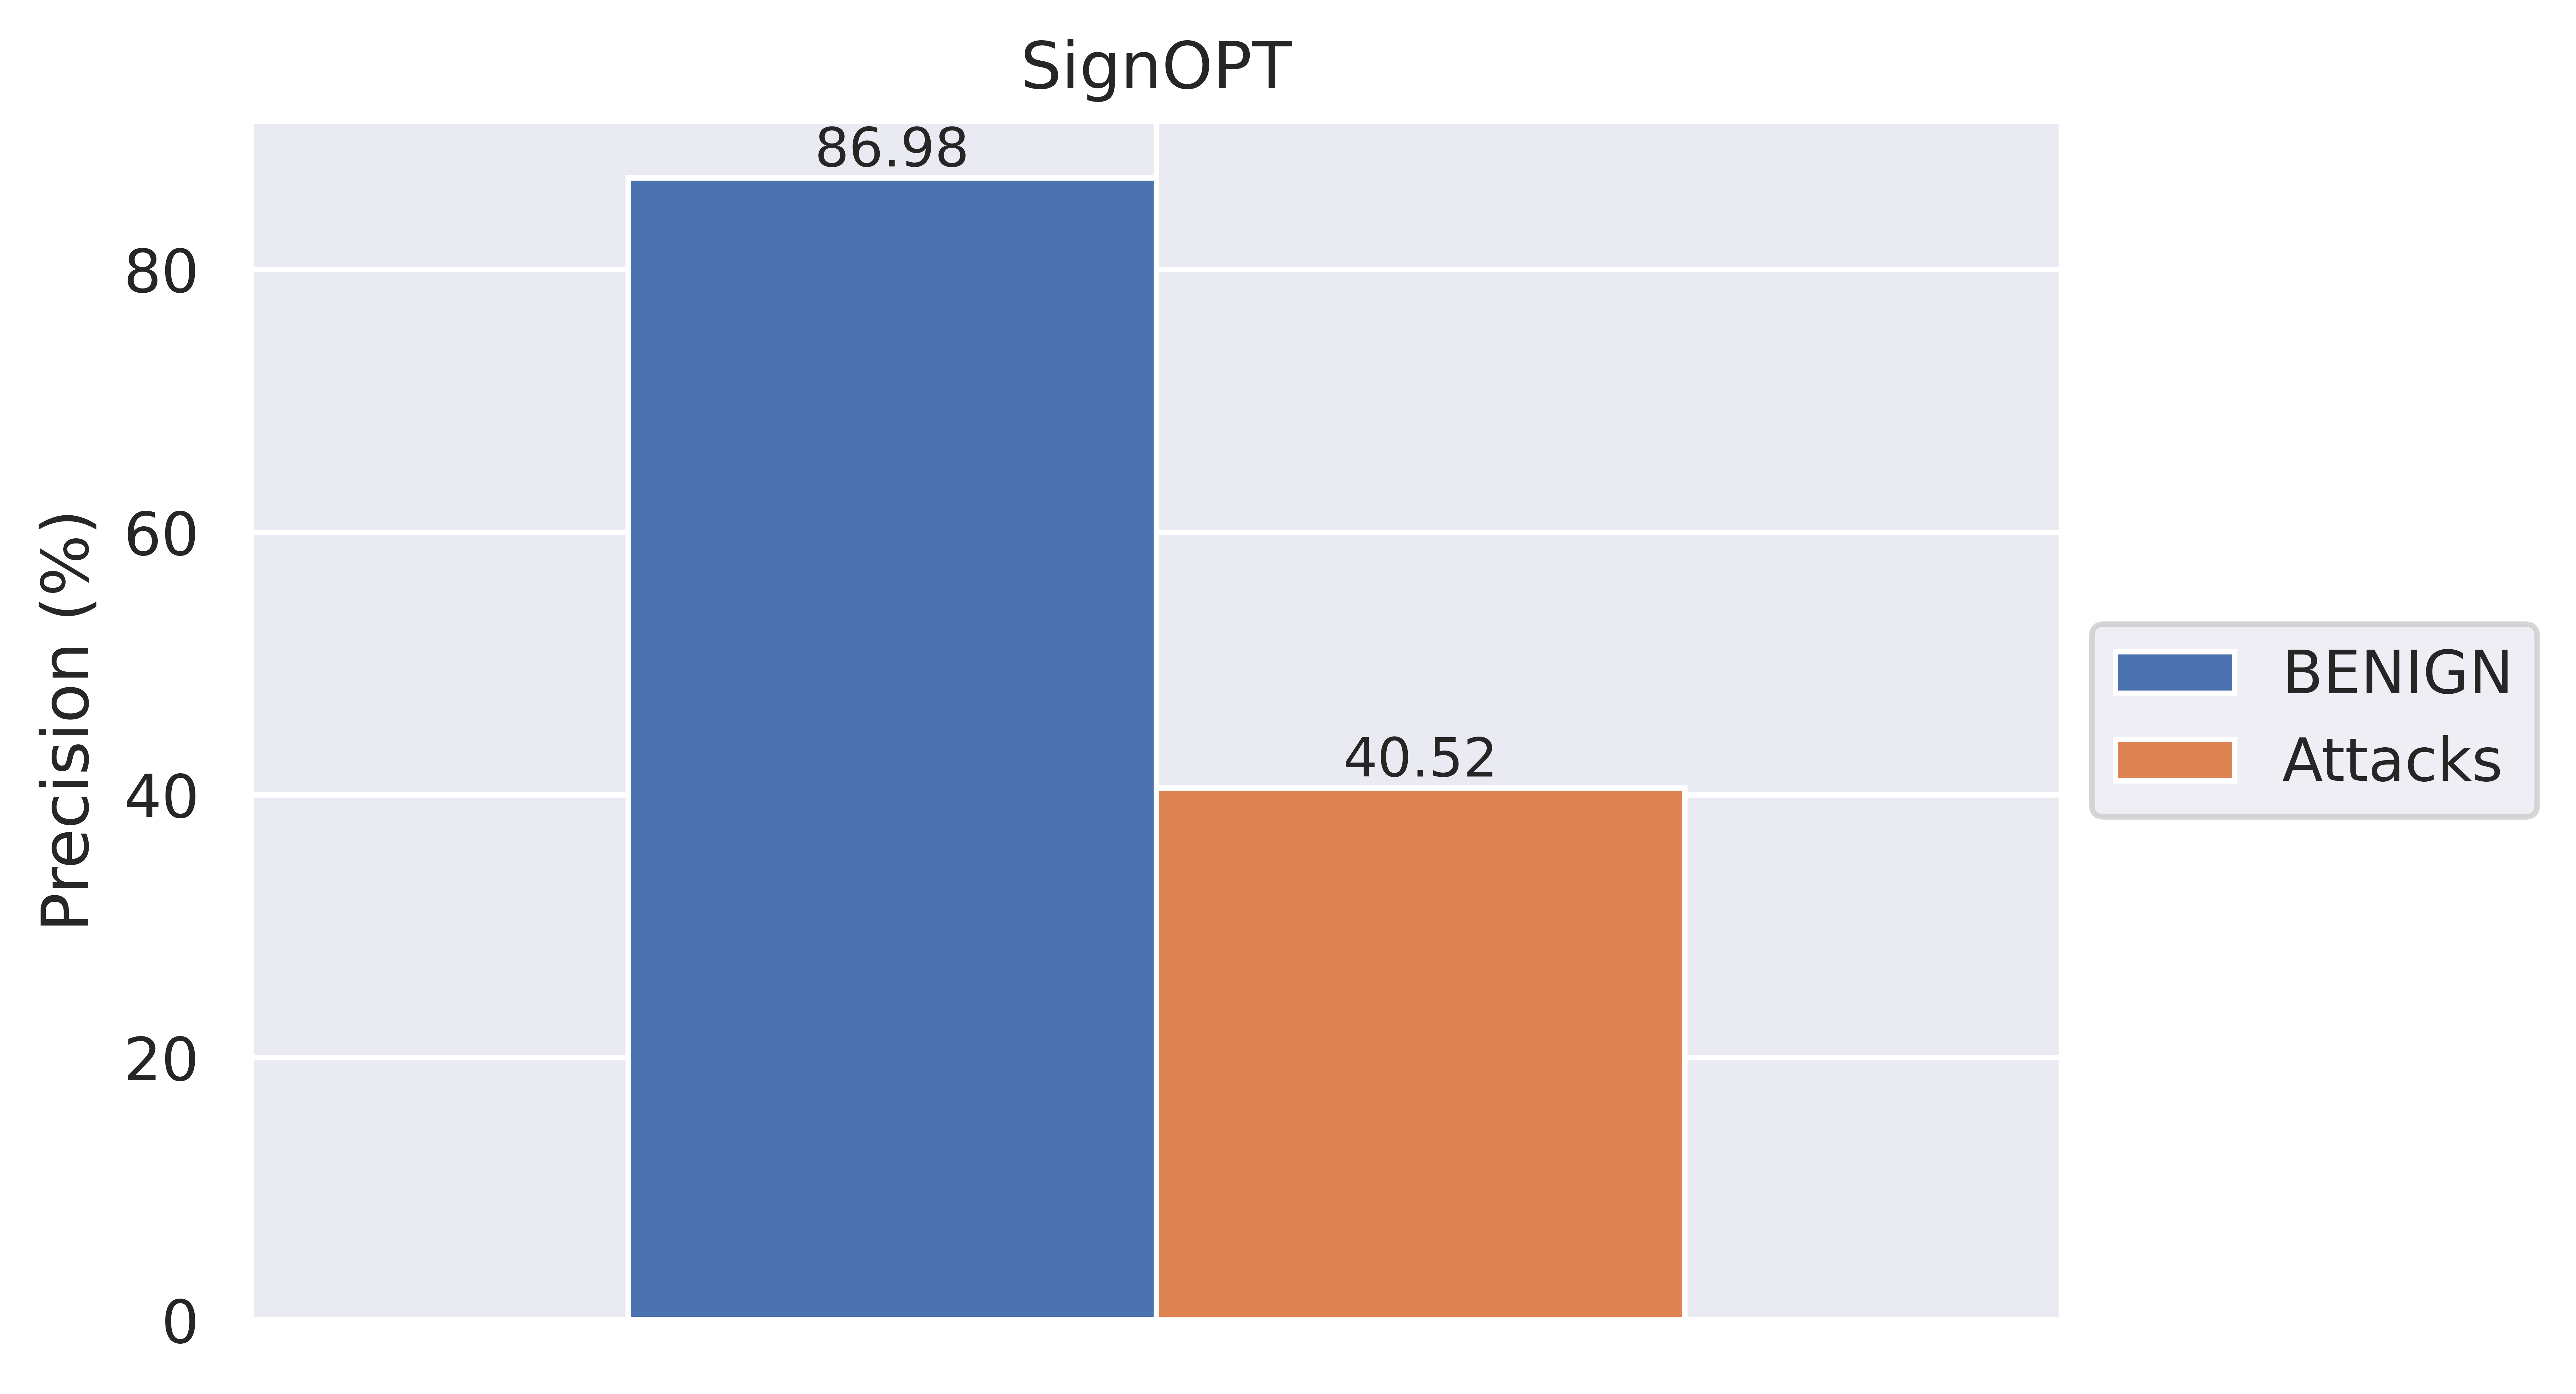
\includegraphics[width=\textwidth]{/home/wojtyla/Documentos/Artigo_2023/IJCNN_Suplementary/Figures//CIC_IDS_SignOPT_bin_paper.png}
			%caption{Figure}
			\label{fig:6}
		\end{subfigure}
		\caption{Plots for black-box attacks on binary models with CIC IDS2017.Top:EnC model; Bottom:EnIDS model.}			
		\label{fig:cic_black_bin}
	\end{figure}
	
	
	
	
	
	\begin{table}[H]
		\caption{Black-Box attacks against EnC and EnIDS for multiclass classification on the CIC IDS2017 dataset.}
		\small
		\setlength{\tabcolsep}{0.1pt}
		\centering
		\label{tab:cic_multi_black}
		\begin{tabular}{|c|c|c|c|c|c|}
			\hline
			\multirow{2}{*}{\textbf{Type}} & \multirow{2}{*}{\textbf{Attacks}} & \multirow{2}{*}{\textbf{Metrics}} & \multicolumn{3}{c|}{\textbf{Label}} \\
			\cline{4-6}
			&  &  & \textbf{\textsl{Benign}} & \textbf{\textsl{DoS}} & \textbf{\textsl{DDoS}}
			\\
			\hline
			\multirow{9}{*}{EnC} & \multirow{3}{*}{Boundary} & Precision & 83.10 & 10.44 & 10.28
			\\
			
			&  & Recall & 57.43 & 4.47 & 0.06
			\\
			
			&  & ROC-AUC & 49.91 & 45.61 & 46.71
			\\
			\cline{2-6}
			& \multirow{3}{*}{HopSkipJump} & Precision & 79.79 & 13.37 & 4.71
			\\
			
			&  & Recall & 57.59 & 4.67 & 0.02
			\\
			
			&  & ROC-AUC & 63.25 & 95.63 & 99.87
			\\
			\cline{2-6}
			& \multirow{3}{*}{SignOPT} & Precision & 81.84 & 18.73 & 21.05
			\\
			
			&  & Recall & 60.70 & 11.31 & 1.16
			\\
			
			&  & ROC-AUC & 70.63 & 93.96 & 99.22
			\\
			\hline
			\multirow{9}{*}{EnIDS} & \multirow{3}{*}{Boundary} & Precision & \cellcolor{yellow!50}83.07 & 10.01 & 5.73
			\\
			
			&  & Recall & \cellcolor{yellow!50}72.21 & 11.07 & 3.86
			\\
			
			&  & ROC-AUC & \cellcolor{yellow!50}75.44 & \cellcolor{yellow!50}77.64 & \cellcolor{yellow!50}76.64
			\\
			\cline{2-6}
			& \multirow{3}{*}{HopSkipJump} & Precision & \cellcolor{yellow!50}83.17 & 10.56 & 8.27
			\\
			
			&  & Recall & \cellcolor{yellow!50}72.13 & 11.66 & 3.82
			\\
			
			&  & ROC-AUC & \cellcolor{yellow!50}82.96 & 94.62 & 98.68
			\\
			\cline{2-6}
			& \multirow{3}{*}{SignOPT} & Precision & \cellcolor{yellow!50}86.65 & 23.13 & 34.06
			\\
			
			&  & Recall & \cellcolor{yellow!50}74.11 & 19.78 & 17.69
			\\
			
			&  & ROC-AUC & \cellcolor{yellow!50}88.30 & \cellcolor{yellow!50}96.33 & 98.83
			\\
			\hline
		\end{tabular}
	\end{table}		
	
	\begin{figure}[H]
		\centering
		\begin{subfigure}[b]{0.28\textwidth}
			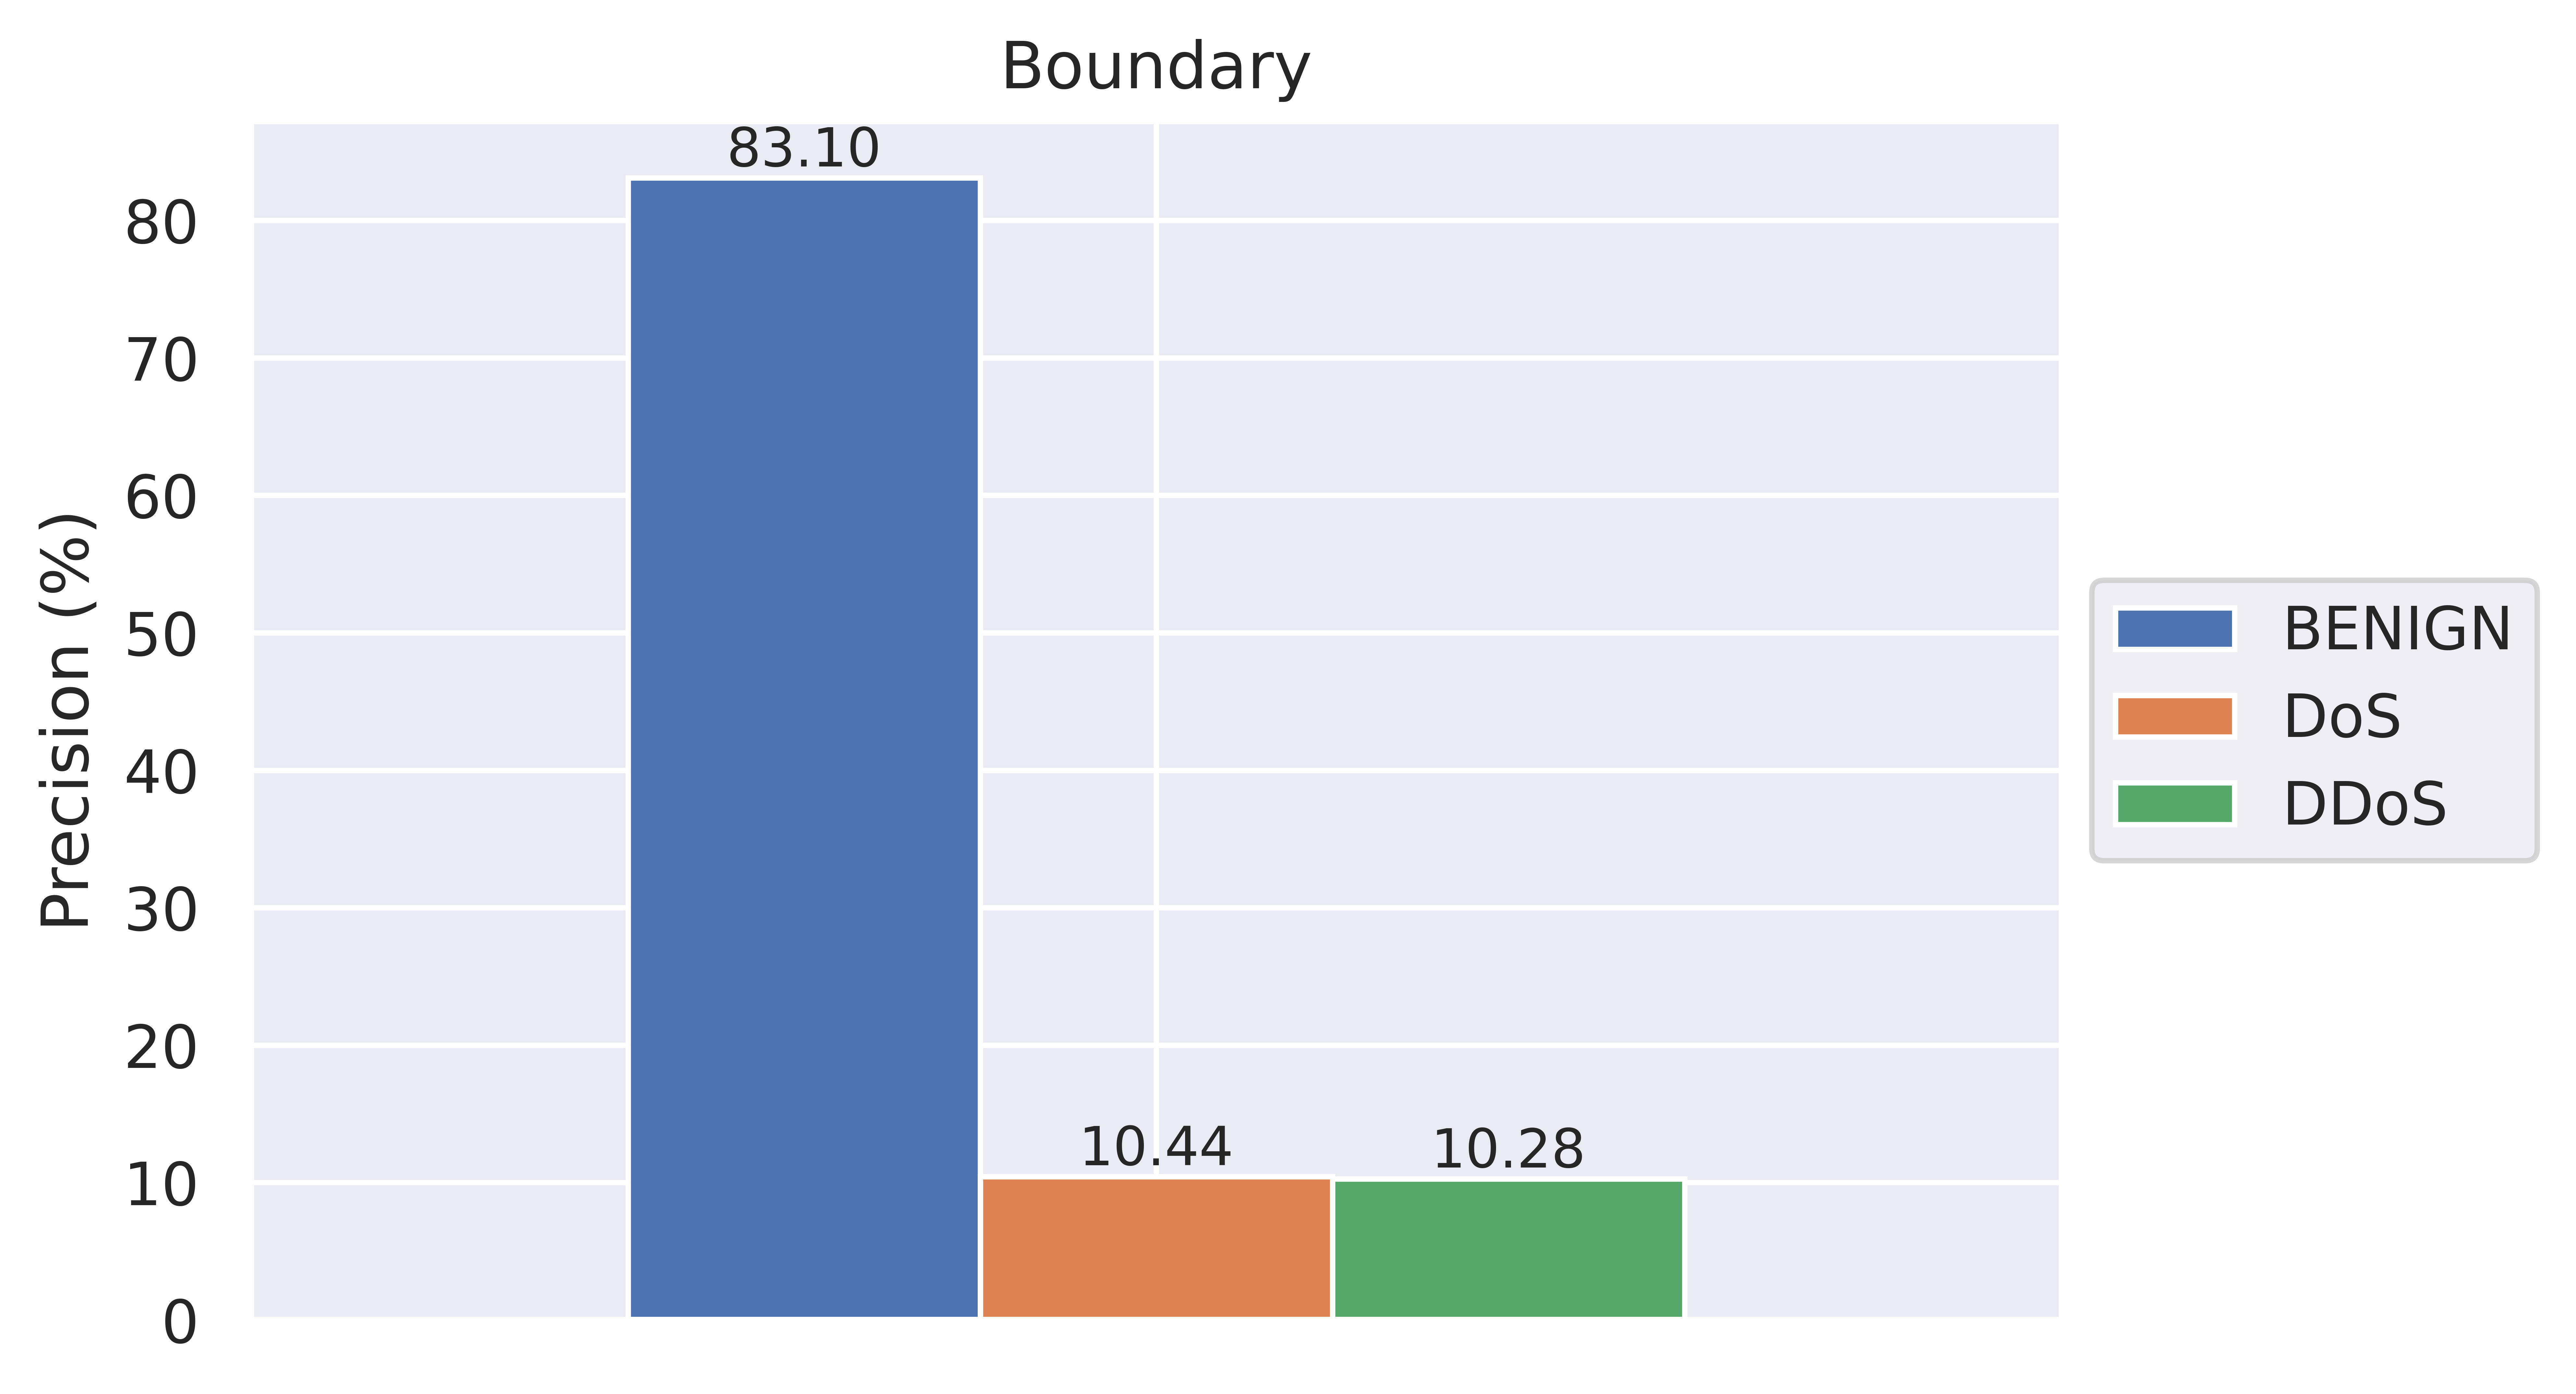
\includegraphics[width=\textwidth]{/home/wojtyla/Documentos/Artigo_2023/IJCNN_Suplementary/Figures//CIC_Clean_Boundary_multi_paper.png}
			%caption{Figure}
			\label{fig:1}
		\end{subfigure}
		\hfill
		\begin{subfigure}[b]{0.28\textwidth}
			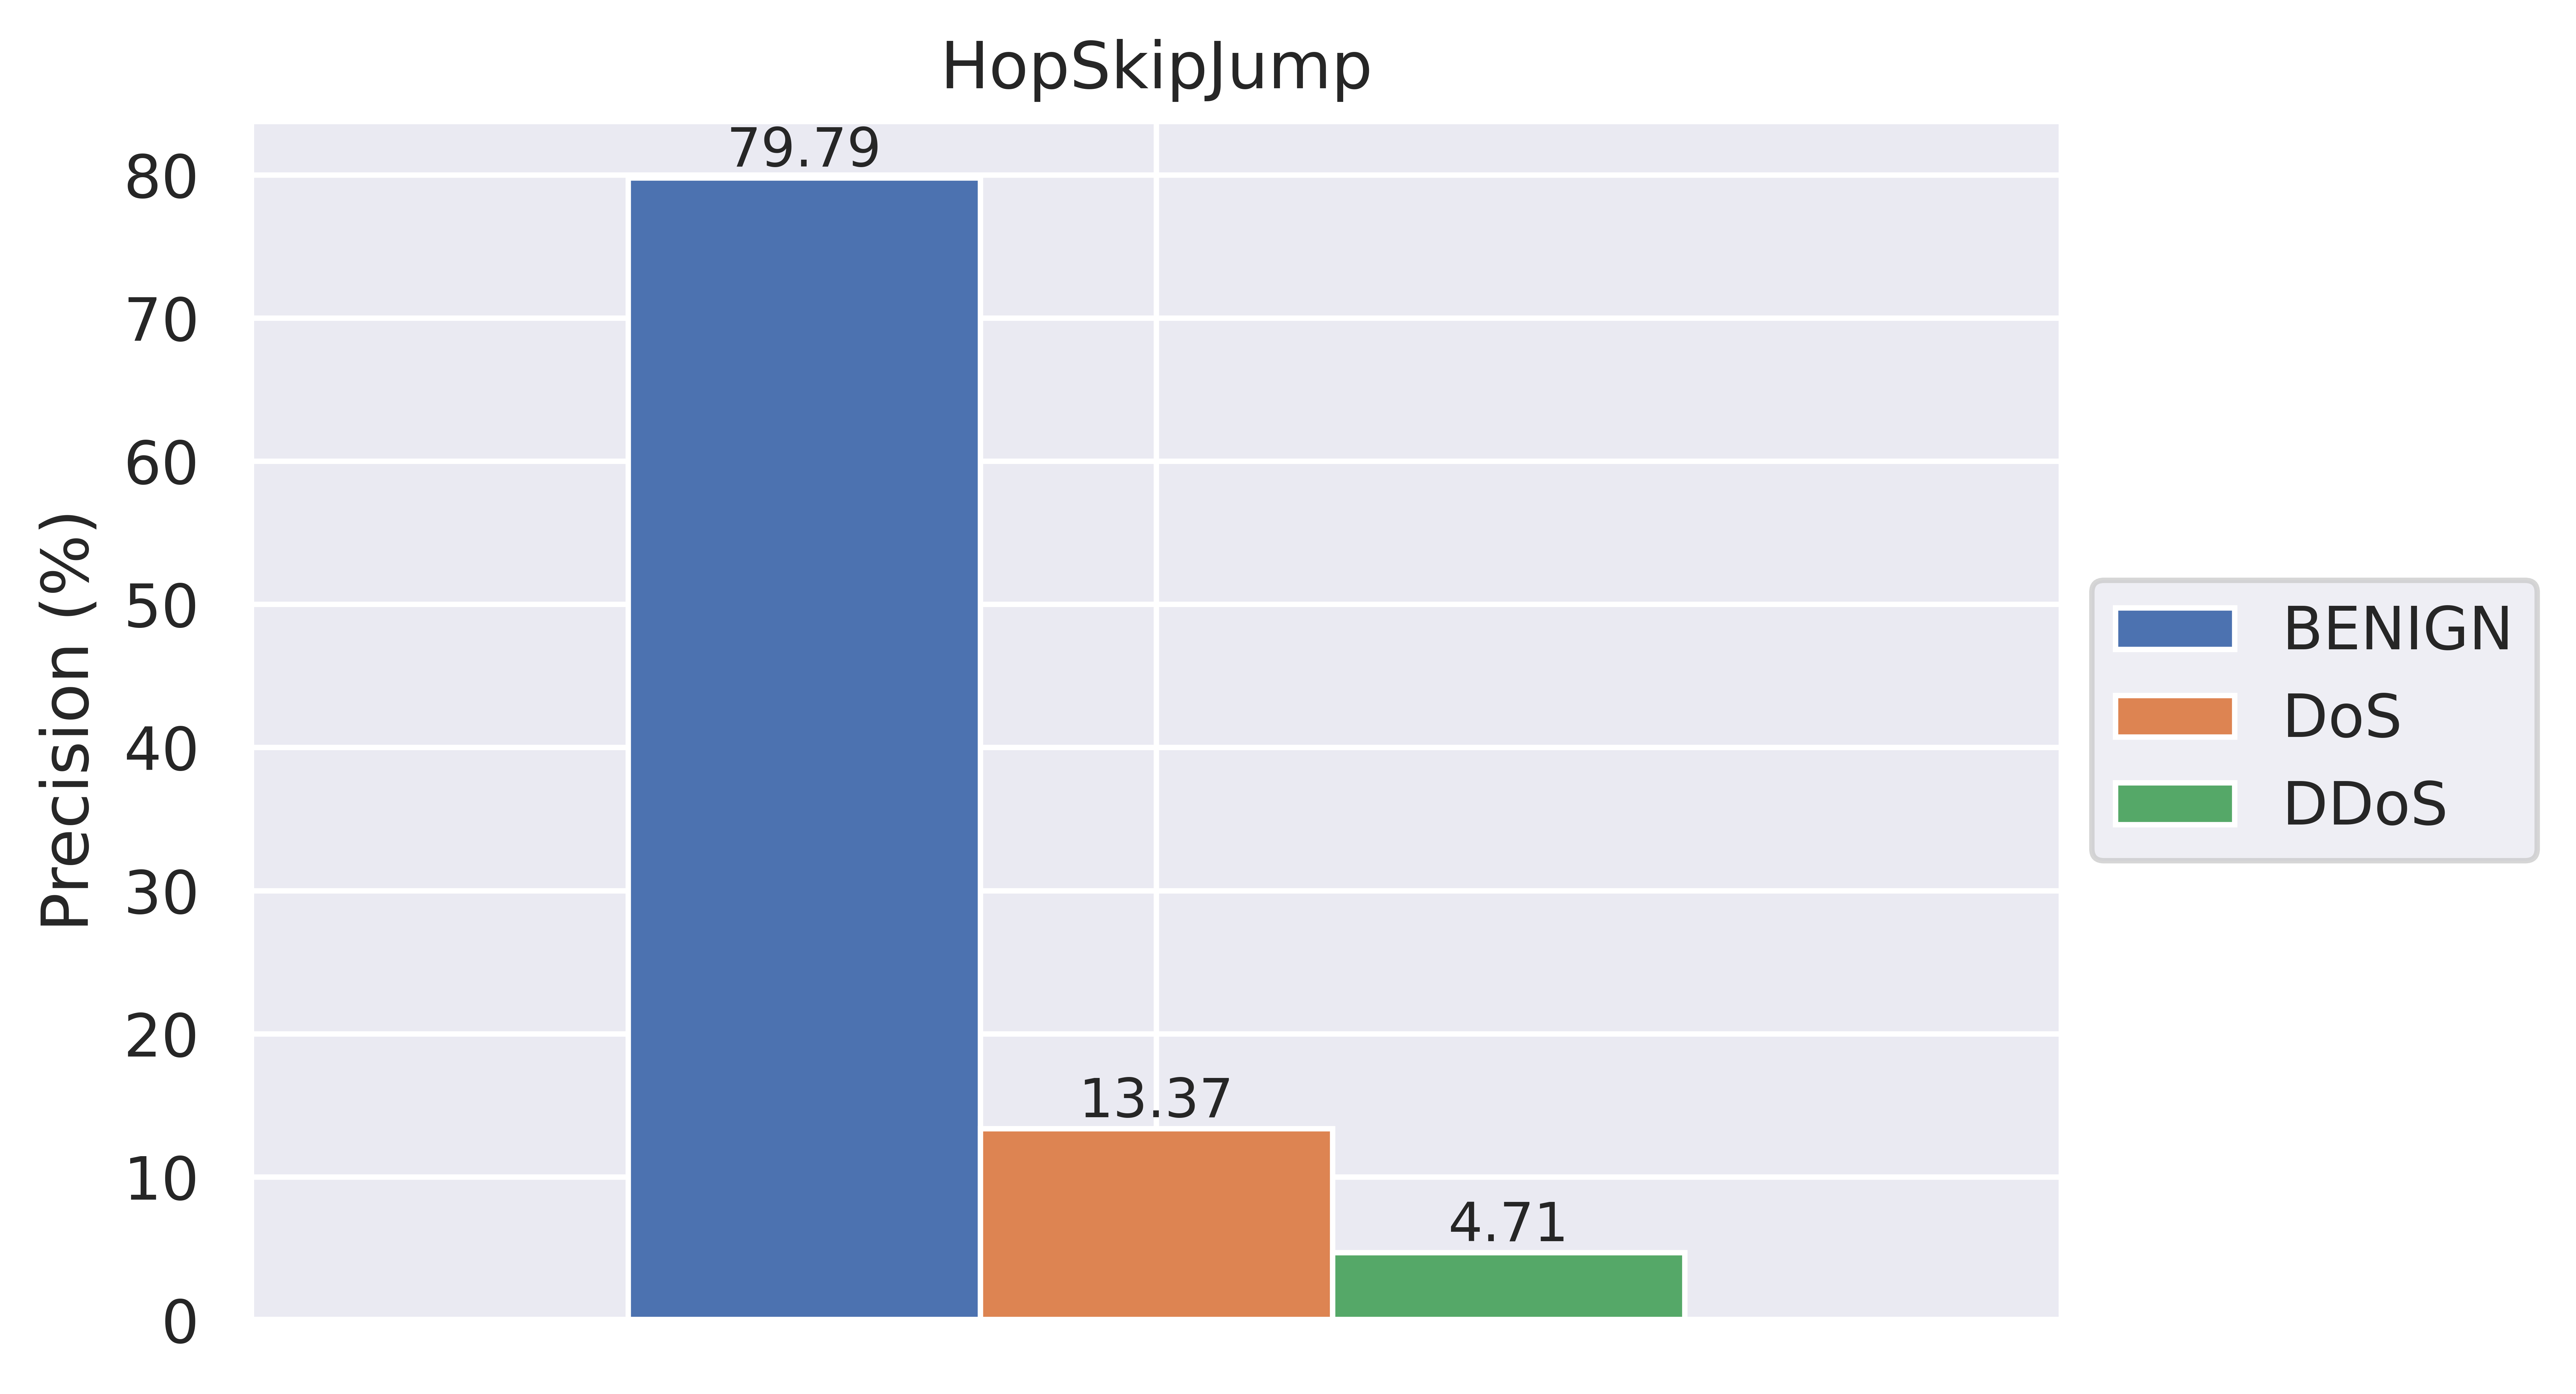
\includegraphics[width=\textwidth]{/home/wojtyla/Documentos/Artigo_2023/IJCNN_Suplementary/Figures//CIC_Clean_HopSkipJump_multi_paper.png}
			%caption{Figure}
			\label{fig:2}
		\end{subfigure}		
		\hfill
		\begin{subfigure}[b]{0.28\textwidth}
			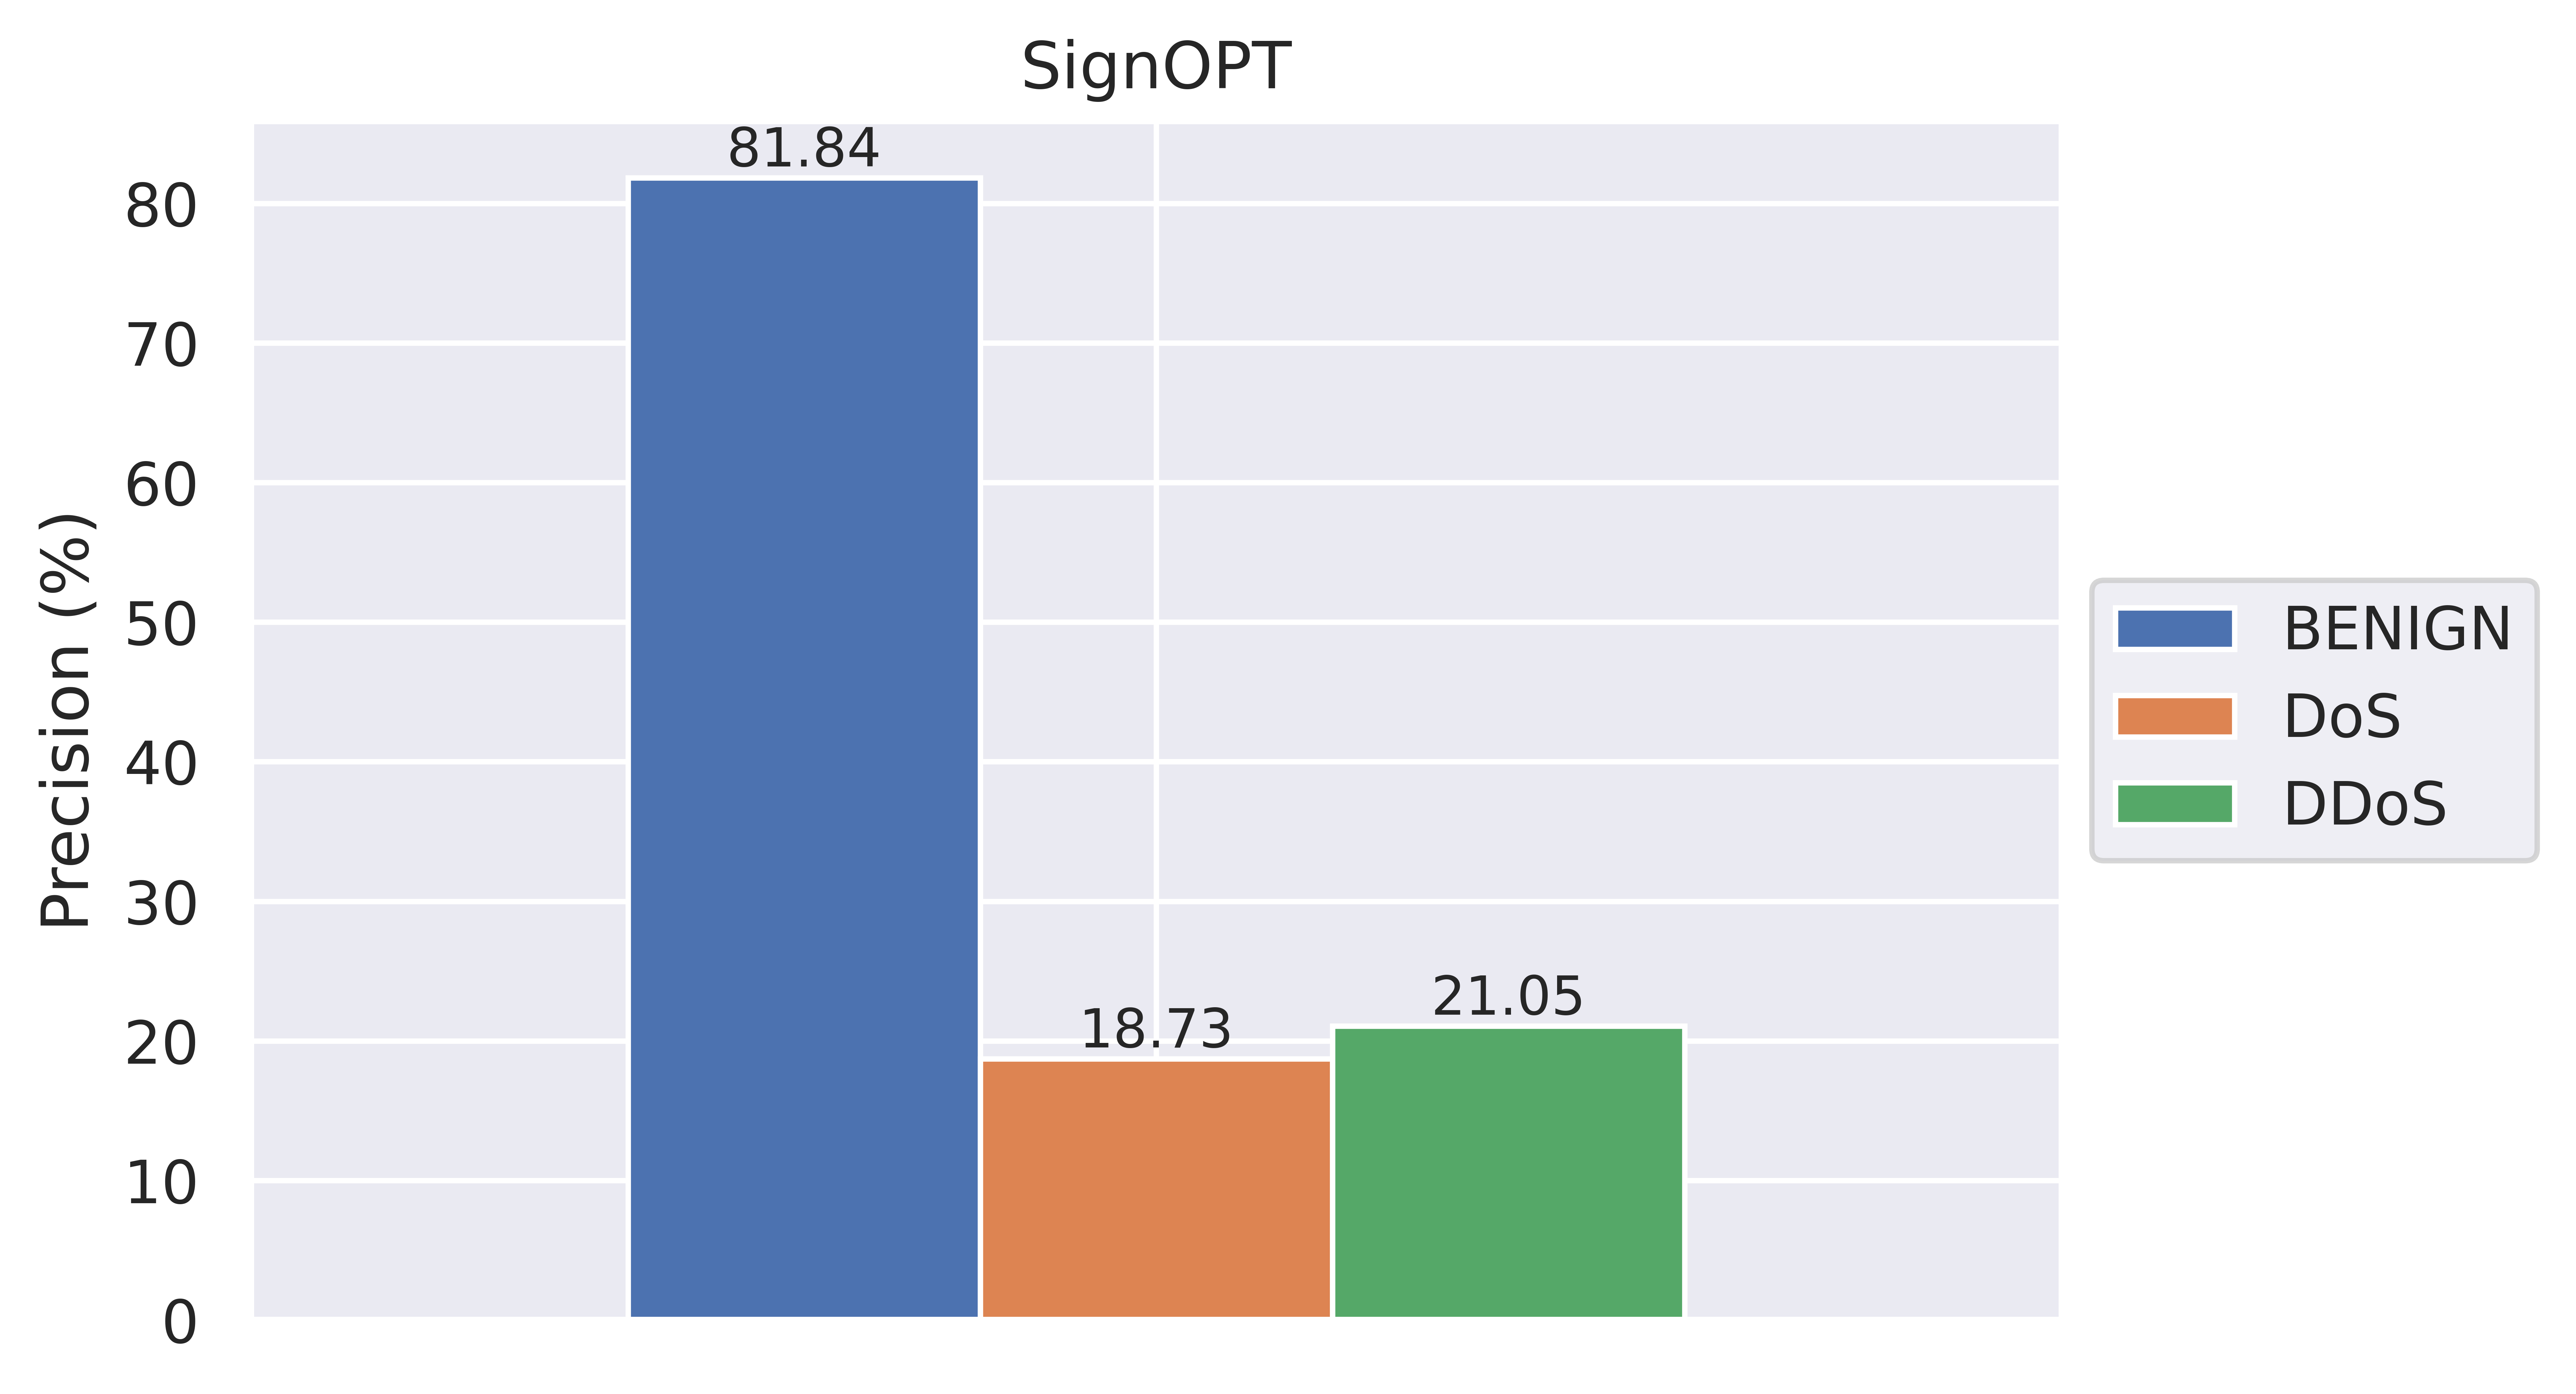
\includegraphics[width=\textwidth]{/home/wojtyla/Documentos/Artigo_2023/IJCNN_Suplementary/Figures//CIC_Clean_SignOPT_multi_paper.png}
			%caption{Figure}
			\label{fig:3}
		\end{subfigure}
		
		\vskip\baselineskip
		
		\begin{subfigure}[b]{0.28\textwidth}
			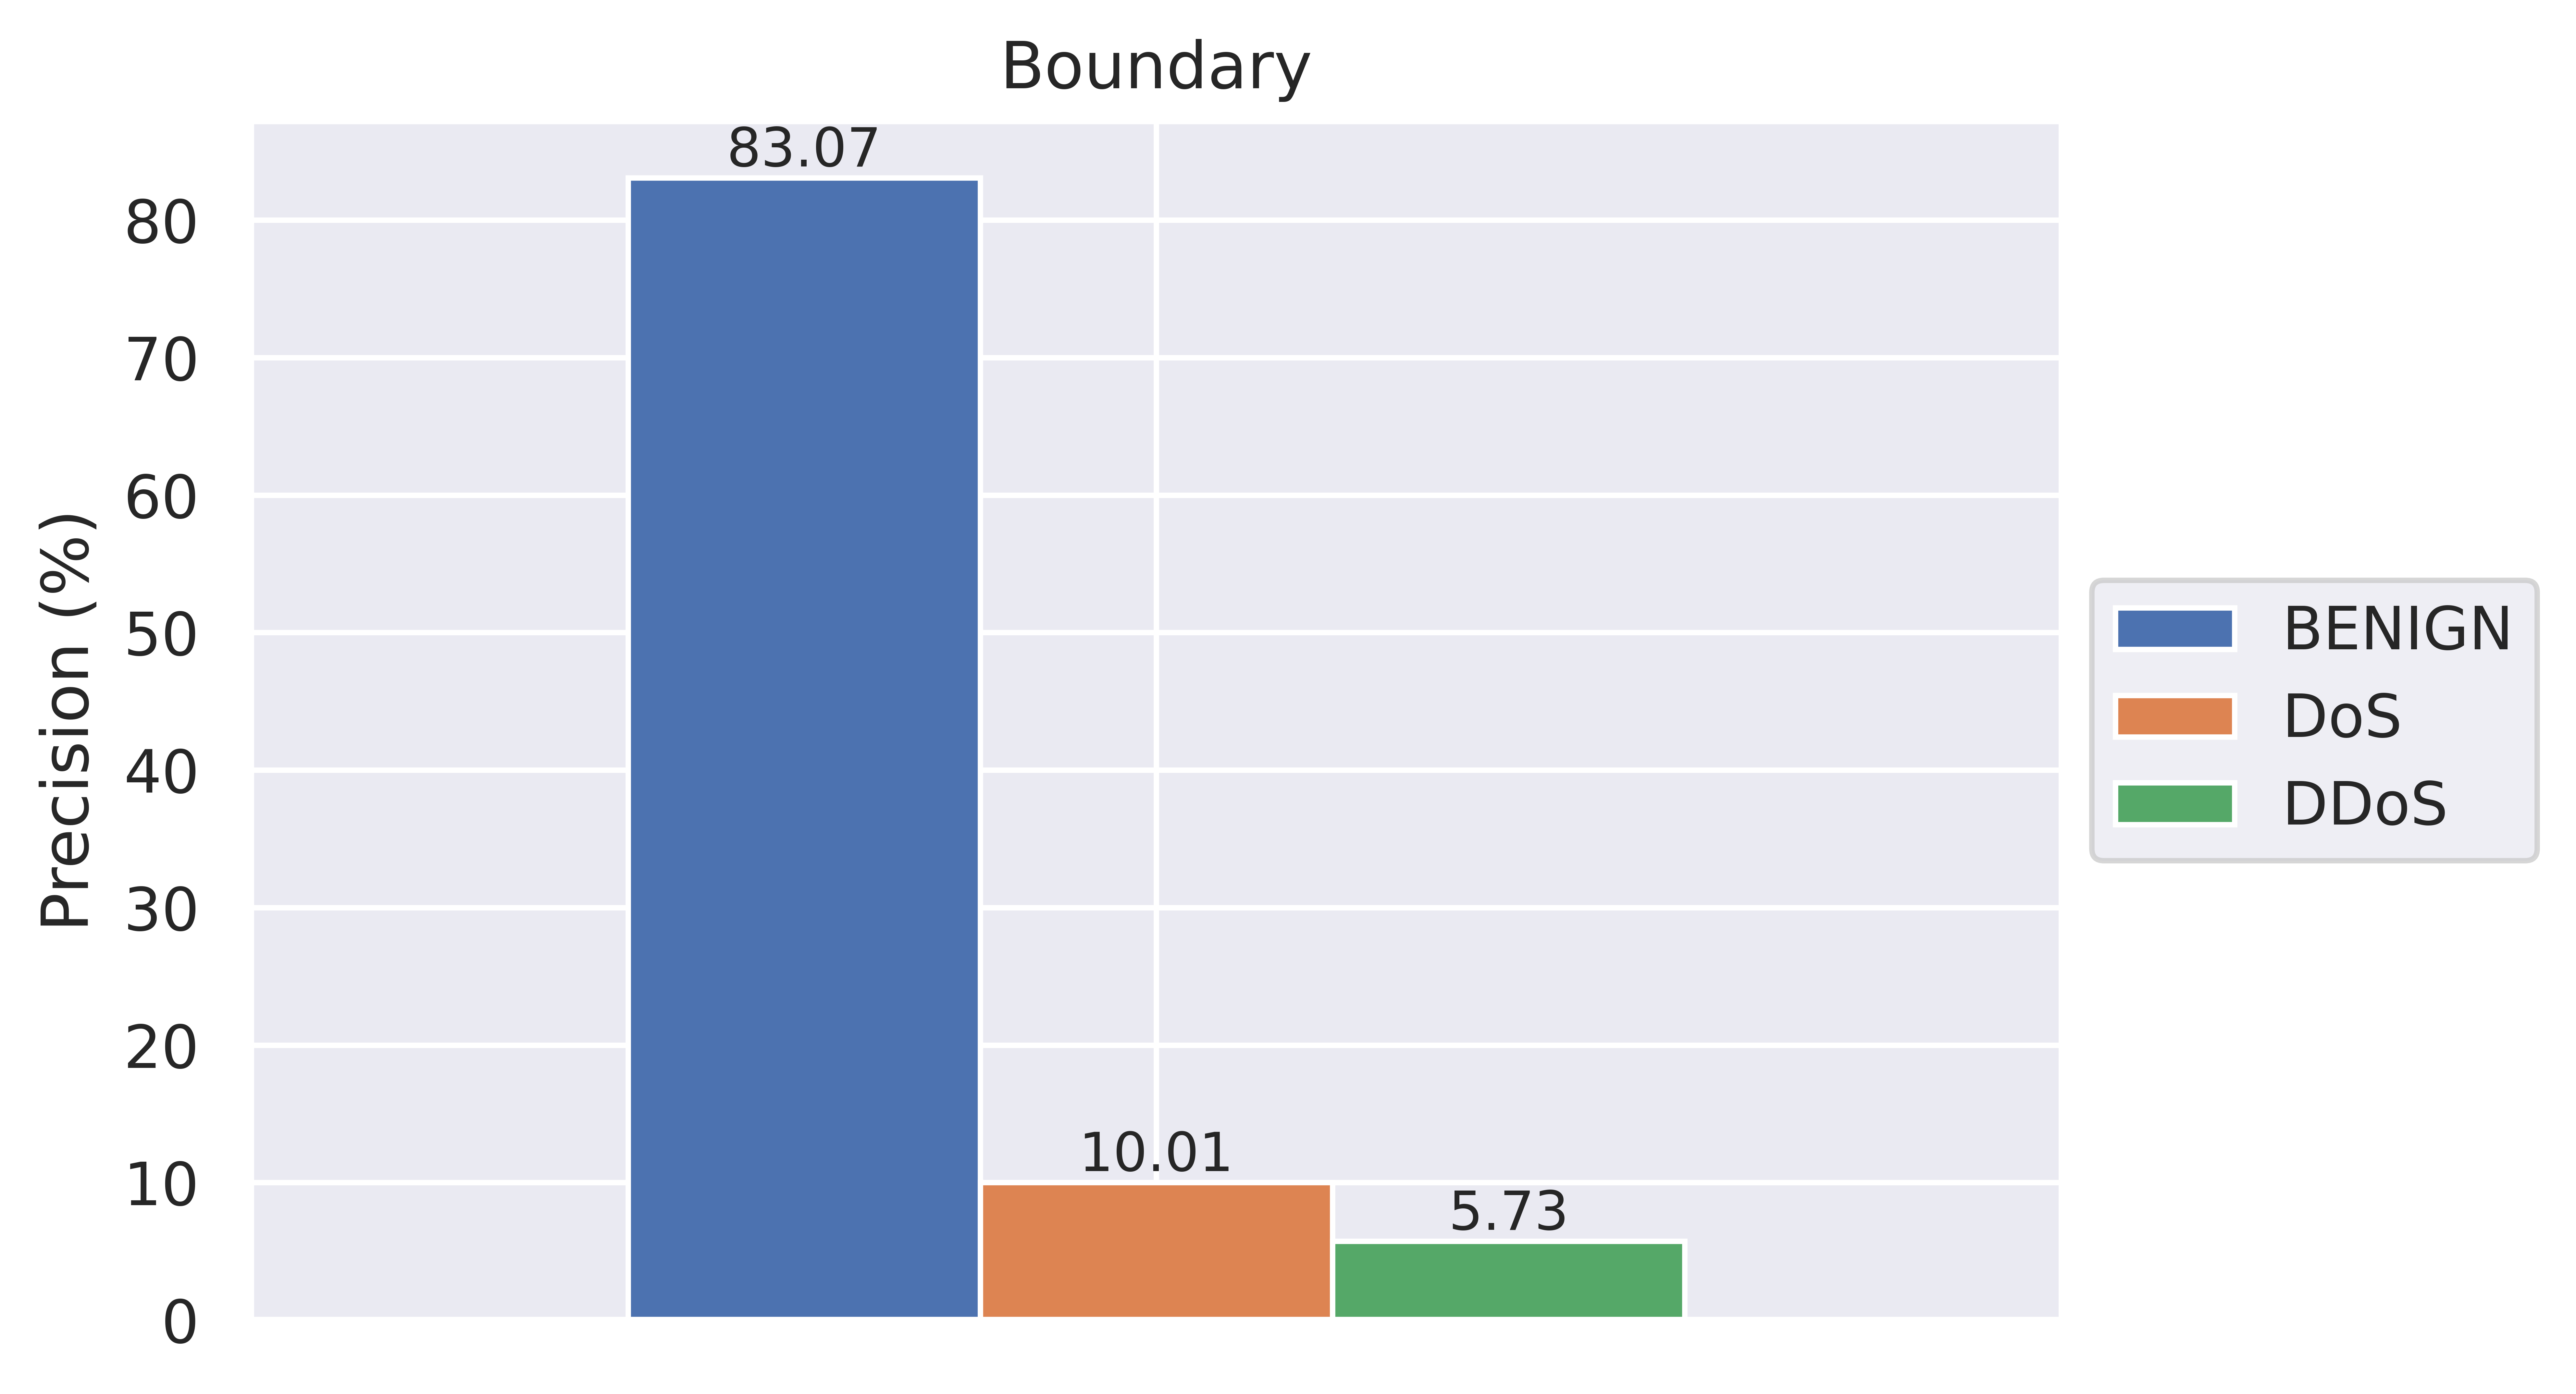
\includegraphics[width=\textwidth]{/home/wojtyla/Documentos/Artigo_2023/IJCNN_Suplementary/Figures//CIC_IDS_Boundary_multi_paper.png}
			%caption{Figure}
			\label{fig:4}
		\end{subfigure}
		\hfill
		\begin{subfigure}[b]{0.28\textwidth}
			\includegraphics[width=\textwidth]{/home/wojtyla/Documentos/Artigo_2023/IJCNN_Suplementary/Figures//CIC_IDS_HopSkipJump_multi_paper.png}
			%caption{Figure}
			\label{fig:5}
		\end{subfigure}		
		\hfill
		\begin{subfigure}[b]{0.28\textwidth}
			\includegraphics[width=\textwidth]{/home/wojtyla/Documentos/Artigo_2023/IJCNN_Suplementary/Figures//CIC_IDS_SignOPT_multi_paper.png}
			%caption{Figure}
			\label{fig:6}
		\end{subfigure}
		\caption{Plots for black-box attacks on multiclass models with CIC IDS2017.Top:EnC model; Bottom:EnIDS model}
		
		\label{fig:cic_black_multi}
	\end{figure}
	
	
	
	
	\subsection{UNSW-NB15}
	
	\begin{table}[H]
		\caption{Black-Box Attacks against EnC and EnIDS for binary classification on the UNSW-NB15 Dataset.}
		\small
		\setlength{\tabcolsep}{1pt}
		\centering
		\label{tab:unsw_bin_black}
		
		\begin{tabular}{|c|c|c|c|c|}
			\hline
			\multirow{2}{*}{\textbf{Type}} & \multirow{2}{*}{\textbf{Attacks}} & \multirow{2}{*}{\textbf{Metrics}} &  \multicolumn{2}{c|}{\textbf{Label}} \\
			\cline{4-5}
			&  &  & \textbf{Normal} & \textbf{Attacks} \\
			\hline
			\multirow{9}{*}{EnC} & 	\multirow{3}{*}{Boundary} & Precision & 97.95 & 2.01
			\\
			
			&  & Recall & 89.46 & 10.38
			\\
			
			&  & ROC-AUC & 51.94 & 64.94
			\\
			\cline{2-5}
			& \multirow{3}{*}{HopSkipJump} & Precision & 97.95 & 1.95
			\\
			
			&  & Recall & 89.45 & 10.06
			\\
			
			&  & ROC-AUC & 90.36 & 90.37
			\\
			\cline{2-5}
			& \multirow{3}{*}{SignOPT} & Precision & 98.50 & 6.71
			\\
			
			&  & Recall & 90.01 & 34.46
			\\
			
			&  & ROC-AUC & 93.33 & 93.36
			\\
			\hline
			\multirow{9}{*}{EnIDS}  & \multirow{3}{*}{Boundary} & Precision & 97.96 & 2.07
			\\
			
			&  & Recall & 82.97 & 17.29
			\\
			
			&  & ROC-AUC & \cellcolor{yellow!50}56.65 & \cellcolor{yellow!50}73.07
			\\
			\cline{2-5}
			& \multirow{3}{*}{HopSkipJump} & Precision & 97.97 & 2.10
			\\
			
			&  & Recall & 83.08 & 17.38
			\\
			
			&  & ROC-AUC & 85.89 & 85.89
			\\
			\cline{2-5}
			& \multirow{3}{*}{SignOPT} & Precision & \cellcolor{yellow!50}98.72 & 6.85
			\\
			
			&  & Recall & 87.00 & 45.78
			\\
			
			&  & ROC-AUC & 92.90 & 92.90
			\\
			\hline
		\end{tabular}
		
	\end{table}
	
	\begin{figure}[H]
		\centering
		\begin{subfigure}[b]{0.3\textwidth}
			\includegraphics[width=\textwidth]{/home/wojtyla/Documentos/Artigo_2023/IJCNN_Suplementary/Figures//UNSW_Clean_Boundary_bin_paper.png}
			%caption{Figure}
			\label{fig:1}
		\end{subfigure}
		\hfill
		\begin{subfigure}[b]{0.3\textwidth}
			\includegraphics[width=\textwidth]{/home/wojtyla/Documentos/Artigo_2023/IJCNN_Suplementary/Figures//UNSW_Clean_HopSkipJump_bin_paper.png}
			%caption{Figure}
			\label{fig:2}
		\end{subfigure}		
		\hfill
		\begin{subfigure}[b]{0.3\textwidth}
			\includegraphics[width=\textwidth]{/home/wojtyla/Documentos/Artigo_2023/IJCNN_Suplementary/Figures//UNSW_Clean_SignOPT_bin_paper.png}
			%caption{Figure}
			\label{fig:3}
		\end{subfigure}
		
		\vskip\baselineskip
		
		\begin{subfigure}[b]{0.3\textwidth}
			\includegraphics[width=\textwidth]{/home/wojtyla/Documentos/Artigo_2023/IJCNN_Suplementary/Figures//UNSW_IDS_Boundary_bin_paper.png}
			%caption{Figure}
			\label{fig:4}
		\end{subfigure}
		\hfill
		\begin{subfigure}[b]{0.3\textwidth}
			\includegraphics[width=\textwidth]{/home/wojtyla/Documentos/Artigo_2023/IJCNN_Suplementary/Figures//UNSW_IDS_HopSkipJump_bin_paper.png}
			%caption{Figure}
			\label{fig:5}
		\end{subfigure}		
		\hfill
		\begin{subfigure}[b]{0.3\textwidth}
			\includegraphics[width=\textwidth]{/home/wojtyla/Documentos/Artigo_2023/IJCNN_Suplementary/Figures//UNSW_IDS_SignOPT_bin_paper.png}
			%caption{Figure}
			\label{fig:6}
		\end{subfigure}
		\caption{Plots for black-box attacks on binary models with UNSW-NB15.Top:EnC model; Bottom:EnIDS model}
		
		\label{fig:unsw_black_bin}
	\end{figure}
	
	
	
	\begin{table}[H]
		\caption{Black-Box attacks against EnC and EnIDS for multiclass classification on the UNSW-NB15 dataset.}
		\small
		\setlength{\tabcolsep}{1pt}
		\centering
		\label{tab:unsw_multi_black}
		
		\begin{tabular}{|c|c|c|c|c|c|}
			\hline
			\multirow{2}{*}{\textbf{Type}} & \multirow{2}{*}{\textbf{Attacks}} & \multirow{2}{*}{\textbf{Metrics}} & \multicolumn{3}{c|}{\textbf{Label}} \\
			\cline{4-6}
			&  &  & \textbf{\textsl{Normal}} & \textbf{\textsl{Recon.}} & \textbf{\textsl{Generic}} \\
			\hline
			\multirow{9}{*}{EnC} & \multirow{3}{*}{Boundary} & Precision & 97.96 & 0.00 & 0.00
			\\
			
			&  & Recall & 93.37 & 0.00 & 0.00
			\\
			
			&  & ROC-AUC & 50.94 & 50.16 & 50.85
			\\
			\cline{2-6}
			& \multirow{3}{*}{HopSkipJump} & Precision & 99.33 & 6.12 & 1.47
			\\
			
			&  & Recall & 93.26 & 1.70 & 0.07
			\\
			
			&  & ROC-AUC & 96.19 & 99.46 & 99.27
			\\
			\cline{2-6}
			& \multirow{3}{*}{SignOPT} & Precision & 99.60 & 1.80 & 1.14
			\\
			
			&  & Recall & 93.64 & 1.42 & 0.07
			\\
			
			&  & ROC-AUC & 98.17 & 99.46 & 99.09
			\\
			\hline
			\multirow{9}{*}{EnIDS} & \multirow{3}{*}{Boundary} & Precision & 97.94 & 0.00 & 0.39
			\\
			
			&  & Recall & 51.97 & 0.00 & 0.20
			\\
			
			&  & ROC-AUC & \cellcolor{yellow!50}64.09 & \cellcolor{yellow!50}63.20 & \cellcolor{yellow!50}62.57
			\\
			\cline{2-6}
			& \multirow{3}{*}{HopSkipJump} & Precision & \cellcolor{yellow!50}99.50 & 6.27 & 5.07
			\\
			
			&  & Recall & 51.87 & 23.01 & 0.47
			\\
			
			&  & ROC-AUC & 96.08 & 97.73 & 97.13
			\\
			\cline{2-6}
			& \multirow{3}{*}{SignOPT} & Precision & \cellcolor{yellow!50}99.73 & 2.01 & 15.26
			\\
			
			&  & Recall & 68.50 & 16.19 & 10.24
			\\
			
			&  & ROC-AUC & 98.12 & 97.95 & 97.69
			\\
			\hline
		\end{tabular}
		
	\end{table}
	
	
	\begin{figure}[H]
		\centering
		\begin{subfigure}[b]{0.3\textwidth}
			\includegraphics[width=\textwidth]{/home/wojtyla/Documentos/Artigo_2023/IJCNN_Suplementary/Figures/UNSW_Clean_Boundary_multi_paper.png}
			%caption{Figure}
			\label{fig:1}
		\end{subfigure}
		\hfill
		\begin{subfigure}[b]{0.3\textwidth}
			\includegraphics[width=\textwidth]{/home/wojtyla/Documentos/Artigo_2023/IJCNN_Suplementary/Figures/UNSW_Clean_HopSkipJump_multi_paper.png}
			%caption{Figure}
			\label{fig:2}
		\end{subfigure}		
		\hfill
		\begin{subfigure}[b]{0.3\textwidth}
			\includegraphics[width=\textwidth]{/home/wojtyla/Documentos/Artigo_2023/IJCNN_Suplementary/Figures/UNSW_Clean_SignOPT_multi_paper.png}
			%caption{Figure}
			\label{fig:3}
		\end{subfigure}
		
		\vskip\baselineskip
		
		\begin{subfigure}[b]{0.3\textwidth}
			\includegraphics[width=\textwidth]{/home/wojtyla/Documentos/Artigo_2023/IJCNN_Suplementary/Figures/UNSW_IDS_Boundary_multi_paper.png}
			%caption{Figure}
			\label{fig:4}
		\end{subfigure}
		\hfill
		\begin{subfigure}[b]{0.3\textwidth}
			\includegraphics[width=\textwidth]{/home/wojtyla/Documentos/Artigo_2023/IJCNN_Suplementary/Figures/UNSW_IDS_HopSkipJump_multi_paper.png}
			%caption{Figure}
			\label{fig:5}
		\end{subfigure}		
		\hfill
		\begin{subfigure}[b]{0.3\textwidth}
			\includegraphics[width=\textwidth]{/home/wojtyla/Documentos/Artigo_2023/IJCNN_Suplementary/Figures/UNSW_IDS_SignOPT_multi_paper.png}
			%caption{Figure}
			\label{fig:6}
		\end{subfigure}
		\caption{Plots for black-box attacks on multiclass models with UNSW-NB15.Top:EnC model; Bottom:EnIDS model}
		
		\label{fig:unsw_black_multi}
	\end{figure}
	
	
	\section{Out-of-Distribution Detection (OOD)}
	
	
	\subsection{CIC IDS2017}
	

	
	
	\begin{minipage}{\textwidth}
	\begin{table*}[H]
		\caption{ROC-AUC metrics for EnIDS and OOD in binary classification and CIC IDS2017 dataset.}
		\small
		\setlength{\tabcolsep}{1pt}
		\centering
		\label{tab:cic_bin_ood}
		
		
		\begin{tabular}{|c|c|c|c|}
			\hline
			Attacks & Parameter & EnIDS & OOD
			\\
			\hline
			\multirow{5}{*}{\textbf{\textsl{PGD-100 $\ell_2$}}}& 0.008 & 99.99 & 44.5
			\\
			
			& 0.01 & 99.99 & 45.2
			\\
			
			& 0.03 & 99.98 & 51.3
			\\
			
			& 0.05 & 99.98 & 57.6
			\\
			
			& 0.08 & 99.98 & 63.7
			\\
			\hline
			\multirow{5}{*}{\textbf{\textsl{PGD-100 $\ell_\infty$}}}& 0.008 & 99.99 & 53.9
			\\
			
			& 0.01 & 99.98 & 58.7
			\\
			
			& 0.03 & 99.98 & 70.5
			\\
			
			& 0.05 & 99.98 & 75.8
			\\
			
			& 0.08 & 99.97 & 80.2
			\\
			\hline
			\multirow{5}{*}{\textbf{\textsl{DF-2}}}& 0.001 & 92.98 & 96.4
			\\
			
			& 0.002 & 92.96 & 96.4
			\\
			
			& 0.005 & 92.89 & 96.5
			\\
			
			& 0.008 & 92.82 & 96.5
			\\
			
			& 0.009 & 92.80 & 96.5
			\\
			\hline
			\multirow{5}{*}{\textbf{\textsl{CW-2}}}& 0.0 & 99.99 & 43
			\\
			
			& 0.2 & 99.99 & 43
			\\
			
			& 0.5 & 99.99 & 43
			\\
			
			& 0.8 & 99.99 & 43
			\\
			
			& 1.0 & 99.99 & 43
			\\
			\hline
			\textbf{\textsl{Boundary}} &  & 83.52 & 99.7
			\\
			\hline
			&  &  & 
			\\
			\hline
			\textbf{\textsl{HopSkipJump}} &  & 86.38 & 99.7
			\\
			\hline
			&  &  & 
			\\
			\hline
			\textbf{\textsl{SignOPT}} &  & 93.22 & 99.7
			\\
			\hline
		\end{tabular}		
	\end{table*}
	\end{minipage}
	
	
	\begin{figure*}[H]
		\centering
		\begin{subfigure}[b]{0.45\textwidth} % Adjust the width to fit four figures per row
			\includegraphics[width=\textwidth]{/home/wojtyla/Documentos/Artigo_2023/IJCNN_Suplementary/Figures/CIC_IDS_PGD L2_bin_quantile_OOD.png}
			%caption{Figure}
			\label{fig:1}
		\end{subfigure}
		\hfill
		\begin{subfigure}[b]{0.45\textwidth}
			\includegraphics[width=\textwidth]{/home/wojtyla/Documentos/Artigo_2023/IJCNN_Suplementary/Figures/CIC_IDS_PGD Linf_bin_quantile_OOD.png}
			%caption{Figure}
			\label{fig:2}
		\end{subfigure}
		\hfill
		\begin{subfigure}[b]{0.45\textwidth}
			\includegraphics[width=\textwidth]{/home/wojtyla/Documentos/Artigo_2023/IJCNN_Suplementary/Figures/CIC_IDS_CW_bin_quantile_OOD.png}
			%caption{Figure}
			\label{fig:3}
		\end{subfigure}
		\hfill
		\begin{subfigure}[b]{0.45\textwidth}
			\includegraphics[width=\textwidth]{/home/wojtyla/Documentos/Artigo_2023/IJCNN_Suplementary/Figures/CIC_IDS_DF_bin_quantile_OOD.png}
			%caption{Figure}
			\label{fig:4}
		\end{subfigure}
		
		\vskip\baselineskip
		
		\begin{subfigure}[b]{0.45\textwidth} % Adjust the width to fit three figures per row
			\includegraphics[width=\textwidth]{/home/wojtyla/Documentos/Artigo_2023/IJCNN_Suplementary/Figures/CIC_IDS_Boundary_Bin_OOD.png}
			%caption{Figure}
			\label{fig:5}
		\end{subfigure}
		\hfill
		\begin{subfigure}[b]{0.45\textwidth}
			\includegraphics[width=\textwidth]{/home/wojtyla/Documentos/Artigo_2023/IJCNN_Suplementary/Figures/CIC_IDS_HopSkipJump_Bin_OOD.png}
			%caption{Figure}
			\label{fig:6}
		\end{subfigure}
		\hfill
		\begin{subfigure}[b]{0.45\textwidth}
			\includegraphics[width=\textwidth]{/home/wojtyla/Documentos/Artigo_2023/IJCNN_Suplementary/Figures/CIC_IDS_SignOPT_Bin_OOD.png}
			%caption{Figure}
			\label{fig:7}
		\end{subfigure}
		\caption{Results for binary EnIDS (IDS) and OOD with CIC IDS2017.}
		\label{fig:cic_bin_ood}
	\end{figure*}
	
	
	
	\begin{table}[H]
		\caption{ROC-AUC metrics for EnIDS and OOD in multiclass classification and CIC IDS2017 dataset.}
		\small
		\setlength{\tabcolsep}{1pt}
		\centering
		\label{tab:cic_multi_ood}
		
		\begin{tabular}{|c|c|c|c|}
			\hline
			\textbf{Attack} & \textbf{Parameter} & \textbf{EnIDS} & \textbf{OOD}
			\\
			\hline
			\multirow{5}{*}{\textbf{\textsl{PGD-100 $\ell_2$}}} & 0.008 & 99.99 & 48.8
			\\
			
			& 0.01 & 99.95 & 48.9
			\\
			
			& 0.03 & 99.77 & 52.1
			\\
			
			& 0.05 & 99.79 & 58.6
			\\
			
			& 0.08 & 99.80 & 67.2
			\\
			\hline
			\multirow{5}{*}{\textbf{\textsl{PGD-100 $\ell_\infty$}}} & 0.008 & 99.99 & 48.9
			\\
			
			& 0.01 & 99.79 & 49.9
			\\
			
			& 0.03 & 99.62 & 66.5
			\\
			
			& 0.05 & 99.55 & 77.5
			\\
			
			& 0.08 & 99.58 & 88.2
			\\
			\hline
			\multirow{5}{*}{\textbf{\textsl{DF-2}}} & 0.001 & 95.73 & 90.1
			\\
			
			& 0.002 & 97.77 & 90.1
			\\
			
			& 0.005 & 97.79 & 90.1
			\\
			
			& 0.008 & 98.10 & 90.1
			\\
			
			& 0.009 & 98.37 & 90.1
			\\
			\hline
			\multirow{5}{*}{\textbf{\textsl{CW-2}}} & 0 & 99.97 & 48.7
			\\
			
			& 0.2 & 99.99 & 48.7
			\\
			
			& 0.5 & 99.99 & 48.7
			\\
			
			& 0.8 & 99.99 & 48.7
			\\
			
			& 1.0 & 99.94 & 48.7
			\\
			\hline
			
			
			\textbf{\textsl{Boundary}} &  & 75.44 & 98.5
			\\
			\hline
			&  &  & 
			\\
			\hline
			\textbf{\textsl{HopSkipJump}} &  & 82.95 & 98.5
			\\
			\hline
			&  &  & 
			\\
			\hline
			\textbf{\textsl{SignOPT}}&  & 88.30 & 98.4
			\\
			\hline
		\end{tabular}		
	\end{table}
	
	
	\begin{figure}[H]
		\centering
		\begin{subfigure}[b]{0.45\textwidth} % Adjust the width to fit four figures per row
			\includegraphics[width=\textwidth]{/home/wojtyla/Documentos/Artigo_2023/IJCNN_Suplementary/Figures/CIC_IDS_PGD L2_multi_quantile_OOD.png}
			%caption{Figure}
			\label{fig:1}
		\end{subfigure}
		\hfill
		\begin{subfigure}[b]{0.45\textwidth}
			\includegraphics[width=\textwidth]{/home/wojtyla/Documentos/Artigo_2023/IJCNN_Suplementary/Figures/CIC_IDS_PGD Linf_multi_quantile_OOD.png}
			%caption{Figure}
			\label{fig:2}
		\end{subfigure}
		\hfill
		\begin{subfigure}[b]{0.45\textwidth}
			\includegraphics[width=\textwidth]{/home/wojtyla/Documentos/Artigo_2023/IJCNN_Suplementary/Figures/CIC_IDS_CW_multi_quantile_OOD.png}
			%caption{Figure}
			\label{fig:3}
		\end{subfigure}
		\hfill
		\begin{subfigure}[b]{0.45\textwidth}
			\includegraphics[width=\textwidth]{/home/wojtyla/Documentos/Artigo_2023/IJCNN_Suplementary/Figures/CIC_IDS_DF_multi_quantile_OOD.png}
			%caption{Figure}
			\label{fig:4}
		\end{subfigure}
		
		\vskip\baselineskip
		
		\begin{subfigure}[b]{0.45\textwidth} % Adjust the width to fit three figures per row
			\includegraphics[width=\textwidth]{/home/wojtyla/Documentos/Artigo_2023/IJCNN_Suplementary/Figures/CIC_IDS_Boundary_multi_quantile_OOD.png}
			%caption{Figure}
			\label{fig:5}
		\end{subfigure}
		\hfill
		\begin{subfigure}[b]{0.45\textwidth}
			\includegraphics[width=\textwidth]{/home/wojtyla/Documentos/Artigo_2023/IJCNN_Suplementary/Figures/CIC_IDS_HopSkipJump_multi_quantile_OOD.png}
			%caption{Figure}
			\label{fig:6}
		\end{subfigure}
		\hfill
		\begin{subfigure}[b]{0.45\textwidth}
			\includegraphics[width=\textwidth]{/home/wojtyla/Documentos/Artigo_2023/IJCNN_Suplementary/Figures/CIC_IDS_SignOPT_multi_quantile_OOD.png}
			%caption{Figure}
			\label{fig:7}
		\end{subfigure}
		\caption{Results for multiclass EnIDS (IDS) and OOD with CIC IDS2017.}
		\label{fig:cic_multi_ood}
	\end{figure}
	
	
	\subsection{UNSW-NB15}
	
	
	
	\begin{table}[H]
		\caption{ROC-AUC metrics for EnIDS and OOD in binary classification and UNSW-NB15 dataset.}
		\small
		\setlength{\tabcolsep}{1pt}
		\centering
		\label{tab:unsw_bin_ood}
		
		\begin{tabular}{|c|c|c|c|}
			\hline
			\textbf{Attack} & \textbf{Parameter} & \textbf{EnIDS} & \textbf{OOD}
			\\
			\hline
			\multirow{5}{*}{PGD-100 $\ell_2$}& 0.008 & 99.86 & 49.5
			\\
			
			& 0.01 & 99.85 & 49.8
			\\
			
			& 0.03 & 99.82 & 53.9
			\\
			
			& 0.05 & 99.78 & 57.8
			\\
			
			& 0.08 & 99.73 & 64.5
			\\
			\hline
			\multirow{5}{*}{PGD-100 $\ell_\infty$}& 0.008 & 99.79 & 60.6
			\\
			
			& 0.01 & 99.72 & 62.2
			\\
			
			& 0.03 & 99.66 & 86.9
			\\
			
			& 0.05 & 99.59 & 87.8
			\\
			
			& 0.08 & 99.58 & 87.7
			\\
			\hline
			\multirow{5}{*}{DF-2}& 0.001 & 78.03 & 73.7
			\\
			
			& 0.002 & 77.99 & 73.8
			\\
			
			& 0.005 & 77.90 & 73.9
			\\
			
			& 0.008 & 77.79 & 74.1
			\\
			
			& 0.009 & 77.76 & 74.2
			\\
			\hline
			\multirow{5}{*}{CW-2}& 0.0 & 98.41 & 45.5
			\\
			
			& 0.2 & 98.49 & 45.4
			\\
			
			& 0.5 & 98.68 & 45.2
			\\
			
			& 0.8 & 98.70 & 45.2
			\\
			
			& 1.0 & 98.75 & 45.2
			\\
			\hline
			Boundary &  & 73.07 & 100
			\\
			\hline
			&  &  & 
			\\
			\hline
			Hopskipjump &  & 85.89 & 100
			\\
			\hline
			&  &  & 
			\\
			\hline
			Signopt &  & 92.90 & 100
			\\
			\hline
		\end{tabular}
	\end{table}
	
	\clearpage
	
	\begin{figure}[H]
		\centering
		\begin{subfigure}[b]{0.45\textwidth} % Adjust the width to fit four figures per row
			\includegraphics[width=\textwidth]{/home/wojtyla/Documentos/Artigo_2023/IJCNN_Suplementary/Figures/UNSW_IDS_PGD L2_bin_paper_OOD.png}
			%caption{Figure}
			\label{fig:1}
		\end{subfigure}
		\hfill
		\begin{subfigure}[b]{0.45\textwidth}
			\includegraphics[width=\textwidth]{/home/wojtyla/Documentos/Artigo_2023/IJCNN_Suplementary/Figures/UNSW_IDS_PGD Linf_bin_paper_OOD.png}
			%caption{Figure}
			\label{fig:2}
		\end{subfigure}
		\hfill
		\begin{subfigure}[b]{0.45\textwidth}
			\includegraphics[width=\textwidth]{/home/wojtyla/Documentos/Artigo_2023/IJCNN_Suplementary/Figures/UNSW_IDS_CW_bin_paper_OOD.png}
			%caption{Figure}
			\label{fig:3}
		\end{subfigure}
		\hfill
		\begin{subfigure}[b]{0.45\textwidth}
			\includegraphics[width=\textwidth]{/home/wojtyla/Documentos/Artigo_2023/IJCNN_Suplementary/Figures/UNSW_IDS_DF_bin_paper_OOD.png}
			%caption{Figure}
			\label{fig:4}
		\end{subfigure}
		
		\vskip\baselineskip
		
		\begin{subfigure}[b]{0.45\textwidth} % Adjust the width to fit three figures per row
			\includegraphics[width=\textwidth]{/home/wojtyla/Documentos/Artigo_2023/IJCNN_Suplementary/Figures/UNSW_IDS_Boundary_Bin_OOD.png}
			%caption{Figure}
			\label{fig:5}
		\end{subfigure}
		\hfill
		\begin{subfigure}[b]{0.45\textwidth}
			\includegraphics[width=\textwidth]{/home/wojtyla/Documentos/Artigo_2023/IJCNN_Suplementary/Figures/UNSW_IDS_HopSkipJump_Bin_OOD.png}
			%caption{Figure}
			\label{fig:6}
		\end{subfigure}
		\hfill
		\begin{subfigure}[b]{0.45\textwidth}
			\includegraphics[width=\textwidth]{/home/wojtyla/Documentos/Artigo_2023/IJCNN_Suplementary/Figures/UNSW_IDS_SignOPT_Bin_OOD.png}
			%caption{Figure}
			\label{fig:7}
		\end{subfigure}
		\caption{Results for binary EnIDS (IDS) and OOD with UNSW-NB15.}
		\label{fig:all_figures}
	\end{figure}
	
	\begin{table}[H]
		\caption{ROC-AUC metrics for EnIDS and OOD in binary classification and UNSW-NB15 dataset.}
		\small
		\setlength{\tabcolsep}{1pt}
		\centering
		\label{tab:unsw_multi_ood}
		
		\begin{tabular}{|c|c|c|c|}
			\hline
			\textbf{Attack} & \textbf{Parameter} & \textbf{EnIDS} & \textbf{OOD}
			\\
			\hline
			\multirow{5}{*}{PGD-100 $\ell_2$}& 0.008 & 99.77 & 49.7
			\\
			
			& 0.01 & 99.80 & 50
			\\
			
			& 0.03 & 99.79 & 53
			\\
			
			& 0.05 & 99.76 & 55.9
			\\
			
			& 0.08 & 99.71 & 59.2
			\\
			\hline
			\multirow{5}{*}{PGD-100 $\ell_\infty$}& 0.008 & 99.68 & 58.4
			\\
			
			& 0.01 & 99.71 & 63
			\\
			
			& 0.03 & 99.69 & 85.6
			\\
			
			& 0.05 & 99.66 & 88
			\\
			
			& 0.08 & 99.62 & 89.5
			\\
			\hline
			\multirow{5}{*}{DF-2}& 0.001 & 98.14 & 91.1
			\\
			
			& 0.002 & 93.98 & 91.1
			\\
			
			& 0.005 & 94.00 & 91.1
			\\
			
			& 0.008 & 95.07 & 91.1
			\\
			
			& 0.009 & 95.79 & 91.1
			\\
			\hline
			\multirow{5}{*}{CW}& 0.0 & 99.92 & 49
			\\
			
			& 0.2 & 99.84 & 49
			\\
			
			& 0.5 & 99.77 & 49
			\\
			
			& 0.8 & 99.81 & 49
			\\
			
			& 1.0 & 99.79 & 49
			\\
			\hline
			Boundary &  & 64.09 & 98.9
			\\
			\hline
			&  &  & 
			\\
			\hline
			Hopskipjump &  & 96.08 & 98.9
			\\
			\hline
			&  &  & 
			\\
			\hline
			Signopt &  & 98.12 & 98.9
			\\
			\hline
		\end{tabular}
		
	\end{table}	
	
	\begin{figure}[H]
		\centering
		\begin{subfigure}[b]{0.45\textwidth} % Adjust the width to fit four figures per row
			\includegraphics[width=\textwidth]{/home/wojtyla/Documentos/Artigo_2023/IJCNN_Suplementary/Figures/UNSW_IDS_PGD L2_multi_quantile_OOD.png}
			%caption{Figure}
			\label{fig:1}
		\end{subfigure}
		\hfill
		\begin{subfigure}[b]{0.45\textwidth}
			\includegraphics[width=\textwidth]{/home/wojtyla/Documentos/Artigo_2023/IJCNN_Suplementary/Figures/UNSW_IDS_PGD Linf_multi_quantile_OOD.png}
			%caption{Figure}
			\label{fig:2}
		\end{subfigure}
		\hfill
		\begin{subfigure}[b]{0.45\textwidth}
			\includegraphics[width=\textwidth]{/home/wojtyla/Documentos/Artigo_2023/IJCNN_Suplementary/Figures/UNSW_IDS_CW_multi_quantile_OOD.png}
			%caption{Figure}
			\label{fig:3}
		\end{subfigure}
		\hfill
		\begin{subfigure}[b]{0.45\textwidth}
			\includegraphics[width=\textwidth]{/home/wojtyla/Documentos/Artigo_2023/IJCNN_Suplementary/Figures/UNSW_IDS_DF_multi_quantile_OOD.png}
			%caption{Figure}
			\label{fig:4}
		\end{subfigure}
		
		\vskip\baselineskip
		
		\begin{subfigure}[b]{0.45\textwidth} % Adjust the width to fit three figures per row
			\includegraphics[width=\textwidth]{/home/wojtyla/Documentos/Artigo_2023/IJCNN_Suplementary/Figures/UNSW_IDS_Boundary_multi_OOD.png}
			%caption{Figure}
			\label{fig:5}
		\end{subfigure}
		\hfill
		\begin{subfigure}[b]{0.45\textwidth}
			\includegraphics[width=\textwidth]{/home/wojtyla/Documentos/Artigo_2023/IJCNN_Suplementary/Figures/UNSW_IDS_HopSkipJump_multi_OOD.png}
			%caption{Figure}
			\label{fig:6}
		\end{subfigure}
		\hfill
		\begin{subfigure}[b]{0.45\textwidth}
			\includegraphics[width=\textwidth]{/home/wojtyla/Documentos/Artigo_2023/IJCNN_Suplementary/Figures/UNSW_IDS_SignOPT_multi_OOD.png}
			%caption{Figure}
			\label{fig:7}
		\end{subfigure}
		\caption{Results for multiclass EnIDS (IDS) and OOD with UNSW-NB15.}
		\label{fig:unsw_multi_ood}
	\end{figure}
	
	
	
	%	
	%	
	%	\begin{figure}[H]
		%		\centering
		%		\begin{subfigure}[b]{0.45\textwidth} % Adjust the width to fit four figures per row
			%			\includegraphics[width=\textwidth]{/home/wojtyla/Documentos/Artigo_2023/IJCNN_Suplementary/Figures/EnsembleIDS_PGD L2_multi_quantile.png}
			%			%caption{Figure}
			%			\label{fig:1}
			%		\end{subfigure}
		%		\hfill
		%		\begin{subfigure}[b]{0.45\textwidth}
			%			\includegraphics[width=\textwidth]{/home/wojtyla/Documentos/Artigo_2023/IJCNN_Suplementary/Figures/EnsembleIDS_PGD Linf_multi_quantile.png}
			%			%caption{Figure}
			%			\label{fig:2}
			%		\end{subfigure}
		%		\hfill
		%		\begin{subfigure}[b]{0.45\textwidth}
			%			\includegraphics[width=\textwidth]{/home/wojtyla/Documentos/Artigo_2023/IJCNN_Suplementary/Figures/EnsembleIDS_CW_multi_quantile.png}
			%			%caption{Figure}
			%			\label{fig:3}
			%		\end{subfigure}
		%		\hfill
		%		\begin{subfigure}[b]{0.45\textwidth}
			%			\includegraphics[width=\textwidth]{/home/wojtyla/Documentos/Artigo_2023/IJCNN_Suplementary/Figures/EnsembleIDS_DF_multi_quantile.png}
			%			%caption{Figure}
			%			\label{fig:4}
			%		\end{subfigure}
		%		
		%		\vskip\baselineskip
		%		
		%		\begin{subfigure}[b]{0.45\textwidth} % Adjust the width to fit three figures per row
			%			\includegraphics[width=\textwidth]{/home/wojtyla/Documentos/Artigo_2023/IJCNN_Suplementary/Figures/EnsembleIDS_Boundary_multi_quantile.png}
			%			%caption{Figure}
			%			\label{fig:5}
			%		\end{subfigure}
		%		\hfill
		%		\begin{subfigure}[b]{0.45\textwidth}
			%			\includegraphics[width=\textwidth]{/home/wojtyla/Documentos/Artigo_2023/IJCNN_Suplementary/Figures/EnsembleIDS_HopSkipJump_multi_quantile.png}
			%			%caption{Figure}
			%			\label{fig:6}
			%		\end{subfigure}
		%		\hfill
		%		\begin{subfigure}[b]{0.45\textwidth}
			%			\includegraphics[width=\textwidth]{/home/wojtyla/Documentos/Artigo_2023/IJCNN_Suplementary/Figures/EnsembleIDS_SignOPT_multi_quantile.png}
			%			%caption{Figure}
			%			\label{fig:7}
			%		\end{subfigure}
		%		\caption{Caption for all figures}
		%		\label{fig:all_figures}
		%	\end{figure}
	
	
	
	
\end{document}